\documentclass{book}

%% Math font options
% \usepackage[math]{iwona}
% \usepackage[math]{kurier}
% \usepackage{cmbright}
% \usepackage{lmodern}

%% Font-y stuff
\usepackage{siunitx}
\usepackage{dingbat}
\usepackage[T1]{fontenc}
\usepackage[utf8]{inputenc}
\usepackage{amsfonts}
\usepackage{textcomp}
\usepackage{newtxmath} % Better math lettering (v vs u)
\usepackage{hyperref}


\usepackage{amsmath}

\usepackage{needspace}
%\usepackage{pgfplots}
\usepackage{mdframed}
\usepackage{placeins} % Give float barriers

\usepackage{makeidx}

\usepackage{array} % custom column cells
\newcolumntype{M}[1]{>{\centering\arraybackslash}m{#1}}
\setlength{\tabcolsep}{1em}
\renewcommand{\arraystretch}{1.6}


% Booksize
% \usepackage[top=1in,bottom=0.5in,left=0.5in,right=0.5in,paperwidth=8.5in,paperheight=11in]{geometry}
\usepackage[top=1in,bottom=0.5in,left=0.5in,right=0.5in,paperwidth=7.5in,paperheight=9.25in]{geometry}

% Better Hyphenation
\usepackage[none]{hyphenat}
\usepackage[english]{babel} % Prevents underscore from causing problems with tex4ht 
% Graphics
\usepackage{graphicx}
\usepackage{xcolor}
\usepackage{maxiplot} % Maxima interface

% Code listings
\usepackage{listings}
\lstset{ %
basicstyle=\ttfamily,
breakatwhitespace=true,
breaklines=true,
tabsize=3
}

\newenvironment{typing}[1]{\begin{figure}[H] \caption{#1} \begin{mdframed}}{\end{mdframed} \end{figure}}
\newenvironment{typingwithlabel}[2]{\begin{figure} \caption{#1} \label{#2} \begin{mdframed}}{\end{mdframed} \end{figure}}

\makeatletter
\@ifpackageloaded{tex4ht}{
\newcommand{\forebook}[1]{#1}
\newcommand{\forprintbook}[1]{}
}{
\newcommand{\forebook}[1]{}
\newcommand{\forprintbook}[1]{#1}
}
\makeatother


\setcounter{tocdepth}{1} % TOC to section level
\setlength{\parindent}{0in} % No paragraph indents
\setlength{\parskip}{10pt} % Between-paragraph skips


\forprintbook{
\def\bookpart#1{%
  \par\newpage\cleardoublepage % Page break
  \thispagestyle{empty}
  \chaptermark{~}
  \sectionmark{~}
  \markboth{~}{~}
  \vspace*{1in} % Vertical shift
  \refstepcounter{part}% Next part
  {\centering\textbf{\Huge Part \thepart}\par}% 
  \addcontentsline{toc}{part}{{\thepart}~~~~~#1}
  \vspace{1cm}% Vertical shift
  {\centering \textbf{\Huge #1}\par}%
  \vspace{2cm}% Vertical shift
  % Some text
}
}

\forebook{
\def\bookpart#1{%
%\section*{~}
%\refstepcounter{part}% Next part
%{\centering\textbf{\Huge Part \thepart}\par}% 
% \part{#1}
% \addcontentsline{toc}{part}{{\thepart}~~~~~#1}
}
}

\forprintbook{
\newenvironment{partintro}{\begin{mdframed}[backgroundcolor=gray!10,skipabove=\baselineskip,skipbelow=\baselineskip]%
~\\ 
}{%
~\\
\end{mdframed}
}
}

\forebook{
\newenvironment{partintro}{}{}
}


% \pgfplotsset{compat=1.10}

\newcommand{\booktitle}[1]{\emph{#1}}
\newcommand{\myamp}{\,\si{\ampere}}
\newcommand{\mymamp}{\,\si{\milli\ampere}}
\newcommand{\myvolt}{\,\si{\volt}}
\newcommand{\myohm}{\,\si{\ohm}}
\newcommand{\mykohm}{\,\si{\kilo\ohm}}
\newcommand{\myMohm}{\,\si{\mega\ohm}}
\newcommand{\mywatt}{\,\si{\watt}}
\newcommand{\mymwatt}{\,\si{\milli\watt}}
\newcommand{\myuf}{\,\si{\micro\farad}}
\newcommand{\mynf}{\,\si{\nano\farad}}
\newcommand{\mypf}{\,\si{\pico\farad}}
\newcommand{\myf}{\,\si{\farad}}
\newcommand{\myhz}{\,\si{\hertz}}
\newcommand{\mykhz}{\,\si{\kilo\hertz}}
\newcommand{\myhy}{\,\si{\henry}}
\newcommand{\mymhy}{\,\si{\milli\henry}}
\newcommand{\myuhy}{\,\si{\micro\henry}}
\newcommand{\mywb}{\,\si{\weber}}
\newcommand{\myuwb}{\,\si{\micro\weber}}
\newcommand{\mysec}{\textrm{ seconds}}

\newcommand{\deriv}[1]{\mathrm{d}#1}
\newcommand{\pd}[2]{\partial{#1}_{#2}}
\newcommand{\myint}{\int\!}
\renewcommand{\dh}{\deriv{h}}
\newcommand{\dx}{\deriv{x}}
\newcommand{\dy}{\deriv{y}}
\newcommand{\ds}{\deriv{s}}
\newcommand{\dr}{\deriv{r}}
\newcommand{\dt}{\deriv{t}}
\newcommand{\du}{\deriv{u}}
\newcommand{\dv}{\deriv{v}}
\newcommand{\dw}{\deriv{w}}
\newcommand{\diff}{\mathrm{d}}
\newcommand{\dz}{\deriv{z}}
\newcommand{\dq}{\deriv{q}}
\newcommand{\dydx}{\frac{\dy}{\dx}}
\newcommand{\arccot}{\mathrm{arccot}}
\newcommand{\arcsec}{\mathrm{arcsec}}
\newcommand{\arccsc}{\mathrm{arccsc}}
\newcommand{\glossterm}[1]{\textbf{#1}}
\newcommand{\fixme}[1]{FIXME---\textbf{#1}}
\newcommand{\degrees}{^{\circ}}


\newcommand{\icode}[1]{\texttt{#1}}


\newcommand\simplepdffigure[3]{
\begin{figure}
\caption{#1}
\label{fig#2}
\centering
\includegraphics[scale=#3]{#2.pdf}
\end{figure}
}




\newcommand\simplegraphicsfigure[3]{
\begin{figure}
\caption{#1}
\label{fig#2}
\centering
\includegraphics[scale=#3]{#2.png}
\end{figure}
}

\newcommand\simplegraph[1]{
	\begin{tikzpicture}
		\begin{axis}[
			xlabel=$x$,
			ylabel=$y$,
			axis equal image
		]
			\addplot+[mark=none,smooth]{#1};
		\end{axis}
	\end{tikzpicture}
}

\newcommand\mxpoutopt[1]{gnuplot_out_file,"./generated_plots\jobname#1.png"}
\newcommand\maxgraphout[1]{\begin{center}\mxpIncludegraphics[scale=0.60]{generated_plots/\jobname#1.png}\end{center}}
\newcommand\maxgraphscale[2]{\begin{center}\mxpIncludegraphics[scale=#2]{generated_plots/\jobname#1.png}\end{center}}
\newcommand\maxdraw[3]{
	\begin{maximacmd}
		draw2d(terminal=eps_color, file_name="generated_plots/\jobname#1", xaxis=true, yaxis=true, yaxis_type=solid, xaxis_type=solid, #2);
	\end{maximacmd}
	\begin{center}
		\mxpIncludegraphics[scale=#3]{generated_plots/\jobname#1.eps}
	\end{center}
}

\newcommand\maxgraph[3]{
	\begin{maximacmd}
		plot2d(#2, #3, [gnuplot_preamble,"set zeroaxis;"], [gnuplot_term, png], [\mxpoutopt{#1}])$
	\end{maximacmd}
	\maxgraphout{#1}
}

\begin{maximacmd}
load(draw);
set_draw_defaults(grid=true, fill_color=grey, xaxis_type=solid, yaxis_type=solid, xlabel="x", ylabel="y");
\end{maximacmd}
% xaxis_color, xaxis_type (solid), xaxis_width, yaxis..., font, font_size, line_width

\newcounter{examplecounter}
\def\theexamplecounter{\thechapter.\arabic{examplecounter}}
\newenvironment{exampleprob}{\begin{quote}%
\refstepcounter{examplecounter}%
\textbf{Example \theexamplecounter}%
\quad
}{%
\end{quote}%
}

\newenvironment{advsidebar}[1]{%
	\begin{sidebar}[Advanced: #1]
}{%
	\end{sidebar}
}

\newenvironment{sidebar}[1][]{%
	\Needspace{10\baselineskip}
	\begin{mdframed}[%
		backgroundcolor=gray!10,
		frametitle={--- \hskip 10pt #1},
		frametitleaboveskip=0pt,
		frametitlebelowskip=10pt,
		innertopmargin=20pt,
		innerbottommargin=10pt,
		shadow=false,
		shadowsize=2pt,
		skipabove=\baselineskip,
		skipbelow=\baselineskip,
		linewidth=0.5pt,
		frametitlerule=true,
		frametitlebackgroundcolor=gray!30
	]%
}{%
	\end{mdframed}
}

\newcommand\reviewsection{\newpage\section*{Review}}
\newcommand\exercisesection{\newpage\section*{Exercises}}
\newcommand{\applysection}{\section*{Apply What You Have Learned}}


\raggedbottom

\begin{document}

\sloppy

\frontmatter

\title{Electronics for Everybody}
\author{Jonathan Bartlett}

\begin{titlepage}

\thispagestyle{empty}
\vspace*{\fill}
\begin{center}
\hrule
{\LARGE \textsc{\textbf{Electronics for Everybody}}}
\vskip 1\baselineskip
\hrule
\end{center}
\vspace*{\fill}

\clearpage %%%% PAGE OVER

\thispagestyle{empty}
\vspace*{\fill}

{\small
Electronics for Everybody \\

Copyright \textcopyright\ 2017 Jonathan Bartlett all rights reserved.

Published in the United States by BP Learning in Broken Arrow, Oklahoma.

This book is part of a BP Learning series of books, \textit{The Programmer's Toolbox}.

Library of Congress Control Number: FIXME

ISBN: FIXME

For author inquiries please send email to info@bplearning.net.  

Bookstore bulk order discounts available.  Please contact info@bplearning.net for more information.

For more information, please see www.bplearning.net.

1$^{\textrm{st}}$ printing
}
\vskip 6\baselineskip


\includegraphics[width=1.5in]{bplearning.png}


\vspace*{\fill}

\clearpage %%%%%% PAGE OVER

\thispagestyle{empty}
\vspace*{\fill}
\begin{center}
\hrule
{\LARGE \textsc{\textbf{Electronics for Everybody}}}
\vskip 1\baselineskip
\hrule
\vskip 1\baselineskip
{\Large \textsc{\\ %subtitle
}}

\vskip 6\baselineskip

{\LARGE 
	{\textsc{ 
		\hfill by \hspace*{1in} \\ 
		\hfill Jonathan \hspace*{1in} \\ 
		\hfill Bartlett \hspace*{1in} \\
	} }
}

\end{center}

\vspace*{\fill}

\cleardoublepage %%%%% PAGE OVER

\thispagestyle{empty}
\begin{center}
\fbox{
\begin{minipage}{5in}
\begin{center}
\vspace*{0.5in}
\textit{FIXME---need intro quote}
\newline
\newline
---Author
\vspace*{0.5in}
\end{center}
\end{minipage}
}
\end{center}
\vspace*{\fill}

\clearpage

\vspace*{7em}
\begin{minipage}{4in}
\begin{center}
\end{center}
\end{minipage}

\clearpage

\end{titlepage}


\tableofcontents

\mainmatter

\chapter{Introduction}

Welcome to the world of electronics!  
In the modern world, electronic devices are everywhere, but fewer and fewer people seem to understand how they work or how to put them together.
At the same time, it has never been easier to do so as an individual.
The availability of training tools, parts, instructions, videos, and tutorials available for the home experimenter has grown enormously, and the costs for equipment has dropped to almost nothing.

However, what has been lacking is a good guide to bring students from \emph{wanting} to know how electronic circuits work to actually understanding them and being able to develop their own.
For the hobbyist, there are many guides that show you how to do individual projects, but they often fail to provide enough information for their readers to be able to build projects of their own.
There is plenty of information on the physics of electricity in physics books, but they fail to make the information practical.
There are also books like \booktitle{The Art of Electronics} which are great describing how to put together circuits---but only if you are studying to be an electrical engineer, and also only if you can shell out large amounts of cash.

What has been needed for a long time is a book that takes you from knowing nothing about electronics to being able to build real circuits that you design yourself.
This book combines theory, practice, projects, and design patterns in order to enable you to build your own circuits from scratch.
Additionally, this book is designed entirely around safe, low-current DC power.
We stay far away from the wall outlet in this book to be sure that you have a safe and fun experience with electronics.

Note that this book is primarily written as a textbook for electronics classes for high-school and college students.  
It has problems to be worked, activities to do, and reviews at the end of each chapter.
However, it can also be used as a guide for hobbyists (or wannabe hobbyists) to learn on their own.
If you plan on using this book to learn on your own, we suggest that not only do you read the main parts of the chapter, but that you also do the activities and homework as well.  
The goal of the homework is to train your mind to think like a circuit designer.
If you work through the example problems, it will make analyzing and designing circuits simply a matter of habit.

\section{Working the Examples}

In this book, all examples should be worked out using decimals, not fractions.
This is an engineering course, not a math course, so feel free to use a calculator.
However, you will often wind up with very long strings of decimals on some of the answers.
Feel free to round your answers to a single decimal point.
So, for instance, if I divide 5 by 3 on my calculator, it tells me $1.66666667$.
However, I can just give the final answer as $1.7$.
This only applies to the final answer.  
You need to maintain your decimals while you do your computations.

Also, if your answer is a decimal number that \emph{begins} with zeroes, then you should round your answer to include the first 2--3 nonzero digits.
So, if I have an answer of $0.0000033333333$, I can round that to $0.0000033$.

If you have taken physics or chemistry, and you are familiar with significant digits, you can just round your answers to 3--4 significant digits.

\chapter{Before We Begin}

I put this chapter at the beginning because it is important and I wanted it easy to find, but you may not know enough to understand all of it.
You can skip over this section and come back to it when you start to do projects in chapter~FIXME.

\section{General Safety Note}
This book deals almost entirely with DC current from small battery sources.  
This current is inherently fairly safe, as small batteries are not capable of delivering the amount of current needed to injure or harm.  
For these projects, you can freely touch wires and work with active circuits without any protection, because the current is incapable of harming you.  

However, please note that if you ever deal with AC current or large batteries (such as a car battery), you must exercise many more precautions than described in this book, because those devices can and will harm or kill you if mishandled.

\section{Safety Guidelines}

Using small-battery DC current is very safe.  Nonetheless, you should employ these safety guidelines, both for your safety and for the safety of your circuit.  The biggest potential problem is with the battery itself, not the electricity.  Batteries are made from potentially toxic chemicals.

Please follow these guidelines, as they will both keep you safe as well as help prevent you from accidentally damaging your own equipment.

\begin{enumerate}
\item If you have any cuts or other open areas on your skin, please cover them. Your skin is where most of your electric protection exists in your body.
\item Before applying power to your circuit, check to be sure you have not accidentally wired in a short circuit between your positive and negative poles of your battery.
\item If your circuit does not behave like you expect it to when you plug in the battery, unplug it immediately and check for problems.
\item If your battery or any component becomes warm, disconnect power immediately.
\item If you smell any burning or smoky smells, disconnect power immediately.
\item Dispose of all batteries in accordance with local regulations.
\item For rechargeable batteries, follow the instructions on the battery for proper charging procedures.
\end{enumerate}

If you follow these common sense rules you should have a fun and safe experience!

\section{Electrostatic Discharge}

If you have ever touched a doorknob and received a small shock, you have experienced electrostatic discharge (ESD).  
ESD is not dangerous to you, but it can be dangerous to your equipment.  
Even shocks that you can't feel may damage your equipment.  
With modern components, ESD is rarely a problem, but nonetheless it is important to know how to avoid it.  
You can skip these precautions if you wish, just know that occasionally you might wind up shorting out a chip or transistor because you weren't careful.  
ESD is also more problematic if you have carpet floors, as those tend to build up static electricity.

Here are some simple rules you can follow to prevent ESD problems:

\begin{enumerate}
\item When storing IC components, store them with the leads enmeshed in conductive foam.  This will prevent any voltage differentials from building up in storage.
\item Wear natural 100\% cotton fabrics.
\item Use a specialized ESD floor mat and/or wrist strap to keep you and your workspace at ground potential.
\item If you don't use an ESD strap or mat, touch a large metal object before starting work.  Do so again any time after moving around.
\end{enumerate}

\section{Using Your Multimeter Correctly}
In order to keep your multimeter functioning, it is important to take some basic precautions.  Multimeters, especially cheap ones, can be easily broken through mishandling.  Use the following steps to keep you from damaging your multimeter, or damaging your circuit with your multimeter:

\begin{enumerate}
\item Do not try to measure resistance on an active circuit.  Take the resistor all the way out of the circuit before trying to measure it.
\item Choose the appropriate setting on your multimeter before you hook it up.
\item Always err on the side of choosing high values first, especially for current and voltage.  Use the high value settings for current and voltage give your multimeter the maximum protection.  If they are too large, it is easy enough to turn them lower.  If you had it set too low, you may have to buy a new multimeter!
\end{enumerate}

%% FIXME - if I add soldering to the book, I also need soldering safety tips



% FIXME - decide whether to use 9v battery or power module
% FIXME - replace buttons with two-terminal buttons
% FIXME - replace PNG output of icircuit and Fritzing with PDF; perhaps remove Fritzing logo

% FIXME - some things we need to be sure we describe:
%          1) That current only flows in one direction in a given wire
%          2) that current generally follows the path of least resistance
%          2a) in the diode chapter, if it has a choice between direct-to-ground and diode-to-ground, it will choose direct and not go through the diode, because it is the easier path
% FIXME - somewhere toward the beginning we need anode, cathode, leads, legs, packaging, and parts of a component, with a resistor and diode examples.
% FIXME - also need to talk about k/m/u/M/n/p prefixes early on

% FIXME - on all my Fritzing diagrams, I probably need to mark +/- power rails since it will print black and white

% FIXME - I know I talk about digital, but do I ever *define* analog anywhere?

% FIXME - make sure I say that legs, leads, and terminals all mean the same thing

\part{Basic Concepts}
\chapter{Dealing with Units}

Before we begin our exploration of electronics, we need to talk about \glossterm{units of measurement}.
A unit of measurement is basically a standard against which we are measuring something.
For instance, when measuring the length of something, the units of measurement we usually use are feet or meters.
You can also measure length in inches, yards, centimeters, kilometers, miles, etc.
Additionally, there are some obscure units of length like furlongs, cubits, leagues, and paces.

Every type of quantity has its own types of units.
For instance, we measure time in seconds, minutes, hours, days, weeks, and years.
We measure speed in miles per hour, kilometers per hour, meters per second, etc..
We measure mass in pounds, ounces, grams, kilograms, grains, etc.
We measure temperature in Farenheit, Celsius, Kelvin, and Rankine.

Units for the same type of quantity can all be converted into each other using the proper formula.

\section{SI Units}

The scientific community has largely agreed upon a single standard of units known as the \glossterm{International System of Units}, abbreviated as \glossterm{SI Units}.
This is the modern form of the metric system.
Because of the large number of unit systems available, the goal of creating the SI standard was to create a single set of units that had a basis in physics and had a standard way of expressing larger and smaller quantities.

The imperial system of volumes illustrates the problem they were trying to solve.  
In the imperial system, there were gallons.
If you divided a gallon into four parts, you would get quarts.
If you divided quarts in half, you get pints.
If you divided a pint into twentieths, you get ounces.

The imperial system was very confusing.
Not only were there an enormous number of units, but they all were divisible by differing amounts.
The case was similar for length---twelve inches in a foot, but three feet to a yard, and 1,760 yards in a mile.
This was a lot to memorize, and doing the calculations was not easy.

The imperial system does have some benefits (the quantities used in the imperial system match the sizes normally used in human activities---few people order drinks in milliliters), but for doing work which require a lot of calculations and units, the SI system has largely won out.
Scientific quantities are almost always expressed in SI units.  
In engineering it is more of a mix, just as engineering is a mix between scientific inquiry and human usefulness.
However, the more technical fields have started with SI units and kept with them.

So, the base units for the SI system for everyday quantities are the following:

\begin{itemize}
\item Unit of length---the meter
\item Unit of time---the second
\item Unit of mass---the gram
\item Unit of force---the newton
\end{itemize}

\section{Scaling Units}

Now, sometimes you are measuring really big quantities and sometimes you are measuring very small quantities.
In the imperial system, there are different units altogether to reach a different scale of a quantity.
For instance, there are inches for small distances, yards for medium-sized distances, and miles for large distances.
There are ounces for small volumes and gallons for larger volumes.

In the SI system, however, there is a uniform standard way of expressing larger and smaller quantities.
There are a set of modifiers, known as \glossterm{unit prefixes}, which can be added to \emph{any unit} to work at a different scale.
For example, the prefix \emph{kilo} means thousand.
So, while a meter is a unit of length, a kilometer is a unit of length that is 1,000 times as large as a meter.
While a gram is a unit of mass, a kilogram is a unit of mass that is 1,000 times the mass of a gram.

It works the other way as well.
The prefix \emph{milli} means thousandth, as in $\frac{1}{1000}$.
So, while meter is a unit of length, a millimeter is a unit of length that is $\frac{1}{1000}$ of a meter.
While a gram is a unit of mass, a microgram is a unit of mass that is $\frac{1}{1000}$ the mass of a gram.

Therefore, by memorizing one single set of prefixes, you can know how to modify all of the units in the SI system.
The common prefixes occur at every power of 1,000, as you can see in Figure~\ref{figSIPrefixes}.

\begin{figure}
\caption{Common SI Prefixes}
\label{figSIPrefixes}
\begin{tabular}{|l|l|l|l|}
Conversion Factor & Prefix & Abbreviation & Examples \\
\hline
1,000,000,000,000 & tera & T & terameter, terasecond, teragram \\
1,000,000,000 & giga & G & gigameter, gigasecond, gigagram \\
1,000,000 & mega & M & megameter, megasecond, megagram \\
1,000 & kilo & K & kilometer, kilosecond, kilogram \\
1 & & & meter, second, gram \\
0.001 & milli & m & millimeter, millisecond, milligram \\
0.000001 & micro & $\si{\micro}$ or u & micrometer, microsecond, microgram \\
0.000000001 & nano & n & nanometer, nanosecond, nanogram \\
0.000000000001 & pico & p & picometer, picosecond, picogram \\
\end{tabular}
\end{figure}

To convert between a prefixed unit (i.e., kilogram) and a base unit (i.e., gram), we just apply the conversion factor.
So, if something weighs $24.32$ kilograms, then I could convert that into grams by multiplying by $1,000$---$24.32 \cdot 1000 = 24320$.
In other words, $24.32$ kilograms is the same as $24,320$ grams.

To move from the base unit to a prefixed unit, you \emph{divide} by the conversion factor.
So, if something weighs $35.2$ grams, then I could convert that into kilograms by dividing it by $1,000$---$35.2 / 1000 = 0.0352$.
In other words, $35.2$ grams is the same as $0.0352$ kilograms.

You can also convert between two prefixed units.  
You simply multiply by the starting prefix and divide by the target prefix.
So, if something weight $220$ kilograms and I want to know how many micrograms that is, then I will multiply using the kilo prefix (1,000) and divide by the micro prefix (0.000001):

$$\frac{220 \cdot 1000}{0.000001} = 220000000000$$

In other words, 220 kilograms is the same as 220,000,000,000 micrograms.

\section{Using Abbreviations}

\section{Visualizing the Prefixes}

You can do everything you need just by knowing the multipliers.
However, what usually helps me deal with these multipliers intuitively and instinctively is by simply visualizing where each one lands in a single number.
Figure~\ref{figSIUnitVisualization} shows all of the prefixes laid out in a single number.

\begin{figure}
\caption{Visualizing Common Unit Prefixes}
\label{figSIUnitVisualization}
\centering
$$\mathlarger{\mathlarger{\mathlarger{\underbrace{000}_\text{\smaller[2]{tera (T)}}\underbrace{000}_\text{\smaller[2]{giga (G)}}\underbrace{000}_\text{\smaller[2]{mega (M)}}\underbrace{000}_\text{\smaller[2]{kilo (K)}}\overbrace{000}^\text{\smaller[2]{units}}.\underbrace{000}_\text{\smaller[2]{milli (m)}}\underbrace{000}_\text{\smaller[2]{micro ($\mu$)}}\underbrace{000}_\text{\smaller[2]{nano (n)}}\underbrace{000}_\text{\smaller[2]{pico (p)}}}}}$$
\end{figure}

\applysection

\begin{enumerate}
\item \fixme{Need questions on this}
\end{enumerate}


\chapter{What is Electricity?}

The first thing to tackle in the road to understanding electronics is to wrap our minds around what electricity is and how it works.
The way that electricity works is very peculiar and unintuitive.
We are used to dealing with the world in terms of physical objects---desks, chairs, baseballs, etc.
Even if we never took a class in physics, we know the basic properties of such objects from everyday experience.
If I drop a rock on my foot, it will hurt.
If I drop a heavier rock, it will hurt more.
If I remove an important wall from a house, it will fall down.

However, for electricity, the only real experience we have is that we have been told to stay away from it.
Sure, we have experience with computers and phones and all sorts of devices, but they give us the result of processing electricity a million times over.
But how does electricity itself work?

\section{Charge}

To answer this question, we need to answer another question first: what \emph{is} electricity?
Electricity is the flow of \glossterm{charge}.
So what is charge?

Charge is a fundamental quantity in physics---it is not a combination (that we know of) of any other quantity.
A particle can be charged in one of three ways---it can be positively charged (represented by a \icode{+} sign), negatively charged (represented by a \icode{-} sign), or be neutrally charged (i.e., have no charge).
Figure~\ref{figChargedParticles} shows what an atom looks like.  
In the center of the atom are larger, heavier particles called \glossterm{protons} and \glossterm{neutrons}.
Protons are positively charged particles, and neutrons are neutrally charged particles.
Together these form the \glossterm{nucleus} of the atom, and determine \emph{which} atom we are talking about.
If you look on a periodic table, the big number of the element refers to how many protons it has in its nucleus, and the smaller number is usually the total number of protons and neutrons (this smaller number is sometimes a decimal because the number of neutrons can change, so it is an average).

\begin{figure}
\caption{Charged Particles in an Atom}
\label{figChargedParticles}
FIXME - need drawing
\end{figure}

Circling around the nucleus are \glossterm{electrons}.
Electrons are negatively charged particles. 
Even though electrons are much smaller and lighter than protons, the amount of negative charge of one electron is equal to the amount of positive charge of one proton.
Positive and negative charges attract each other, which is what keeps electrons contained within the atom.
Electrons are arranged in shells surrounding the nucleus.
The outermost shell, however, is the most important one when thinking about how atoms work.

When we think about individual atoms, we think about them when they are isolated and alone.
In these situations, the number of electrons and protons are equal, making the atom as a whole electrically neutral.
However, especially when atoms interact with other atoms, the configuration of their electrons can change.
If the atoms gain electrons, then they are negatively charged.
If the atoms lose electrons, then they are positively charged.
Free electrons are all negatively charged.

If there are both positively and negatively charged particles moving around, their opposite charges attract one another.
If there is a great imbalance of positive and negative charges, usually you will have a \emph{movement} of some of the charged particles towards the particles of the opposite charge.
This is a \emph{flow} of charge, and is what is referred to when we speak of electricity.

The movement of charge can be either positively-charged particles moving towards negatively-charged ones, or the reverse.
Usually, in electronics, it is the electrons which are moving through a wire, but this is not the only way which charge can move.

Electricity can be generated by a variety of means.
Usually, the way that electricity is generated in a battery is that a chemical reaction takes place, but the reactants (the substances that react together) are separated from each other by some sort of medium.  
The positive charges for the reaction move easiest through the medium, but the negative charges for the reaction move easiest through the wire.
Therefore, when the wire is connected, electricity moves through the wire to help the chemical reaction complete on the other side of the battery.

This flow of electric charge through the wire is what we normally think of as electricity.

\begin{sidebar}[Making Your Own Battery]
You can make a simple battery of your own out of three materials: thick copper wire or tubing, a galvanized nail (it \emph{must} be galvanized), and a potato or a lemon.
This battery operates from a reaction between the copper on the wire and the zinc on the outside of the galvanized nail.
The electrons will flow from the zinc to the copper through the wire, while the positive charge will flow within the potato.

To build the battery, you must insert the thick copper and the nail into the potato.  
They should be near each other, but \emph{not touching}.
This is a battery that will produce about 1.2 volts of electricity.
This is not quite enough to light up an LED, but it should register on a multimeter.  
See chapter~FIXME for how to measure voltage with a multimeter.

Different plants will yield different voltages.
You might experiment on this with lemons, strawberries, and other produce items to see what voltages each one produces.

Remember, however, that the potato is not actually supplying the current.
What the potato is doing is creating a barrier so that only the positive charges can flow freely in the potato, and the negative charges have to use the wire.
Note that this can be made even more efficient by boiling the potato first.
\end{sidebar}

\section{Measuring Charge and Current}

Atoms are very, very tiny.
Only in the last few years have scientists even developed microscopes that can see atoms directly.
Electrons are even tinier.
Additionally, it takes a \emph{lot} of electrons moving to have a worthwhile flow of charge.
Individual electrons do not do much on their own---it is only when there are a very large number of them moving that they can power our electronics projects.

Therefore, scientists and engineers usually measure charge on a much larger scale.
The \glossterm{coulomb} is the standard measure of electric charge.
One coulomb is equivalent to about $6,242,000,000,000,000,000$ protons.
If you have that many electrons, you would have $-1$ coulomb.
That's a lot of electrons and protons, and it takes that many to do very much electrical work.
Thankfully, protons and electrons are very, very small.
A typical 9-volt battery can provide about $2,000$ coulombs of charge, which is over $10,000,000,000,000,000,000,000$ electrons (ten thousand billion billion electrons).

However, electricity and electronics are not about electric charge sitting around doing nothing.
Electricity deals with the \emph{flow} of charge.
Therefore, when dealing with electricity, we rarely deal with coulombs.
Instead, we talk about how fast the electrical charge is flowing.
For that, we use \glossterm{amperes}, often called amps, and abbreviated as A.
1 ampere is equal to the movement of 1 coulomb of charge out of the battery each second.

For the type of electronics we will be doing, an ampere is actually a lot of current.
In fact, a full ampere of current can do a lot of physical harm to you, but we don't usually deal with full amperes when creating electronic devices.
Power-hungry devices like lamps, washers, dryers, printers, stereos, and battery-chargers need a lot of current---that's why we plug them into the wall.
Small electronic devices don't usually need so much current.
Therefore, for electronic devices, we usually measure current in \glossterm{milliamperes}, usually called just milliamps, and abbreviated as mA.
The prefix \emph{milli-} means one thousandth of (i.e., $\frac{1}{1000}$ or $0.001$).
Therefore, a milliamp is one thousandth of an amp.
If someone says that there is 20 milliamps of current, that means that there is 0.020 amps of current.
This is important, because the equations that we use for electricity are based on amps, but we are going to be mainly concerned with milliamps.

So, to go from amps to milliamps, multiply the value by $1,000$.
To go from milliamps to amps, divide the value by $1,000$ (or multiply by $0.001$) and give the answer in decimal (electronics always uses decimals instead of fractions).

\begin{exampleprob}
If I were to have $2.3$ amps of electricity, how many milliamps is that?
To go from amps to milliamps, we multiply by $1,000$.  
$2.3 * 1,000 = 2,300$.  
Therefore, $2.3$ amps is the same as $2,300$ milliamps.
\end{exampleprob}

\begin{exampleprob}
If I were to have $5.7$ milliamps of electricity, how many amps is that?
To go from milliamps to amps, we divide by $1,000$.
$5.7 / 1,000 = 0.0057$
Therefore, $5.7$ milliamps is the same as $0.0057$ amps.
\end{exampleprob}

\begin{exampleprob}
Now, let's try something harder---if I say that I am using 37 milliamps of current, how many coulombs of charge has moved after 1 minute?
Well, first, let's convert from milliamps to amps.  
To convert from milliamps to amps, we divide by $1,000$.
$37 / 1000 = 0.037$
Therefore, we have $0.037$ amps.
What is an amp?
An amp is 1 coulomb of charge moving per second.
Therefore, we can restate our answer as being $0.037$ coulombs of charge moving each second.

However, our question asked about how much has moved after 1 \emph{minute}.
Since there are $60$ seconds in each minute, we can multiply $0.037$ by $60$ for our answer.
$0.037 * 60 = 2.22$
So, after 1 minute, 37 milliamps of current moves $2.22$ coulombs of charge.
\end{exampleprob}

\section{AC vs. DC Current}

You may have heard the terms AC or DC when people talk about electricity.
What do those terms mean?
In short, DC stands for \glossterm{direct current} and AC stands for \glossterm{alternating current}.
So far, our descriptions of electricity have dealt mostly with DC current.
With DC current, electricity makes a route from the positive terminal to the negative.
It is the way most people envision electricity.
It is ``direct.''

However, DC current, while great for electronics projects, very quickly loses power over long distances.
If we were to transmit current that simple flows from the positive to the negative throughout the city, we would have to have power stations every mile or so.

So, instead of sending current in through one terminal and other through another, with alternating current, the positive and negative sides switch back and forth 50--60 times per second.
So, the electrons switch back and forth, over and over again, which direction they are moving.
It is like someone is pushing and pulling current back-and-forth.
In fact, at the generator station, that is exactly what is going on!
This may seem strange, but this push and pull action allows much easier power generation and allows much more power to be delivered over much longer distances.

AC current such as the current that comes out of a wall socket is much more powerful than we require for our projects here.
In fact, converting high-power AC current to low-power DC voltage used in electronic devices is an art in itself.
This is why companies charge so much money for battery chargers---it takes a lot of work to get one right!

Now, not all AC current is like this.  
We call this current AC ``mains'' current, because it comes from the power mains from the power stations.
It is supposed to operate at about 120 volts and the circuits are usually rated for about 15--30 amps (that's 15,000--30,000 milliamps).
That's a lot of electricity!

In addition to AC mains current, there are also AC currents which we will call AC ``signal'' current.
These currents come from devices like microphones.
They are AC because they do alternate.
When you speak, your voice vibrates the air back-and-forth.
A microphone converts these air vibrations into small vibrations of electricity---pushing and pulling a small electric current back and forth.
However, these AC currents are so low-powered as to be almost undetectable.
They are so small, we have to actually amplify these currents just to work with them using our DC power!

So, in short, while we will do some work with AC voltages later in the book, all of our projects will be safe, low-power projects.
We will often touch wires with our projects active, or use multimeters to measure currents and voltages in active circuits.
This is perfectly safe for battery-operated projects.
But \emph{do not} attempt these same maneuvers for anything connected to your wall outlet unless you are properly trained.

\section{Which Way Does Current Flow?}

One issue that really bungles people up when they start working with electronics is figuring out which way that electrical current flows.
You hear first that electrical current is the movement of electrons, and then you hear that electrons move from negative to positive.
So, one would naturally assume that current flows from negative to positive, right?

Good guess, but no.
Current is not the flow of physical stuff like electrons, but the flow of \emph{charge}.
So, when the chemical reaction happens in the battery, the positive side gets positively charged.
The electrons are a negative charge that moves toward the positive charge.
The positive charge is just as real as the electron charge, even though physical stuff isn't moving.

Think about it this way.
Have you ever used a vacuum cleaner?
Let's say we are building a vacuum cleaner.
Where do you start?
Usually, you start at the inside where the suction happens and then trace the flow of suction through the tubes.
Then, at the end of the tube, the dust comes into tube.

Engineers don't trace their systems from the dust to the inside, they trace their systems from the suction on the inside out to the dust particles on the outside.
Even though it is the dust that moves, it is the suction that is interesting.

Likewise, for electricity, we usually trace current from positive to negative even though the electrons are moving the other way.
The positive charge is like the suction of a vacuum, pulling the electrons in.
Therefore, we want to trace the flow of the vacuum from positive to negative, even though the dust is moving the other way.

The idea that we trace current from positive to negative is often called \glossterm{conventional current flow}.
It is called that way because we conventionally think about circuits as going from the positive to the negative.
If you are tracing it the other way, that is called \glossterm{electron current flow}, but it is rarely used.

\chapter{Voltage and Resistance}
\label{chapVoltageResistance}

In the previous chapter we learned about current, which is the rate of flow of charge.
In this chapter we are going to learn about two other fundamental electrical quantities---\glossterm{voltage} and \glossterm{resistance}.
These two quantities are the ones that are usually the most critical to building effective circuits.

Current is important because limiting current allows us to preserve battery life and protect precision components.
Voltage, however, is usually the quantity that has to be present to do any work within a circuit.

\section{Picturing Voltage}

What is voltage?
Voltage is the amount of power each coulomb of electricity can deliver.
If you have a one coulomb of electricity at 5 volts and I have one coulomb of electricity at 10 volts, that means that my coulomb can deliver twice as much power as yours.

A good analogy to electronics is the flow of water.
When comparing water to electricity, \emph{coulombs} are a similar unit to \emph{liters}---coulombs measure the amount of electrical charge present just like a liter is the amount of water stuff present.
Both charge and water both flow.
In water, we can measure the flow of a current of a stream in liters-per-second.
Likewise, in electronics, we measure the flow of charge through a wire in coulombs-per-second, called amperes.

Now, I want you to image the end of a hose containing water.
Normally, the water just falls out of the hose, especially if the hose is just sitting on the ground.
That hose just sitting on the ground is like a current with zero volts---each unit of water or charge is just not doing that much.

Let's pretend we added a spray nozzle to the hose.
What happens now?
Water shoots out of the nozzle.
We haven't added any more water---it is actually the same amount of current flowing.
Instead, we increased the pressure on the water, which is just like increasing the voltage on an electric charge.
By increasing the pressure, we changed the amount of work that each liter of water is available to perform.
Likewise, when we increase voltage, we change the amount of work that each coulomb of electricity can do.

One way we might measure the pressure of water coming out of a hose is to measure how far up it can shoot out of the hose.
By doubling the pressure of the water, we can double how far out of the hose it can shoot.
Similarly, with voltages, large enough voltages can actually jump air gaps across circuits.
However, to do this, it takes a lot of voltage---about 30,000 volts per inch of gap.
If you have been shocked by static electricity, though, this is what is happening!
The power of the charge was extreme (thousands of volts), but the amount of charge in those shocks are so small that it doesn't harm you (about 0.00000001 coulombs).

\section{Volts are Relative}

While charge and current are fairly concrete ideas, voltage is a much more relative idea.
You can actually never measure voltage absolutely.
All voltage measurements are actually relative to other voltages.
That is, I can't actually say that my electric charge has exactly 1, 2, 3, or whatever volts.
Instead, what I have to do is say that one charge is however many volts more or less than another charge.
So, let's take a 9-volt battery.
What that means is not that the battery is 9 volts in any absolute sense, but rather that there is a 9-volt \emph{difference} between the charge at the positive terminal and the charge at the negative terminal.
That is, the pressure with which charge is trying to move from the positive terminal to the negative terminal is 9 volts.

\section{Relative Voltages and Ground Potential}

When we get to actually measuring voltages on a circuit, we will only be measuring voltage \emph{differences} on the circuit.
So, I can't just put a probe on one place on the circuit, I have to put my probe on two different places on the circuit and measure the voltage difference (also called the \glossterm{voltage drop}) between those two points.

However, to simplify calculations and discussions, we usually choose some point on the circuit to represent ``zero volts.''
This gives us a way to standardize voltage measurements on a circuit, since they are all given relative to the same point.
In theory this could be any point on the circuit, but, usually, we choose the negative terminal on the battery to represent zero volts.

This ``zero point'' goes by several names, the most popular of which is \glossterm{ground} (often abbreviated as \glossterm{GND}).
It is called the ground because, historically, the physical ground has often been used as a reference voltage for circuits.
Using the physical ground as the zero point allows you to also compare voltages between circuits with different power supplies.
However, in our circuits, when we refer to the ground, we are referring to the negative terminal on the battery, which we are designating as zero volts.
If we designate any other part of the circuit as a ground, we will let you know.  % FIXME - need to pull or clarify this depending on what is in the final version of the book

Another, lesser-used term for this designated zero volt reference is the \glossterm{common} point.
Many multimeters label one of their electrodes as \glossterm{COM}, for the common electrode.
When analyzing a circuit's voltage, this electrode would be connected to whatever your zero-volt point is.

This ``ground'' analogy also makes sense with our water hose analogy.
Remember that a voltage is the potential for a charge to do work.
What happens to water after it lands on the ground?
By the time the water from my hose lands on the ground, it has lost all its energy.
It is just sitting there.
Sure, it may seep or flow around a bit, but nothing of consequence.
All of its ability to do work---to move quickly or to knock something over---has been drained.
It is just on the ground.
Likewise, when our electric charge is all puttered out, we say that it has reached ``ground potential.''

So, even though we could designate any point as being zero, we usually designate the negative terminal of the battery as the zero point, indicating that by the time electricity reaches that point, it has used up all of its potential energy---it now has zero volts.

\section{Resistance}

Resistance is how much a circuit or device resists the flow of current.
Resistance is measured in \glossterm{ohms}, and is usually represented by the symbol \si{\ohm}.
Going back to our water hose analogy, \glossterm{resistance} is how small the hose is.
Think about a 2-liter bottle of pop.
The bottle has a wide base, but the opening is small.
If I turn the bottle upside down, the small opening limits the amount of liquid that flows out at one time.
That small opening is giving \emph{resistance} to the flow of liquid, making it flow more slowly.
If you cut off the small opening, leaving a large opening, the liquid will come out much faster because there is less resistance.

Ohm's law, which we will use throughout this book, tells us about the relationship between resistance, voltage, and current flow.
The equation is very simple.
It says:

\begin{equation}
\label{ohmequationv}
V = I * R
\end{equation}

In this equation, V stands for voltage, I stands for current (in \emph{amperes}, not milliamperes), and R stands for resistance (in ohms).
To understand what this equation means, let's think again about water hoses.
The water the comes out of the fawcet of your house has essentially a constant current.
Therefore, according to the equation, if we add resistance, it will increase our voltage.

We know this to be true from experience. 
If we have a hose and just point it forward, water usually comes out about a foot or two.
Remember, voltage is how much push the water has, which determines how far the water will go when it leaves the hose.
However, if my children are on the other side of the yard, and I want to hit them with a water spray, what do I do?
I put my thumb over the opening.
This increases the resistance, and, since the current is constant, the voltage (the distance the water will travel after it leaves the hose) will increase.

However, in circuits, we usually don't have a constant current source.
Instead, batteries provide a constant voltage source.
A 9-volt battery will provide 9-volts in nearly every condition.
Therefore, for electronics work, we usually rearrange the equation a little bit.  
Using a little bit of algebra, we can solve our equation for either current or resistance, like this:

\begin{equation}
\label{ohmequationi}
I = V / R
\end{equation}

\begin{equation}
\label{ohmequationr}
R = V / I
\end{equation}

Equation~\ref{ohmequationi} is the one that is usually most useful.
To understand this equation, think back to the example of the bottle turned upside down.
There, the liquid has a constant amount of push/voltage (from gravity), but we had different resistances.
With the small opening, we had a large resistance, so the water came out slower.
With the large opening, we had almost no resistance, so the water came out all at once.

\begin{exampleprob}
Let's put Ohm's law to use.
If I have a 5-volt voltage source with 10 ohms of resistance, how much current will flow?
Since we are solving for current, we should use equation~\ref{ohmequationi}.
This says $I = V / R$.
Therefore, plugging in our voltage and resistance, we have $I = 5 / 10$, which is $I = 0.5 \textrm{amperes}$ (remember, Ohm's law always uses amperes for current).
Note that, in this book, we will never use fractions when we solve problems, we will only use decimals.
\end{exampleprob}

\begin{exampleprob}
Now let's say that we have a 10 volt source, and we want to have 2 amps worth of current flowing.
How much resistance do we need in order to make this happen?
Since we are now solving for resistance, we will use equation~\ref{ohmequationr}, which says $R = V / I$.
Plugging in our values, we see that $R = 10 / 2 = 5 \si{\ohm}$.
Therefore, we would need $5 \si{\ohm}$ of resistance.
\end{exampleprob}

\begin{exampleprob}
Now let's say that I have a 9-volt source and I want to limit my current to 10 \emph{milliamps}.  
This uses the same equation, but the problem I have is that my units are in milliamps, but my equation uses amps.
Therefore, before using the equation, I have to convert my current from milliamps to amps. 
Remember, to convert milliamps to amps, we just divide by 1000.
Therefore, we take 10 milliamps and divide by 1000, we get $0.010$ amps.
Now we can use equation~\ref{ohmequationr} to find the resistance we need.
$R = V / I = 9 / 0.010 = 900 \si{\ohm}$.
Therefore, with 900 \si{\ohm} of resistance, we will limit our current to 10 milliamps.
\end{exampleprob}

\reviewsection

In this chapter, we learned:

\begin{enumerate}
\item Voltage is the amount of power that each unit of electricity delivers.
\item The volt is the electrical unit that we use to measure voltage.
\item Voltage is always given relative to other voltages---it is not an absolute value.
\item The ground of a circuit is a location on the circuit where we have chosen to use as a universal reference point---we define that point as having zero voltage for our circuit to make measuring other points on our circuit easier.
\item In DC electronics, the chosen ground is usually the negative terminal of the battery.
\item Other terms and abbreviations for the ground include common, GDN, and COM.
\item Resistance is how much a circuit resists the flow of current and is measured in ohms (\si{\ohm}).
\item Ohm's law tells us the relationship between voltage, current, and resistance: $V = I * R$.
\item Using basic algebra, we can rearrange ohm's law in two other ways, depending on what we want to know.  It can be solved for current, $I = V /R$, or it can be solved for resistance, $R = V / I$.
\end{enumerate}

\applysection


\begin{enumerate}
\item 
\question{If I have a 4-volt battery, how many volts are between the positive and negative terminals of this battery?}
\solution{$4\myvolt$}
\explanation{The definition of a battery's voltage is the number of volts between the positive and negative terminals.}
\item 
\question{If I choose the \emph{negative} terminal of this battery as my ground, how many volts are at the \emph{negative} terminal?}
\solution{$0\myvolt$}
\explanation{Because volts are relative units, a point must be chosen as the ``zero-volt'' level.  This is known as the ground.  Therefore, if the negative terminal is the ground, it is, by definition, zero volts.}
\item 
\question{If I choose the \emph{negative} terminal of this battery as my ground, how many volts are at the \emph{positive} terminal?}
\solution{$4\myvolt$}
\explanation{On a $4\myvolt$ battery, the positive terminal is by definition 4 volts above the negative terminal.  If the negative terminal is the ground (i.e., the zero point), then 4 volts above that will be $4\myvolt$.}
\item 
\question{If I choose the \emph{positive} terminal of this battery as my ground, how many volts are at the \emph{negative} terminal?}
\solution{$-4\myvolt$}
\explanation{On a $4\myvolt$ battery, the positive terminal is by definition 4 volts above the negative terminal. If the positive terminal is the ground (i.e., the zero point), then that is 4 volts above the negative terminal.  That must mean that the negative terminal is 4 volts below zero, or $-4\myvolt$.}
\item 
\question{Given a constant voltage, what effect does increasing the resistance have on current?}
\solution{The current will decrease.}
\explanation{Because $V = I \times R$, with constant voltage increasing the resistance will reduce the current.}
\item 
\question{Given a constant current, what effect does increasing the resistance have on voltage?}
\solution{The voltage will increase.}
\explanation{Because $V = I \times R$, if the current is kept constant, increasing the resistance will increase the voltage.}
\item 
\question{If I have a $10\myvolt$ battery, how much resistance would I need to have a current flow of 10 amps?}
\solution{$1\myohm$}
\explanation{Because we are looking for resistance, we can use Equation~\ref{ohomequationr}.
\begin{align*}
R &= V / I \\
  &= 10 / 10 \\
  &= 1
\end{align*}
We would need a $1\myohm$ resistance.
}
\item 
\question{If I have a 3-volt battery, how much resistance would I need to have a current flow of 15 amps?}
\solution{$0.2\myohm$}
\explanation{We can use Equation~\ref{ohmequationr} to find how much resistance we need:
\begin{align*}
R &= V / I \\
  &= 3 / 15 \\
  &= 0.2
\end{align*}
We would need a $0.2\myohm$ resistance.
}
\item 
\question{Given 4 amps of current flow across 200 ohms of resistance, how much voltage is there in my circuit?}
\solution{$800\myvolt$}
\explanation{This can be solved using Equation~\ref{ohmequationv}:
\begin{align*}
V &= I \times R \\
  &= 4 \times 200 \\
  &= 800
\end{align*}
This circuit has 800 volts.
}
\item 
\question{If I am wanting to limit current flow to 2 amps, how much resistance would I need to add to a 40-volt source?}
\solution{$20\myohm$}
\explanation{This problem can be solved using Equation~\ref{ohmequationr}:
\begin{align*}
R &= V / I \\
  &= 40 / 2 \\
  &= 20
\end{align*}
You would need to add $20\myohm$ of resistance to that source to limit the current flow.
}
\item 
\question{If I am wanting to limit current flow to 2 milliamps, how much resistance would I need to add to a 9-volt source?}
\solution{$4,500\myohm$}
\explanation{Since Ohm's law only works for amps, we need to first convert milliamps to amps:
$$ 0.001 \frac{\myamp}{\mymamp} \times 2 \mymamp = 0.002 \myamp $$
Now we can use Equation~\ref{ohmequationr} to find the resistance we need:
\begin{align*}
R &= V / I \\
  &= 9 / 0.002 \\
  &= 4500
\end{align*}
We would need to add 4500 ohms of resistance to this source to limit the current flow.
}
\item
\question{If I am wanting to limit current flow to 20 milliamps, how much resistance would I need to add to a 5-volt source?}
\solution{$250\myohm$}
\explanation{Since Ohm's law only works for amps, we need to first convert milliamps to amps:
$$ 0.001 \frac{\myamp}{\mymamp} \times 20 \mymamp = 0.02 \myamp $$
Now we can use Equation~\ref{ohmequationr} to find the resistance we need:
\begin{align*}
R &= V / I \\
  &= 5 / 0.02 \\
  &= 250
\end{align*}
We need to add 250 ohms of resistance to this voltage source to limit the current.
}
\end{enumerate}


\chapter{Your First Circuit}
\label{chapFirstCircuit}

In the last two chapters we have learned about the fundamental units of electricity---charge, current, voltage, and resistance.
In this chapter, we are going to put this information to use in a real circuit.

\section{Circuit Requirements}

For a circuit to function properly, you usually need several things:

\begin{enumerate}
\item A source (usually providing a constant voltage) which provides electricity for your circuit
\item A network of wires and components that ultimately lead from your voltage source to ground (which is usually the negative terminal on the battery)
\item Some amount of resistance in your circuit
\end{enumerate}

We need the source because, without a source, we don't have any power to move electricity around!
If we have a circuit, but no source, it will just sit there.
In our circuits, batteries will usually provide the power we need.

We need the wires because, unless we provide a \emph{complete pathway} from a higher voltage to a lower voltage, the electricity won't move.  
If we want electricity to move, we have to make a pathway from a higher voltage to a lower voltage.
Without this pathway, we have what is known as an \glossterm{open circuit}.
No electricity flows in an open circuit.

However, in addition to the wires, we must also have resistance.
Without resistance, the current would be too high.
It would be so high that it would immediately drain your battery, and likely destroy all of your components that you have connected.
You can actually see this using Ohm's law.
If we have a 10-volt source with no resistance, the current is given by the equation $I = V / R = 10 / 0$.
Dividing by zero gives you, essentially, infinite current.
Now, wires and batteries themselves have some resistance, so the current wouldn't be infinite, but it would be very, very large and would quickly drain your battery and destroy any sensitive components you had connected.
Therefore, every pathway from the positive side of the battery to the negative \emph{must} have some amount of resistance.
When a pathway from positive to negative occurs without resistance, this is known as a \glossterm{short circuit}.

In other words, to accomplish real tasks with electricity, we must control its flow.  
If it doesn't flow (as in an open circuit), it can't do anything.
If it flows without resistance (as in a short circuit), it does damage rather than work.
Therefore, the goal of electronics is to provide a controlled route so that the power of electricity does the things we want it to do on its way from positive to negative.

\section{Basic Components}

The first circuits that we will build will only use three basic types of components:
\begin{itemize}
\item Batteries (9-volt)
\item Resistors
\item LEDs
\end{itemize}

As we have discussed before, batteries provide a constant amount of voltage between the positive and negative terminals.
A 9-volt battery, therefore, will always have a 9-volt difference between the positive and negative terminals.

A resistor is a device that, as its name implies, adds resistance to a circuit.
Resistors have colors that indicate how much resistance they add to the circuit.
You don't need to know the color codes yet, but if you are curious you can see Appendix~\ref{appendixResistorValues}.
So, if we want to add 100\si{\ohm} to our circuit, we just find a resistor with a value of 100\si{\ohm}.
Resistors are not the only devices that add resistance to a circuit, but they are usually what are used when you want to add a fixed amount of resistance.
Resistors have two sides, but they both function identically---there is no backwards or forwards for a resistor.  
You can put them in your circuit either way and they will function just fine.

Of the components in this section, the LED is probably the strangest.
LED stands for light-emitting diode.
A diode is a component that only allows current to flow in one direction.
It blocks the flow of electricity in the other direction.
However, more importantly, LEDs emit light when current passes through them.
However, LEDs do not resist current, so they must be used with a resistor to limit the amount of current flowing through them (most of them will break at 20--30 milliamps).
Also, since LEDs only allow current to flow one way, they have to be wired in the right direction.
The legs of an LED are different lengths.
The longer leg of the LED should be on the more positive side of the circuit.

Most of your components (especially your resistors) come with very long legs.
You can feel free to bend or cut these legs however you please to better fit in your circuit.
However, on LEDs (and any other component where leg length matters), be sure to keep the longer legs longer so you don't get confused about which leg is the positive leg.

\section{Creating Your First Circuit}

Now we will put together a simple first circuit.
What you will need is:
\begin{itemize}
\item 1 9-volt battery
\item 1 blue LED (other colors will work, too)
\item 1 500\si{\ohm} resistor (anything from 400 ohms to 1,000 ohms should work)
\end{itemize}

Even if you can't read the color codes on the resistor, you should be able to buy them with the value you want.
To make this circuit, take one leg of the resistor and twist it together with the \emph{short} leg of the LED.
It should look like Figure~\ref{figLEDWrapped}.

\begin{figure}
\caption{Wrapping the Resistor around the LED's Short Leg}
\label{figLEDWrapped}
\fixme{Need picture here}
\end{figure}

Now, take the long leg of the LED and touch it to the positive terminal of the battery.
Nothing happens---why not?
Nothing happens because even though we have connected the wires to the positive side of the battery, the electricity has nowhere to go to.
We have an open circuit because there is not a complete path from positive to negative.

Now, touch the long leg of the LED to the battery and, at the same time, touch the unattached end of the resistor to the battery.
The LED should give a nice glow of its color.
Congratulations---you have built your first circuit!

Even though we can't see the electricity moving, I hope you can see how it will flow through the circuit.
We can trace the current flow from the positive terminal of the battery through the LED.
The resistor limits the amount of current flowing through the circuit, and therefore through our LED (the resistor can actually go on either side of the LED, it will limit the flow no matter which side it is on).
Without the resistor, the battery would easily go over the 30 milliamp rating of our LED and it would no longer work.  
If you connected it without a resistor, you might see it turn on for a moment and then very quickly turn off, and then it would never work again.
If you have an extra LED you can try this out if you want.
It is not dangerous it will just cost you the price of an LED.

If your LED is backwards, no current will flow at all. 
It won't hurt the LED, but it won't turn on unless it is oriented in the right direction.

\section{Adding Wires}
\label{secWireRule}

We are not going to physically add wires to our circuit at this time, but I did want to make a note on wires.
Changing the lengths of wires will not affect our circuits in any way.
For some high-precision circuits, or some very long wires, the length of a wire will have some effect on these circuits.
We are not doing any high-precision circuits, and our wire lengths are all less than a meter.
Therefore, for the electronics we are doing, we can totally ignore wire length.

Therefore, if we connected our components using wires rather than directly wrapping their legs around each other directly, it would have no effect on the circuit at all.
What is important is not the wires but the connections---what components are connected together and how are they connected.
The length of wire used to connect them is not important.

\section{Drawing Circuits}

So far, we have only described circuits in words or by showing you pictures.
This, however, is a lousy way of describing circuits.
In complicated circuits, trying to trace the wires in a photograph is difficult.
If you wanted to draw a circuit that you wanted built, you would have to be an artist to render it correctly.
Likewise, reading through text describing a circuit takes a long time and is easy to get lost for large circuits.

Therefore, in order to communicate information about how a circuit is put together in a way that is easy to read and write, engineers have developed a way of drawing circuits called \glossterm{circuit diagrams} or \glossterm{electronic schematics} (often shortened to just \emph{diagram} or \emph{schematic}).
In a circuit diagram, each component is represented by an easy-to-draw symbol that helps you remember what the component does.
Figure~\ref{figBasicDiagramSymbols} shows the symbols for the components we have used so far.
Note that everybody draws the symbols slightly differently, and some components have more than one symbol.
However, these are the symbols we will use in this book.
For more symbols, see Appendix~\ref{appendixSymbols}.

\begin{figure}
\caption{Basic Component Diagram Symbols}
\label{figBasicDiagramSymbols}
\begin{center}
\begin{tabular}{M{0.1\linewidth} | M{0.12\linewidth} | m{0.6\linewidth}}
\textbf{Symbol} & \textbf{Component} & \textbf{Description} \\

\includegraphics[scale=0.125]{BatterySymbol.png} & Battery & A battery is represented by a long line and a short line stacked on top of each other.  Sometimes, there are two sets of long and short lines.  The long line is the positive terminal and the short line is the negative terminal (which is usually used as the ground). \\ \hline

\includegraphics[scale=0.125]{ResistorSymbol.png} & Resistor & A resistor is represented by a sharp, wavy line with wires coming out of each side. \\ \hline
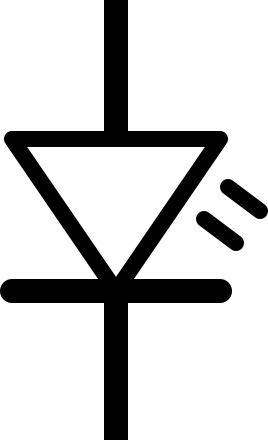
\includegraphics[scale=0.125]{LEDSymbol.png} & LED & An LED is represented by an arrow with a line across it, indicating that current can flow from positive to negative in the direction of the arrow, but it is blocked going the other way.  The LED symbol also has two short lines coming out of it, representing the fact that it emits light. \\
\end{tabular}
\end{center}
\end{figure}

Then, the components are connected together using lines to represent the wires and connections between the components.

Therefore, we can redraw our original circuit using these symbols like you see in Figure~\ref{figCircuitBasicLED}.

\begin{figure}
\caption{Basic LED Circuit Drawn as a Diagram}
\label{figCircuitBasicLED}
\centering
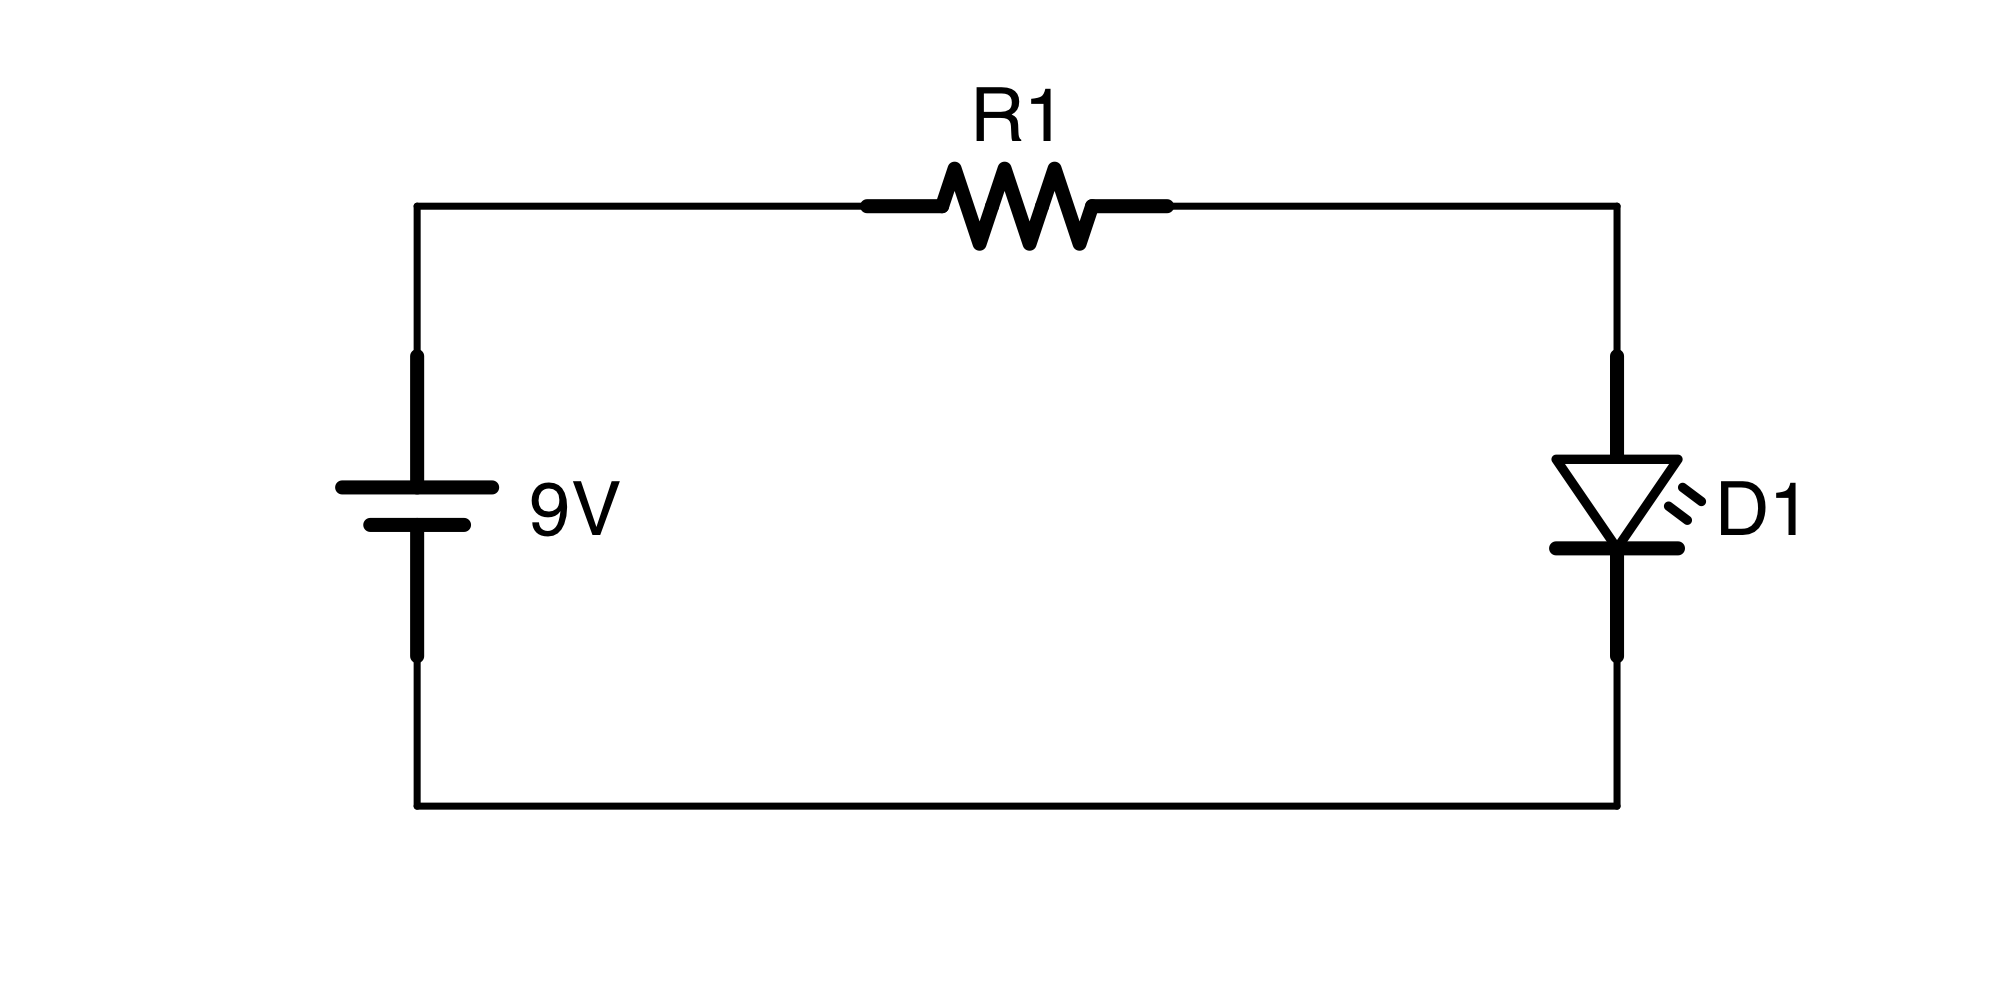
\includegraphics[scale=0.125]{CircuitBasicLED.png}
\end{figure}

Notice that each of our components are laid out on the diagram with wires connecting them.
Remember that it doesn't matter if we have very long wires, very short wires, or if the components are directly placed end-to-end---the resulting circuits will operate identically.
Also notice that each component is labeled (R1 and D1) because, as we make more complicated circuits, it is important to be able to refer back to them.

It does not matter in a diagram which way you have your components turned, how long or short your wires are, or what the general spacing looks like.
When you actually wire it, all of those things will change.
The important part of a circuit diagram is to convey to the reader what the parts are, how they are connected, and what the circuit does in the way that is easiest to read.

For instance, all of the circuits in Figure~\ref{figCircuitLEDAlt} are equivalent to the circuit in Figure~\ref{figCircuitBasicLED}, they are just drawn differently.

\begin{figure}
\caption{Alternative Ways of Drawing the Basic LED Circuit}
\centering
\label{figCircuitLEDAlt}
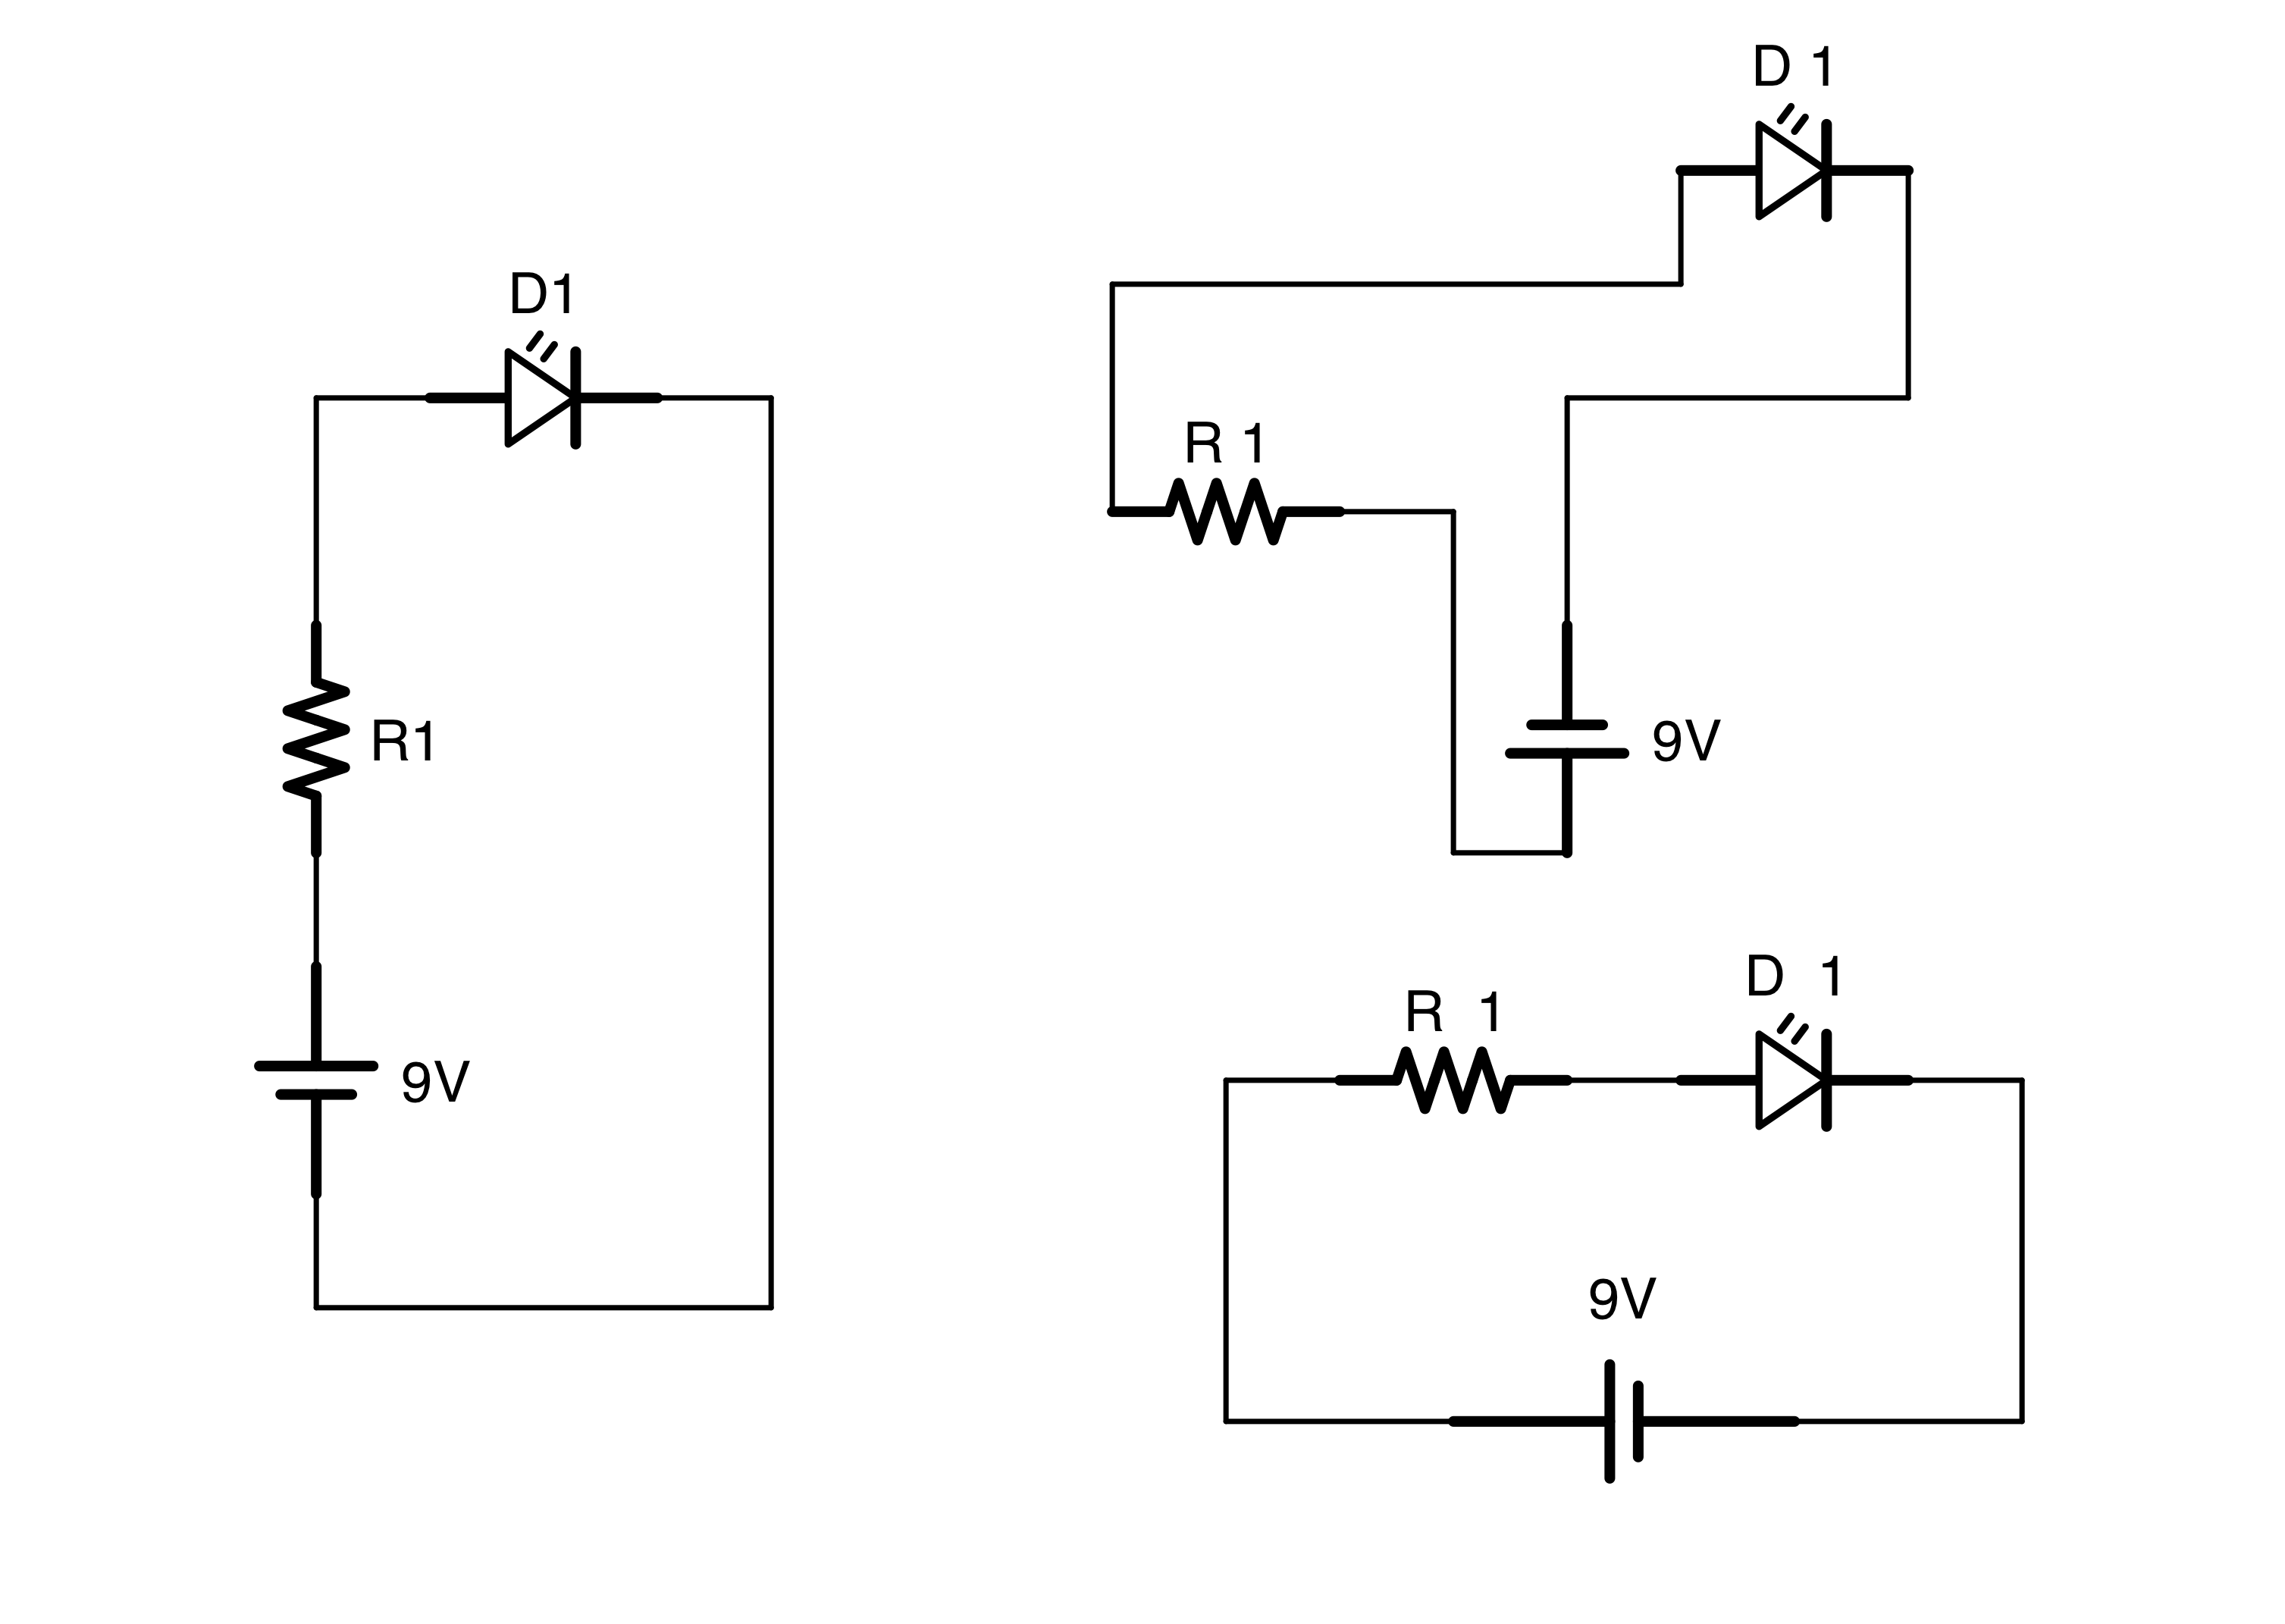
\includegraphics[scale=0.08]{CircuitLEDAlt}
\end{figure}

For consistency, I like to draw all of my batteries to the left of the drawing with the positive side on top.
By keeping the battery positive-side-up, components with higher voltage are usually closer to the top, and components with lower voltages are usually closer to the bottom, with the ground (i.e., zero volts) coming back into the negative terminal.
I also try to make my wire lines as simple as possible in order to make following them easier.

By keeping some amount of consistency, it is easier to look at a drawing and see what it happening.

\section{Drawing the Ground}

Remember that for electricity to move, every circuit must be fully connected from the positive side to the negative side.
That means that in larger circuits there are numerous connections that come from the positive or go back to the ground/negative.
Because of this, a special symbol has been adopted to refer to the ground point in a circuit.
This symbol, the ground symbol, has three lines, each shorter than the next.
Every point on a circuit that has this symbol connected to it is connected to each other (usually they are all connected to the negative side of the battery).

Therefore, the circuit in Figure~\ref{figCircuitBasicLEDGround} is the same circuit as before, just drawn using the ground symbol.
Since every point with the ground symbol are all connected together, using this symbol on both the negative terminal and the negative side of the LED means that they are wired together.

This doesn't help us a lot for this circuit (and, in fact, it makes it a little less easy to read).  
However, in complex circuits, it is much easier to write the ground symbol than trying to have twenty lines drawn back to the negative terminal.

\simplegraphicsfigure{Basic LED Circuit Drawing Using the Ground Symbol}{CircuitBasicLEDGround}{0.08}

Additionally, the same is true with the positive side of the battery.
Many components require a direct connection to a specific voltage to work correctly.
These are usually marked with just a disconnected wire with the end of the wire marking what voltage it requires.
We make less use of that symbol in this book than the ground symbol, but it does come in handy sometimes.

So, using both the voltage source and the ground symbols, we could rewrite the same circuit again in the manner shown in Figure~\ref{figCircuitBasicLEDPosGround}.
This circuit, again, is not \emph{wired} any differently than before.
We are just \emph{drawing} it differently.
For this circuit, it doesn't matter, but in more complex circuits, if we need a specific voltage at a specific location, this symbol tells us to put it there.

\simplegraphicsfigure{Simple LED Circuit Using Positive and Ground Symbols}{CircuitBasicLEDPosGround}{0.08}

\reviewsection

In this chapter, we learned:

\begin{enumerate}
\item Every circuit requires a source of power (usually a battery), wires and components, some amount of resistance, and a complete path back to the negative side of the power source.
\item An open circuit is one that does not connect back to the negative side (and thus does not provide any electricity), and a short circuit is one that connects back to the negative side without any resistance (and thus overwhelms the circuit with current).
\item Batteries supply a fixed voltage between its two terminals.
\item A resistor provides a fixed resistance (measured in ohms) within your circuit.
\item An LED allows current to flow in only one direction, gives off light when current is flowing, but is destroyed when the current goes above 20--30 milliamps.
\item The longer leg of the LED should be on the positive side of the circuit.
\item Wires on a circuit can be almost any length (from zero to a few meters) without changing the functionality of the circuit.
\item A circuit diagram is a way of drawing a circuit so that it is easy to read and understand what the circuit is doing.
\item Each component has its own symbol in a circuit diagram.
\item Every component labeled with the ground symbol is connected together, usually at the negative side of the battery.
\item Voltage sources can be similarly labeled by a wire connected on one side labeled with the voltage that it is supposed to be carrying.
\end{enumerate}

\applysection

\textbf{Special Note} - In the problems below, since we have not yet studied LED operation in-depth, we are ignoring the electrical characteristics of the LED and just focusing on the resistor.  
If you know how to calculate the circuit characteristics using the LED, please ignore it anyway for the purpose of these exercises.

\begin{enumerate}
\item Calculate the amount of current running in the circuit you built in this chapter using Ohm's law.  Since Ohm's law gives the results in amps, convert the value to milliamps.
\item Let's say that the minimum amount of current needed for the LED to be visibly on is 1 milliamp.  What value of resistor would produce this current?
\item Let's say that the maximum amount of current the LED can handle is 30 milliamps.  What value of resistor would produce this current?
\item Draw a circuit diagram of a short circuit.
\item Take the circuit drawing in this chapter, and modify it so that it is an open circuit.
\item Draw a circuit with just a battery and a resistor.  Make up values for both the battery and the resistor and calculate the amount of current flowing through.
\end{enumerate}

\chapter{Constructing and Testing Circuits}
\label{chapConstructingTesting}

%% FIXME - show examples of connected and unconnected wires, and components placed wrongly if I haven't done so already.

In the previous chapter, we learned the theory behind how to analyze circuits.
In this chapter, we are going to put real circuits together and use simple equipment to analyze the same kinds of problems, and compare our calculated answers to the measurements we make on live circuits.

\section{The Solderless Breadboard}

The most important piece of equipment to use for making circuits is the \glossterm{solderless breadboard}.
Before solderless breadboards, if you wanted to put together a circuit, you had to attach them to a physical piece of wood to hold them down, and then \glossterm{solder} the pieces together.
Soldering is a process where two wires are physically joined using heat and a type of metal called solder, which melts at much lower temperatures than other types of metal.
So, what you would have to do is attach the electrical components to the board, wrap the components' legs around each other, and then heat them up with a soldering iron and add solder to join them permanantly.

This was an involved process, and, though it was possible to get your components back, you were generally stuck with your results.
The solderless breadboard is an amazing invention that allows us to quickly and easily create and modify circuits without any trouble at all.
Figure~\ref{figSolderlessBreadboard} shows what a solderless breadboard looks like.

\simplegraphicsfigure{A Solderless Breadboard}{SolderlessBreadboard}{0.5}

The solderless breadboard has a number of spring clips (usually about 400 or 800 of them) called \glossterm{connection points} which will allow you to insert wires or component leads and will hold them in place.
Not only that, the breadboard itself will connect the components for you!

The way that this works is that the breadboard is broken up into little half-rows called \glossterm{terminal strips}.
Each terminal strip has multiple connection points---usually five.
Each connection point on a given terminal strip is connected by wire \emph{inside} the breadboard.
Therefore, to connect two wires or leads together, all you need to do is connect them to the same terminal strip.
Any two wires or leads connected to the same terminal strip are themselves connected.

In most breadboards, the two sides of the breadboard are separated by a gulf known as the \glossterm{bridge}.
The bridge is a visual indication that the two sets of terminal strips are not connected, but it also serves a practical purpose.
If you have an integrated circuit (a small chip), the bridge is the right width so that you can place your integrated circuit right over the bridge, and each leg of the chip will receive its own terminal strip for you to easily connect them to what you need.
We will cover this in more depth in later chapters.

\simplegraphicsfigure{Parts of a Solderless Breadboard}{SolderlessBreadboardParts}{0.5}

In addition to the terminal strips, most breadboards have two strips running down each side, one with a red line and one with a blue line.
These are known as \glossterm{power rails} (some people call them \glossterm{power buses}).  

Power rails are very similar to terminal strips, with a few exceptions.
The main difference is that, in terminal strips, only the five connection points grouped together are connected.
On power rails, many more of the connection points are connected together, even when there are short gaps.
Some boards will split the power rails at the halfway point, but others go all the way down the board.  
This is usually visually indicated by a break in the red and blue lines that indicate the power rails.

Note that the positive and negative are \emph{not} connected to each other (that would create a short circuit), and they are \emph{not} connected to the power rails on the other side of the breadboard (unless you connect them manually).
As we mentioned, on some breadboards, even a single side isn't connected all the way down, but may be broken into sections at the halfway point.

In many projects, many components need direct access to the positive or negative power supply.
Power rails make this easy by providing a connection point with positive and negative power a very short distance away from wherever you need it on the breadboard.
If you plug your power source's positive and negative terminals into the positive and negative rails on the breadboard, then any time you need a connection to the positive or negative terminal, you can just bring a wire to the closest connection point on the appropriate power rail.

\section{Putting a Circuit Onto a Breadboard}

To see how a simple circuit works on a breadboard, let's go back to the circuit we first looked at in Chapter~\ref{chapFirstCircuit}.
Figure~\ref{figCircuitBasicLEDRepeat} has the drawing again for ease of reference.

\begin{figure}
\caption{Basic LED Circuit}
\label{figCircuitBasicLEDRepeat}
\centering
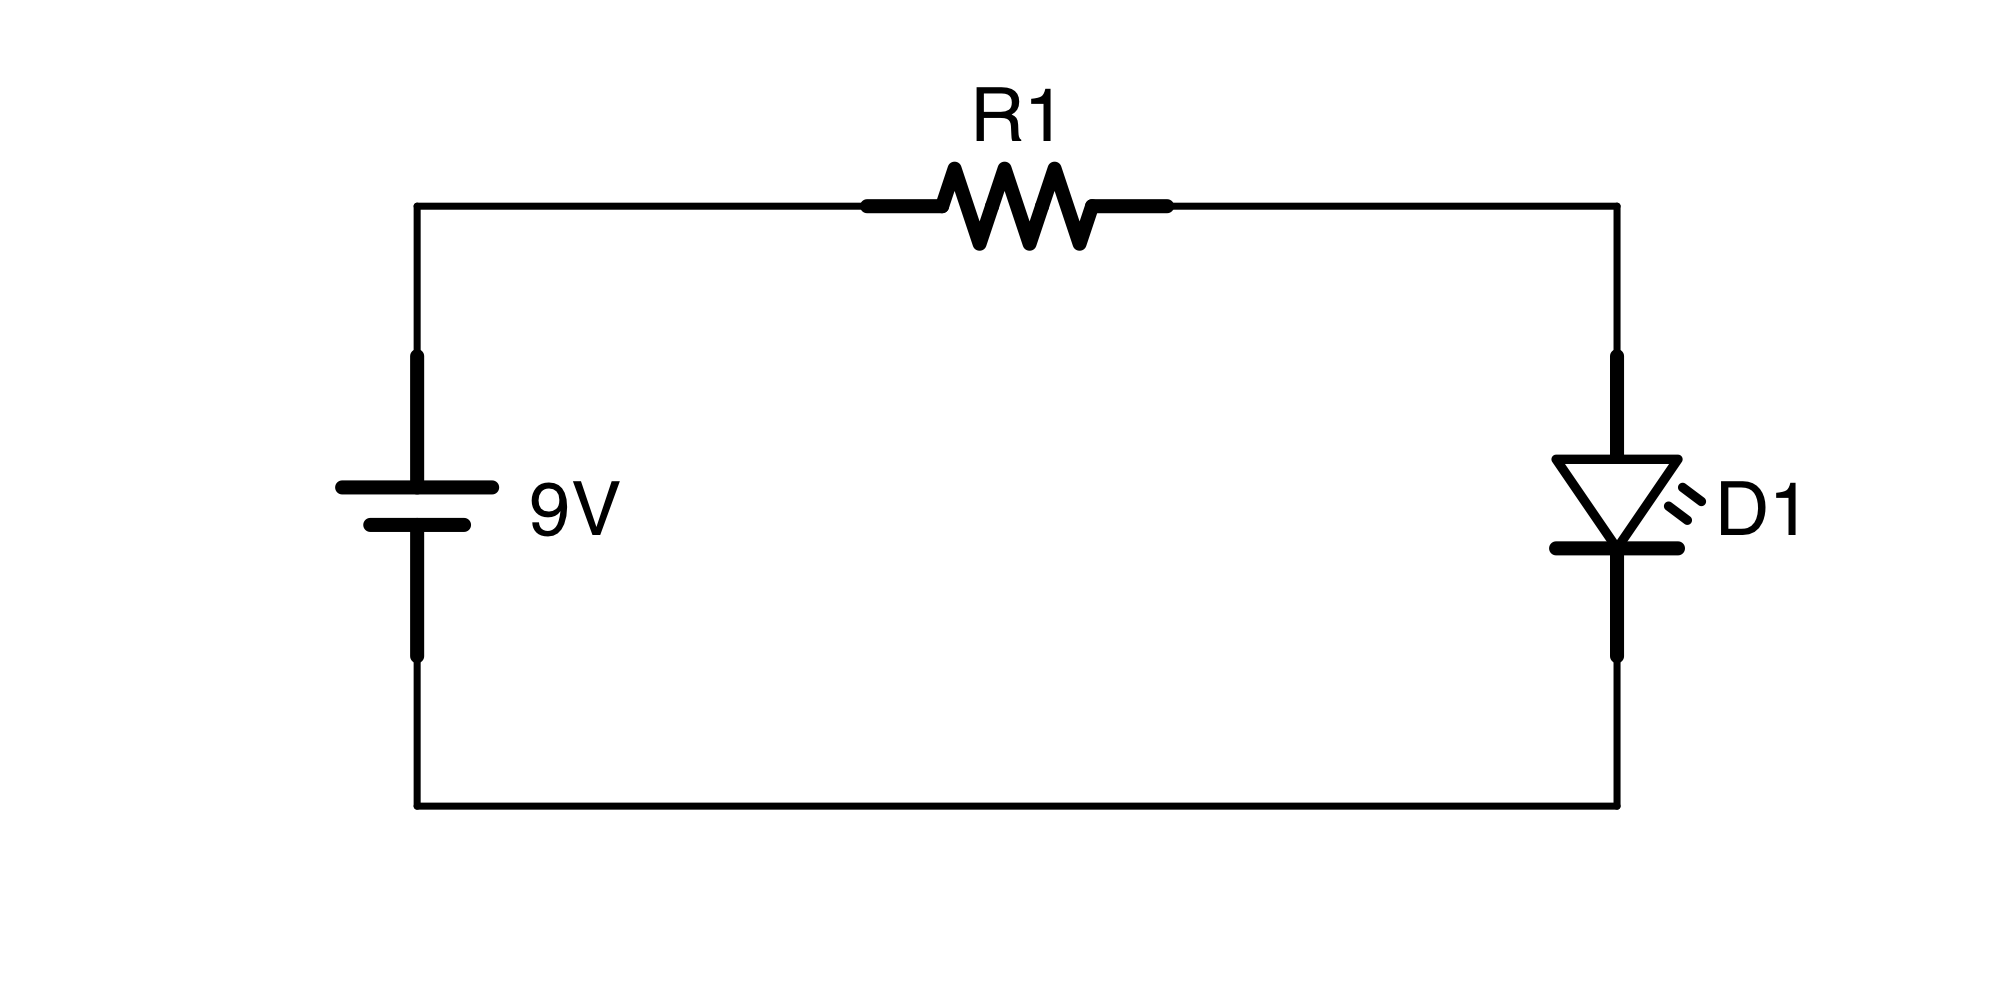
\includegraphics[scale=0.125]{CircuitBasicLED.png}
\end{figure}

So, how do we translate what we see in the drawing to what we need to put in the breadboard?
Well, let's take a look at what is in the circuit---a 9-volt battery, an LED, and a resistor.
Let us not concern ourselves with the battery at the moment.
So, without the battery, we have a resistor connected to an LED.

Let us start out by simply placing our components onto the breadboard.
What you will want is to place them on the breadboard so that each of their legs are on \emph{different} terminal strips.
It doesn't matter \emph{which} terminal strips you use---just make sure the legs all get plugged into different ones.
Figure~\ref{figBreadboardBegin} shows how your breadboard should look so far.
Note that the longer leg of the LED is closer to the resistor.

Figure~\ref{figBreadboardBadEdited} shows the \emph{wrong} way to do it.
In that figure, the both of the legs of the components are on the same row, which is the same thing as placing a wire between the legs, creating a short circuit.
Don't do that!  Make sure each leg goes into its own row.

\simplegraphicsfigure{Putting the Components onto the Breadboard}{BreadboardBegin}{1}

\simplegraphicsfigure{The Wrong Way to Put Components onto the Breadboard}{BreadboardBadEdited}{1}

Now, to connect the resistor to the LED, we need to add a wire.
So, all we need to do is connect a wire to any empty connection point that is on the same terminal strip of the right leg of the resistor, and connect the other side of that wire to the left leg of the LED as shown in Figure~\ref{figBreadboardBeginTwo}.

\simplegraphicsfigure{Adding a Wire to Connect the Components}{BreadboardBeginTwo}{1}

A common mistake that people will make is to connect the wire to the row right before or after the component.
Take some time and be extra certain that the wire is connected to the same row as the leg of your components.

Now, we need to connect our project to the power rails.
So, take a red wire from the left leg of the resistor to the positive power rail (remember, as long as it is in the same terminal strip as the resistor, they will be connected).
Likewise, take a black wire from the right leg of the LED to the negative power rail.
I always use red wires for connecting to the positive power rail, and black wires for connecting to the negative/ground rail, as it makes it more clear when I am looking at my project what wire carries what.
Your project should look like Figure~\ref{figBreadboardBeginThree}.

\simplegraphicsfigure{Adding Wires to the Power Rails}{BreadboardBeginThree}{1}

Now your project is almost done.
All you need to do now is to connect your power rails to a power supply.
Connect a T-connector to a 9-volt battery, and then connect the red (positive) wire to the positive power rail on the breadboard.  You can plug it in anywhere on the rail, but I usually connect the power to the edge of the rail to leave more room for components.
Then, connect the black (negative) wire to the negative power rail on the breadboard.
As soon as you do this, the LED should light up!
Figure~\ref{figBreadboardBeginFour} shows the final circuit.

\simplegraphicsfigure{Final LED Circuit with Power Connected}{BreadboardBeginFour}{1}

Note that many T-connectors for 9-volt batteries have very flimsy wires that are difficult to insert into a breadboard.
Usually, as long as you can get both terminals in far enough to touch the metal within the connection point, it will work.

% FIXME - need more ways of mitigating this problem

If your circuit doesn't work, here is a list of things to check:
\begin{enumerate}
\item Make sure your battery is properly connected to the breadboard---the red should go to positive and the black to negative.
\item Make sure there are \emph{no} wires directly connecting positive to negative on the board.  Any direct pathway from positive to negative without going through a component will cause a short-circuit and can destroy your components and battery.
\item Make sure that your wires are connected to the same terminal strip as the component lead that they are supposed to be connected to.  If they are on a different row, \emph{they are not connected}!
\item Make sure the LED is inserted in the right way.  The longer leg should be connected to the resistor, and the shorter leg should be connected to the negative power supply.
\item Make sure your components are good.  Try replacing your LED with another LED to make sure it works.
\item If all of those things fail, take a picture of your project and post it to the forum mentioned in Chapter~\ref{chapIntro}.  Someone will likely be able to spot your problem and/or lead you in the right direction.  Many other forums are also available on the web for this.
\end{enumerate}

\section{Using Fewer Wires}

In the previous section, we used three wires to connect our components, plus two more wires from the battery.
We can improve our project by reworking it so that most of the wires are not necessary.

Remember that any two leads or wires plugged in next to each on the same terminal strip are connected.
Therefore, we can remove the wire that goes from the LED to the resistor simply by moving the LED and resistor so that the right leg of the resistor is on the same terminal strip.
Figure~\ref{figBreadboardFewerOne} shows what this looks like.

\simplegraphicsfigure{Joining Components by Putting Their Leads on the Same Terminal Strip}{BreadboardFewerOne}{1}

However, that middle wire is not the only redundant wire.  
If you think about it, we could also save a wire by actually using the LED's own leads to go back to the negative rail.
Figure~\ref{figBreadboardFewerTwo} shows how this is setup.
Now, in order to make the LED fit better, it is now on the \emph{other} side of the resistor in the terminal strip.
Remember that this does not matter at all!
No matter where a component is connected on the terminal strip, it is joined with a wire to every other component on the same terminal strip.

\simplegraphicsfigure{Directly Connecting the LED to the Negative Rail}{BreadboardFewerTwo}{1}

Now, there is one last wire that we can get rid of.  
Can you think of which one it is?
If you said the wire going from the positive rail to the resistor---you were right.

What we can do is to directly connect the resistor to the positive rail.
Doing this gives us what is shown in Figure~\ref{figBreadboardFewerThree}.

\simplegraphicsfigure{Connecting the Resistor Directly to the Positive Rail}{BreadboardFewerThree}{1}

Therefore, as you can see, there are any number of ways that you can arrange parts on a breadboard to match a given schematic.  
All of these arrangements we have seen match the schematic given in Figure~\ref{figCircuitBasicLEDRepeat}.
As long as your circuit matches the configuration in the schematic, the specifics of where you put the wires and components is up to you.
Some people like to place the components on their breadboard first, spaced out, and then add wires to connect them as needed.
This works, though it does make for a messier board.
Other people like to use as few wires as possible, and have their layouts as clean as possible (i.e., they don't like a tangled mess).

Some people like to use flexible jumper wires, that goes up and over the board.
Other people like to use rigid jumper wires that lay down close to the board and is the exact length needed.
The flexible wire allows more flexibility in building your circuits (they are easier to move around and reconfigure), while the solid, rigid wire makes the final result a lot cleaner and easier to follow.

You can also trim the legs of your components to make them fit better, if you want.
Some people like to leave their components as intact as possible, while others like to trim the legs of their leads to be the exact right size for their project.
However, if you do trim the leads on your LEDs, be sure to keep the positive leg longer!

However you like to work with electronics is up to you. 
There are lots of options, and they all end up with the same circuit.

\section{Testing Circuits with a Multimeter}

Now that we know how to put circuits together, we need to know how to \emph{test} our circuits.
The main tool used to test simple circuits is the \glossterm{multimeter}.
It is called a multimeter because it measures \emph{multi}ple different things about a circuit.

There are a lot of different multimeters around which have a lot of different functions.
However, almost all of them will measure voltage, current, and resistance.
Each of these values are measured by testing two different points on the circuit.
Most multimeters have a red lead and a black lead.
The red lead should connect to the more positive side of the circuit, and the black lead should connect to the more negative side of the circuit.
However, if you get it reversed, it is usually fine---the multimeter may just report negative values if you are measuring for voltage or current.

\simplegraphicsfigure{A Low-Cost Multimeter}{Multimeter}{0.1}

To illustrate how to use a multimeter, we will start out measuring the voltage in a 9-volt battery.
Remember from Chapter~\ref{chapVoltageResistance} that there is no absolute zero voltage---voltages are merely measured with reference to each other.
Therefore, a multimeter doesn't tell you the exact voltage of something---there is no exact voltage.
Instead, a multimeter allows you to choose two points on your circuit and measure the voltage difference (also known as the \glossterm{voltage drop}) between them.

Now, remember that a 9-volt battery means that the battery should have 9 volts between its positive and negative terminals.
Don't try it yet, but when we measure voltage, we will expect that the multimeter will tell us that the voltage difference is near 9 volts.

When using your multimeter, you must set \emph{what} you are going to test \emph{before} you test it.
Otherwise, you can easily damage your multimeter or your circuit.
Therefore, since we are going to measure voltage, select the DC Voltage setting on your multimeter (\emph{do not} select the DC Current or DC Amperage setting!).
If you are using a high-quality \glossterm{auto-ranging} multimeter, that is all you need to do.
However, when starting out, most people buy the bottom-of-the line multimeter.
That's not a problem, but just know that you will probably accidentally break it at some point.

If you are using a lower-quality multimeter, you will need to not only select \emph{what} you want to measure, but the \emph{estimated range} of values that you want to measure.
On my multimeter, the DC Voltage has five different settings---\icode{1000}, \icode{200}, \icode{20}, \icode{2000m}, and \icode{200m}.
These are the upper boundaries (in volts) that these settings can read (though \icode{2000m} and \icode{200m} indicate millivolts).
Additionally, they indicate the ranges that these settings are best at reading.

So, for a 9-volt battery, using the 1,000-volt setting is probably unwise.
It may give a reading, but it probably won't be accurate.
However, if I try it on too low of a setting (say, 2000m), it either won't read, or it will blow out my multimeter.
So, the safe thing to do is to start with the highest reasonable setting (or just the highest setting if you don't know what's reasonable), test it, and the reduce the setting until it gives you a good reading.

So, for instance, for my 9-volt battery, let's say I didn't know the voltage.
Therefore, I'm going to measure the battery using the 1,000-volt setting.
After setting the multimeter to 1,000 volts, I will put the red lead on the positive terminal of the battery, and the black lead on the negative terminal.
Be sure that you \emph{firmly} press the \emph{tip} of your leads against the positive and negative terminals.  
If it is not firm, or if you use the sides of your terminals, you will not get a good reading.

When I do this, my multimeter reads \icode{9}.  

Now, notice that this reading is significantly less than our 1,000-volt setting.
Therefore, it may not be entirely accurate.  
So, I will reduce the setting to the 200-volt setting and measure again.
This time, my multimeter reads \icode{9.6}.
This is definitely a more accurate reading---it is giving me an extra digit of accuracy!
However, this reading is still significantly below the setting.

Therefore, I will reduce the setting again to the 20-volt setting and re-measure.
This time, the measurement is \icode{9.66}.
Again, it is more accurate.
Now, can I reduce the setting even more?
Well, the next setting is \icode{2000m}, which is basically 2 volts.
Our current reading is 9.66 volts, so it is above the cutoff point for the next setting.
Therefore, I should not try it on a lower setting, both for the sake of accuracy and for the sake of my multimeter's lifespan.

However, I should note that if I did use a lower setting, since the setting is listed as being in millivolts (i.e., \icode{2000m}), then the reading will also be in millivolts.  
That is, if we were to read the value of the battery on that setting, it would say \icode{9660}, because that is how many millivolts the battery has.

Now, you could be wondering, why is a 9-volt battery anything other than exactly 9 volts?
Well, it turns out that in electronics, no value is exact, and no formula works perfectly.
When we talk about a 9-volt battery, we are actually talking about a battery that runs anywhere from 7 volts to 9.7 volts.
In fact, my battery that started out at 9.66 volts will slowly lose voltage as it discharges.
This is one of the reasons why measurement is so important.

Also, this means that in our circuits we will have to find ways to compensate for varying values.
Our circuits should work across a wide range of possible values for our components.
We will discuss strategies for this as we go forward.

The next thing we will measure is resistance.
Pull out a resistor---any resistor.
Appendix~\ref{appendixResistorValues} shows you how to find the resistor values based on the color bands on the resistor.
I don't know about you, but my eyes are not that good at looking at those tiny lines on the resistor and figuring out which color is which.
Many times, it is easier just to test it with the multimeter.

The process is the same as with measuring the voltage.
First, find the resistance settings on your multimeter (perhaps just marked with the symbol for ohms---\si{\ohm}).
Start with the largest value (\icode{2000k}) in my case (\icode{k} means 1,000, so this is a 2,000,000 ohm setting).
On this setting, the multimeter read \icode{000}.
So, I turned it down to the next setting, \icode{200k}.  
This time, it read \icode{00.2}.
So, since the setting is listed in \icode{k} (thousands), this means that the resistor is probably around $0.2\,\si{\kilo\ohm}$, or around $200\,\si{\ohm}$.
However, this is still not an accurate setting.

Next, I turned the dial down to the next setting, which is \icode{20k}.
When I read it this time, it said \icode{0.22}, which would be about $220\,\si{\ohm}$.
Notice how, as the settings on the multimeter get closer to the actual value, I get more and more accuracy.

Next, I turn the dial down to the \icode{1000} setting, since this is still higher than the $220\,\si{\ohm}$ measured so far.
When I read it this time, it says \icode{218}.  
Since the setting does not have a \icode{k} in the name, that means that this reading is $218\,\si{\ohm}$.
On my multimeter, the next setting is \icode{200}, which is less than my last reading, so I will stop and say that my resistor is a $218\,\si{\ohm}$ resistor.

Note that you should \emph{never test for resistance in a live circuit}.
The multimeter uses power to measure resistance, and if there is already power in the circuit, it can damage the multimeter and/or the circuit.

\section{Using a Multimeter with a Breadboard}

We can use our multimeter with our breadboard, too.
Let's say that we wanted to measure the voltage between the positive and negative rails of the breadboard.

There are two ways to do this.
The first, if the size of your multimeter probes and the size of your breadboard connection points allow it, is to simply shove the leads of your multimeter into connection points on the positive and negative rails.
Since these will be connected to the power by a wire, these will be at the same voltage levels as the battery itself.

However, if your breadboard/multimeter combination does not support this, you can do the same thing by simply connecting two jumper wires into the positive and negative rails, and then testing the voltage on the other end of the wires.  

Also, if you are testing components for voltage, you can also use your multimeter on the exposed legs of the component.
This is often easier than either trying to push your leads into the breadboard or running extra wires to your multimeter.

To try out using your multimeter with your breadboard, configure your breadboard similar to Figure~\ref{figBreadboardBeginFour}.  
Use this layout, and \emph{not} one of the ones with fewer wires (you will see why in a minute).
With the battery connected to the breadboard, set your multimeter to the highest voltage setting, and put the red lead in any empty hole in the positive rail.
While that lead is there, put the black lead in any empty hole in the negative rail.

This should give you the same reading that you received for the battery terminals.
Remember that the power rails are connected all the way across---that is why putting your leads in any hole on the line works!
If you work your way down the ranges on your multimeter, you should find that you get the same value that you did when you measured directly on the battery's leads.
Again, if your leads do not fit inside the connection points, you can also use wires to connect out from your breadboard to your multimeter leads.

You can now do the same to any component on your board.
Let's find the voltage difference between one side of the resistor and the other.
To do this, find an empty hole on the same terminal strip as the left-hand side of the resistor, and put the red lead from your multimeter in that hole.
Then, find an empty hole on the same terminal strip as the right-hand side of the resistor, and put the black lead from your multimeter in that hole.
Now you can measure the voltage difference.
Note that to measure voltage differences, the circuit \emph{must} be active.
If the power is gone, the voltage difference will likely drop to zero.
Use the same ranging procedure to find the voltage drop between the left-hand and right-hand side of the resistor.

Even though we have not discussed diodes, this doesn't prevent you from measuring the voltage difference between the legs of the diode in your circuit.
Use the same procedure as before to measure the voltage drop.

\section{Measuring Current with a Multimeter}

Now we will learn to measure current using the same circuit layout from Figure~\ref{figBreadboardBeginFour}.
Like voltage, measuring current requires that the power to your circuit be on.
To measure current, use the DC Amperage (sometimes called DC Current) settings on your multimeter.

Measuring current is a little different than measuring voltage in a circuit.
Instead of just placing your leads in the breadboard as it is, you are going to use your leads to \emph{replace a wire}.
You will remove a wire, and then place your leads in the holes (connection points) where the wire used to be.
Alternatively, if your multimeter does not fit into the connection points, you can again run two wires, one from each hole, from the breadboard to your multimeter leads.

Using either of these approaches, the circuit will then use your multimeter as the wire that was removed, and the multimeter will then measure how much current is running through that wire, and report it to you on the screen.
You will then need to use the same ranging technique as you used before with voltages and resistances to get an accurate report.

Let's say that you wanted to measure the current going through the wire that connects the resistor to the LED.
To do this, we will start by \emph{removing} that wire, and connecting the red lead to where the wire used to be on the left (since it is more positive), and the black lead to where the wire used to be on the right (since it is more negative).
The multimeter should now report back how much current the circuit is using.  
This will vary for a number of reasons, but should be about $17\,\si{\milli\ampere}$.

Now, put the wire back, and remove another wire and measure current there.
No matter which wire you choose, they should all measure the same current.
The reason is that, since all of these components are in series (one right after the other), they must all have the same amount of electricity flowing through them (otherwise, where would the electricity be going?).

\reviewsection

In this chapter, we learned:

\begin{enumerate}
\item Solderless breadboards can be used to quickly create circuits.
\item Solderless breadboards allow circuits to be easily constructed and destructed in such a way that the components are reusable from one project to the next.
\item Both wire and the legs of a component are attached to connection points on the breadboard.
\item Connection points in the same terminal strip are connected by a wire behind the breadboard.
\item To connect two components together, all you have to do is put their legs on the same terminal strip of the breadboard.
\item The power rails on a breadboard extend either all the way down the board, or sometimes split at the halfway point.
\item The bridge of a breadboard divides and separates different groups of terminal strips.  This allows a chip to be placed over the bridge, allowing each of its pins a separate terminal strip.
\item The schematic drawing of a circuit can be assembled onto a breadboard, giving a definite implementation of the drawing.
\item There are multiple different ways to place a given circuit drawing onto a breadboard.
\item Components on a breadboard can be connected by wires, or they can be connected by placing their legs in the same terminal strip.
\item There are many different styles of placing components onto breadboards, which have tradeoffs between how easy it is to reconfigure, and how clean the result is.
\item A multimeter allows you to measure several important values on a circuit, including resistance, voltage, and current.
\item If your multimeter is not auto-ranging, you must test your value several times, starting with the highest range setting for the value you are looking for, and decreasing it through the settings until you find a precise value.
\item Always be sure your multimeter is set to the right setting \emph{before} measuring.
\item Always turn your circuit off before measuring resistance.
\item Your circuit must be on to measure voltage or current.
\item Voltage is measured by connecting your multimeter to empty connection points in the terminal strips that you want to measure.  This can be done either by putting your multimeter leads directly into the relevant connection points or by running wires from those connection points to your multimeter leads.
\item Current is measured by using your multimeter to replace a wire that you want to measure current running through.
\item Many circuit values vary much more than what you might think, so it is good to design circuits in a way that will handle these variances.
\end{enumerate}

\applysection

All measured values should be measured using the ranging technique discussed in this chapter.

\begin{enumerate}
\item Start with the circuit you built in Figure~\ref{figBreadboardBeginFour}.  Measure the voltage drop across the resistor, then measure the voltage drop across the LED.  Now, measure the voltage drop across both of them (put the red multimeter lead on the left side of the resistor and the black multimeter lead on the right side of the LED).  Write down your values.
\item Using the same circuit, change the LED from red to blue.   Measure the values again and write them down.  Measure the current going through the circuit using any wire.  Is it the same or different than before?
\item Add another LED in series with the one you have already.  Measure the voltage drops between each side of each component in the circuit.  Measure the current going through any given wire.  Write down each value.
\item Take the new circuit you built in the previous problem and draw the schematic for the circuit.
\end{enumerate}

\chapter{Analyzing Series and Parallel Circuits}

% FIXME - do I define "voltage drop" anywhere?

In the Chapter~\ref{chapFirstCircuit} we looked at our very first circuit and how to draw it using a circuit diagram.
In this chapter, we are going to look at different ways components can be hooked together and what they mean for your circuit.

\section{Series Circuits}

The circuit built in Chapter~\ref{chapFirstCircuit} is considered a \glossterm{series circuit} because all of the components are connected end-to-end, one after another.
In a series circuit, there is only one pathway for the current to flow, making analyzing the circuit fairly simple.

It does not matter how \emph{many} components are connected together---as long as all of the components are connected one after another, the circuit is considered a series circuit.
Figure~\ref{figSeriesComponents} shows a series circuit with several components included.

\simplegraphicsfigure{A Series Circuit with Several Components}{SeriesComponents}{0.08}

If all of the components are in a series, then even if there are multiple resistors scattered throughout the circuit, you can figure out the total resistance of the circuit just by adding together all of the resistances.
This is known as the \glossterm{equivalent resistance} of the series.

In this example, if R1 is 100\si{\ohm}, R2 is 350\si{\ohm}, and R3 is 225\si{\ohm}, then the total series resistance of the circuit will be $100 + 350 + 225 = 675\,\si{\ohm}$.

That means that the current is easy to figure out as well.
If we ignore the LEDs (since we have not yet learned to calculate using them), then we can use the total series resistance to calculate current the same way we did with the single resistor.

Since the voltage is 9 volts, then we can use Ohm's law to find out the current going through the system.

$$I = V / R = 9 / 675 = 0.013\,\si{\ampere}$$

Note that \si{\ampere} stands for ampere, and we will be using this in our calculations from here on out.
However, in electronics, we usually measure in milliamps (abbreviated as \si{\milli\ampere}), so let us convert:

$$ 0.013 * 1000 = 13\,\si{\milli\ampere}$$

So, our circuit will draw about 13 milliamps of current.
This amount of current is the same amount running through all of the components in the series.

\section{Parallel Circuits}

Circuits are wired into a \glossterm{parallel circuit} if one or more of their components are arranged into multiple branches.

Figure~\ref{figSimpleParallel} shows a simple circuit with two resistors in parallel.
In this figure, the circuit has \emph{two} branches.
R1 is in the first branch, and R2 is in the second branch.
The place where the branch occurs is called a \glossterm{junction}, and is usually marked with a dot to show that all the wires there are connected.

\simplegraphicsfigure{Two Resistors Wired in Parallel}{SimpleParallel}{0.08}

In a parallel circuit, electricity will flow through both branches simultaneously.
Some of the current will go through R1 and some of it will go through R2.
This makes determining the total amount of current more difficult, as we have to take into account more than one branch.

However, there are two additional laws we can use to help us out, known as \glossterm{Kirchoff's circuit laws}.
The guy's name is hard to spell, but his rules are actually fairly easy to understand.

\subsection{Kirchoff's Current Law}

The first law is known as \glossterm{Kirchoff's current law}.
Kirchoff's current law states that, at any junction, the total amount of current going \emph{into} a junction is exactly the same as the total amount of current going \emph{out} of a junction.
This should make sense to us.
Think about traffic at a four-way intersection.
The same number of cars that enter that intersection must be the same number of cars that leave the intersection.
We can't create cars out of thin air, therefore each car leaving must have come in.
Cars don't magically disappear, therefore each car entering must leave at some point.
Therefore, Kirchoff's circuit law says that if you add up all of the traffic going in it will equal the amount going out.

\begin{advsidebar}{Another Way of Looking at It}
Another way to say this is that the total amount of all of the currents at a junction is zero.
That is, if we consider currents coming in to the junction to be positive and currents going out of the junction to be negative, then their total will be zero since the size of the currents coming in must equal the size of the currents going out.
\end{advsidebar}

So, let's look at a junction.
Figure~\ref{figSimpleJunction1} shows a junction where one wire is bringing current in, and it branches with two wires bringing current out.  
The first wire going out has $0.75\,\si{\ampere}$ of current, and the second wire going out has $0.34\,\si{\ampere}$ of current.
How much current is going into the junction from the left?

\simplegraphicsfigure{A Simple Junction}{SimpleJunction1}{0.08}

Since the total coming in must equal the total coming out, then that means the total coming in must be 

$$0.75\,\si{\ampere} + 0.34\,\si{\ampere} = 1.09\,\si{\ampere}$$

Therefore, the total amount of current coming into the circuit is $1.09\,\si{\ampere}$.

Now, lets say we had a junction of four wires.  
In the first wire, we have $0.23\,\si{\ampere}$ of current coming in.
On the second wire, we have $0.15\,\si{\ampere}$ of current going out.
On the third wire, we have $0.20\,\si{ampere}$ of current going out.
What must be happening on the fourth wire?
Is current coming in or going out on that wire?

To figure that out, we have to look at the totals so far.
Coming in, we have the one wire at $0.23\,\si{\ampere}$.
Going out, we have the two wires for a total of $0.15\,\si{\ampere} + 0.20\,\si{\ampere} = 0.35\,\si{\ampere}$.
Since we only have $0.23\,\myamp$ coming in, but there is $0.35\,\myamp$ going out, that means that the fourth wire must be bringing current in.
Therefore, the amount that this fourth wire must be bringing in is $0.35\,\myamp - 0.23\,\myamp = 0.12\,\myamp$.

\subsection{Kirchoff's Voltage Law}

Kirchoff's current law makes a lot of sense, because the amount of ``stuff'' coming in is the same as the amount of ``stuff'' going out.
This is similar to our everyday experience.
Kirchoff's voltage law, however, is a bit more tricky.
\glossterm{Kirchoff's voltage law} states that, given any two points on a circuit at a particular time, that no matter what path is travelled to get between those two points, the difference in voltage between the two points (known as the \glossterm{voltage drop}) is the same \emph{no matter what pathway you take to get there}.

Figures~\ref{figKirchoffVoltageLawExample0}~and~\ref{figKirchoffVoltageLawExampleComposite} illustrates this point.
If we wanted to measure the voltage drop between the two points indicated (A and B), then that voltage drop, at least at a particular point in time, will be the same no matter what pathway electricity travels.
The direct route between the two points has the same voltage drop as the more winding pathways, no matter what the values of the resistors are.

\simplegraphicsfigure{A Circuit With Many Parallel Paths}{KirchoffVoltageLawExample0}{0.08}
\simplegraphicsfigure{All Paths Between Two Points Have the Same Voltage Drop}{KirchoffVoltageLawExampleComposite}{0.05}

So how does that square with Ohm's law?

The way it works is that Ohm's law will cause all of the \emph{currents} through each part of the circuit to adjust in order to make sure that the \emph{voltage} stays the same.

As you can see, the voltage drop between A and B \emph{must} be 9 volts because the battery is a 9-volt battery, and there are no components (only wires) between the battery terminals and A and B.
Since batteries always have a constant voltage between their terminals, that means that A and B will have the same voltage---9 volts.

Therefore, that means that the voltage drop across R1 is 9 volts, because it is one of the pathways between A and B, and all pathways get the same voltage.
Let's put in some real values for these resistors and see if we can figure out how much voltage and current is happening in each part of the circuit.
Let's set R1 = $1,000\,\si{\ohm}$, R2 = $500\,\si{\ohm}$, R3 = $300\,\si{\ohm}$, R4 = $400\,\si{\ohm}$, and R5 = $800\,\si{\ohm}$.
Now, let's find out what our circuit looks like.

As we have noted, \emph{every} path must have the same voltage drop---9 volts.
So let's start with the easiest one, the current going across R1.
Since we have a 9-volt drop and $1,000\,\si{\ohm}$, we can just use Ohm's law for current: 

$$I = V / R = 9\,\si{\volt} / 1,000\,\si{\ohm} = 0.009\,\myamp$$

So, we have $0.009\,\myamp$ running across R1.

Now, what about R2?
R2 is connected to point A simply by a wire.
As we mentioned in Section~\ref{secWireRule}, wires can be considered to be zero-length.
Therefore, R2 is just as much directly connected to point A as R1 is.
Therefore, the voltage drop across R2 is also going to be 9-volts.
Again, using Ohm's law, we can see that 

$$I = V / R = 9\,\si{\volt} / 500\,\si{\ohm} = 0.018\,\myamp$$

So, the current going across R2 is $0.018\,\myamp$.

What about the current going across R3, R4, and R5?
Well, if you notice, those resistors are all in series, so we can add them all up and just use the total resistance.

So, the total resistance for this section of the circuit will be:

$$R3 + R4 + R5 = 300\,\si{\ohm} + 400\,\si{\ohm} + 800\,\si{\ohm} = 1,500\,\si{\ohm}$$

So, using Ohm's law, the current running through this part of the circuit will be:

$$I = V / R = 9\,\si{\volt} / 1,500\,\si{\ohm} = 0.006\,\myamp$$

Now, remember that the total current flowing into any junction has to be equal to the current flowing out of it.
So, let's look at the junction between R2 and R3.  
We calculated that the current flowing to R2 is $0.018\,\myamp$ and the current flowing to the series starting with R3 is $0.006\,\myamp$.
Therefore, there has to be $0.018 + 0.006 = 0.024\,\myamp$ flowing into that junction.

Now, how much current is flowing out of junction A?
Well, earlier, we noted that the amount of current flowing across R1 was $0.009\,\myamp$, and we just calculated that there is $0.024\,\myamp$ flowing out of A into the junction between R2 and R3. 
That means that there must be $0.033\,\myamp$ total flowing into junction A.

While there were a lot of steps to determine this, each individual step was fairly straightforward.
We simply combined Ohm's law, Kirchoff's voltage law, and Kirchoff's current law to figure out each step.

Now, one important thing to notice is that there is \emph{less} current running through the pieces of the circuit with more resistance than there is with the pieces of the circuit with less resistance.
The electric current is more likely to go down the path of least resistance.
This is a very important point and should not be overlooked, as it will come in handy in later chapters.

\section{Equivalent Parallel Resistance}

The sort of calculation that we have done in the previous section gets trickier if there is a series resistance before or after the parallel resistance.
Figure~\ref{figKirchoffVoltageLawSeriesAndParallel} gives an example of this.
The setup is just like the previous circuit, except there is a single resistor (R6) in series with the battery \emph{before} the parallel branches.
This will prevent our simple calculations from working because the current flowing in each of the branches of the circuit will all add together to tell us the amount of current flowing through R6.
However, the voltage drop across R6 will depend on the current flowing through it.
If this voltage changes, then it will change our starting voltage for our calculations to figure out the parallel branches.

\simplegraphicsfigure{Kirchoff's Voltage Law with Series and Parallel Components}{KirchoffVoltageLawSeriesAndParallel}{0.08}

Thus, we have ourselves in a loop---in order to find out the current flowing through the parallel branches, we have to know their starting voltage.
In order to find out their starting voltage, we have to know how much the voltage dropped across R6.
In order to know how much the voltage dropped across R6, we have to know how much current was flowing through it!

This may seem like an impossible problem, but basic algebra allows us to work it out, though the details are kind of ugly.
Instead, we have an equation which gives us \glossterm{equivalent resistance}.
That is, we can take a series of parallel resistors, and we can calculate the total resistance of those resistors.

If you have resistors in parallel to each other (let's call them $R_1$, $R_2$, and $R_3$), and you want to know the resistance of their \emph{combined} action (which we will call this total $R_T$), then you would use the following equation:

\begin{equation}
\label{eqparallelresistancethree}
R_T = \frac{1}{\frac{1}{R_1} + \frac{1}{R_2} + \frac{1}{R_3}}
\end{equation}

This equation works for any number of resistances that we have in parallel.
We can just keep on adding them to the end of the list:

\begin{equation}
\label{eqparallelresistancen}
R_T = \frac{1}{\frac{1}{R_1} + \frac{1}{R_2} + \ldots + \frac{1}{R_N}}
\end{equation}

So, let's look at our circuit, and see how we can find out the currents flowing through each resistor.
For this example, we will again say that $R1 = 1,000\,\si{\ohm}$, $R2 = 500\,\si{\ohm}$, $R3 = 300\,\si{\ohm}$, $R4 = 400\,\si{\ohm}$, and $R5 = 800\,\si{\ohm}$.  Additionally, $R6 = 250\,\si{\ohm}$.

In order to compute this, we first have to figure out \emph{what} is in series and what is in parallel.
Notice the loop made by R3, R4, and R5.  
Those are all connected end-to-end, so they are in series.
Because they are in series, we can get their equivalent resistance just by adding them together---$300 + 400 + 800 = 1,500\,\si{\ohm}$.
Therefore, we can actually \emph{replace} these resistors with a single, $1,500\,\si{\ohm}$ resistor.
We will call this ``combined'' resistor R7.
Now, if you look at the new picture, with R7 standing in for the loop, you will see that R1, R2, and R7 are in parallel with each other.

Therefore, we can find out their combined resistance by using Equation~\ref{eqparallelresistancen}:

\begin{align*}
R_T &= \frac{1}{\frac{1}{R1} + \frac{1}{R2} + \frac{1}{R7}} \\
R_T &= \frac{1}{\frac{1}{1,000} + \frac{1}{500} + \frac{1}{1,500}} \\
R_T &= \frac{1}{0.001 + 0.002 + 0.00067} \\
R_T &= \frac{1}{0.00367} \\
R_T &= 272.5\,\si{\ohm}
\end{align*}

Therefore, the equivalent resistance of all of the parallel resistances is about $272.5\,\si{\ohm}$, which means that we can replace \emph{all} of these resistors (R1, R2, R3, R4, and R5) with a single resistor that is $272.5\,\si{\ohm}$.
Also notice that this resistance is actually \emph{less} than each of the individual resistances.

Now, to get the total resistance of the circuit, we notice that this parallel resistance ($272.5\,\si{\ohm}$) is in series with R6, which is $250\,\si{\ohm}$.  
Since they are in series with each other, we can simply add them together.
The total resistance of this circuit is $250 + 272.5 = 522.5\,\si{\ohm}$.
We can now use Ohm's law to find the total amount of current running through this circuit:

\begin{align*}
I &= \frac{V}{R} \\
I &= \frac{9}{522.5} \\
I &= 0.0172\myamp
\end{align*}

Thus, the whole circuit has 0.0172 amperes of current running through it.
Using this, we can now go back through and identify how much current and voltage is flowing through each individual piece.

Because the entirety of the 0.0172 amperes is going through the first resistor, that means that the voltage drop of this resistor will be, using Ohm's law:

\begin{align*}
V &= I\cdot R \\
V &= 0.0172 \cdot 250 \\
V &= 4.3\,\si{\volt}
\end{align*}

That means that this resistor will chew up $4.3\,\si{\volt}$.  
This leaves us with $9 - 4.3 = 4.7\,\si{\volt}$ left after the series resistor.

We now know the starting and ending voltages of each branch of the parallel resistors---$4.7\,\si{\volt}$ at the beginning (what we just calculated the voltage to be after the series resistor), and $0\,\si{\volt}$ at the end (because it connects to the negative terminal of the battery, which we have designated as the zero volt reference).

Therefore, we can use Ohm's law to find the amount of current flowing through each of them.
For R1:

\begin{align*}
I &= \frac{V}{R} \\
I &= \frac{4.7}{1,000} \\
I &= 0.0047\,\si{\ampere}
\end{align*}

For R2:

\begin{align*}
I &= \frac{V}{R} \\
I &= \frac{4.7}{500} \\
I &= 0.0094\,\si{\ampere}
\end{align*}

And finally, for the series that is in a loop at the right (R3, R4, and R5):

\begin{align*}
I &= \frac{V}{R} \\
I &= \frac{4.7}{1500} \\
I &= 0.0031\,\si{\ampere}
\end{align*}

Since the loop is all in series, that means all of the resistors in that series will have $0.0031\,\si{\ampere}$ going through them.

If we add all of these currents, we will see that $0.0031 + 0.0094 + 0.0047 = 0.0172\,\si{\ampere}$, which is the amount of current we originally figured out.

What we have learned is that we can replace the entire circuit with a single value for its resistance to figure out how the circuit will behave as a whole.
For a simple circuit like this, having all of these parallel branches doesn't do much, so it may seem pointless.
However, in a real circuit, each of these branches may be, instead of a resistor, a component that has some amount of resistance.
If you know the resistance, you can calculate how much current is flowing through it the same way.

However, we start with only resistors in order to make the problems simpler.

% FIXME - put this somewhere after we talk about LEDs/diodes more in-depth.  A corollary to that law is that if the calculated voltage drop between two components down a particular pathway must be more than another voltage drop by a different pathway, the pathway with the larger voltage drop can be considered to be disconnected.

\section{Wires in a Circuit}

In complicated circuits, sometimes we run out of room and must draw wires on top of each other even though the wires aren't connected.
In this book, we try to make clear which wires are connected by placing a dot on the junction point.
To show two wires that don't connect to each other, but which had to cross because the diagram was too complicated to prevent it, we will show one of the wires as being broken across the intersection point.
Figure~\ref{figJoinedVsUnjoinedEdited} demonstrates the difference.
The wires on the left are joined together as indicated by the dot.
The wires on the right are not joined in any way, they just had to be drawn across each other because of space reasons in the diagram.

\simplegraphicsfigure{Joined Wires (left) vs. Unjoined Wires (right)}{JoinedVsUnjoinedEdited}{0.08}

Also, the lengths of wires that we draw are irrelevant.  
Usually, in simple circuits, we should consider that wires are all zero-length.
If, after a resistor, the voltage in the circuit has dropped to $5\myvolt$, then we can consider that the \emph{whole wire} until the next circuit is at $5\myvolt$.  
If a wire branches into multiple branches, even though each branch will have a different amount of \emph{current} running on the branch, each branch of the wire will all have the \emph{exact same voltage} until they reach another component.

Therefore, in the circuit in Figure~\ref{figEquivalentPoints}, you can see several points labelled A, B, C, D, E, F, and G.
In this circuit, A, B, and C all have equivalent voltages (though not equivalent currents) since there are only wires (and not components) between them.
Likewise, D, E, F, and G all have equivalent voltages since there are only wires between them.  
Also, since D, E, F, and G are all connected to the battery negative (i.e., ground) with no components between them, that means that they are all at zero volts.
Likewise, since A, B, and C are all directly connected to the battery positive with no intervening components, they are all at 9 volts.

\simplegraphicsfigure{Several Points on a Circuit}{EquivalentPoints}{0.08}

\reviewsection

In this chapter, we learned:
\begin{enumerate}
\item In a series circuit, electricity flows in a single line through all of the components.
\item In a parallel circuit, electricity branches and flows in multiple branches.
\item Most real circuits are combinations of series and parallel circuits.
\item When you have resistors together in series, the total resistance of all of the resistors combined is simply the sum of their individual resistances.
\item In a parallel circuit, Kirchoff's Current Law says that the total amount of current entering a branch/junction is the same as the total amount of current leaving the branch.
\item In a parallel circuit, Kirchoff's Voltage Law says that, between any two points on a circuit at a given point in time, the voltage difference between those two points will be identical no matter what pathway the electricity follows to get there.
\item When resistances are in parallel, the total resistance for the parallel circuit is given by the equation $R_T = \frac{1}{\frac{1}{R_1} + \frac{1}{R_2} + \ldots + \frac{1}{R_N}}$.
\item By using these laws in combination, we can predict how current will flow in each part of our circuit.
\end{enumerate}

\applysection

\begin{enumerate}
\item There is a junction in a circuit that has one wire with current flowing in and two wires with current flowing out.  There is $1.25\myamp$ of current coming in, and the first wire going out has $0.15\myamp$ of current going out.  How much current is leaving through the second wire?
\item There is a junction in a circuit that has two wires with current flowing in and two wires with current flowing out.  The first wire with current flowing in has $0.35\myamp$ of current, the first wire with current flowing out has $0.25\myamp$ of current, and the second wire with current flowing out has $0.42\myamp$ of current.  How much current is flowing in on the second incoming wire?
\item At a junction of four wires, wire 1 has $0.1\myamp$ of current flowing in, wire 2 has $0.2\myamp$ of current flowing in, and wire 3 has $0.4\myamp$ of current flowing out.  Is the current in wire 4 going in or out?  How much current is flowing on it?
\item If I have three $100\myohm$ resistors in series, what is the total resistance of the series?
\item If I have a $10\myohm$ resistor, a $30\myohm$ resistor, and a $65\myohm$ resistor in series, what is the total resistance of the series?
\item If I have a $5\myohm$ resistor and a $7\myohm$ resistor in series, what is the total resistance of the series?
\item If I have two resistors in parallel, a $30\myohm$ resistor and a $40\myohm$ resistor, what is the total resistance of this circuit?
\item If I have three resistors in parallel---$25\myohm$, $40\myohm$, and $75\myohm$, what is the total resistance of this circuit?
\item If I have four resistors in parallel---$1,000\myohm$, $800\myohm$, $2,000\myohm$, and $5,000\myohm$, what is the total resistance of this circuit?
\item If I have three resistors in parallel---$100\myohm$, $5,000\myohm$, and $10,000\myohm$---what is the total resistance of this circuit?  Which of the resistors is the total resistance most similar to?
\item Take a look at the following circuit diagram.  If the voltage drop between B and C is 2 volts, and the voltage drop between C and D is 3 volts, what is the voltage drop between A and E?  What is the voltage at E?  What is the voltage at A? \\ 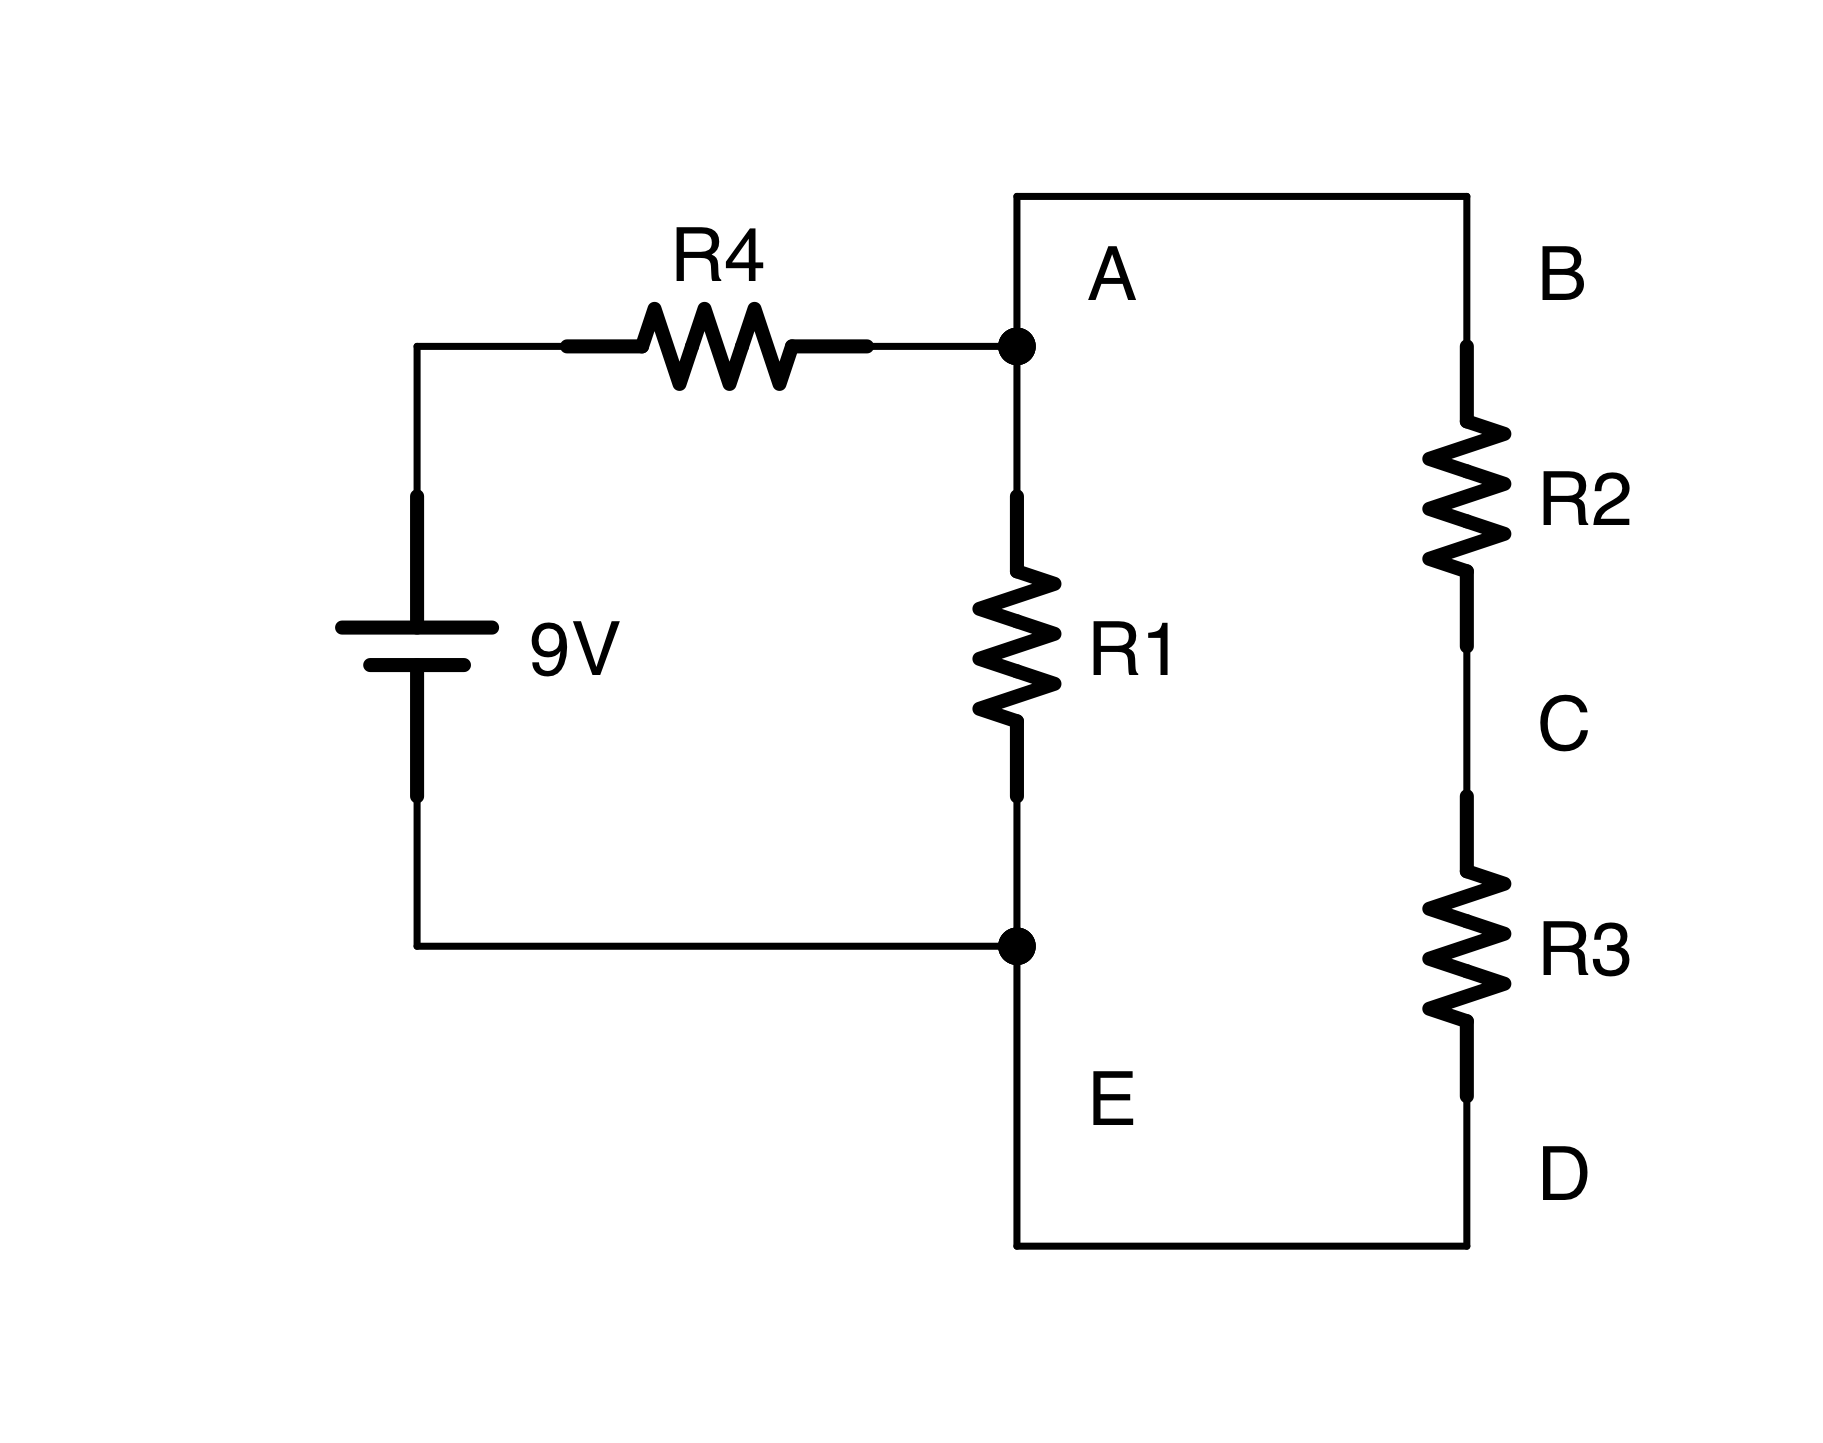
\includegraphics[scale=0.08]{VoltageDropProblem.png}
\item Optional - what resistor values would you need to have the circuit above run with $2\myamp$ total current?
\item The circuit below is a combination of series and parallel resistances.  Each resistor is labelled with its resistance value, given in ohms.  Find out how much current is flowing through each resistor, and how much each resistor drops the voltage.  \\ 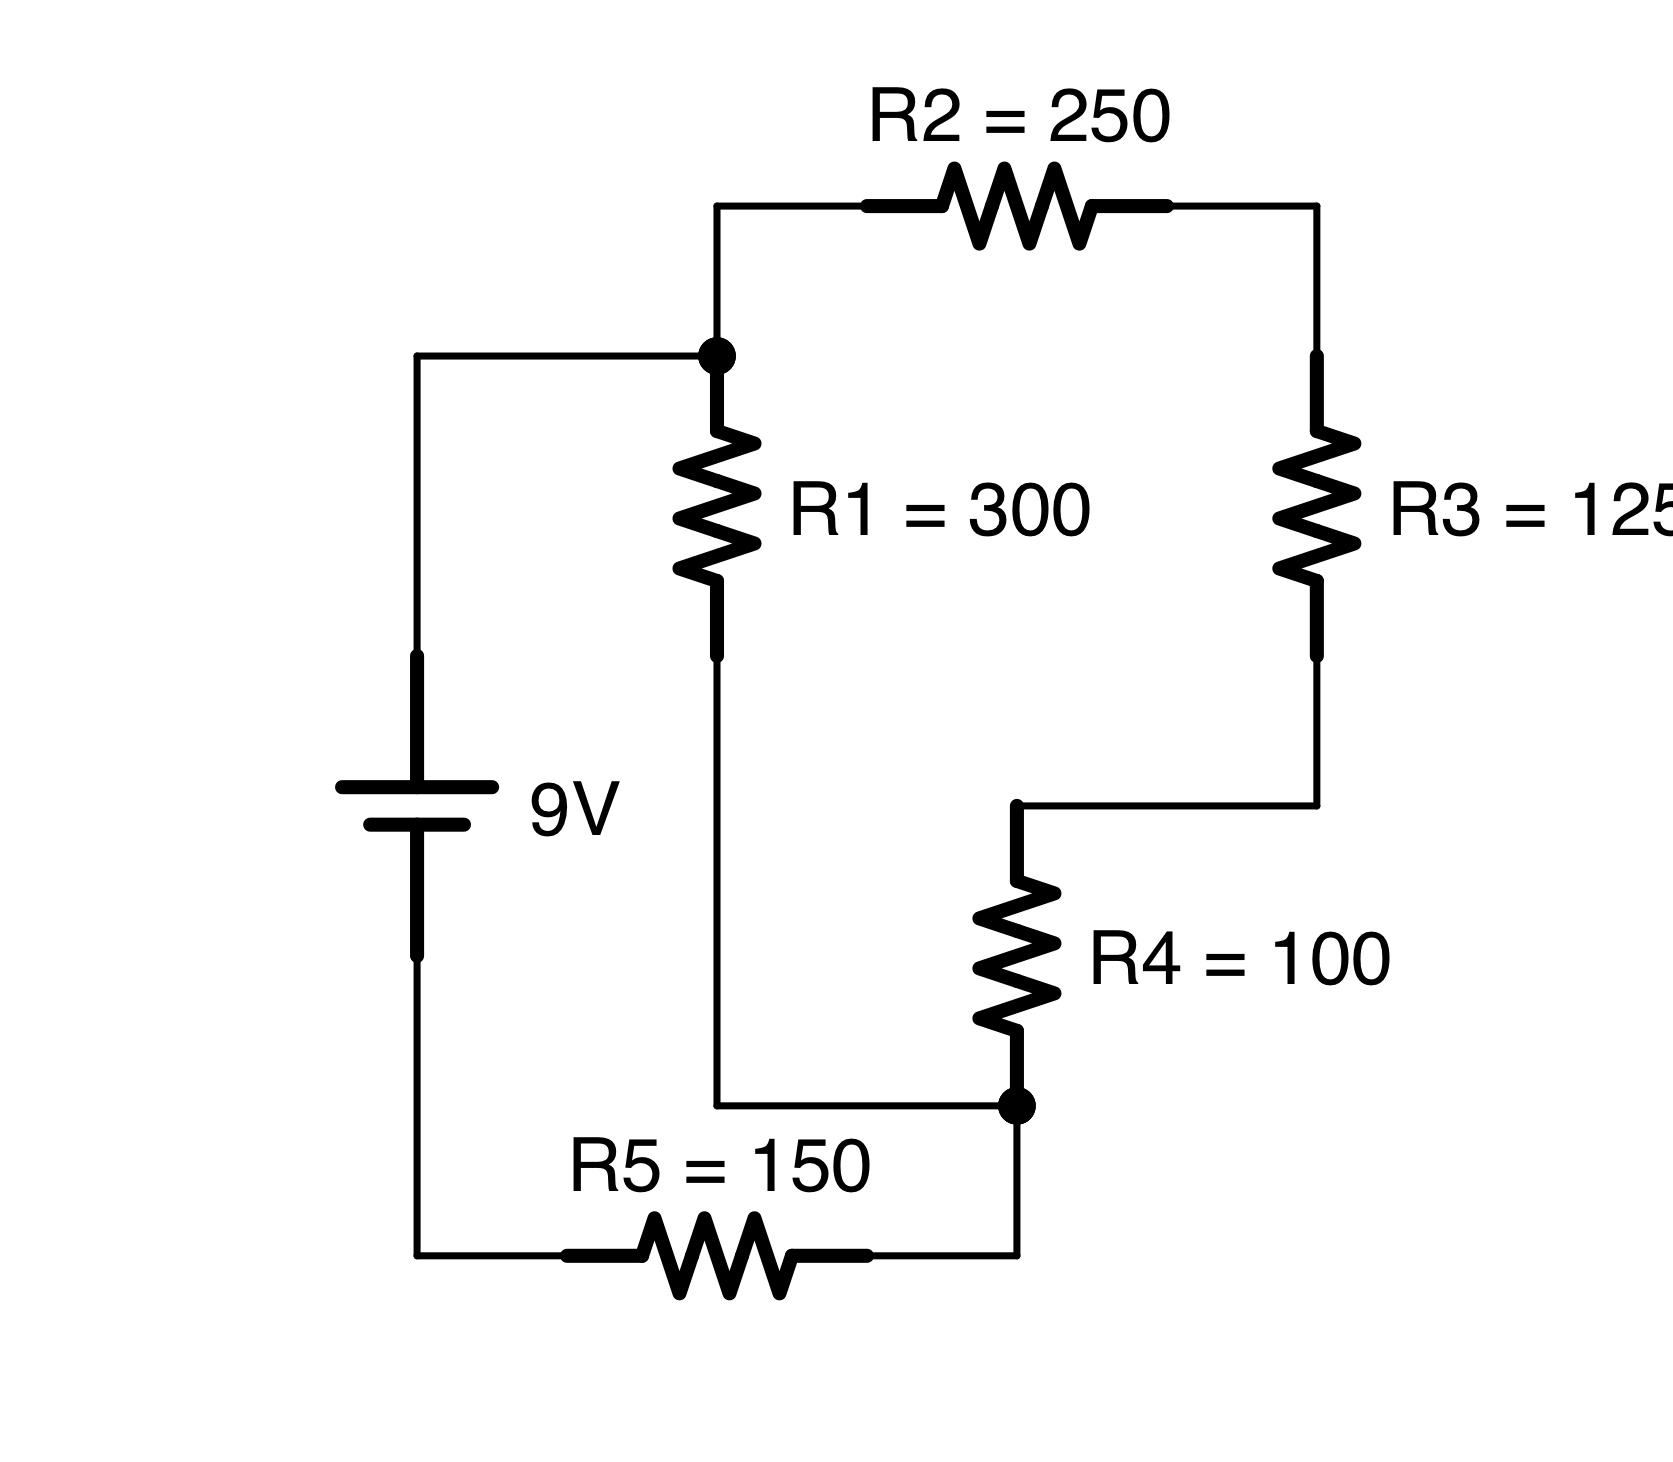
\includegraphics[scale=0.08]{ProblemCalculateCurrentAndVoltage}
\end{enumerate}

\chapter{Diodes and How to Use Them}
label{chapDiodes}

This chapter introduces the \glossterm{diode}.  
We have used light-emitting diodes (LEDs) in previous chapters, but have not really discussed their function except for emitting light.
In this chapter, we are going to look at regular diodes, light-emitting diodes, and Zener diodes, to get a feel for what these devices are and how they might be used in circuits for more than just light.

% FIXME - schematic of a diode

\section{Basic Diode Behavior}

Unlike resistors, diodes have both a positive and negative side.
For any component with both positive and negative legs, the positive leg of the component is termed the \glossterm{anode} and the negative leg is termed the \glossterm{cathode}.
On LEDs, the anode is longer than the cathode.
However, for other types of diodes, the cathode is marked with a line.
You can remember this because in the schematic of a diode, the cathode has the blocking line.

The diode performs two fundamental ``actions'' with electric current.  
The first action of a diode is to drop voltage by an essentially fixed amount \emph{without} affecting or limiting current.
This amount of voltage is called the \glossterm{forward voltage drop} and it is usually around $0.6\myvolt$ for more non-LED diodes. 
Forward voltage is often abbreviated as $\myvolt_F$.
For most LEDs, the forward voltage drop depends on the color of the LED, with a red LED dropping about $1.8\myvolt$ and a blue LED dropping about $3.3\myvolt$.
The forward voltage drop can vary among the other colors as well.

To remind you, when we say ``voltage drop,'' we are referrig to the difference in voltage between the positive and negative leg of the diode.
Therefore, no matter what the voltage is coming into the diode, the voltage coming out of the diode will be that voltage minus the voltage drop.

The second action of a diode is to limit the direction of current to a single direction.
With some exception, the diode only allows current to flow one way in the circuit.
The ``normal flow'' of a current through the diode is to flow from the anode to the cathode.
Looking at the schematic symbol, current flows in the direction that the arrow is pointing, and current is blocked from flowing the other way (you can think of the line as a ``block'' preventing reverse flow).

However, diodes are limited in the amount of reverse flow they can block.
At a certain point, diodes reach their \glossterm{breakdown voltage}.
The breakdown voltage is the voltage at which they will stop blocking voltage.
In regular diodes, this is a failure mode and the precise value shouldn't be relied upon (we will see an exception to this with Zener diodes). %% FIXME - refer to specific section on Zener diodes
Usually, though, this value is high enough not to worry about (i.e., around 100 volts).

\section{Circuit Calculations with Diodes in Series}

Now let's talk about how to properly calculate the behavior of circuits with diodes.
Remember, the key to a diode is that if current is flowing through the diode, the voltage drop across the diode will be essentially constant.
For a normal non-LED diode, this voltage drop is almost always $0.6\myvolt$.
This is so common it is usually assumed, and never listed in the circuit itself.

Therefore, take a look at the circuit in Figure~\ref{figDiodeWithResistor}.
Since the voltage source is 9 volts, that means that the total voltage drop between the positive and negative is 9 volts.
The diode will eat $0.6\myvolt$ of the voltage, but will not limit the current in any way.
The resistor, then, since it is the only component left, will use up the rest of the voltage---$8.4\myvolt$.
Therefore, we can calculate the current in the circuit using Ohm's law:

$$I = V / R = 8.4 / 1000 = 0.0084\myamp = 8.4\mymamp$$

\simplegraphicsfigure{A Diode and Single Resistor Circuit}{DiodeWithResistor}{0.08}

Therefore, our circuit will use $8.4\mymamp$ of current.
So, as you can see, when doing calculations, the diodes simply provide a drop in voltage, they do not limit current.

This is true no matter how many diodes or resistors I have in my circuit.
Figure~\ref{figMultipleDiodesResistors} shows a circuit like that.
To figure out the behavior of this circuit, remember that \emph{every} diode has a $0.6\myvolt$ voltage drop.  Since the circuit has three diodes, that means that the diodes will drop a total of $0.6 * 3 = 1.8\myvolt$.

Therefore, we will have $1.8\myvolt$ taken up by diodes, which drop voltage without limiting current.  
Since we have a $9\myvolt$ source, there will be $9 - 1.8 = 7.2\myvolt$ that is not eaten by diodes.
This voltage will go to our two resistors.  
These resistors, even though they are separated by diodes, are essentially in series with each other.
Therefore, we can treat them as a single resistor in series.
So, the total resistance on the circuit will be $1k + 2k = 3k\myohm$.

We can then find the total current running through the circuit using Ohm's Law:

$$ I = V / R = 7.2\myvolt / 3,000\myohm = 0.0024\myamp = 2.4\mymamp$$

\simplegraphicsfigure{A Circuit with Multiple Diodes and Resistors}{MultipleDiodesResistors}{0.08}

However, it is possible to put too many diodes in your circuit.
Since they each eat $0.6\myvolt$ in their forward voltage drop, that puts a limit on how many you can string together in series from a given battery.
For a $9\myvolt$ battery, if I try to put 20 diodes together in series, I will have used \emph{more} than the total 9 volts that I have available.  
Therefore, current will not flow.
With 20 diodes, the voltage drop will be $20 * 0.6 = 12\myvolt$.  
Since this is more voltage than the battery can put out, no current will flow.

So, we have seen two conditions for which current will not flow through a diode---the first is that the diode will block current from flowing in the wrong direction, and the second is that the diode will not conduct if the voltage source cannot provide enough voltage to bridge the forward voltage drop of the diode.

\section{Circuit Calculations with Diodes in Parallel}

The real magic of diodes comes when using them in parallel circuits.
Remember the rules that we learned in Chapter~\ref{chSeriesParallel}.
Kirchoff's Voltage Law says that between any two points, the voltage drop between those two points will be the same \emph{no matter what path the current follows}.
Therefore, since the voltage drop across a diode is \emph{fixed}, that means that we can guarantee a maximum voltage drop between two points on a circuit by putting diodes between them.

\simplegraphicsfigure{A Single Diode in Parallel with a Resistor}{ParallelDiode}{0.08}

Figure~\ref{figParallelDiode} shows what this looks like.  
The voltage drop from one side of the diode to the other is $0.6\myvolt$.
Period. End of story (actually, it could be less, which would keep the diode from conducting altogether, but we won't consider that at the moment).

Kirchoff's Voltage Law tells us that \emph{no matter what path is travelled}, the voltage difference between those two points will be the same.
Since the 2k resitor is attached to the same two points that the diodes are attached to, Kirchoff's Voltage Law tells us that the voltage across the resistor \emph{must} be the same as the voltage across the diode.
Thus, the voltage across the resistor \emph{must} be $0.6\myvolt$.

Using Ohm's law, we can deduce the amount of current flowing through that resistor:

$$ I = V / R = 0.6 / 2,000 = 0.0003\myamp = 0.3\mymamp $$

So how much current is flowing through the diode?
To find this out, we need to use Kirchoff's Current Law.
The amount entering the junction where the diode and the 2k resistor splits off is the same as the amount leaving it.
We know that $0.3\mymamp$ leaves the junction to go to the resistor.
Therefore, if we could figure out how much current was coming \emph{into} the junction we could figure out how much is going through the diode.

To discover that value, we need to know how much current is going through the 1k resistor.
To figure that out, we need to know the voltage drop across the resistor.
However, we can figure this out easily.  
Since the tail end of the diode is connected to ground (the negative terminal), that means that after the diode we are at $0\myvolt$.  
Therefore, since the diode voltage drop is $0.6\myvolt$, then the voltage before the diode must be $0.6\myvolt$.
That means that the rest of the voltage must have been consumed by the 1k resistor.

Since the voltage source is $9\myvolt$, that means that the voltage for the entire circuit from positive to negative is $9\myvolt$, and therefore, the voltage drop across the resistor must have been $9 - 0.6 = 8.4\myvolt$.
Using this value, we can determine the current going through the resistor using Ohm's Law.

$$ I = V / R = 8.4 / 1,000 = 0.0084\myamp = 8.4\mymamp $$

In this circuit, there is $8.4\mymamp$ going through the first resistor.
That means that there is $8.4\mymamp$ coming into the junction.
We know that $0.3\mymamp$ is going out of the junction through the 2k resistor.
That means that the rest of the current is going through the diode.
Therefore, we can calculate that the current going through the diode is $8.4 - 0.3 = 8.1\mymamp$.

Diodes don't make the math harder, but they do force you to think a little harder about how you apply the rules.

Let's take a look at a slightly harder example, using Figure~\ref{figParallelMultipleDiodes}.
In this circuit, we have two diodes in parallel with two resistors in parallel.
This parallel circuit is in series with a resistor on the front and another diode at the end. 

\simplegraphicsfigure{A Circuit with Multiple Diodes}{ParallelMultipleDiodes}{0.08}

It is almost always easiest to analyze circuits starting with the diodes because their voltage drops are fixed.
If we look at this circuit, the diode at the end gives the circuit a voltage drop of $0.6\myvolt$.

Now let's look at the parallel part of the circuit.
Here, we have three pathways---one through two diodes, and two other pathways through resistors.
However, one of the pathways contains all diodes.
We know that diodes give a constant voltage drop, and we know that Kirchoff's Voltage Law says that all pathways between two points have the same voltage drop.
Since we have two diodes, the voltage drop of this parallel pathway is $0.6 * 2 = 1.2\myvolt$.

Now we have the parallel resistors to worry about.
However, we can use the formula for parallel resistance (Equation~\ref{eqparallelresistancen}) to figure out the total resistance of the parallel resistors.

$$ R_T = \frac{1}{\frac{1}{R1} + \frac{1}{R2}} = \frac{1}{\frac{1}{2,000} + \frac{1}{3,000}} \approx \frac{1}{0.0005 + 0.0003333} = \frac{1}{0.0008333} \approx 1200\myohm $$

However, we technically don't even need that number, because, since we already know the voltage drop across each resistor (it \emph{must} be $1.2\myvolt$ because of Kirchoff's Voltage Law), we can just apply Ohm's Law to each resistor.

Now, using Ohm's Law, we can calculate the current flowing through the resistors.
So, for the 2k resistor, we have:

$$ I = V / R = 1.2\myvolt / 2,000\myohm = 0.0006\myamp = 0.6\mymamp $$

For the 3k resistor, we have:

$$ I = V / R = 1.2\myvolt / 3,000\myohm = 0.0004\myamp = 0.4\mymamp $$

The total current going into both resistors is simple the sum of each of the currents, $0.4 + 0.6 = 1.0\mymamp$.
So there is $1\mymamp$ total flowing through the two resistors.
To find out how much current is flowing through the diode, we will need to know how much current is coming into the circuit itself out of the first resistor.

So how much current is flowing through the first resistor?
Well, the voltage drops we have calculated so far include a $0.6\myvolt$ drop at the end and a $1.2\myvolt$ drop in the middle.
That is a total of $1.2 + 0.6 = 1.8\myvolt$.
Since the battery is $9\myvolt$, that means that there is $9 - 1.8 = 7.2\myvolt$ left to be consumed by the circuit.
Therefore, that must be the voltage drop of the first resistor.
Using Ohm's Law, we find that:

$$ I = V / R = 7.2\myvolt / 1,000\myohm = 0.0072\myamp = 7.2\mymamp $$

Therefore, we have $7.2\mymamp$ flowing through that first resistor.
So, if we have $7.2\mymamp$ coming into the parallel circuit in the middle, and $1\mymamp$ flowing to the resistors, the amount of current flowing through the diodes down the middle is $7.2 - 1 = 6.2\mymamp$.
The amount of current going through the final diode is the full $7.2\mymamp$ of current in the circuit.

Again, there are a lot of steps, but none of the steps are individually very hard.
You simply start with the easiest-to-find values (in this case, the voltage drops from the diodes), and work out from there.

\section{Diode Short Circuits}

Next, let's look at a very bad design with a diode.
Let's say that someone wanted to use a diode to regulate the amount of voltage across a resistor to $0.6\myvolt$.
Therefore, they built the circuit shown in Figure~\ref{figBadDiodeCircuit}.
Can you figure out what the problem is here?

\simplegraphicsfigure{A Bad Diode Circuit}{BadDiodeCircuit}{0.08}

Well, the voltage drop across the diode will be $0.6\myvolt$.
However, the battery operates at $9\myvolt$.  
This means that there is $8.4\myvolt$ left in the circuit with \emph{zero} resistance.
Using Ohm's Law, that gives us:

$$ I = V / R = 8.4 / 0 = \infty $$

Thus, having a diode going direct from the positive to the negative of your voltage source is essentially the same as a short circuit.  
That is why the circuit is bad!
To use a diode, there must \emph{always} be resistance somewhere in series with the diode whether the resistance comes before it or after it in order to dissipate the current from the excess voltage.

\section{Non-Conducting Diodes}

There is one case where diodes do not maintain a constant voltage drop, and that is where there is not enough voltage to go across them.
Figure~\ref{figNonconductingDiodes} shows an example of this.

\simplegraphicsfigure{Nonconducting Diodes}{NonconductingDiodes}{0.08}

In this figure, the voltage drop across the center diode bridge is $0.6 + 0.6 + 0.6 + 0.6 = 2.4\myvolt$.
However, the battery source is only $1\myvolt$.
Since the voltage drop of the diodes is larger than the available voltage, this part of the circuit is basically turned off.
In reality, there is a small but ignorable leakage current (about $0.00000022\mymamp$ in this case), but we can think of this circuit as effectively switched off.

So keep that in mind---if you ever wind up with more forward voltage drop from a diode than you have available voltage, you may treat the diode as if it were an open (i.e., unconnected) circuit---as if it were not even there.

Therefore, we would analyze Figure~\ref{figNonconductingDiodes} as if it were just like Figure~\ref{figNonconductingDiodesNoDiodes}.

\simplegraphicsfigure{A Circuit Equivalent to Figure~\ref{figNonconductingDiodes} Because of Nonconducting Diodes}{NonconductingDiodesNoDiodes}{0.08}

\section{Usage of Diodes}

Diodes can be thought of as circuit traffic cops---they regulate the flow of electricity.
They make sure that everything within a circuit is happening in a controlled manner.
They regulate the circuit in two different ways---both by limiting the direction of current and, in parallel circuits, by establishing fixed voltages between two points.

The simplest usage of a diode is to use it as a device that makes sure that your battery is in the right direction.
If you have a device that will be damaged if someone puts the battery in backwards, a simple diode will make sure that the current can only flow in one direction.

\simplegraphicsfigure{A Simple Diode Protection Circuit}{SimpleDiodeCircuit}{0.08}

The circuit in Figure~\ref{figSimpleDiodeCircuit} shows what this looks like.
Note that we have a resistor labelled ``load.''  
Many times in circuits, a load resistor is shown to represent whatever else is happening in another part of a circuit.
Thus, this circuit shows that the diode is protecting the rest of the circuit (whatever it is) from the user putting the battery in backwards.
However, this has a cost---the diode will eat $0.6\myvolt$ in order to provide this protection.

Another problem often solved by diodes is voltage regulation.
Because diodes provide a fixed voltage drop between two points, you can use diodes to ensure a fixed voltage for devices that require it.

For instance, when we looked at batteries in Chapter~\ref{chapConstructingTesting}, we noted that their voltage actually varied quite a bit.
A $9\myvolt$ battery might give you anywhere from $7\myvolt$ to $9.7\myvolt$.
This is true of any battery, not just the $9\myvolt$ variety.

Therefore, if you need a fixed amount of voltage, you can use diodes to provide that at the cost of some extra current.

Figure~\ref{figThreeVoltDiodeRegulator} shows a simple voltage regulator using diodes.
Given a $5\myvolt$ battery (actually, a battery of any size significantly over $3\myvolt$ will work), this circuit will provide a regulated $3\myvolt$ of electricity to whatever is connected to it as a load (remember, a ``load'' resistor is just a stand-in for whatever we want to attach to this).

\simplegraphicsfigure{A Simple $3\myvolt$ Voltage Regulator}{ThreeVoltDiodeRegulator}{0.08}

Because the diodes provide a fixed voltage drop of $0.6\myvolt$ each, then that pathway has a total voltage drop for five diodes as $5 * 0.6 = 3.0\myvolt$.
Kirchoff's Voltage Law says that between two points, \emph{every} pathway between them will have the same voltage drop.
This means that the load, since it is connected to those two points, will have the same voltage drop, thus regulating the amount of voltage used by the load.

But what about that first resistor at the beginning of the circuit?
Remember, if we provide a pathway through diodes only, we create a short circuit in the system.
There has to be some element (usually a resistor) that eats up whatever voltage is left over.
Therefore, putting a small resistor before our diode pathway will give the circuit a place to use the excess voltage, and limit the amount of current that flows.

The size of the resistor will depend on how much current the load requires and how much current you are willing to waste.
A small resistor wastes more current, but allows for a higher maximum current used by the load.
A larger resistor wastes less current, but if the load needs a lot of current, it could interfere with the voltage regulation.

To see how this could happen, let's say that our load is equivalent to $1,000\myohm$.
This means that the amount of current that the load will draw can be calculated using Ohm's Law:

$$ I = V / R = 3\myvolt / 1,000\myohm = 0.003\myamp = 3\mymamp $$

So the load will use up $3\mymamp$ of current.
That means that, however much current goes through our first resistor, however much that is over $3\mymamp$ will be drained off through the diodes.
So, let's calculate what that looks like on a tiny, $20\myohm$ resistor.
The voltage will be $5 - 3 = 2\myvolt$.

$$ I = V / R = 2\myvolt / 20\myohm = 0.1\myamp = 100\mymamp $$

So, if we just used a $20\myohm$ resistor, that means that even though the load only used $3\mymamp$, the whole circuit will be using $100\mymamp$ to operate!
Therefore, we need a bigger resistor to limit the amount of current we use.
Let's try a $500\myohm$ resistor:

$$ I = V / R = 2\myvolt / 500\myohm = 0.004\myamp = 4\mymamp $$

This is much better---we are only using $4\mymamp$ in this circuit, so we are only wasting $1\mymamp$.
There has to be \emph{some} amount of waste to do the voltage regulation.

Let's say that, after a while, our battery sags down to only providing $4\myvolt$ of power.
What happens now?
Well, using the $500\myohm$ initial resistor, that means that there is only $1\myvolt$ extra to drain off, so the current will be:

$$ I = V / R = 1\myvolt / 500\myohm = 0.002\myamp = 2\mymamp $$

Here, the current is only $2\mymamp$, but we need $3\mymamp$ to power the circuit!
Thus, if we use a $500\myohm$ resistor, we can't handle our power supply dropping down to $4\myvolt$.

What about using the $20\myohm$ resistor?
In this case, Ohm's Law would give us:

$$ I = V / R = 1\myvolt / 20\myohm = 0.05\myamp = 50\mymamp $$

So, here, the $20\myohm$ resistor will still provide plenty of excess current to allow our regulator to keep working.
However, it is still eating up an extraordinary amount of current compared to our load.

So how do you choose the right resistor?
The way to work situations like this is to think about what are the maximum cases you are designing for, and then calculate appropriately.
So, if I want this circuit to work when the battery sags down to $4\myvolt$, I need to decide how much excess current I'm willing to have at that level.
Let's say I decide that I always want at least half a milliamp to run through the diode (somewhat of an arbitrary number, but if the diode has no power, it is not providing any regulation---this is a low number that is still ``noticeable'' on the circuit).
That means that, since my load will be using $3\mymamp$, the total amount of current running through the initial resistor will be $3.5\mymamp$, or $0.0035\myamp$.
Therefore, I calculate what the resistor will need to be a $4\myvolt$ using Ohm's Law:

$$ R = V / I = 1\myvolt / 0.0035\myamp \approx 286\myohm $$

Therefore, for this situation, the initial resistor should be $286\myohm$.
Now, let's figure out how much current this wastes when the battery is at full charge---$5\myvolt$ (which means that there will be a $2\myvolt$ drop across this resistor).

$$ I = V / R = 2\myvolt / 286\myohm \approx 0.007\myamp = 7\mymamp $$

So, at full charge, there is $7\mymamp$ going through this resistor, which means we will waste $4\mymamp$.  
Whether or not that is acceptable to your circuit depends on what you are going to do with it!

Note that there are better means of regulating battery voltage for a whole circuit than using diodes.
However, many times you need a regulated voltage somewhere \emph{within} a more complex circuit.
Diodes are great for that, and the same calculations apply.

One final note---as mentioned earlier, although we think of diodes as providing a fixed voltage, they actually do vary a little bit with the amount of current flowing through them.
In any circuit, you should allow for $\pm 10\%$ variance in the voltage drop of a diode.

\section{Other Types of Diode Protection}

Diodes can provide other types of protection for circuits as well.
As single-direction control valves, they can be used to prevent a variety of over-voltage conditions.
Often times they are wired in such a way that they will not normally conduct, but will conduct under certain conditions to redirect extra voltage in a safe manner.

Figure~\ref{figFlybackDiode} shows an example circuit.
In this circuit, a DC motor is connected to a switch.
Notice the diode that is wired backwards.
Normally, this diode does absolutely nothing because the current is flowing in the other direction, so it just goes through the motor.
DC motors, however, tend to generate very large voltages for a short time when switched off.
Therefore, when this motor is switched off the motor can produce a very large voltage---up to $50\myvolt$ in this circuit!

\simplegraphicsfigure{A Diode Protection Circuit}{FlybackDiode}{0.08}

To protect the rest of the circuit from this sudden influx of voltage, the diode provides an alternative path back through the motor.
Thus, when the voltage starts to build up after the switch closes, the diode provides a safe pathway back through motor for it to flow, allowing the voltage buildup to slowly dissipate through the motor, rather than overloading a circuit expecting $5\myvolt$ with $50\myvolt$.

Often times when looking at circuit diagrams you may find diodes in funny places, and oriented in funny ways.
These are oftentimes providing some sort of protection to the circuit from potential failure conditions or exceptional circumstances.
Many microchips, for instance, use diodes to shunt off excess voltage from static electricity shocks.

\section{Zener Diodes}

One problem with using diodes for voltage regulation is that their forward voltage drop is pretty small, so you have to have quite a few of them to regulate larger voltages.
Zener diodes can help out in these situations.
Figure~\ref{figZenerDiodeSymbol} shows the symbol for a Zener diode.

\simplegraphicsfigure{The Zener Diode Schematic Symbol}{ZenerDiodeSymbol}{0.08}

Remember that most diodes have a breakdown voltage if you try to pass voltage the wrong way.
However, in most diodes, this is a failure mode---doing this can, at best, be unpredictable, and, at worst, damage your diode.
A Zener diode, however, is built so that it has a very predictable operation at its breakdown voltage.
In fact, at its breakdown voltage, it acts like a normal diode with a larger voltage drop.

However, since you are using the breakdown voltage rather than the forward voltage, Zener diodes are wired into your circuit \emph{backwards}.
Figure~\ref{figZenerAndRegular} shows what this looks like.
In this figure, on the left you have the same $3\myvolt$ regulated circuit as above.
On the right, you have an equivalent circuit regulated by a Zener diode instead.
Since we are using the Zener diode's breakdown voltage rather than its forward voltage, it has to be wired backwards for it to work.

\simplegraphicsfigure{A Circuit Regulated by Regular Diodes and a Zener Diode}{ZenerAndRegular}{0.08}

Not only that, the breakdown voltage drop for a Zener diode is much more constant over a larger range of current than the forward voltage drop of most regular diodes.
Because of this, Zener diodes are used much more often for voltage regulation than series of regular diodes.

Zener diodes come in a variety of breakdown voltages.  
In any exercise in this book which involves drawing a circuit with a Zener diode, you may presume that the Zener diode with the voltage drop you are looking for exists.
When drawing a circuit, be sure to label the Zener diode with the breakdown voltage you are needing.

\reviewsection

In this chapter, we learned:

\begin{enumerate}
\item Diodes only allow current to flow in one direction.
\item Diodes have a fixed forward voltage drop across the diode---$0.6\myvolt$ for normal diodes, and a range of about $1.8--3.3\myvolt$ for LEDs.
\item Different color LEDs have different voltage drops.
\item Diodes also have a breakdown voltage---the amount of voltage for which, if applied in the reverse direction, the diode will no longer block current.
\item When analyzing circuits with diodes, it is often easier to analyze the diodes first, since the voltage drop is fixed.  
\item Because of Kirchoff's Voltage Law, anything wired in parallel with diodes will have the same voltage drop as the diodes.
\item If the forward voltage drop on a diode is greater than the available voltage in the circuit, the diode will not conduct and it can be treated as an open circuit.
\item If diode(s) are connected to the positive and negative terminals of a voltage source (such as a battery) with no resistance in series, this will create a short circuit, causing extremely large amounts of current to flow through the diode.
\item Diodes are often used to regulate the amount of voltage between two points on a circuit.
\item Diodes are often used as control valves to regulate the direction of current flow on a circuit.
\item Diodes can be used as voltage regulators to provide a predictable amount of voltage to a circuit with changing battery conditions.
\item The series resistor used with voltage-regulating diodes determines both how much current is wasted and how much current the load can draw---lower-value resistors waste more current but allow the load to draw more current, and higher-value resistors waste less current but don't allow as much potential current to your load.
\item When designing circuits, it is often useful to account for the most extreme variations possible.  This will allow your circuit to be more flexible.
\item Diodes can also provide protection to circuits against strange failure conditions, such as voltage spikes and static electricity.  Diodes in strange places in circuit diagrams are often there to protect the circuit against certain types of failures or events.
\item Zener diodes are built so that they have very reliable operation on their breakdown voltage.  
\item Wiring a Zener diode backwards gives you the equivalent of several forward diodes in series, and can be used for simple voltage regulation.
\item The breakdown voltage of a Zener diode is much more constant than the forward voltage of a regular diode, and therefore works even better for voltage regulation.
\item Zener diodes come in a wide variety of breakdown voltages and are usually labelled on the circuit with the necessary breakdown voltage.
\end{enumerate}

\applysection

\begin{enumerate}
\item If you have a $9\myvolt$ voltage source, a blue LED, and a $500\myohm$ resistor all in series, how much current is running through the LED?
\item If you have a $3\myvolt$ voltage source and a red LED, what size resistor do you need to put in series with the LED to have it use $3\mymamp$ of current?
\item If you have a $10\myvolt$ voltage source, a blue LED, a red LED, and a $200\myohm$ resistor all in series, how much current is running through the LEDs?
\item If I have a $12\myvolt$ voltage source, a blue LED, and a red LED, and the LEDs have a maximum current of $30\mymamp$ before it breaks and a minimum current of $1\mymamp$ before it turns on, what range of resistors can I put in series with the LEDs to get them to light up without breaking?
\item In the circuit below, calculate the how much current flowing through each component and each component's voltage drop if R1 is $500\myohm$. \\ 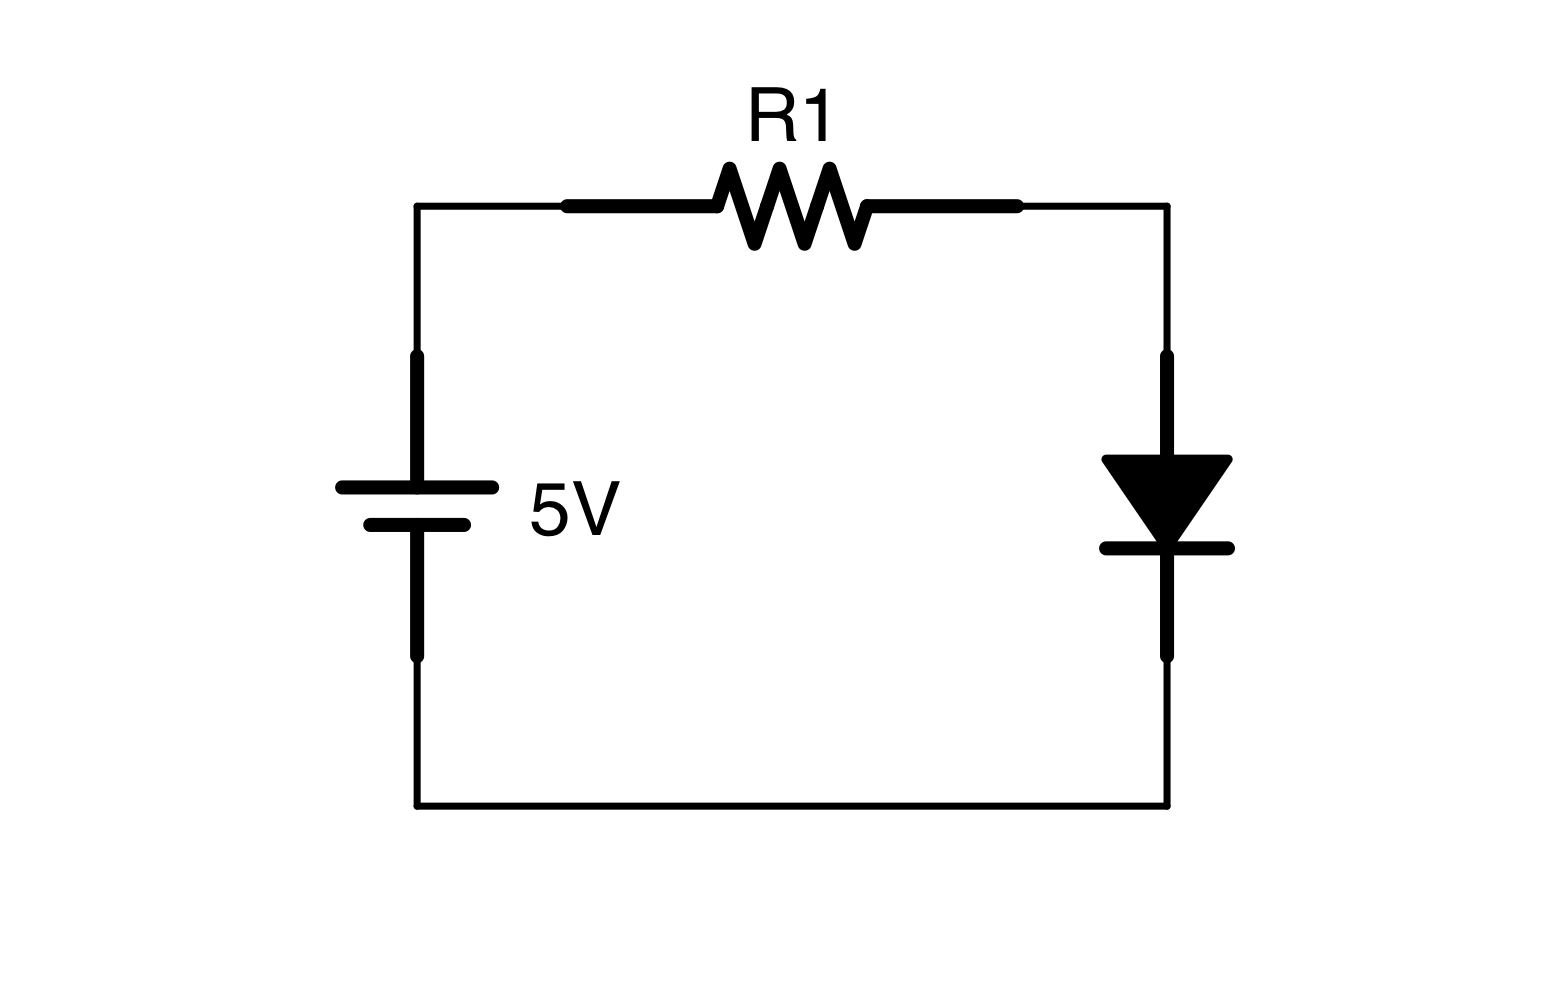
\includegraphics[scale=0.08]{DiodeApplyEx1.png}
\item Let's say instead of a standard diode, the diode is a blue LED.  Recalculate the current going through each component and the voltage drops for each component.
\item In the circuit below, calculate how much current is flowing through each component and each component's voltage drop if R1 is $300\myohm$, R2 is $400\myohm$, and R3 is $500\myohm$.  \\ 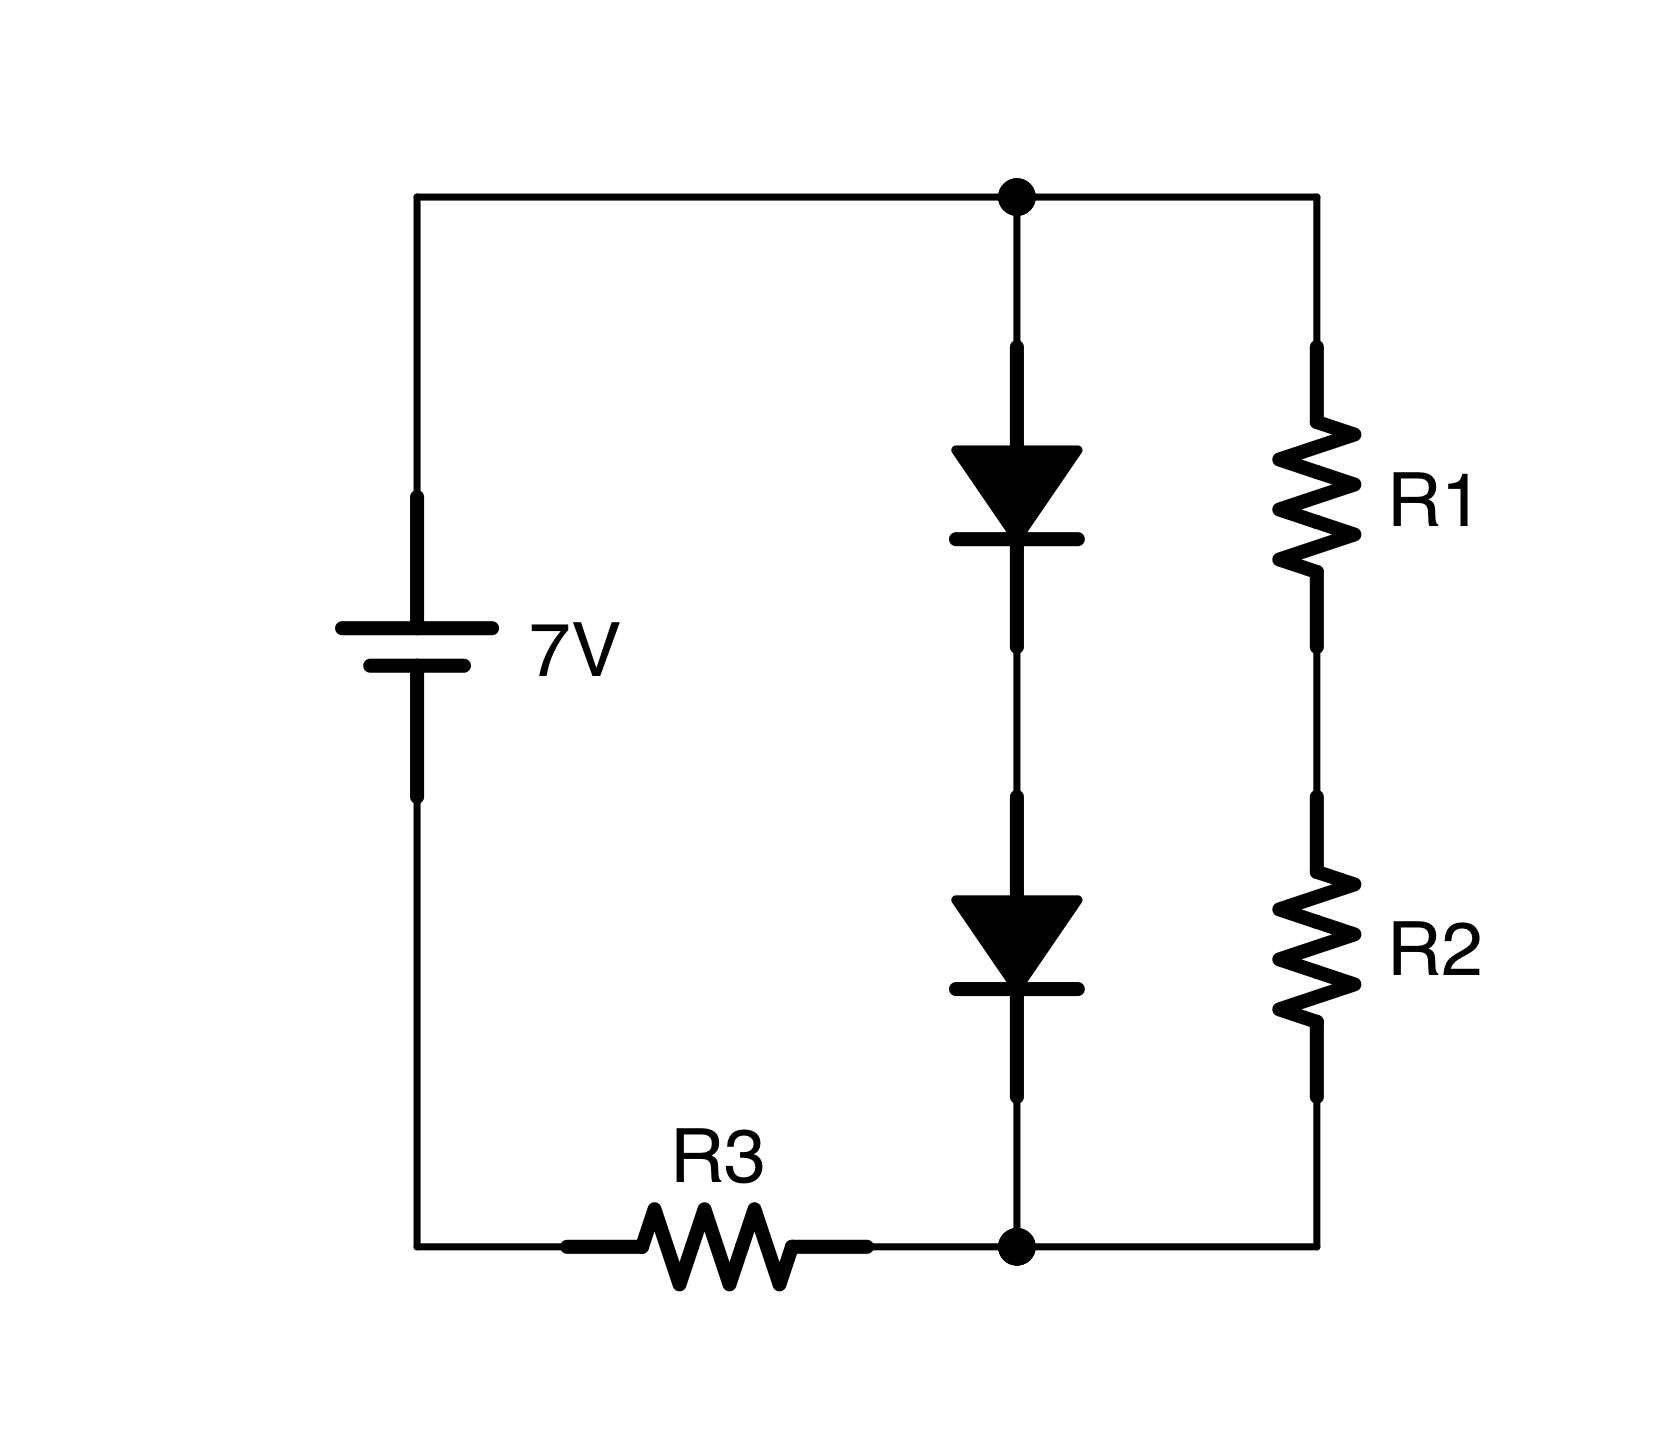
\includegraphics[scale=0.08]{DiodeApplyEx2.png}
\item Draw a circuit that provides a 6-volt regulated power supply to circuit load from a 9-volt battery using regular diodes.  Choose a resistor that works efficiently for a circuit load of $500\myohm$ and operates with a battery voltage from $7\myvolt$ to $9.6\myvolt$.  What is the current at the lowest and highest ranges of the battery?  How much is used by the circuit load and how much is wasted through the diodes in each configuration?
\item Draw an equivalent circuit to the previous question using a Zener diode instead of normal diodes.
\end{enumerate}

\chapter{Basic Resistor Circuit Patterns}
\label{chapBasicResistorCircuits}

When most people look at a schematic drawing, all they see is a sea of interconnected components with no rhyme or reason combining them.
However, most circuits are actually a collection of \glossterm{circuit patterns}.
A circuit pattern is a common way of arranging components to accomplish an electronic task.
Experienced circuit designers can look at a circuit and see the patterns that are being used.
Instead of a mass of unrelated components, a circuit designer will look at a schematic and perceive a few basic patterns being implemented in a coherent way.

In this chapter, we are going to learn three basic resistor patterns, and learn to work with switches as well.

\section{Switches and Buttons}
% FIXME - should I move this to another chapter that needs content?

Switches and buttons are very simple devices, but nonetheless we probably need to take a moment to explain them.
A switch works by connecting or disconnecting a circuit.
A switch in the ``off'' position basically disconnects the wires so that the circuit can't complete.
A switch in the ``on'' position connects the wires.

There are different types of switches depending on their operation.
The ones we are concerned with are called ``single pole single throw'' (SPST) switches, which means that they control only one circuit (single pole), and the only thing they do is turn it on or off (single throw).

\simplegraphicsfigure{Schematic Symbols for an SPST Switch (left) and an APST button (right)}{SwitchSchematicSymbols}{0.08}

Figure~\ref{figSwitchSchematicSymbols} show what the schematic symbols for an SPST switch and an SPST momentary switch (i.e., a button) look like.
As the drawing indicates, when the switch is open, the circuit disconnects.
When the switch closes, it connects the circuit.
While the switch holds its position stable (someone has to manually switch it back and forth), the button only connects the circuit \emph{while it is being pushed}.  
While the button is being pushed, the circuit is connect, but as soon as someone stops pushing the button, the circuit opens back up.

\simplegraphicsfigure{A Simple Switch Circuit}{SimpleSwitchCircuit}{0.08}

Figure~\ref{figSimpleSwitchCircuit} shows what a simple circuit with a switch looks like.
It is just like a normal LED circuit, but with a switch controlling whether or not electricity can flow.
Note that the switch is just as effective on the other side of the circuit.
If the switch was the last part of the circuit, it would be equally as effective.  
Remember, in order for current to flow, there must be a full circuit from positive back to negative.

\section{Current-Limiting Resistor Pattern}

The first resistor pattern we are going to learn is one that we already know---the current-limiting resistor pattern.
The idea behind this pattern is that a resistor is added to limit the amount of current that can flow through a device.
The size of the resistor needed depends on the size of the voltage source, the action of the device itself, and the maximum amount of current to allow.
Then, the resistor size needed can be calculated using Ohm's Law.

Many resistors are added to circuits to limit current flow.
At the beginning, we used resistors to make sure we didn't destroy our LEDs.
In Chapter~\ref{chapDiodes}, we used a resistor to limit the amount of current flowing through our voltage regulation circuit.

In many different circuits, we will need resistors to limit current for two different reasons---to avoid breaking equipment and to save battery life.
Oftentimes, we are actually choosing resistor values to accomplish both of these tasks.

If an LED breaks with $20\mymamp$, then we need a resistor big enough to keep the current that low.
However, if the LED light is sufficiently visible with $1\mymamp$, then, to save battery life, we might want a bigger resistor.
Battery capacity is often measured in milliamp-hours (mAh), with a typical $9\myvolt$ battery holding 400mAh.  
So, with such a battery, an LED circuit at $10\mymamp$ will drain the battery in 40 hours ($400\textrm{mAh} / 10\mymamp = 40\textrm{h}$), but the same LED circuit with a bigger resistor, limiting the current to $1\mymamp$ will take a full 400 hours ($400\textrm{mAh} / 1\mymamp = 400\textrm{h}$) to drain the same battery!
That will save you a lot of money in the long run.

\section{Voltage Divider Pattern}

\simplegraphicsfigure{A Simple Voltage Divider Circuit}{SimpleVoltageDivider}{0.08}

A \glossterm{voltage divider} occurs anytime there are two resistors together with a subcircuit coming out from in-between them.
They usually are connected to a fixed positive voltage on one side of the first resistor, and the ground on the other side of the second resistor, but this isn't strictly necessary.
A simple schematic of a voltage divider is shown in Figure~\ref{figSimpleVoltageDivider}.
Notice that there are two resistors between the voltage source and the ground (a 1k on top and a 2k on bottom) and a subcircuit (indicated by the load resistance) branching off from between them.
Under certain circumstances (which will be covered in a moment), we can basically ignore the parallel resistance of the subcircuit, and just look at the voltages at each point in the main voltage divider circuit.

We can see that the voltage at the top of the voltage divider is $9\myvolt$ (because it connects to the positive terminal) and at the bottom of the voltage divider it is $0\myvolt$ (because it connects to the negative terminal).  
Therefore, the total voltage drop across both resistors must be $9\myvolt$.
Since the resistors are in series (remember, we are ignoring the load for now), we can find the total resistance in the circuit by just adding their resistances.
So, $1,000\myohm + 2,000\myohm = 3,000\myohm$.
Since the current in a series is the same for the whole series, we can now use Ohm's Law to calculate the current flow:

$$ I = V / R = \frac{9\myvolt}{3,000\myohm} = 0.003\myamp = 3\mymamp $$

So, there is $0.003\myamp$ ($3\mymamp$) in this circuit.
That means that \emph{each} resistor in the series will have this amount of current flowing through them.
Therefore, we can calculate the voltage drop across each resistor.
Let's look at the 1k resistor:

$$ V = I * R = 0.003\myamp * 1,000\myohm = 3\myvolt $$

So, the voltage drop across the first resistor is $3\myvolt$.
That means that, since the battery started at $9\myvolt$, at the end of the resistor the voltage compared to ground is $6\myvolt$.
We can calculate the voltage drop across the second resistor either by Ohm's Law again or just by noting the fact that since the other end of the resistor is connected to ground, the voltage \emph{must} go from $6\myvolt$ to $0\myvolt$.

\simplegraphicsfigure{Voltage Divider with Voltages Labelled}{SimpleVoltageDividerLabelled}{0.08}

Figure~\ref{figSimpleVoltageDividerLabelled} shows the voltages at each point.
As you can see, the wire from the middle of the voltage divider has a new voltage that can be used by the load.
This is what voltage dividers are normally for---they provide a simple way of providing a scaled-down voltage to a different part of the circuit.

But how do we choose the values of the resistors?

One thing to note is that the second resistor consumed exactly twice as much voltage as the first resistor.
Additionally, the second resistor was exactly twice as large as the first resistor.
Thus, as a general principle, the relative sizes of the resistors will determine the relative amounts of voltage they eat up.
So, if we needed a $4.5\myvolt$ output, that is half of our input voltage.
Therefore, we would need both resistors to be the same.

A more explicit way of stating this is with an equation.
Given a starting voltage $V_{IN}$ connected to the first resistor, $R_1$, and the second resistor ($R_2$) connected to ground, the output voltage ($V_{OUT}$) coming out between the resistors will be given by the equation:

\begin{equation}
V_{OUT} = V_{IN} * \frac{R_2}{R_1 + R_2}
\end{equation}

Note that the specific values don't matter yet---it is the \emph{ratio} we are concerned about so far.
To get $4.5\myvolt$, we can use two $1\mykohm$ resistors, two $200\myohm$ resistors, or two $100\mykohm$ resistors.
As long as the values are the same, we will divide the voltage in half.

If we wanted an $8\myvolt$ output, we would do a similar calculation.  
Since we start at $9\myvolt$, we need to use up $\frac{1}{9}$ of the voltage in the first resistor, and $\frac{8}{9}$ of the voltage in the second resistor.
Therefore, our resistors need to be in similar ratio.
We could use an $100\myohm$ resistor for the first resistor, and a $200\myohm$ resistor for the second resistor.

So how do you determine exactly what value to use?
Here is where we start thinking about the load again.
While we have been treating the voltage divider as a series circuit, in truth we have one resistor in series, and then a parallel circuit with the other voltage divider resistor in parallel with the load.
Our simplified model (where we ignore the parallel resistance) will work, \emph{as long as the load resistance does not impact the total parallel resistance by a significant amount}.
Therefore, let's look at how the load resistance affects the parallel resistance.

So, using Equation~\ref{eqparallelresistancen} we can write a formula for the total resistance of these two, with $R_2$ being our second voltage divider resistor and $R_L$ being our load resistance:

$$ R_T = \frac{1}{\frac{1}{R_2} + \frac{1}{R_L}} $$

Now, let's look back at the circuit in Figure~\ref{figSimpleVoltageDividerLabelled}.
Let's say that the resistance of the load ($R_L$) is $400\myohm$, which is much less than the resistance of the voltage divider resistor ($R_2$).
So what is the total resistance?

$$ R_T = \frac{1}{\frac{1}{R_2} + \frac{1}{R_L}} = \frac{1}{\frac{1}{2,000} + \frac{1}{400}} = \frac{1}{0.0005 + 0.0025} = \frac{1}{0.003} \approx 333\myohm $$

This is way off of our simplified model which ignored the load resistance, which gave $2,000\myohm$.
Now, let's increase the load resistance so that it is equal to the load resistance ($2,000\myohm$) and recalculate:

$$ R_T = \frac{1}{\frac{1}{R_2} + \frac{1}{R_L}} = \frac{1}{\frac{1}{2,000} + \frac{1}{2,000}} = \frac{1}{0.0005 + 0.0005} = \frac{1}{0.001} \approx 1,000\myohm $$

This is still significantly off, but it is much closer.
So, now, let's look at what happens if the load resistance is double of $R_2$, or $4,000\myohm$:

$$ R_T = \frac{1}{\frac{1}{R_2} + \frac{1}{R_L}} = \frac{1}{\frac{1}{2,000} + \frac{1}{4,000}} = \frac{1}{0.0005 + 0.00025} = \frac{1}{0.00075} \approx 1,333\myohm $$

Here, we are getting much closer to our original value.  Now, let's say that the load is ten times the resistance of our $R_2$ resistor, or $20,000\myohm$.  That give us this:

$$ R_T = \frac{1}{\frac{1}{R_2} + \frac{1}{R_L}} = \frac{1}{\frac{1}{2,000} + \frac{1}{20,000}} = \frac{1}{0.0005 + 0.00005} = \frac{1}{0.00055} \approx 1,818\myohm $$

This is very close to the resistance of $R_2$ by itself.
So, what we can say is that our voltage divider circuit can ignore the resistance of the load \emph{if the resistance of the load is significantly more than the resistance of the voltage divider resistor}.
A way of writing this down is that $R_L >> R_2$.
What ``significantly'' means depends on how sensitive your circuit it to voltage changes, but, generally, I would say that $R_L$ should be at least ten times $R_2$.

So, for low-resistance loads, a voltage divider does not work well, because it puts too little resistance between the voltage source and ground.
However, in Chapter~\ref{chapIC} we will see that many circuit have loads of approximately infinite resistance, so voltage dividers work well.

In general terms, a voltage divider with smaller resistors is ``stiffer'' because it varies less in response to variations in a load, but it also eats up more current.
A voltage divider with larger resistors doesn't work with low-resistance loads, but it also uses up much less current.

\section{The Pull-Up Resistor}
\label{secPullUpResistor}

The pull-up resistor is a strange circuit, but we will find very good applications for it once we start dealing with ICs in Chapter~\ref{chapIC}.
It is probably easiest to describe by simply showing you a circuit and then describing how it works.

\simplegraphicsfigure{Basic Pull-Up Resistor}{PullUpResistorBasic}{0.08}

Figure~\ref{figPullUpResistorBasic} shows the circuit diagram for a basic pull-up resistor circuit.
Normally, we think of lighting up an LED by pushing the button.
However, in this case, pushing the button causes the current to bypass the LED.

If you look at the path from where the circuit branches, when the button is not pressed, the current can only go one way---through the LED.
However, when the button is pressed, the electricity has two options---either through the LED or directly to ground through the button.
The electricity would always rather go directly to ground rather than through an intermediary, so \emph{all} of the current goes through the closed button, and none of it goes through the LED.

Since the branch point is directly connected to ground when the button is pushed, that means that the voltage \emph{at the branch point} is also zero.
Kirchoff's Voltage Law says that no matter what path is taken, the voltage drop will always be the same.
However, an LED induces a voltage drop, but the voltages on both sides of the LED are zero.
Therefore, electricity cannot flow through the LED.

So what is the function of the resistor?
The resistor connects the switch and the LED to the positive voltage source, and provides a limitation on the current that runs through it.
The resistor must be \emph{before} the branch point for it to work.

Think about what happens without the resistor, or if the resistor is after the branch point.
The electricity will have a path directly from the positive voltage source to ground with no resistance---in other words, a short circuit.
This will draw an enormous amount of electricity.
Figure~\ref{figPullUpResistorBad} shows what this would look like.
Notice that when the button is pushed, you can trace a path from the positive voltage source to ground with no intervening resistance.

\simplegraphicsfigure{Incorrect Way to Wire the Circuit}{PullUpResistorBad}{0.08}

The resistor is called a pull-up resistor because it is connected to the positive voltage source, and is used to ``pull up'' the voltage on the circuit to a positive value when the switch is open.
In Chapter~FIXME we will look at resistors that are connected to ground, called pull-down resistors.

In short, a pull-up resistor is usually used to supply positive voltage to a circuit which might be turned off by redirecting the voltage to ground.
The resistor provides both the electrical connection to the positive source and a limit to the amount of current that will flow if the wire is then routed to ground (usually through some kind of switching mechanism).

\reviewsection

In this chapter, we learned:

\begin{enumerate}
\item Most circuits are a combination of common, well-understood circuit patterns.
\item The more experienced you are with circuits, the easier it is to see these circuit patterns when you look at a schematic drawing.
\item A current-limiting resistor is a resistor that is used to limit the maximum current flow within a circuit, either to protect other components or to limit overall electricity usage.
\item A voltage divider is a pair of two resistors connected in series with one another (usually connected to a positive voltage on one side and the ground on the other), but with another wire coming out in-between them to provide voltage to another circuit (called the \emph{load}).
\item In a voltage divider, it is assumed that the resistance of the load is significantly more than the resistance of the second half of the voltage divider because then the load can be basically ignored for calculating voltage drops.
\item For a voltage divider, the ratio of the voltages consumed by each resistor is the same as the ratio of their resistances.  The output voltage coming out between them is the same as the voltage used by the second resistor.
\item Another way of stating the output voltage is $V_{OUT} = V_{IN} * \frac{R_2}{R_1 + R_2}$, where $R_1$ is the resistor connected to the positive voltage and $R_2$ is the resistor connected to ground.
\item Voltage dividers with smaller resistances are ``stiffer''---they are impacted less by the resistance of the load.  Voltage dividers with larger resistances waste much less current.
\item A pull-up resistor circuit is a circuit in which a positive voltage which may be switched to ground at some point is provided through a resistor.
\item The pull-up resistor both (a) connects the circuit to the positive voltage to supply a positive current when the circuit is not switched to ground and (b) limits the current going to ground (i.e., prevents a short circuit) when the load is switched to ground.
\item It is called a pull-up resistor because it pulls the voltage up when the circuit is not switched to ground.
\end{enumerate}

\applysection

\begin{enumerate}
\item Given a $15\myvol$ voltage supply, what size of a resistor would be needed to make sure that a circuit never went over $18\mymamp$.
\item Given a $9\myvolt$ battery source, design a voltage divider that will output $7\myvolt$ to a load that has a resistance of $10\mykohm$.
\item Given a $3\myvolt$ battery source, design a voltage divider that will output $1.5\myvolt$ to a load that has a resistnace of $1\mykohm$.
\item In Figure~\ref{figPullUpResistorBasic}, how much current is going through the circuit when the switch is open?  How much when it is closed?
\item How would you modify the circuit in Figure~\ref{figPullUpResistorBasic} to keep the maximum current in the circuit under $2\mymamp$?
\end{enumerate}

\chapter{Understanding Power}
\label{chappower}

So far we have covered the basic ideas of voltage, current, and resistance.
This is good for lighting up LEDs, but for doing work in the real world, what is really needed is \glossterm{power}.
This chapter on its own adds very little to your capabilties as a circuit designer, but it is absolutely critical background information for the chapters that follow.
Knowing about power, power conversions, and power dissipation will be critical to taking your electronics abilities into the real world.

\section{Important Terms Related to Power}

To understand what power is, we need to go through a few terms from physics (don't worry---they are all easy terms):

\begin{enumerate}
\item \glossterm{Work} happens when you move stuff.  
\item Work is measured in \glossterm{joules}. A joule is the amount of work performed when a 1 kilogram object is moved 1 meter.
\item The capacity to perform work is called \glossterm{energy}.  Energy is also measured in joules.
\item \glossterm{Power} is the sustained delivery of energy to a process.  
\item Power is measured \glossterm{watts} (abbreviated W).  Watts are just the number of joules per second.
\item Another measurement of power is horsepower (abbreviated hp).  1 horsepower is equivalent to 746 watts.  Horsepower is not important for electronics, but I wanted to mention this because horsepower is a term you have probably heard, and I wanted you to be able to connect its importance.
\end{enumerate}

One of the interesting things about work, energy, and power is that they can take on a number of forms that are all equivalent.
For instance, we can have mechanical energy, chemical energy, and electrical energy (as well as others).
We can also perform mechanical work, chemical work, and electrical work.
All these types of energy and work can be converted to each other.
They are all also measured in joules.
Therefore, we have a common unit of energy for any sort of task we want to accomplish.

Now, when we actually apply energy to perform work, we do not get a 100\% conversion rate.
That's because the process of conversion is \glossterm{inefficient}---not all of the energy gets directed to the task we want to perform.
There is no perfectly efficient process of converting energy to work.
Additionally, there is no way to create energy from nothing---any time you need additional energy you will need a source for it.

When energy is converted to work, \emph{all} of the energy does something, even if it isn't work on the task you want.
Usually, the inefficiencies get converted to \glossterm{heat}.
So, if I have a process that is only 10\% efficient, and I give that process 80 joules of energy, then that process will do only 8 joules of work, leaving 72 joules of energy that is converted to heat.

Work and energy are usually used for systems that do one thing and then stop at the end.
In electronics, we are usually building systems that stay on for long periods of time.
Therefore, instead of measuring energy, we measure power, which is the continuous delivery of power (or usage of power in doing work).

As we mentioned, power is measured in watts, which is 1 joule per second.
So, if you have a $100\mywatt$ light bulb, that bulb uses 100 joules of energy each second.
$100\mywatt$ light bulbs are very inefficient, which is why they get so hot---the energy that is not converted to light gets converted to heat instead.

\section{Power in Electronics}
\label{secpowerelec}

So, we have a basic idea about what power is in general.
In electronics, there are a few equivalent ways of calculating power.

The first is to multiply the number of volts being consumed by the number of amps of current going through a device:

\begin{equation}
P = V\times I
\end{equation}

Here, $P$ indicates power measured in watts, $V$ indicates volts, and $I$ indicates current measured in amps.
So, if my circuit is on a 9-volt battery, and I measure that the battery is delivering $20\mymamp$ to the circuit, then that means I can calculate the amount of power that my circuit is using (don't forget to convert milliamps to amps first!):

\begin{align*}
W &= V\cdot I \\
  &= 9\myvolt\cdot 20\mymamp  \\
  &= 9\myvolt\cdot 0.02\myamp \\
  &= 0.18\mywatt
\end{align*}

So, our circuit uses 0.18 watts of power.

You can also measure the amount of power that individual components use.
For instance, let's say that a resistor has a $3\myvolt$ voltage drop and has $12\mymamp$ of current running through it.
Therefore, the resistor uses up $3 * 0.12 = 0.36$ watts of power.

The second way of calculating power comes from applying Ohm's law.
Ohm's law say:

\begin{equation}
V = I\cdot R
\end{equation}

So, if we have the equation $P = V\cdot I$, Ohm's law allows us to \emph{replace} $V$ with $I\cdot R$.
Therefore, our new equation becomes:

\begin{equation}
P = (I\cdot R)\cdot I
\end{equation}

Or, we can simplify it further and say that

\begin{equation}
\label{eqpowercurrent}
P = I^2\times R
\end{equation}

We can also substitute $I = V / R$ and wind up with a third equation for power:

\begin{equation}
\label{eqpowervr}
P = V^2 / R
\end{equation}

So, if we have $15\mymamp$ running through a $200\myohm$ resistor, then we can calculate the amount of power being used using Equation~\ref{eqpowercurrent}:

\begin{align*}
W &= I^2\cdot R \\
  &= (15\mymamp)^2\cdot 200\myohm \\
  &= (0.015\myamp)^2\cdot 200\myohm \\
  &= 0.000225\cdot 200 \\
  &= 0.045\mywatt
\end{align*}

Now, if you think about it, the resistor isn't actually \emph{doing} anything.
It is just sitting there.
Therefore, since we are not accomplishing any \emph{work} by going through the resistor, the energy gets converted to heat.
Electronics components are usually rated for how much power they can \glossterm{dissipate}, or easily get rid of.
Most common resistors, for instance, are rated between $1/16\mywatt$ and $1/2\mywatt$ (most that I've seen for sale are $1/4\mywatt$).  
This means that they will continue to work as long as their power consumption stays under their limit.
If the power consumption goes too high, they will not be able to handle the increased heat, and will break (and possibly catch fire!).

So far, our projects have dealt with low enough power that this isn't a concern.  
In fact, using $9\myvolt$ batteries, it is hard to generate more than $1/4\mywatt$ of power---you would have to have less than $350\myohm$ of resistance on the \emph{whole} circuit, and have the entire voltage drop occur on the resistor.

\section{Handling Power Dissipation with Heat Sinks}

As we mentioned earlier, when power dissipates without doing any work, it is converted to heat.
Some devices need to dissipate large quantities of heat under regular workloads.
One common device that often needs to dissipate heat is the voltage regulator, like the 7805 regulator we encountered in Chapter~\ref{chapLogicICs}.

The way that this regulator performs its job is essentially by dissipating power until the voltage is at the right level.
When used with any serious amount of current, this can actually get very, very hot.
As such, the back side of these contains a metal plate which is used to dissipate heat.
Additionally, it has a metal tab with a hole that can be used to attach a \glossterm{heatsink}.

A heatsink is a metal structure with a large surface area that helps an electronic component dissipate heat.
By being made of metal, it quickly moves the heat into itself.
By having a large surface area, it can transfer the heat to the air, where it will then disperse into the environment.

\simplegraphicsfigure{}{heatsink7805}{.25}

Figure~\ref{figheatsink7805} shows a 7805 chip next to its heatsink.
To attach the heatsink, just screw it in to the 7805.
On the 7800 series of regulators, the tab is electrically connected to ground, so it should not produce a voltage.
However, other types of chips in the same TO-220 package may actually have a voltage on the tab. 
In such a case, it would be wise to buy an isolation kit to electrically isolate the chip from the heatsink, otherwise incidental contact with the heatsink could cause a short circuit.

\section{Transforming Power}

As we have discussed, energy (and therefore power) can be transformed among a variety of forms---mechanical, electrical, chemical, etc., as long as weremember that energy is only reduced or lost, never gained.
The essence of energy transformation is at the heart of what makes batteries work.
A battery contains energy stored in a chemical form.
Chemical reactions in the battery allow electrons to move.
By drawing the electrons through a specific path (drawing them to the positive from the negative), this reaction generates electrical energy.
So we have a conversion from chemical energy (the reaction of the chemicals in the battery) into electrical energy (the pull of the electrons through the circuit).

This can also go the other way.
Electrical energy can be used to stimulate chemical reactions.
A common one is the separation of water into hydrogen and oxygen.

It is the same with mechanical energy.
In an electric motor, electrical energy is converted into mechanical energy in the motor.
But the reverse also can occur.
A power generator is made by converting mechanical energy into electrical energy.

We won't go into details on how each of these transformations work (you would need to take courses in chemistry, mechanics, etc. to know more), but the essential ideas are that

\begin{enumerate}
\item energy and power can be transformed between a variety of forms,
\item these forms of energy can all be measured with the same measuring stick (joules), and
\item every energy transformation will lose (never gain) some amount of energy through inefficiencies.
\end{enumerate}

Power and energy are known as \glossterm{conserved quantities}, because, although they are transformed, they are never created or lost.
When we talk about power lost through inefficiencies, the power actually isn't lost in total, it is merely converted to heat.
You can think of heat as power that is applied in a nonspecific direction.

In Section~\ref{secpowerelec}, we noted that in electronics, the power (measured in watts) is determined by \emph{both} the voltage and the current---by multiplying them together.
Therefore, what will be conserved in electronics will not be the voltage or the current individually, but their product.
What this means is that we can, at least in theory, increase the voltage without needing a power gain, but at the cost of current.
Likewise, we can, at least in theory, increase the current without needing a power gain, at the cost of voltage.
In both of these cases, rather than transforming electrical power to another form of power altogether, we are transforming it into a different configuration of electrical power.

Devices that convert electrical power between different voltage/current configurations are known as \glossterm{transformers}.
A step-up transformer is one that converts a low voltage to a higher voltage (at the cost of current), and a step-down transformer is one that converts a high voltage to a lower voltage (but can supply additional current).

Technically, for DC circuits, these are usually known as \glossterm{DC-DC power converters} or \glossterm{boost converters} instead of being called transformers, but the same rules apply---the total number of watts delivered can never increase but the voltage can be converted up and down at the expense of the current.
Note that if you tried to wire a regular AC transformer to a DC power supply, it would not deliver any power at all---DC-DC converters work on very different principles than AC converters.

So, if I had a source of $12\myvolt$ and $2\myamp$, then I would have a $12\cdot 2=24\mywatt$.
Therefore, it may be possible to convert that to $24\myvolt$, but I would only be able to get $1\myamp$ of current ($24\cdot 1=24$).
However, I could drop the voltage to get more current.  
If I needed $4\myamp$, I could reduce the voltage to $6\myvolt$.
Also remember that in doing these transformations there is always some amount of power loss as well, but these calculations will give you what the maximum possiblities are.

The actual mechanisms that these devices employ for doing power conversions are outside the scope of this book.

\section{Amplifying Low-Power Signals}

Microcontrollers (like the ATmega328/P) are only capable of processing and generating low-power signals.
The ATmega328/P can only source up to $40\mymamp$ per pin, and only about $200\mymamp$ total across all pins simultaneously.
At $5\myvolt$, $40\mymamp$ would yield a maximum of $0.2\mywatt$.
Therefore, if you want to turn on a device that requires more power than that, you will need to \glossterm{amplify} your signal.

Now, as we discussed previously, you can't actually create more power out of nothing.
What you can do is, instead of trying to \emph{create} power, you can instead \emph{control} power.
We will discuss several specific techniques on how to do this over the next few chapters, but the essential idea is that you can amplify a signal by using a small signal to control a larger one.

Think about your car.
The way that you control your car is by taking a low-power signal, such as the gas pedal, and using it to control a high-power signal, such as the engine.
My foot is not directly powering the car.
My foot is merely using the pedals to tell another power source---the engine---how much of its energy it should move.
My foot doesn't actually interact directly with the engine at all, except as a valve to unleash or not unleash the power of the engine.

In the same way, since the output signals from the microcontrollers are low-power, instead of using these signals directly we will use the signals to control larger sources of power.
Devices which can do this include devices such as relays, optocouplers, transistors, op-amps, and darlington arrays.
We will cover more about amplification starting in Chapter~\ref{chapTransistorIntro}.

\reviewsection

In this chapter, we learned:

\begin{enumerate}
\item Work is what happens when you move stuff, and is measured in joules.
\item Energy is the capacity to do work and is also measured in joules.
\item Power is the sustained delivery of energy, and is measured in joules per second, also called watts.
\item Power can be converted to a number of different forms.
\item Converting power to another form or using it to do work always has inefficiencies, and these inefficiencies result in heat.
\item In electronics, power (in watts) is calculated by multiplying the voltage by the current ($P = V\cdot I$).  It can also be calculated as $P = I^2\cdot R$ or $P = V^2 / R$.
\item To calculate the power consumption of an individual component, use the voltage drop \emph{of that component} and multiply the current flowing through it.
\item Most components have a maximum rating for the amount of power they can safely consume or dissipate.  Be sure your components stay under that limit.
\item Some components can handle additional power dissipation by adding a heatsink, which will more effectively dissipate the excess heat into the air.
\item Power can be transformed into other types of power (mechanical, chemical, etc.), but can never go beyond the original amount of power.
\item Electrical power can also be transformed into different combinations of voltage and current, as long as the total power remains the same.
\item Components that do this transformation are called transformers for AC power, and DC-DC converters for DC power.
\item Because power cannot be created, the way that signals are amplified is by using a small power signal to control a larger power source.
\end{enumerate}

\applysection


\begin{enumerate}
\item If I have 50 joules of energy, what is the maximum amount of work I could possibly do with that amount of energy?
\item If I am using up 10 joules of energy each second, how many watts am I using up?
\item If I convert 30 watts of mechanical power into electrical power with 50\% efficiency, how many watts of electrical power are delivered?
\item If I have a circuit powered by a $9\myvolt$ battery that uses $0.125\myamp$, how many watts does that circuit use?
\item If a resistor has a $2\myvolt$ drop with a $0.03\myamp$ current, how much power is the resistor dissipating?
\item If a resistor has a $3\myvolt$ drop with a $12\mymamp$ current, how much power is the resistor dissipating?
\item If a $700\myohm$ resistor has a $5\myvolt$ drop, how much power is the resistor dissipating?
\item If a $500\myohm$ resistor has $20\mymamp$ flowing through it, how much power is the resistor dissipating?
\item In the circuit below, calculate the voltage drop, current, and power dissipation of every component (except the battery). \\ 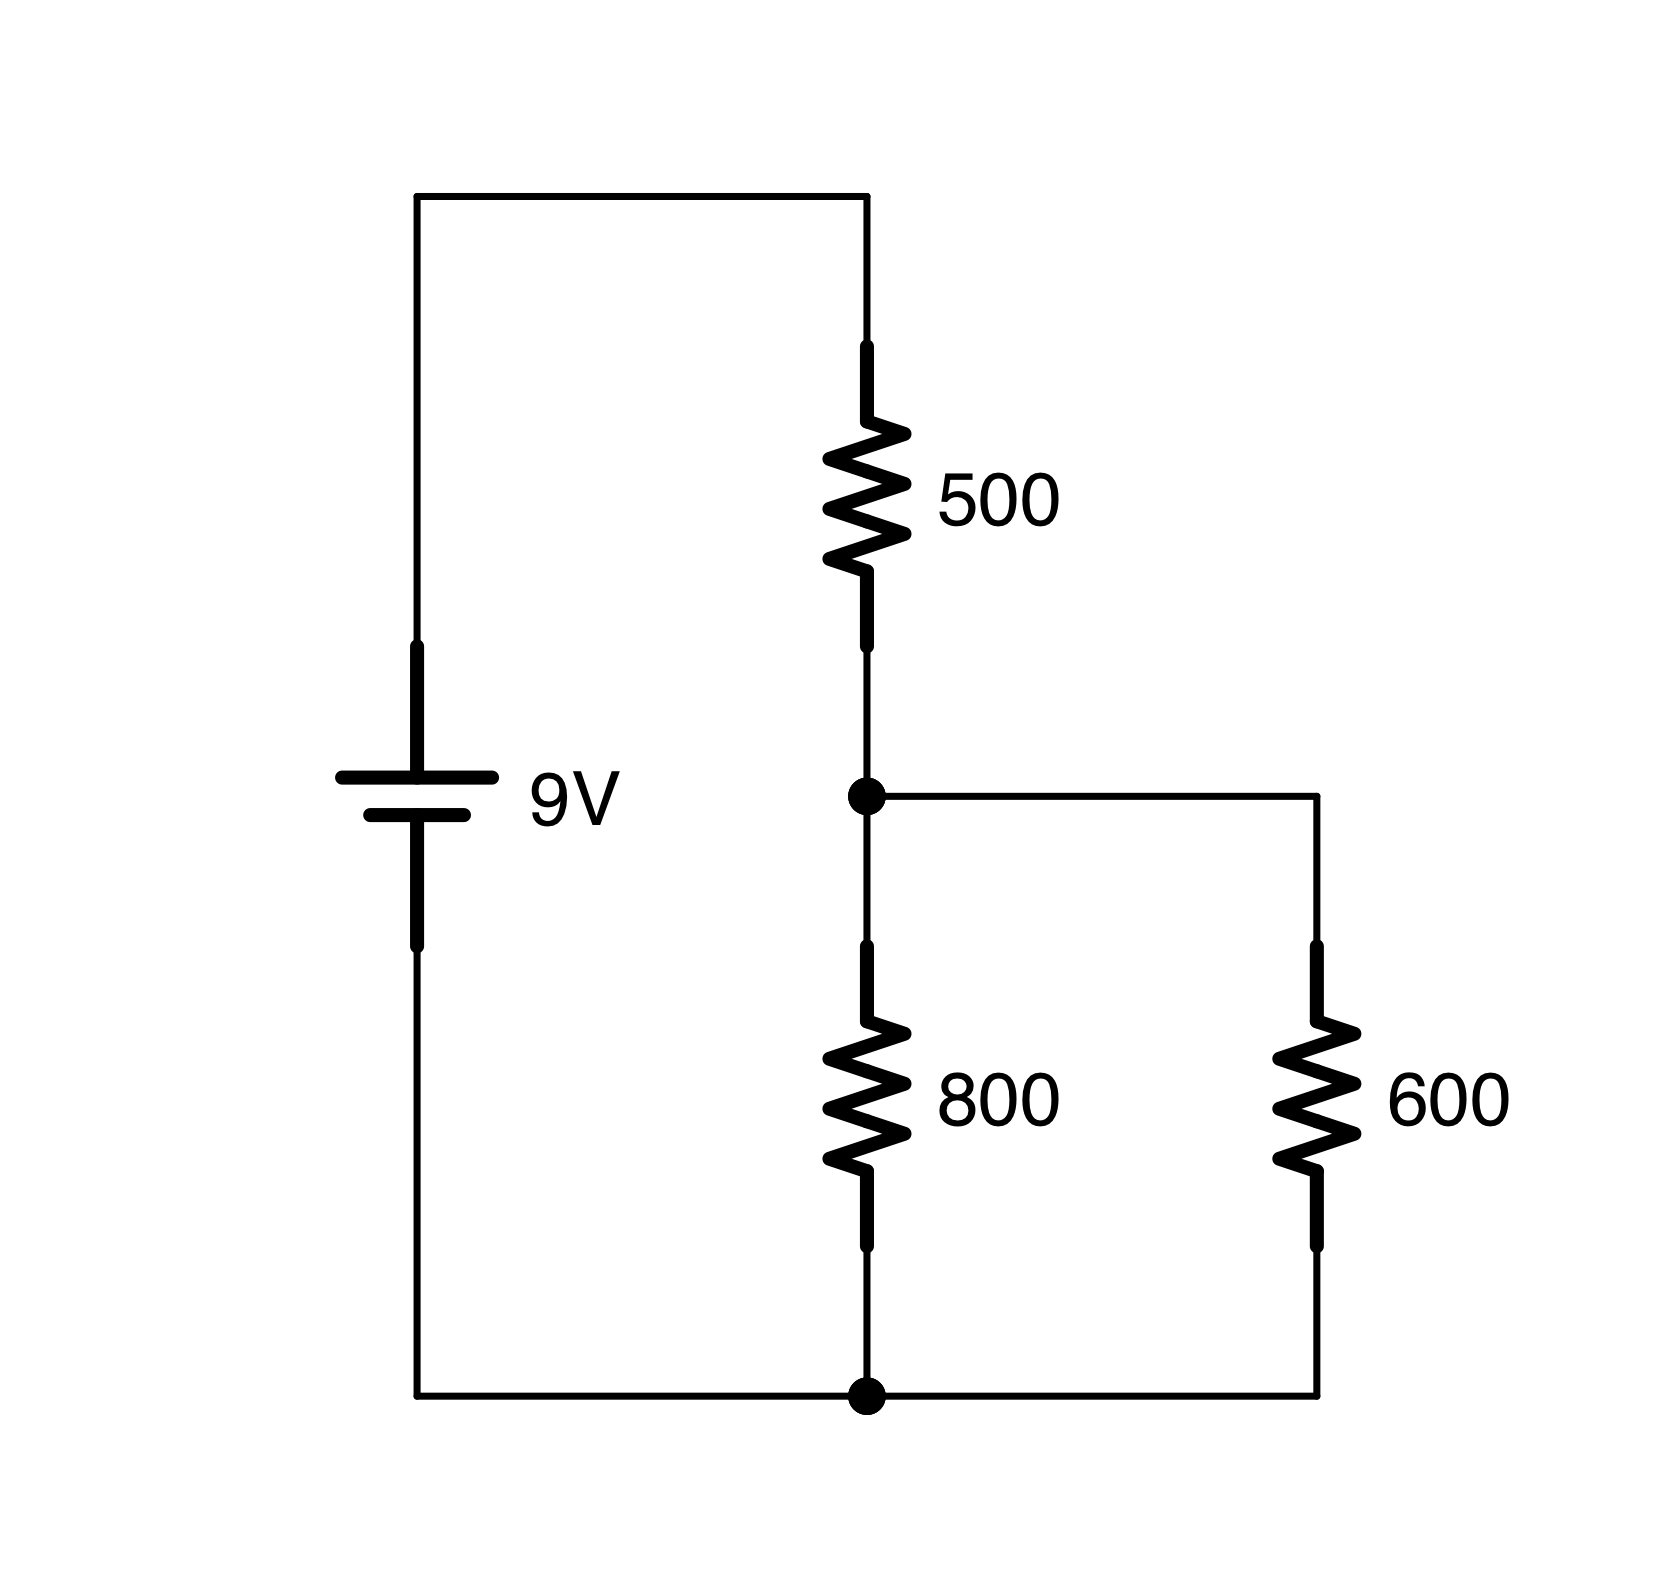
\includegraphics[scale=0.08]{ExampleForPowerDissipation.png}
\end{enumerate}



\part{Digital Electronics}

\chapter{Integrated Circuits and Resistive Sensors}
\label{chapIC}

So far, the components we have studied are simple, basic components---batteries, resistors, diodes, etc.
In this chapter, we are going to start to look at \glossterm{integrated circuits}, also called \glossterm{chips}, \glossterm{microchips}, or \glossterm{IC}s.
An IC is a miniaturized circuit placed on silicon.
It is a whole collection of parts geared around a specific function.
These functions may be small, such as comparing voltages or amplifying voltages, or they may be complex, such as processing video or even complete computers.
A single chip may hold just a few components, or it may hold billions.

Miniaturized circuits have several advantages---they are cheaper to produce in mass, they use less power, and they take up less space in your overall circuit---all because they have a reduced area and use fewer materials.
These miniaturized circuits are what allowed for the computer revolution over the last century.

\section{The Parts of an Integrated Circuit}

Integrated circuits, as we have noted, are basically miniaturized circuits placed on a siliconplate, called the die.
This die is where all of the action of the integrated circuit takes place.

The die is then placed into a \glossterm{package}, which then provides connection points for circuit designers to interface with the IC.
These connection points are often called \glossterm{pins} or \glossterm{pads}.
Each pin on an IC is numbered, starting with pin 1 (we will show you how to find pin 1 shortly).
Knowing which pin is which is important, because most of pins on a chip each have their own purposes, so if you attach a wire to the wrong pin your circuit won't work, or you will destroy the chip.
Most packages are marked with the chip's manufacturer and part number.

There are many different types of packaging available, but there are two general types that are often encountered:

\begin{description}
\item[Through-Hole] In this packaging type, the connection points are long pins which can be used on a breadboard.  This type of packaging is easiest for amateur usage.
\item[Surface Mount]  In this packaging type, the connection points are small pads which are meant to be soldered to a circuit board.  This packages are much smaller (and therefore less expensive), and can be more easily managed by automated systems.  These are also referred to as SMD (surface mount devices) or SMT (surface mount technology).
\end{description}

\simplegraphicsfigure{Comparison of the Same IC in SMD (left) and DIP (right) Packages}{DIPAndSMD}{0.125}

Since we are only using breadboards in this book and not doing any soldering, we will only concern ourselves with through-hole packaging.
However, through-hole packaging itself comes in a variety of styles.
The main one we will concern ourselves with is called a \glossterm{dual in-line package}, or \glossterm{DIP}.  

\simplegraphicsfigure{Pin 1 is Immediately Counterclockwise of the Notch}{FindPin1}{0.125}

An Integrated Circuit in a DIP package has two rows of pins coming out of the package.
Most chips mark either the top of the chip with a notch or indentation (where pin 1 is immediately counterclockwise of the notch), or mark pin 1 with an indentation, or both. 
See Figure~\ref{figFindPin1} to see how to use the notch to find pin 1.
The rest of the pins are numbered counterclockwise around the chip.

\simplegraphicsfigure{A DIP IC Inserted Into a Breadboard}{ChipInBreadboard}{0.125}

The beauty of a DIP packaged IC is that it fits perfectly onto most breadboards.
Figure~\ref{figChipInBreadboard} shows how you can place your IC across the breadboard's bridge and each pin on the chip will have its own terminal strip to connect to.

Be careful, though, when inserting ICs into breadboards.
The pins on an IC are often slightly wider than the breadboard.
If you just jam the IC into the breadboard, you will likely accidentally crush one or more of the pins that aren't exactly aligned on the hole.
Instead, compare the width of the pins to the width it has to fit in on your breadboard.
If it doesn't match up, \emph{very gently} bend the pins with your fingers or with pliers to get them to match up.

Usually, the ICs that I purchase are just a little wide, and I will squeeze the pins on each side slightly between my thumb and finger until they move close enough together.
However, you adjust the pins, make sure they line up before pushing them into their connection points on the breadboard.
Also, with larger ICs, you may need to adjust the IC back and forth as you gently insert it into place on the breadboard.

\section{The LM393 Voltage Comparator}

There are thousands and thousands of available chips which do a dizzying array of functions.
In this chapter, we are going to focus on a very simple chip---the LM393 Voltage Comparator.
This chip does one simple task.
The LM393 compares two input voltages, and then outputs either a high-voltage signal or a low-voltage signal depending on which input voltage is greater.
The LM393 is actually a \emph{dual} voltage comparator, which means that it will do two separate comparisons on the same chip.
Like most chips, the LM393 is an \emph{active} device, which means that it additionally requires a voltage source and a ground connection to provide power to the device.

\simplegraphicsfigure{The Pin Configuration of an LM393}{lm393Pinout}{0.25}

Figure~\ref{figlm393Pinout} shows the pin configuration (also called the \glossterm{pinout}) of the LM393.
The first thing to note on any pinout is where the voltage and ground connections are.
In this case, the voltage is marked as $V_{CC}$ and the ground is marked as $GND$.
Even though the LM393 has \emph{two} voltage comparators on the chip, they both share the power ($V_{CC}$) and ground ($GND$) pins.
The left side of the chip diagram shows the inputs and output for the first voltage comparator ($1IN+$, $1IN-$, and $1OUT$), and the inputs and output for the second voltage comparator is on the right ($2IN+$, $2IN-$, and $2OUT$).
In your projects, you can use whichever one is more convenient for you, or even both at the same time.

So, the \icode{1IN+} pin (pin 3) and the \icode{1IN-} pins are where the two voltages are being fed that are being compared by the first comparator.
The \icode{1OUT} is the pin which will contain the output.
If the voltage at \icode{1IN+} is less than the voltage on \icode{1IN-}, the output pin will be at a low (i.e., zero/ground) voltage.
If the voltage at \icode{1IN+} is greater than the voltage on \icode{1IN-}, the output pin \emph{will not conduct at all}, but this will be considered a ``high'' (positive-voltage) state.
This sounds counterintuitive, but, as we will see, this lets us set our own output voltage to whatever we want without causing too much complexity.
This configuration where high-voltage outputs don't conduct is called an \glossterm{open collector} configuration.
Don't worry if this is a little confusing, we will discuss it more in-depth later in the chapter.

\begin{sidebar}[Voltage Sources on Integrated Circuits]
Note that the voltage pins on integrated circuits can be marked in a number of different ways.
The positive voltage source is often labelled as $V_CC$, $V_DD$, or $V_+$.
The ground connect is often labelled as GND, $V_EE$, $V_SS$, or $V_-$.
There are additional ways that these are labelled as well.
Finding the positive and ground connections for an IC should always be the first thing you do with them.
\end{sidebar}

\section{The Importance and Problems of Datasheets}

Every IC (and, usually, any other part as well) has a datasheet supplied by the manufacturer which tells you important details about how you should use their chip in your circuit.
Reading datasheets is one of the worst parts of electronics, in my opinion. 
For me, datasheets rarely have the information I am actually looking for in a way that is easy to find.

In fact, most datasheets assume that you already know how to use the device, and the datasheets are just there to supply additional details about the limitations of the device.
For instance, looking through the LM393 datasheet from Texas Instruments, the actual operation of the device isn't even listed until page 11, and there it is buried within a sub-subsection, almost as a side-note.

These datasheets are written by people who have spent a lot of time being electrical engineers, and they are written for people who have spent a lot of time being electrical engineers, so when mere mortals read the datasheets, the important pieces are often shrouded in unintelligible gibberish.
For instance, the fact that the ``high'' output state of the device doesn't conduct isn't mentioned explicitly anywhere at all in the datasheet.  
Instead, it is implied by the configuration.

The reason for this is that the datasheets are usually read by professionals familiar with the type of device, and just need to know the electrical details so they don't accidentally bend the device beyond the breaking point.
Thus, the datasheets oftentimes spend more time just showing and describing the layout of the circuit on the chip and graphs of different chip properties, and then you are left to interpret what that means for your circuit.
For advanced circuit designers, this is great.
For students and hobbyists, however, this is oftentimes more frustrating than helpful.

However, datasheets do often provide a few basic details that are helpful to everyone.
They will often tell you:
\begin{itemize}
\item What each pin does
\item What the power requirements are
\item What the outer limits of the chip's operation are
\item An example circuit that you can build with the device
\end{itemize}

For all of these reasons, Appendix~\ref{appSimplifiedDatasheets} contains simplified datasheets for a number of common devices that are easier to read than the standard ones. 

For the LM393, the important points are:

\begin{enumerate}
\item The input voltage on $V_{CC}$ can be anywhere between $2\myvolt$ and $36\myvolt$.
\item When sensing voltage, the LM393 doesn't really draw any (or at least much) current, so there are no parallel resistances we need to worry about.
\item The output is high when \icode{IN+} is greater than \icode{IN-}, and low (i.e., ground) when \icode{IN+} is less than \icode{IN-}, with an error range of about 2 millivolts.
\item When the output is low, the output pin will conduct current into itself (since it is at ground, positive charge will naturally flow into it), but if sink more than $6\mymamp$ into it, you will destroy it.
\item When the output is high, the device will not conduct any current.
\end{enumerate}

That isn't to say that the datasheets aren't important, but for a beginner the datasheets usually aren't what you need to get started.

\section{A Simple Circuit with the LM393}

In this section, I am going to show a simple circuit using the LM393 chip.
In doing so, we are going to be using several of the resistor circuit patterns that we learned in Chapter~\ref{chapBasicResistorCircuits}.

\simplegraphicsfigure{A Simple Comparator Circuit}{SimpleComparatorCircuit}{0.08}

The circuit we are discussing is shown in Figure~\ref{figSimpleComparatorCircuit}.
Can you identify the resistor circuit patterns?  
Take a minute and see if you can find some.
Note that the wire coming out of \icode{1IN-} crosses two wires that it is \emph{not} joined with.

The first thing to notice is that we have \emph{two} voltage dividers.
The first voltage divider is between R1 and R2.
Since R1 and R2 are the same resistance and are connected to both $9\myvolt$ and $0\myvolt$, that means that they divide the voltage in half, giving a $4.5\myvolt$ output.
The second voltage divider is between R3 and R4.
Since R3 is half of the resistance of R4, that means that it only uses up half as much voltage as R4.  
Thus, since R3 eats up $3\myvolt$ and R4 eats up $6\myvolt$, the wire coming out from the middle is at $6\myvolt$.

Then, to the right of the circuit, you can see that we have a current-limiting resistor in front of the LED.
That is not its only function, though.
It also functions, as we will see shortly, as a pull-up resistor.

So what is the big triangle?
Comparators (and several other circuits commonly placed on ICs) are represented as triangles in the schematic (we could have also placed the chip itself there).
Each of the connections are labelled the same as they are labelled in the pinout diagram in Figure~\ref{figlm393Pinout} so they would be easy to locate.

The way that the circuit works is very simple.
The voltage coming in to \icode{1IN+} is $6\myvolt$ and the voltage coming in to \icode{1IN-} is $4.5\myvolt$.
Since \icode{1IN+} is greater than \icode{1IN-} then that will turn \icode{1OUT} to high (positive voltage).
However, remember that we said that \icode{1OUT} \emph{does not conduct} when it is high.
It acts like an open switch.
Therefore, R5 acts like a pull-up resistor and supplies the positive voltage for us to our LED to turn it on.

Now let's say that the input voltages were reversed.
What would happen?
If \icode{1IN-} is greater than \icode{1IN+}, then \icode{1OUT} will go low (zero volts) and also conduct.
It will act like a closed switch going to ground.

Therefore, current will go the easy route - it will go through \icode{1OUT} (directly to ground) instead of through the LED ($1.8\myvolt$ or more).
This works just like the switch in the circuit in Section~\ref{secPullUpResistor}.
When \icode{1OUT} is low, it acts like a closed switch to ground.
When \icode{1OUT} is high, it acts like an open switch (and is whatever positive voltage you supply yourself).

The resistor R5 does several jobs.
The first job is to act as a pull-up resistor. 
Remember that a pull-up resistor prevents the load to ground from going too high when the switch is closed.
Without the pull-up resistor, when the switch is closed (\icode{1OUT} goes low), we would have a short-circuit from the voltage source to ground.
This would not only waste a large amount of electricity, it would break the LM393, because it can only sink a maximum of $6\mymamp$ of current.
Having a $3\mykohm$ resistor, we limit the current for the closed switch to $I = V / R = 9 / 3,000 = 0.003A = 3\mymamp $.

When the switch is open, the current flows through the resistor to the LED, and then the resistor acts as a current-limiting resistor for the LED.
The amount of current to the LED will be calculated as $I = V / R = (9 - 1.8) / 3,000 = 7.2 / 3,000 = 0.0024\myamp = 2.4\mymamp$.

\section{Resistive Sensors and Voltages}

One of the more practical uses of the voltage comparator circuit is to measure the values of sensors which act as variable resistors.
Many different materials in the world act as resistors.
What's really interesting is that many of these materials \emph{change their resistance} depending on external factors.
Some of them change their resistance based on temperature, pressure, light, humidity, and any number of other environmental factors.

Now, changing resistance doesn't tell us much by itself.
If we put a resistor between a voltage source and ground, it will always eat up that voltage source.
However, if you use it in concert with a fixed resistor to make a voltage divider, you can then get the output voltage to vary based on the changes in resistance.

\simplegraphicsfigure{A Simple Resistor Sensor Circuit}{SimpleResistiveSensorCircuit}{0.08}

Figure~\ref{figSimpleResistiveSensorCircuit} illustrates this principle.
It is a simple voltage divider, where the top resistor is actually a photoresistor (a resistor that varies based on light) and the bottom resistor has a fixed resistance.
Thus, as the light varies, the top resistance will vary.
This will change the ratio between the top and bottom resistor, which will affect the output voltage.

To use this circuit, you will need to know the resistances of your photoresistor on the different conditions you are interested in.
I usually use the GL5528, which ranges from $10\mykohm$ in bright light to $1\myMohm$ in complete darkness.
However, depending on your specific photoresistor as well as the light conditions that you think of as ``light'' and ``dark,'' the resistance values that are relevant for light and dark will be different for you.
So, whatever photoresistor you use, it is worthwhile to measure the resistance using your multimeter in the different conditions you think of as light and dark.

\section{Sensing and Reacting to Darkness}

So far in the book, we have focused entirely on example circuits that didn't really do anything.
They lit up, they had voltage and current, but there wasn't much interesting that they were doing.
However, now, we finally have enough knowledge to start building circuits that \emph{do} something.

We have:
\begin{enumerate}
\item A way to generate a fixed voltage (using a voltage divider)
\item A way to generate resistances from real-world events (photoresistors and other resistance sensors)
\item A way to convert changes in resistances to changes in voltage (using a voltage divider with one fixed resistor)
\item A way to compare our varying voltage to our fixed voltage (using the LM393 comparator)
\item A way to utilize the output signal from the LM393 to do work (using the pull-up resistor and the LED)
\end{enumerate}

There are a lot of pieces to put together this simple circuit, which is why it has taken so long to do anything worthwhile. 
However, if you have followed along carefully, now that you are here you should be able to see how all of this fits together.

What we will do is to take the circuit given in Figure~\ref{figSimpleComparatorCircuit} and modify R4 to be our photoresistor and R3 to be a fixed resistor.
In my own testing, I discovered that the light/dark switchover point for my photoresistor was about $15\mykohm$.
Therefore, I am going to use a $15\mykohm$ resistor as the fixed resistor for R3.
Yours may need to vary based on your experimentation with your photoresistor.

When the light is on, my photoresistor will have a lower resistance than $15\mykohm$, which will make the fixed resistor R3 use up more of the voltage.  
Thus, the voltage at the divider will be less than $4.5\myvolt$, which will turn \icode{1OUT} to low (which closes the switch and makes a path to ground on the output before it gets to the LED, which turns the LED off).

In low-light conditions, the resistance will jump way up above the resistance of the fixed resistor.
If the upper, fixed resistor has less resistance than the bottom resistor, then the voltage at the divider will be larger than $4.5\myvolt$, activating the comparator and turning \icode{1OUT} to high (i.e., opening the switch and allowing power to flow through the LED).

The final circuit is given in Figure~\ref{figDarknessSensorCircuit}.
You can see a way to lay it out on the breadboard in Figure~\ref{figDarknessSensorBreadboard}.

\simplegraphicsfigure{Darkness Sensor Schematic}{DarknessSensorCircuit}{0.08}

\simplegraphicsfigure{Darkness Sensor Breadboard Layout}{DarknessSensorBreadboard}{1}

\section{Sources and Sinks}

Two terms that often come up when dealing with circuits are the concepts of a current \glossterm{source} and a current \glossterm{sink}.
A source is a component whose pins might provide current to other parts of the circuit.
A sink is a component whose pins might pull current from other parts of the circuit.

For the LM393, its input pins neither source nor sink current (at least not any significant amount).
The input pins more-or-less just sense the voltage without pulling any measurable current.
Therefore, they are neither sources nor sinks of current.
Technically, they probably sink a few nanoamps (billionths of an amp), but not nearly enough to affect our circuit analysis.

The output pin, even though it is called an \emph{output}, doesn't source any current.  
Instead, it acts either as a sink (when low) or as a disconnected circuit (when high).
This is known as an \glossterm{open collector} output.

Anytime an IC sources or sinks current, be sure to read the datasheets on the maximum amount of current it can source or sink.
These are usually quantities that \emph{you} have to limit---they are merely telling you at what point their circuit will physically break.
Therefore, you must use resistors to limit the currents to make sure that they are within limits.

However, be aware that many (but certainly not all) ICs do not source current, using open collectors for their output operations.
This has the disadvantage that you have to supply your own voltage and pull-up resistor to the output pin, but it also has the advantage that the output is set to \emph{whatever voltage level you choose}.
In other words, you don't need to pick a new comparator IC to get a different output voltage.

\reviewsection

In this chapter, we learned:

\begin{enumerate}
\item Integrated Circuits (called ICs or chips) are miniaturized circuits packaged up into an a single chip that can be added to other circuits.
\item ICs can have a few or several billion components on them, depending on the function.
\item ICs have different types of packages, including through-hole (optimized for breadboards) and surface mount (optimized for soldering and machine placement).
\item Dual In-line Packages (DIP) are the most common through-hole packaging type used for students, hobbyists, and prototype-builders.
\item DIP chips should be placed in the breadboard saddling the bridge, so that each IC pin is attached to its own terminal strip.
\item On most chips, pin 1 is located immediately counterclockwise of the notch in the chip, and remaining pins are numbered counterclockwise.
\item Most ICs are active devices, meaning that they have a direct connection to a power supply in addition to their input and output pins.a
\item An ICs Datasheet is a document that tells about the electrical characteristics of an IC.  However, most of them are difficult to read and assume you are already familiar with the part.  However, they are very useful for getting a pinout for the chip as well as telling the maximum ratings for voltages and currents.
\item The LM393 is a dual voltage comparator IC---it compares two voltages and alters its output based on which is larger.
\item The LM393's inputs do not consume any significant current on them when sensing the input voltages.
\item The LM393's outputs are open collectors---which means that they act as a switch to ground.  When the output is ``low'' the pin acts as a closed switch to ground.  When the output is ``high'' the pin acts as a disconnected circuit.
\item Because the LM393 acts as a disconnected circuit when high, a pull-up resistor circuit is required to get an output voltage.
\item Many sensors are based on the fact that the resistance of many materials will change with environmental factors.  Therefore, the sensor acts as a variable resistor, with the resistance telling you about the environment.
\item A resistive sensor can be used with a fixed resistor to make a variable voltage divider, essentially converting the resistance to a voltage.
\item By putting the resistive voltage divider in comparison with a fixed reference, we can use the LM393 comparator to trigger an output when the sensor crosses some threshold of resistance.
\end{enumerate}

\applysection


\begin{enumerate}
\item  Calculate the amount of current flowing through each element of the circuit in Figure~\ref{figSimpleComparatorCircuit}.  You can presume that the LM393 uses about $1\mymamp$ for its own operation, and that the LED is a red, $1.8\myvolt$ LED.  What is the total amount of current used by the circuit?
\item Take the circuit in Figure~\ref{figSimpleComparatorCircuit} and swap which voltage divider is attached to \icode{1IN+} and \icode{1IN-}.  Now calculate the total amount of current used by this circuit.
\item The Spectra Flex Sensor is a resistive sensor that changes its resistance when bent.  When it is straight, it has a resistance of $10\mykohm$.  When it is bent, it has resistances of $60\mykohm$ and above.  Draw a circuit that turns on an LED when the resistor is bent.  You may invent your own symbol for the flex sensor.
\item Build the circuit in Figures~\ref{figDarknessSensorCircuit} and~\ref{figDarknessSensorBreadboard}. 
\item If you wanted to wait until the room was even darker before the LED went on, how would you change the circuit?
\end{enumerate}


\chapter{Using Logic ICs}
\label{chapLogicICs}

% FIXME - introduce the concept of inverted and make it a glossterm

In Chapter~\ref{chapIC}, we worked with our first Integrated Circuit, the LM393 Voltage Comparator.  
In this chapter, we are going to look at other ICs and talk more about how they are named and used in electronics.

\section{Logic ICs}

One of the easiest class of ICs to use are the \emph{logic} ICs.  
A logic IC is a chip that implements a basic function of \glossterm{digital logic}.
In digital logic, electric voltages are given meanings of either ``true'' or ``false,'' usually with ``false'' being a voltage near zero, and ``true'' being a positive voltage (often between 3--5 volts).
These values are also referred to a 1 (for true) and 0 (for false), or HIGH (for true) and LOW (for false).
Then, the digital logic ICs implement logic functions that combine different signals (usually designated as A and B) and give an output signal (usually designated as Y or Q).

For instance, the \glossterm{AND} function will output a ``true'' (positive voltage) value if both of its inputs are true, and will output a ``false'' (near-zero voltage) value otherwise.  
In other words, if A \emph{and} B are true, Y is true.
As another example, the \glossterm{OR} function will output a ``true'' value if either of its inputs are true.
In other words, if A \emph{or} B are true, Y is true.
Figure~\ref{figTruthTable} shows the most common types of logic operations and how they work.

\begin{figure}
\caption{Common Logic Operations}
\centering
\label{figTruthTable}
\begin{tabular}{l | l | l| | l}
\textbf{Operation} & \textbf{A} & \textbf{B} & \textbf{Y} (output) \\
\hline
AND & false & false & false \\
AND & false & true & false \\
AND & true & false & false \\
AND & true & true & true \\
\hline
OR & false & false & false \\
OR & false & true & true \\
OR & true & false & true \\
OR & true & true & true \\
\hline
XOR & false & false & false \\
XOR & false & true & true \\
XOR & true & false & true \\
XOR & true & true & false \\
\hline
NOR & false & false & true \\
NOR & false & true & false \\
NOR & true & false & false \\
NOR & true & true & false \\
\hline
NAND & false & false & true \\
NAND & false & true & true \\
NAND & true & false & true \\
NAND & true & true & false \\
\hline
NOT & false & N/A & true \\
NOT & true & N/A & false \\
\end{tabular}
\end{figure}

As we have seen, AND yields a true result when both A and B are true and OR yields a true result when either A or B are true.
So what are the others?
\glossterm{XOR} is \emph{exclusive OR}, which means that it is just like OR, but is also false when both inputs are true.
\glossterm{NOR} is \emph{not OR}, which means that it is the exact opposite of OR.
Likewise, \glossterm{NAND} is \emph{not AND}, which means that it is the exact opposite of AND.
Finally, \glossterm{NOT} only has one input, and simply reverses its value.

Each digital logic function, when implemented in electronics is called a \glossterm{gate}.
The nice thing about building circuits with logic gates is that, rather than using math, you can build circuits based on ordinary language.
If you were to say, ``I want my circuit to output a signal if both button 1 \emph{and} button 2 are pressed,'' then it is obvious that you would use an AND gate to accomplish this.

\simplegraphicsfigure{The Pinout of a CD4081 Chip}{CD4081Pinout}{0.16}

Most logic gates are implemented in chips that contain multiple (often four) implementations of the same gate.
For instance, the CD4081 chip is a quad NAND gate chip.
The pinout for this chip is shown in Figure~\ref{figCD4081Pinout}
Note that it has a supply voltage pin (pin 14) as well as a ground pin (pin 7) to supply power to all the gates on the chip.
Each logic gate is numbered 1--4 and the inputs are labelled A and B with the output of Y.

To use the chip, you pick which one of the four gates you are going to use (it doesn't really matter which).
If we want to use Gate~1, then we put our inputs on 1A and 1B and then our output signal goes to 1Y.
Note that, unlike the IC from the last chapter, this logic gate has a powered output---it actually supplies voltage and current to drive a (small) output signal.

Logic gates are wired to expect relatively fixed, predefined voltages on their inputs, and output the same voltage levels.
They do not need current-limiting resistors for their inputs because the inputs themselves are usually high-resistance (i.e., $1,000,000--10,000,000\myohm$).
Because of the high resistance on the inputs, it also means that even if there is a resistor on the input, it will not affect the input voltage significantly (think of a voltage divider with $1,000\myohm$ for the first resistor and $10,000,000\myohm$ for the second resistor---the voltage will not change much after the first resistor).
It also means that the current going into the gate is essentially ignorable ($I = \frac{V}{R} = \frac{5}{10,000,000} = 0.0005\mymamp$).

For some logic chips, the input voltage is expected to be around $3.3\myvolt$ or $5\myvolt$, while as for others it is based on the supply voltage.
However, nearly all ICs are limited in how much current they can put out before they fry.  
This is usually somewhere in the range of $8--20\mymamp$, depending on the chip.
Because of this, if you use a logic gate to directly power a device (such as an LED), you probably will need a current limiting resistor to keep the output current down below these limits.

There are logic chips that have open collector outputs (like the LM393 from Chapter~\ref{chapIC}), but they are more rare because they are harder to use.

\simplegraphicsfigure{Example Circuit Using an AND Gate}{LogicGateExample}{0.08}

Lets say that we want to build a circuit which will turn on an LED if \emph{both} of two buttons are pushed at the same time.
Figure~\ref{figLogicGateExample} shows a circuit to accomplish this.
It has two buttons, one wired to 1A (pin 1) and one wired to 1B (pin 2).
The output 1Y (pin 3) then goes to an LED with a current limiting resistor.
You may wonder what the resistors attached to the buttons are doing.
Those will be explained in Section~\ref{secPullDownResistors}.

For most logic chips, the manufacturers recommend that unused inputs (but not outputs!) be connected to ground. 
This makes the chip more efficient in power consumption, but for simple projects like these it isn't really necessary.
If you wish to connect the unused inputs to ground then it is a better circuit design.

Note that the circuit shows a $5\myvolt$ source.
While the CD4081 is tolerant of a wide range of input voltages and would operate just fine at $9\myvolt$, many digital logic chips are not.
Many digital logic chips operate at pre-specified voltages, usually either $5\myvolt$ or $3.3\myvolt$.
Therefore, we will take a moment and look at how we can get an input source for a specific voltage.

\section{Getting a $5\myvolt$ Source}

So far in this book, however, we have mostly dealt with $9\myvolt$ batteries.
However, digital logic circuits often operate at lower voltages (usually $5\myvolt$ or $3\myvolt$).

Therefore, we need to find a way to convert a $9\myvolt$ source into a $5\myvolt$ source.
There are several options for doing this, all depending on your requirements and/or the supplies you have available to you.

One option is to build a simple $5\myvolt$ power supply using the knowledge you already have.
In Chapter~\ref{chapBasicResistorCircuits} we showed how to build a voltage divider to step down the voltage from a higher voltage source to a lower one.
Although not ideal, this could work fine for simple test circuits.
A better option would be to build the Zener diode voltage regulator that was shown in Chapter~\ref{chapDiodes} if you have a $5\myvolt$ Zener diode handy.

\simplegraphicsfigure{A 7805 Voltage Regulator in a To-220 Package}{TO220Pkg}{0.08}

Another option is to use a voltage regulator IC.
The LM7805 is a simple voltage regulator circuit you can use to convert a $9\myvolt$ voltage source (or higher--up to $24\myvolt$) into a $5\myvolt$ voltage source with minimal current loss.
It is itself an IC, though with a different kind of packaging than we've seen, known as a \glossterm{TO-220 package}.
You can see what this looks like in Figure~\ref{figTO220Pkg}.
On these packages, if you are reading the writing on the package, pin 1 (input voltage) is on the left, pin 2 (ground) is in the middle, and pin 3 (output voltage) is on the right.
Figure~\ref{figVoltageRegulatorLogicGate} shows what this looks like in a circuit diagram.

\simplegraphicsfigure{Logic Gate Circuit with a Voltage Regulator}{VoltageRegulatorLogicGate}{0.08}

\simplegraphicsfigure{Simple Way to Attach the LM7805 to Your Breadboard}{LM7805Breadboard}{1}

Figure~\ref{figLM7805Breadboard} shows how to attach the LM7805 regulator to your breadboard.
First, plug the regulator into your breadboard so that each pin is on its own terminal strip.
Next, plug the positive wire from the battery into the terminal strip with the voltage regulator's pin 1 and the negative wire from the battery to the negative/ground power rail on the breadboard.
Then, connect the voltage regulator's pin 2 (ground) to the negative/ground power rail. 
Finally, connect the voltage regulator's pin 3 (output voltage) to the positive power rail.
You now have a $5\myvolt$ supply!

Note that some LM7805s have pins that are too big for breadboards.
That's unfortunate, but they are pretty rare.  
As long as you buy from companies that target hobbyists, you are likely to get a component that will work well with breadboards.

Another option for $5\myvolt$ power is to use an add-on unit for your breadboard.
There are many full-featured power units available for use in standard breadboards (unfortunately, there is no standard name or part number for these units, so we will just call them \emph{breadboard power units}).
This type of unit plugs into the power rails of your breadboard, and can output either $5\myvolt$ (the logic voltage we are using here) or $3.3\myvolt$ (another popular logic voltage).
The breadboard power unit can take voltage from a variety of sources, including batteries (with a compatible plug), a wall outlet (with an appropriate adapter), or even with USB power (either from your computer or a wall charger).
To use the breadboard power unit, be sure the jumpers are set to the correct output voltage, and be sure to plug it in to your breadboard in the correct direction.  
There is also an on/off switch provided in most such units so that you don't have to wire one yourself.
The breadboard power unit has positive/negative markings, so be sure they line up with the positive/negative markings on your breadboard.

\fixme{Show a photo of the power unit}

For the rest of the book, if the schematic requests a voltage other than $9\myvolt$, feel free to use any of these methods to supply the proper power to your projects.

\section{Pull-Down Resistors}
\label{secPullDownResistors}

In Figure~\ref{figLogicGateExample}, we looked at the circuit diagram for a simple AND gate.  
We noted that each button had a resistor connecting it to ground, but we did not mention why.
In digital logic circuits, buttons and single-pole switches, when they are open, essentially disconnect the circuit.
Because the inputs are high-resistance inputs (i.e., they use very little current), simply disconnecting the input circuits is not always enough to turn them off!
Think of it this way---when you connect the circuit by pushing the button, the whole wire becomes positive.
When you let go of the button, the state of the wire has not changed.
Eventually the positive charge will drain out through the gate, but, since the input uses so little current, it will take a while for that to happen.
Therefore, we have to provide another path for the electricity to go when the button is not pressed.
Note that some logic chips actually supply pull-up resistors internally which make the inputs always positive when disconnected.  
In those cases, the pull-down resistor does essentially the same job, but is even more necessary than before.

These resistors are called pull-down resistors because, when the button circuit is not connected, they pull the voltage level down close to zero through the resistor.
The resistor is very important because, when the button is connected, it keeps the voltage high and limits the amount of current that leaks out across the resistor.
If you directly connected the button to ground without the resistor, then pushing the button would not raise the voltage because it is still directly connected to ground, and would therefore remain at zero volts.  
Having the resistor there makes sure that the voltage on the inputs remains high while the button is pressed, and bleeds off when the button is released.

In short, without a path to ground, when you let go of the button, the input could remain high.
However, without the resistor, pushing the button would cause a short-circuit.
Therefore, a pull-down resistor allows voltage to drain off quickly when the button is not pressed, but also prevents disasters and wasted current when the button is pressed.

The value of a pull-down resistor is usually somewhere between $1\mykohm$ and $10\mykohm$.  
Beyond $10\mykohm$ the actual function of pulling the voltage down to zero can be slowed down.  
Additionally, even above $4\mykohm$ it is possible to interfere with the actual logic operation of the chip.
Having a resistor below $1\mykohm$, however, means that you are just wasting current.

So, for any button-type input to a digital logic circuit (where the circuit is \emph{phyiscally disconnected} when the input is off), a pull-down resistor is needed to make sure that the input \emph{actually} goes low when the circuit disconnects.

\section{Combining Logic Circuits}

Logic chips that operate at the same voltage are very easy to combine together.
Let's say that you had three buttons that you wanted to monitor, and you wanted the light to come on if someone pushed either buttons 1 \emph{and} 2 together \emph{or} button 3 (or all of them).
To do that, you would need an AND gate and an OR gate.
Buttons 1 and 2 would be wired with the AND gate, and button 3 would be combined with the output of the AND gate through an OR gate.

\simplegraphicsfigure{Multiple Logic Gates Combined in a Circuit}{MultipleGates}{0.08}

Figure~\ref{figMultipleGates} shows what this looks like.
Since there are so many voltage/ground connections, the figure does not have an explicit battery drawn, instead it simply shows $+5\myvolt$ wherever it should connect to the voltage source, and a ground symbol wherever it should connect to the battery negative.
As you can see here, there are two logic ICs---the CD4081 having the AND gate and the CD4071 having the OR gate.
The output of the first AND gate is wired into one of the inputs of the OR gate.

This works because, unlike the LM393 (discussed in Chapter~\ref{chapIC}), these logic gates actually supply output voltage and current as well.  
Because the inputs to the logic gates are high-resistance, there is no need for a current-limiting resistor when combining gates in this way.

Now, it is fine to draw logic circuits the way we have in Figure~\ref{figMultipleGates}.
However, as the logic becomes more complex, actually drawing all of the connections to voltage and ground become tiring, and trying to get all of the wires to the right spot on the chip can get messy as well.
Because of this, engineers have devised a simpler way of describing logic gates and logic circuits.

\simplegraphicsfigure{Logic Gates Represented as Shapes Instead of IC Pins}{MultipleGatesShapes}{0.08}

Instead of representing the entire chip on a schematic, engineers will represent only the logic gates themselves.
Additionally, since the power goes to the whole chip (and not the individual gates), in such a drawing the power connections for the gates are not shown.
The standard that was developed represents each type of gate with a shape.
Figure~\ref{figMultipleGatesShapes} shows what this circuit drawing looks like if it is drawn using shaped gates instead of IC pins.
The actual physical circuit is the same, this is only to simplify the schematics to make them easier to understand and follow.

\simplegraphicsfigure{Common Gates Used in Schematic Drawings}{CommonGates}{0.08}

Figure~\ref{figCommonGates} shows what these gate drawings look like.
The AND gate has a flat back panel and a simple, rounded front.
The OR gate looks a bit like a space shuttle, with both the back and the front angled.
The NOT gate is a triangle with a circle at the tip.
This circle can also be added to other gates to show that the gate is the opposite one.
For instance, a NAND gate is drawn by first drawing an AND gate, and then adding a circle to the front, indicating that the gate behaves like an AND gate with a NOT gate in front of it.
Similarly, the NOR gate is an OR gate with a circle in front of it.
The XOR gate is similar to the OR gate, but with an extra line going across its inputs.

Many times, the internal schematics of a chip are shown using gate symbols, in order to help you understand the operation of the chip and how the pins work.
For instance, Figure~\ref{figCD4081InternalLayout} shows how the CD4081 chip is wired up internally.
You can see the inputs going through the logic gate, and out towards the output.
While this isn't any new information you didn't already know, if may help you understand why the pins are laid out the way that they are.

\simplegraphicsfigure{The Internal Layout of the CD4081}{CD4081InternalLayout}{0.08}

As an interesting side-note, every logic function can actually be built from NAND gates, though you have to wire them up in strange ways.
You can actually build a computer entirely from NAND gates if you wanted to.
It is not incredibly important, but Figure~\ref{figNANDLogic} shows how to build each type of logic gate from NAND gates.
As an activity, go through the truth tables in Figure~\ref{figTruthTable} and see if you can follow how each set of values becomes the result.

\simplegraphicsfigure{How Each Gate Can Be Built from NAND Gates}{NANDLogic}{0.08}

\section{Understanding Chip Names}

One of the biggest problems in learning to build electronic devices is the bewildering array of chips, each with some weird name.
``Oh, for that you want an NE555P,'' or, ``You could use a SN74HC00P or a CD4011BE for that task.''
What language are such people speaking?

There is a huge selection of chips available, and learning their names is a daunting task.
Appendix~\ref{appICNaming} attempts to offer some method to the madness, but, at the end of the day, chip names are like people's names---you get to know them by using them.
Nobody knows everybody's name, but, for the types of projects you like to work on (whatever that happens to be), there will be standard chips whose names you will eventually come to know.

Once you make it through this book, you should have a solid enough background to search for the chips you need, have some understanding of the part names, and be able to find the chips you need for your projects.
If you buy the chips from a seller geared towards amateurs and hobbyists, they will likely also include tutorials and additional information available in an easier-to-understand format than just datasheets.

% FIXME - refer questions to a forum

\reviewsection

In this chapter, we learned:

\begin{enumerate}
\item A logic IC implements basic digital logic functions such as AND, OR, NOT, etc.
\item These logic functions refer to essentially the same ideas that they mean in ordinary language, and exactly what they mean in formal logic.
\item Logic ICs use different voltage levels for true and false---usually with true being near the supply voltage and false being near zero voltage.
\item True is sometimes referred to as HIGH or 1.  False is sometimes referred to as LOW or 0.
\item The inputs of a logic function are usually designated as A and B, and the output is usually designated as Y or Q.
\item A single digital logic function is called a gate.  Most logic ICs have more than one gate on a single chip.
\item Logic ICs require a supply voltage and a ground connection to power the logic.
\item Most logic ICs provide powered logic outputs, so that a ``true'' value supplies both voltage and a small amount of current on its output.  However, a current-limiting resistor is usually required.
\item If an input to a logic IC may be disconnected for its ``false'' state (as is common with button inputs), then it needs a pull-down resistor to connect it to ground when the button is not being pushed.
\item Logic ICs can usually be combined by wiring the output of one to the input of another to create more complex logical conditions.
\item Logic gates are often drawn in schematics using basic shapes to indicate their operation, rather than as connections to chips.  In these cases, the power connections are not shown by schematics.
\item Every logic gate can actually be built from NAND gates wired together.
\item IC names are very confusing and take time and experience to get to know them well.
\item Many ICs require specific voltage levels to operate, often at $5\myvolt$ or $3.3\myvolt$.
\item Many solutions are available for generating specific voltages, including voltage dividers, zener diodes, voltage regulators, and add-on breadboard power units.
\item The LM7805 is a very common $5\myvolt$ voltage regulator.
\end{enumerate}

\applysection

\begin{enumerate}
\item Draw the circuit in Figure~\ref{figLogicGateExample} yourself.  Identify the function of each resistor.
\item Build the circuit in Figure~\ref{figLogicGateExample} (don't forget that the power source should be $5\myvolt$).
\item If you assume that no current flows through the inputs of the AND gate, and that the output functions as a $5\myvolt$ power source, how much current flows through each resistor when all of the buttons are pressed?  What, then, is the total current used by the circuit if you ignore the logic gate?
\item Measure the actual current that flows through each resistor.  If you are having trouble pushing the buttons while you measure the current, just replace the buttons with wires for this test.
\item Measure the current that it used by the AND gate itself.  You can do this by measuring the supply current of the AND gate.  Measure it both when its output is true and false.
\item Draw a schematic of a circuit that has two buttons (B1 and B2) which light up an LED if either button is pressed.
\item Draw a schematic of a circuit that has two buttons (B1 and B2) which light up an LED if neither button is pressed.
\item Draw a schematic of a circuit that has four buttons (B1--B4) which light up an LED if either B1 and B2 are pressed or if B3 and B4 are pressed.
\item Look at the construction of the different gates from NAND gates in Figure~\ref{figNANDLogic}.  Copy down the OR gate construction four times, and trace how the output is generated for each possible set of inputs (true/true, true/false, false/true, false/false).  Show the inputs and outputs on each NAND gate.  Compare the outputs to the truth table for the OR function in Figure~\ref{figTruthTable}.
\item Take the circuit in Figure~\ref{figLogicGateExample} and draw a schematic to use pull-up resistors on the inputs rather than pull-down resistors.  How will this change the behavior of the circuit?
\item Let's say that we want to create a door buzzer so that someone outside a door can push a button to be let in.  However, the person inside also wants a switch to be able to disable the buzzer.  The buzzer can be thought of as a simple device that buzzes when any positive voltage is applied.  Draw a circuit diagram of this setup using logic gates.  The buzzer can be drawn as a resistor labelled ``buzzer'' (don't forget to connect the other side to ground).
\end{enumerate}

\chapter{Using Logic Chips to Store Values}
\label{chapStorage}

\chapter{Common Integrated Circuits}

In Chapter~\ref{chapLogicICs} we studied basic logic circuits.
This chapter will introduce you to a few more complexi integrated circuits that are generally useful in a variety of applications.
Even more types of ICs can be found in Appendix~\ref{appSimplifiedDatasheets}.

\section{Holding a State}

Up until now, all of our circuits have fluctuated with their inputs. 
That is, the output is always determined by the \emph{present} state of the inputs.
But what happens if we want a circuit to \emph{remember} that something happened?
For that, we will need a way to set a state in the circuit and then hold it.
That is, we need something that we can tell it to remember a true/false value until we tell it not to.

Holding on to past states is called \glossterm{memory}.
In your computer you have huge memory chips that have billions of switches that can hold a state.
For our purposes, we will content ourselves to using chips that only hold a few states.

The simplest kind of memory in electronics is known as a \glossterm{latch}.
Latches hold a single \glossterm{bit} of memory.
A bit is simply a single true/false signal (i.e., positive voltage/zero voltage).
Latches allow you to store a true/false value and continue to retrieve it as often as you want until you choose to reset the value.
There are many different latches that are based on how they are set (and how complicated the circuitry is to implement them).

The easiest type of latch to learn about and use is the \glossterm{SR Latch}.
The SR Latch holds a value that it continually outputs on its $Q$ pin.
Additionally, some latches have an additional output which outputs the opposite of the $Q$ pin, known as $\bar{Q}$.
The SR Latch has two inputs---set ($S$) and reset ($R$).  
When the set ($S$) input alone is true, $Q$ gets set to true.
When the reset ($R$) input alone is true, then $Q$ gets reset back to false.
If both $S$ and $R$ are false, then, the latch continues to hold its previous state.
This allows for both very easily setting a state, as well as a very easy implementation.

Unfortunately, most latches start out in an \emph{unknown} state when they are first powered on.
This means that if you need it to be in a particular state when it turns on, \emph{you} have to provide circuitry to give the latch its starting value.
For the circuits in this book, we will not be overly concerned with the starting value of the latch.

\simplegraphicsfigure{Simple Circuit Using an SR Latch}{SRExample}{0.08}

To see the latch in action, Figure~\ref{figSRExample} shows a simple circuit using an SR Latch.
Notice that both button inputs have pull-down resistors going to ground in order to be sure that the inputs always have a valid state.
When the upper button is pressed, then the latch sets $Q$ to true and holds it, even after the button is no longer pressed.
When the lower button is pressed, the latch resets $Q$ to false and holds it, even after the button is no longer pressed.
Note that in a real circuit, the SR Latch would also need to be powered as well.  

The CD4043 chip is a quad SR Latch integrated circuit and can be used to build the project.
Figure~\ref{figSRChipExample} shows how to connect the circuit.
It is just like the circuit in Figure~\ref{figSRExample}, except that we are also showing the connections for the supply voltage.
Additionally, there is a pin labelled ``ENABLED'' that we are connecting to the power supply.
On many chips, you have to specifically connect certain pins to ground or to the supply voltage to get them to work like you want them to.
On this chip, it has a feature that allows you to connect or disconnect all of the outputs using the ENABLED pin (when they are disconnected, they act like there is no circuit there at all---neither true nor false).
We always want our outputs connected, so we just attach the ENABLED pin to the supply voltage.

\simplegraphicsfigure{An SR Latch Circuit Implemented Using a CD4043}{SRChipExample}{0.08}

Interestingly, SR Latches are fairly easy to implement using the standard gates discussed in Chapter~\ref{chapLogicICs}.
Figure~\ref{figSRLatch} shows how this is done.
It is simply two NOR gates wired so that their outputs feed into one another.

To understand how this works, think about what happens when $S$ is true and $R$ is false.
Since the $S$ is on a NOR gate, the output of the NOR gate will go to false.
This provides the output signal $\bar{Q}$ as well as one of the inputs to the top NOR gate.
As long as the $R$ stays at false, the output of the top NOR gate will always stay true, since neither input is true.
This ``true'' output then becomes $Q$, as well as the input to the bottom NOR gate, which keeps it on even when the $S$ input goes to false.
It isn't critically important to understand how this latch works, but sometimes knowing how something works can help you solve similar problems, or even just have a deeper intuition about how these work.

\simplegraphicsfigure{An Implementation of an SR Latch}{SRLatch}{0.08}

There are several other types of latches as well.
An $\bar{SR}$ Latch is just like the SR latch except that the inputs are inverted.
A JK Latch is similar to an SR Latch, except that $S$ is renamed $J$, $R$ is renamed $K$, and the latch defines a new behavior if \emph{both} $J$ and $K$ are true (the SR Latch usually doesn't define what happens in this case).
A D Latch is a little bit of a different beast.
It has an Enable ($E$) pin and a data ($D$) pin.
When the $E$ pin is true, then whatever is in the $D$ pin becomes $Q$.
When the $E$ pin goes false, then whatever was the last state of $Q$ stays put there, no matter what $D$ does.
It remains in that state until $E$ goes positive to allow $D$ to influence $Q$ again.

A flip-flop is similar to a latch, except that it uses an external clock pulse to synchronize changes between states at given intervals.  
We will not discuss clocked chips here. 
% FIXME - will we discuss clocked chips anywhere in the book?




\part{Microcontrollers}

\chapter{Introduction to Microcontrollers}
\label{chapMicrocontrollers}

In Chapter~\ref{chapLogicICs}, we learned the basics of digital logic.
However, I think we can all agree that those chips wound up taking up a lot of space on our breadboard.
If we wanted to do a lot of complicated tasks, we would wind up needing a lot of chips, and our breadboard would get unwieldy very quickly.
Additionally, as the number of chips increased, it would get very expensive to build such projects.

Additionally, when all of the logic of a circuit is hardwired into the circuit through logic chips, it is very difficult to change.
If you need to add buttons, or remove buttons, or do anything else, you wind up needing to wade through masses of circuitry to make the change you want.
Then, if you are mass-producing the circuit, you have to setup for mass production all over again.

To solve all of these problems (and more), the microcontroller was introduced.
A microcontroller is essentially a low-power, single-chip computer.
A ``real'' computer chip usually relies on a whole slew of other chips (memory chips, input/output chips, etc.) to operate.
A microcontroller contains all of these (though usually on a smaller scale) in a single chip that can be added to an electronics project.

Unlike your typical computer, most microcontrollers can't be connected to a keyboard or other typical input, and can't be connected to a monitor, disk drive, or other typical output.
Instead, microcontrollers usually communicate entirely through digital (true/false) electrical signals on their pins.

So, instead of wiring complex logic onto their boards, many people opt to have microcontrollers provide the bulk of their digital logic.
One complication that this adds, however, is that, since the microcontroller is essentially a computer, then just like a computer, it has to be programmed.
This means that not only must circuit designers be familiar with electronics, they must also be familiar with computer programming.

\section{The ATmega328/P Chip}

The microcontroller we will be focusing on is the ATmega328/P.
Actually, we will focus less on this specific chip than the overall environment surrounding it, known as Arduino.
However, it is good to have a quick introduction to this chip and how it works.

The ATmega328/P is part of a family of microcontrollers developed by Atmel known as the AVR family.
The AVR became popular because it was one of the first chips to use flash memory to store its programs, which allowed the onboard programs to be more easily changed.

Figure~\ref{figATmegaPinout} shows a simplified pin configuration of the chip, focused on how it is used in the Arduino environment.
The VCC pin and the GND pins are the primary power pins.
The chip can run on a range of voltages, but $5\myvolt$ is a very common and safe setting.
AVCC and AGND power the chip's analog-to-digital converter unit.

\simplegraphicsfigure{A Simplified Pinout of the ATmega328/P}{ATmegaPinout}{0.08}

All of the pins labelled ``D'' are digital input/output pins.
They can be configured as inputs for buttons or other signals, or as outputs for driving LEDs or other output devices.
The pins labelled ``A'' are analog input pins.
While the digital input pins can only read that a value is true/false, the analog pins can read voltages and convert them to numbers.
AREF is a ``reference voltage'' used for setting the maximum voltage for analog inputs, but is usually unconnected (it should also not be higher than AVCC).

Microcontrollers, like most processors, control their operation by using a ``clock.''  
This is not a clock like you normally think of.
A better way to think of this is as a heartbeat.
Basically, there is a continuous signal of pulses that are provided through the clock, and the pulses allow the chip to synchronize all of its activities.
The ATmega328/P has an internal clock, but it can also be more efficiently operated by connecting an external clock (quartz crystals, for instance, provide a \emph{very} steady pulse).

You might wonder, what does the chip \emph{do} with its input and output pins?
That is entirely up to you.  
It does \emph{whatever you program it to do}.
The ATmega328/P has \glossterm{flash memory} on the chip which can store a computer program (flash memory means that it will remember the program even after the power turns off).
You have to upload your program to the chip, and then after that it will do whatever you like with its inputs and outputs.
The D0 and D1 pins, in addition to providing input and output, can also be used to reprogram the chip.
We will learn how to program the chip in Section~\ref{secProgrammingArduino}.

\section{The Arduino Environment}

The chip itself is just one piece of the puzzle.
In order to use the chip, you have to be able to program it.
Programming requires the use of programming tools on your main computer.
In addition, you also need some way to take the program that you built on your computer and load it onto the chip.
That takes both software and hardware.

Then, once the program is on the chip, you have to build a circuit to properly power the chip.
This requires voltage regulation for the VCC pin, and several other recommendations from the manufacturer about how to setup the other pins.  
All of this can be quite a lot of work, and a lot of pieces that need to be brought together.

Thankfully, most chips have what is called a \glossterm{development board} that can be purchased.
A development board is a pre-built circuit that has a microcontroller chip pre-connected in its recommended manner.
It is made to simplify the work of developing circuits.
Likewise, most chips have a recommended \glossterm{programming environment} as well.
A programming environment is a set of tools for your computer that allow you to create programs for your microcontroller.
Additionally, a device called an \glossterm{in-system programmer} connects your computer to your chip or development board and will transmit the program from your computer to the chip.

In 2005, a complete, simplified system for doing all of these tasks called \glossterm{Arduino} was created, based off of an earlier system called Wiring.
Arduino consists of (a) a simplified development environment for your computer to write software for microcontrollers, (b) a simplified development board to make it very easy to build electronics projects, and (c) integrating the in-system programmer into the development board so that all that is required is a USB cable.

The Arduino environment supports a number of different microcontroller chips.
Because it is a simplified environment, many of the special features of individual chips are not directly supported.
However, for getting started and doing basic projects, the Arduino environment is excellent.

Even though there is a company behind Arduino, there are many Arduino-compatible boards made by other manufacturers.
These boards use the same ATmega328/P microcontroller, and often have very similar development boards and functions.
Most importantly, they are compatible with the programming tools on the Arduino environment.

\section{The Arduino Uno}

\simplegraphicsfigure{The Major Components of the Arduino Uno}{ArduinoUnoDiagram}{0.8}

This book focuses on the Arduino Uno development board.
Figure~\ref{figArduinoUnoDiagram} shows what the board looks like, as well as a general idea of what the different areas of the board accomplish.
The Uno is very nice because the USB port allows a whole slew of functions---not only can it be used to receive programs for the chip, but you can also power the board through the USB, as well as send data back-and-forth to the computer through it.
If you are not connected to USB, there is a separate power plug that can be plugged into the wall or to a $9\myvolt$ battery.

The Arduino Uno provides chips for power regulation, USB communication, as well as the ATmega328/P microcontroller itself.
It also supplies an external clock for the microcontroller.
Finally, it provides \glossterm{headers} (places on the board to plug in wires) for the major pins on the microcontroller.
Thus, everything you need to make use of the chip is provided for you in this development board.
You simply connect the input and output pins to your own breadboard and you can have a working project that you can program.

\section{Programming the Arduino}
\label{secProgrammingArduino}

Now that we have seen the pieces of the Arduino environment, let's tackle programming the Arduino.
This book is not a book about programming, so we will only cover the absolute basics.

The programming tool for the Arduino is called the \glossterm{Arduino IDE}.
IDE stands for ``Integrated Development Environment''---in other words, the thing that you develop with.
The Arduino IDE is available for pretty much any computer---Mac, Windows, or Linux.
You can download the IDE from \icode{http://arduino.cc/}.

Depending on whether you purchased an ``official'' Arduino or a clone, you may also have to download an additional driver for the USB interface.
You can download the driver from \icode{http://bplearning.net/drivers}.
Once you have installed the Arduino IDE and the USB driver, you are ready to start!

We will begin by using an example program (called a ``sketch'' in Arduino terminology) that ships with the Arduino.
First, connect your Arduino to your computer with a USB cable.
Open up the Arduino IDE, then click ``File,'' then ``Examples,'' then ``01.Basics,'' and finally click on ``Blink.''
This loads up a ready-made program for your Arduino.
This program simply turns the D13 pin on and off.
On an Arduino, the D13 pin already has an LED attached to it, so you don't even need to add any components!

Now that you have the program loaded up, click the button with the checkmark icon.
This verifies that the program is written in a way that the computer can understand.
If it has any errors, it will show them in the black panel on the bottom.

Now you need to make sure that the IDE is targetted at your board.
Go to ``Tools'' and then ``Board'' and make sure that ``Arduino/Genuino Uno'' is selected.
Then, click on ``Tools'' and then ``Port'' and make sure your Arduino was detected and that it is selected.
If you don't see your Arduino listed here, you may need to check the USB driver installation.

Once your configuration is verified, click the button with the arrow icon to upload it to the Arduino.
It should take about 2--5 seconds, and then the LED on your Arduino should start blinking.
If there are any errors, they will display in the black status area below.
Note that some Arduinos come with this program pre-installed.
If this is the case, your Arduino may not have changed what it is doing much.
You can verify that it is all working by changing the program slightly.
If you change all of the numbers that say \icode{1000} to \icode{500} it should blink twice as fast.
Remember, though, that you must verify it (click the checkmark button) and upload it (click the arrow button) to get your new code onto the board.

Now, let's take a look at the code and how it functions.
The first part of the code should be greyed out.
That's because it is a \glossterm{comment}, or a note telling you about the program.
This isn't read by the computer at all.
Comments start with the characters \icode{/*} and they continue until they reach the characters \icode{*/}.
Shorter comments are sometimes made with the characters \icode{//}.
Those comments only continue until the end of the line.

After the comments, there are two \glossterm{functions} defined---\icode{setup()} and \icode{loop()}.
A function is simply a piece of code that is named.
In the Arduino environment, the \icode{setup} and \icode{loop} functions are special.
The \icode{setup} function runs once when the chip first turns on.
It is used for things such as telling the chip which pins will be used for input and which ones will be used for output and doing other setup-related tasks.
After the \icode{setup} function completes, the \icode{loop} function runs over and over again for as long as the chip is on.

If you look at the code, the \icode{setup} function contains one command: \\
\icode{pinMode(13, OUTPUT);}

This tells the microcontroller that digital output~13 (D13) will be used for output.  
Note that this refers to the D13 pin in Figure~\ref{figATmegaPinout} (usually just labelled \icode{13} on the Arduino Uno), not to pin~13 of the chip itself (which would be D7).
With the Arduino Uno, we don't actually need to worry about the pinout of the ATmega328/P, we just need to read the names of the pins next to the pin headers.

The \icode{loop} function is the main part of the code. 
It looks like this: 

\icode{digitalWrite(13, HIGH);} \\
\icode{delay(1000);} \\
\icode{digitalWrite(13, LOW);} \\
\icode{delay(1000);} \\

The first line (\icode{digitalWrite(13, HIGH);}) says to turn D13 to HIGH, which is about $5\myvolt$.
This provides the power for the LED attached to D13.
This pin will remain high until we tell it to do something else.

The next line (\icode{delay(1000);}) tells the chip to wait for 1,000 milliseconds (which is one second).
During this time, nothing happens---the chip just waits.
Changing this number changes the amount of time that the chip will wait for.
Changing it to \icode{500} will cause it to wait for half a second, and increasing it to \icode{2000} (note that there are no commas in the number!) will cause it to wait for two seconds.

The next line turns D13 to LOW/false/off/$0\myvolt$.
This turns off the LED, because there is no longer any voltage supplied to it.
D13 will stay in this state until told otherwise.
The next line then waits for one second.

Once this function finishes, the chip will simply run the \icode{loop} function again from the start.

\reviewsection

In this chapter, we learned:

\begin{enumerate}
\item A microcontroller is a small computer in a single microchip that provides customizable logic for handling digital signals.
\item A development board is a circuit board that simplifies the process of building circuits with a microchip by providing most of the standard connections for you, allowing you to focus your efforts on the things that make your project distinctive.
\item In order to use a microcontroller it has to be programmed from a computer.
\item The Arduino environment is a combination of software and hardware meant to make building microcontroller projects easier.
\item The Arduino Uno is a development board for the Arduino environment that includes a microcontroller, USB connection, power regulation, and headers for connecting the microcontroller's input/output pins to other circuits.
\item The ATmega328/P is the microcontroller used in the Arduino Uno.
\item An Arduino program (called a sketch) has two standard functions---\icode{setup} (which is run once when the chip powers on) and \icode{loop} (which runs over and over again as long as the chip is on).
\item Once a program is uploaded to the Arduino Uno, it will be saved on the device until another program is loaded.
\end{enumerate}

\applysection


\begin{enumerate}
\item 
\question{Practice modifying and uploading the Blink program to the Arduino Uno.  Change the numbers given to \icode{delay} to different values, and see how that affects the operation of the program.}
\solution{Changing the value for the delay should cause the light to noticeably blink at different rates.}
\item 
\question{The ATmega328/P is only one of many different microcontrollers available in the AVR family.  Research online to find one or two other AVR chips and what different features they have.}
\solution{There are many different types of AVR chips.  Some of the others include the ATTiny series, the ATmega series, and the XMEGA.  These chips generally differ by available memory, number of pins, and add-on subsystems.}
\item 
\question{The AVR family is only one of many microcontroller families.  Research one or two other microcontroller families and look at what features are claimed for each.  Examples of other microcontroller families include: PIC, STM32, MSP432, and the Intel Quark.}
\solution{This is an open-ended question.  Features that would be interesting to focus on are power consumption, working voltage, available memory, ease of programming, extra features, size, and other characteristics.}
\item 
\question{Go to the \icode{arduino.cc} website and look at the different types of Arduinos that are available.  What makes them different?  Why might you choose one for a project over another?}
\solution{While Arduino continually comes out with new variants, some popular variants include the Arduino Uno, the Leonardo, the 101, the Nano, the MKR series, the M0, the Due, and others.  These differ from each other based on size, the microcontroller family (AVR, Intel, etc.), the specific microcontroller (which varies based on RAM, speed, power consumption, extra features, etc.), and the extras packed onto the board.  The MKR series, for instance, combines the microcontroller with different kinds of networking features.  Also, some of them vary by the working voltages used as well.  Some variants such as the Lilypad are geared towards wearable devices.}
\end{enumerate}


\chapter{Building Projects with Arduino}
\label{chapArduinoProjects}

Chapter~\ref{chapMicrocontrollers} covered the basics of what microcontrollers are, what the Arduino environment is, and how to load a program onto an Arduino board.
In this chapter, we will go into more depth on how to include an Arduino Uno into a project.

\section{Powering Your Breadboard from an Arduino Uno}

The first thing to understand about the Arduino Uno is that one of its main jobs is power regulation.
As we saw in Chapter~\ref{chapMicrocontrollers}, the Arduino can use a variety of power sources---USB, battery, or a wall plug.
Additionally, there is a connection on the Uno's headers that allow for you to supply power from some other source.

If you have a power source that just has wires coming out of it---like a $9\myvolt$ battery with a simple wire connector---The Uno has a place that you can plug it in.
The pin labelled $V_{IN}$ is used for supplying an unregulated voltage supply (7--12 volts) to the Uno (do not use the one labelled 5V).
Therefore, if you plug the positive wire into $V_{IN}$ and the negative wire into any of the $GND$ pins (it doesn't matter which one), then the Uno will spring to life.

\simplegraphicsfigure{Powering a Simple Project from an Arduino Uno}{PowerFromArduino}{1}

On the flip side, you can actually power the rest of your project from the Uno, and take advantage of its voltage regulation, as well as its numerous methods for getting power.
To do this, simply take a wire from the 5V connection on the Uno and connect it to the positive rail on your breadboard.
Then, take another wire from one of the GND connections on the Uno and connect it to the ground rail on the breadboard.
Viol\`{a}!  A very flexible $5\myvolt$ power supply for your breadboard.
Figure~\ref{figPowerFromArduino} shows how to use this to light a simple LED circuit.

Also note that there is also a $3.3\myvolt$ connection if you need it, as many small devices are powered at that level.

\section{Wiring Inputs and Outputs to an Arduino Uno}

Now that we know how to power a breadboard from an Arduino Uno, we can now see how to connect inputs and outputs to the Uno.

Wiring inputs and outputs to an Uno is actually very easy.
Outputs of the Uno can be viewed as simple voltage sources, like a battery, which operate at either $5\myvolt$ (if set to HIGH) or $0\myvolt$ (if set to LOW).
Remember that any of the digital I/O pins can be set to be input or output pins in your Arduino program with the \icode{pinMode} command.

However, even though an output pin can act as a voltage source, the current needs to be limited to prevent damage to the Arduino.  
Each output pin should only be sourcing up to $20\mymamp$ of current, and the total amount of output of all pins combined should never exceed $100\mymamp$.
So, for instance, if you have an LED output, be sure to add a resistor to limit the amount of current.
Microcontrollers generally cannot drive high-power devices such as motors directly, and must use some sort of a power booster to do so.
We will learn more about power later in the book.

Inputs to an Arduino are essentially voltage sensors.
They will detect a HIGH (around $5\myvolt$) or LOW (near $0\myvolt$) signal on the pin.
You can think of them as having a very large resistor attached to the front (about $100\myMohm$---one hundred million ohms), so they don't actually use up any serious amount of current.
However, because they use so little current, that means that, just like our inputs in Chapter~\ref{chapLogicICs}, they cannot be left disconnected, or the results may be randomized from static electricity in the air.
Thus, for inputs, you should always attach a pull-up or a pull-down resistor (usually a pull-down) to the input to make sure that the input is \emph{always} wired into the circuit in a known-valid state.

\section{A Simple Arduino Project with LEDs}

In this section, we are going to look at making a simple Arduino project with two buttons, each controlling one of two LEDs.
This would actually be simpler to wire without the Arduino, but the goal is to make a baby step to understanding how Arduino projects work.

This project is going to have buttons wired into Digital Pin~2 and Digital Pin~3 of the Arduino, and LEDs wired into Digital Pin~4 and Digital Pin~5.
Let's think about what these need to look like.
The LEDs will each need a current limiting resistor, and the buttons will each need a pull-down resistor.

\simplegraphicsfigure{Wiring a Simple Button-based Arduino Project}{SimpleArduinoButtonLED}{1}

Figure~\ref{figSimpleArduinoButtonLED} shows how this should be wired up.
The breadboard is being powered from the $5\myvolt$ and GND terminals on the ARduino.
The wires on the right side make sure power is connected to both sides of the breadboad.
On the bottom, buttons are wired up with pull-down resistors and connected to Digital Pins~2 and~3 on the Arduino.
On the top, the LEDS are connected to Digital Pins~4 and~5, with current limiting resistors making sure they don't draw too much current.

Now, of course, for an Arduino, this is not enough.
The Arduino also needs a program to control it!
Figure~\ref{figSimpleArduinoButtonLEDCode} shows the program you will need to type in to control the LEDs.

\begin{typingwithlabel}{An Arduino Program to Control Two Buttons and Two LEDs}{figSimpleArduinoButtonLEDCode}
\lstinputlisting{SimpleArduinoButtonLED.cpp}
\end{typingwithlabel}

Note that, as usual, the project is divided into two pieces---\icode{setup()}, which only occurs once when the chip starts up, and \icode{loop()}, which continuously runs over and over again until the chip is turned off or reset.
\icode{setup()} simply tells which pins should be in which mode.
Note that, unless it includes the calls to the \icode{delay()} function, the \icode{loop()} function will literally run thousands of times per second (or more).
The Arduino Uno can execute approximately 16 million instructions per second.
Each line of code translates to many instructions, but nonetheless, it goes \emph{really fast}.  
Just keep this in mind when you are writing programs.

Inside the \icode{loop()} function we have a new Arduino function---\icode{digitalRead()}.
The \icode{digitalRead} function takes a pin number and returns whether that pin is HIGH or LOW.
We have put this into a conditional---\emph{if} the read from the button pin is HIGH, then the corresponding LED pin is turned HIGH.  
Alternatively (i.e., \emph{else}), if the read from the button pin is not HIGH (i.e., it is LOW), then the corresponding LED pin is turned LOW.
Note that there are \emph{two} equal signs used in the comparison.
In many programming languages, you use two equal signs to tell the computer to compare values.
A single equal sign often means that you are setting a value.

This book is not a book on computer programming, so we are not going to cover all of the details.
Because of this, most of the programs will be given to you, and you will only need to make minor modifications.
However, if you are interested in learning more, the programming language being used in the Arduino environment is C++, and the Arduino focuses on the easier-to-understand portions of it.
\fixme{Need a link to a good Arduino programming book}

\section{Changing Functionality without Rewiring}

Now, you might reasonably be thinking, ``wouldn't this be a lot easier if we just directly attached the buttons to the LEDs to turn them off and on?''
Indeed, it would. 
However, by having the inputs and outputs all wired to the Arduino, we can actually \emph{change} the functionality of the project \emph{without} having to do a single bit of rewiring!
For instance, if we wanted to have the left button control the right LED and the right button control the left LED, then all we would have to do is swap all of the \icode{2}s for \icode{3}s in the program, and vice-versa.

Now imagine if we had spent time developing such a device, and even had it sent off to manufacturing, but later decided that we wanted to change the functionality.
If all of the parts are connected together by hardware, then that means that you have to throw away all of your old inventory to modify your functionality.
If, instead, you use software to connect your components, then oftentimes you can update your device merely by updating your software.

Other modifications we can think of to this simple device might include:
\begin{enumerate}
\item making the LEDs turn off rather than on when the buttons are pressed
\item making the LEDs blink when the buttons are pressed
\item changing the buttons to be simple toggles, so that you don't have to keep on holding the buttons down to keep the LED on
\item requiring that the buttons be pushed in a particular order in order to turn on the LED
\item requiring that both buttons be pushed to turn on the LEDs.
\end{enumerate}

This list could go on and on.
By routing all control processing through your microcontroller, you make your devices much more flexible.
Additionally, at some point, they also become cheaper.
When mass-producing, microcontroller chips like the ATmega328/P can be had for just over a dollar.
Some chips, when purchased in bulk, cost less than fifty cents!
So, if a microcontroller is replacing a complex sequence of logic gates and other control functionality, moving all of your control logic to a microcontroller can actually be much less expensive than hardwiring it, and you get added flexibility as a side bonus.


\chapter{Analog Input and Output on an Arduino}

In Chapter~\ref{chapArduinoProjects}, we learned how to do basic digital input and output with an Arduino using its I/O pins.
In this chapter, we will cover how to do analog input and output as well.

\section{Reading Analog Inputs}

So far we have been focusing on digital input and output---HIGH and LOW states.
The Arduino Uno also supports some amount of analog input (through its analog pins) and a sort of ``faked'' analog output (through its PWM pins, which will be covered in the next section).

On the Arduino Uno, the analog input pins are grouped together in a section labelled ``Analog In.''
These pins are voltage sensors similar to the digital I/O pins, but they can detect a range of values between $0\myvolt$ and $5\myvolt$ (you should never exceed $5\myvolt$ on any Arduino pin).
The \icode{analogRead()} function is similar to the \icode{digitalRead()} function in that it takes a pin number and returns an output value.
The difference is that the pin number given to \icode{analogRead()} corresponds to an analog input pin number, not a digital pin number, and the output, rather than being LOW or HIGH, is a number from 0 to 1023 (10 bits of resolution).
$0\myvolt$ will give you a 0, and $5\myvolt$ will give you 1023.

Because of this, we can rework the darkness sensor we developed in Chapter~\ref{chapIC} to use the Arduino.
Since the photoresistor is just a resistor, we still need to use a voltage divider to convert the resistance value to a voltage.
However, we no longer need the voltage comparator to get it to work---we can just directly connect it to an analog port on the Arduino!

\simplegraphicsfigure{The Darkness Sensor Rebuilt for Arduino}{DarknessSensorArduino}{1}

Figure~\ref{figDarknessSensorArduino} shows the darkness sensor rebuilt for the Arduino.
Notice that we have a lot fewer custom components, because the control has been moved from hardware to the Arduino's software.
We don't need a reference voltage and we don't need a voltage comparator.
We just have one voltage divider to convert the photoresistor's resistance to a voltage (with a wire going to the Arduino's analog input pin~1), and an LED with a current limiting resistor for the output (fed from digital pin~2).
Everything else comes from software.

\begin{typingwithlabel}{Code for the Arduino Darkness Sensor}{figDarknessSensorArduinoCode}
\lstinputlisting{DarknessSensorArduino.cpp}
\end{typingwithlabel}

Figure~\ref{figDarknessSensorArduinoCode} shows the code that will run the sensor.
Note that in the \icode{loop()} function, we are now using \icode{analogRead()} rather than \icode{digitalRead()}. 
Now, instead of it returning HIGH or LOW, it is returning a number.
We can then compare that number to a baseline number to tell us whether we should turn the LED on or off.

Now, you may wonder where I got the value to compare against (i.e., 450). 
What I did was to test the sensor in a variety of conditions, and see which value turned off the light when I wanted it to!

However, you may be wondering what exactly are the values that it is reading.
Thankfully, the Arduino environment allows a way for us to get feedback from the device while it is running, if it is connected to the computer.
To do this, we use the what is known as the \glossterm{serial} interface to the Arduino.
This interface communicates over USB so that we can let our computer know how things are going in the program.

To use the USB serial interface, in your setup function you add the following line:

\icode{Serial.begin(9600);}

This tells the chip to initialize its serial interface at 9600 baud (\glossterm{baud} is an old term meaning ``bits per second''), which allows us to talk back to the computer.
However, it is important to note that if you use the \icode{Serial} functions, you should not have anything connected to Digital Pin~0 or Pin~1 of the Arduino.

Now, in your program, you can do \icode{Serial.println()} to output any value you want.
We will do

\icode{Serial.println(analogRead(1));}

to let us know what the current value of the analog input is reading at.
The new program, with the added feedback, is shown in Figure~\ref{figSimpleArduinoButtonLEDWithSerialCode}.
After uploading this code to the Arduino, to see your output, click on the magnifying glass on the top right of the screen.  
You can also go to the ``Tools'' menu and select ``Serial Monitor.''
Either way gets you to the same screen.
When the code is running, it should be spewing out pages and pages of numbers.
Each of these numbers is the current value of \icode{analogRead()} when it is encountered in the code, which happens hundreds or thousands of times each second (it is slowed down a bit by the USB communication).

\begin{typingwithlabel}{Darkness Sensor with Serial Feedback}{figSimpleArduinoButtonLEDWithSerialCode}
\lstinputlisting{DarknessSensorArduinoSerial.cpp}
\end{typingwithlabel}

\section{Analog Output with PWM}

So, we have discussed analog \emph{input}, but what about analog \emph{output}.
Truthfully, the Arduino does not support analog output as such.
However, analog output is \emph{faked} on an Arduino using a technique known as \glossterm{pulse-width modulation}, abbreviated as \glossterm{PWM}.
The Arduino only outputs $5\myvolt$ on its output pins.
But, let's say we wanted to fake a $2.5\myvolt$ signal.
What might we do?
Well, if we turned the pin on and off rapidly so that it was only on for half the time, that would give us about the same amount of electricity as $5\myvolt$.
That's what PWM does---it fakes lower voltages by just flipping the power to the pin on and off very rapidly so that it ``looks'' like a lower voltage.

Arduino programs use the function \icode{analogWrite()} to use a pin for PWM.
This function is a little confusing because, (a) it uses digital pins, not analog pins, and (b) the value is between 0 and 255, not 0 and 1023 like \icode{analogWrite()}.
Other than that, it basically does what you might expect.
\icode{analogWrite(3, 0);} will turn off Digital Pin~3, \icode{analogWrite(3, 255);} will turn it all the way on, \icode{analogWrite(3, 127);} will flick it on and off pretty evenly, and \icode{analogWrite(3, 25);} will keep Pin~3 on only a short time relative to how long the pin stays off.

\simplegraphicsfigure{A Simple Analog Dimmer}{AnalogDimmer}{1}

To get a flavor for PWM, we will do a very simple PWM project---a dimmed LED.
Figure~\ref{figAnalogDimmer} shows what the connection will look like.
Just an LED with a current limiting resistor attached to Digital Pin~3 (which is marked with an \icode{~} to indicate that it is capable of PWM).
Figure~\ref{figAnalogDimmerCode} shows the code to dim the output.

\begin{typingwithlabel}{Code for the Analog Dimmer}{figAnalogDimmerCode}
\lstinputlisting{AnalogDimmer.cpp}
\end{typingwithlabel}

This code is a little more complicated.
It's alright if you don't understand it fully.
In short, it creates a \glossterm{variable}, which is a named temporary storage location for a value (we are calling it \icode{i} for a short name).
It is declared an \icode{int}, which means it will hold an integer, and we set it with a starting value of zero.

The \icode{while} loop executes everything within the block of code between \icode{\{} and \icode{\}} over and over again, as long as \icode{i} is less than \icode{255}.
Within this block, we write the value of \icode{i} to pin \icode{3} using \icode{analogWrite()}.
Then, we delay for 10~milliseconds to make sure it is visible.
Then, we increase \icode{i} by one to go to the next value.

The next \icode{while} loop does the same thing but goes the other way.
It starts at \icode{255} and progresses down to~\icode{0}.
Then, when it is all the way to zero, it runs the \icode{loop} function over again.

Even though this code is running by switching the pin on and off at different rates, it \emph{looks like} the LED is dimming on and off.
It is flickering so fast that we merely perceive it as a lower-energy light than as a pulsing light.
In fact, when it gets to about 180 (about 70\% on and 30\% off), there is not a lot of difference between that and full brightness.


\part{Capacitors and Inductors}

\chapter{Capacitors}
\label{chapCapacitors}

% FIXME - somewhere towards the beginning of this book (and in the appendix), need to have a unit prefix table
% FIXME - somewhere I need to write why DC and low-frequency are equivalent

In this chapter we will start looking at the \glossterm{capacitor}. 

\section{What is a Capacitor?}

Before we begin discussing the capacitor, we need to quickly review the concepts from Chapter~\ref{electricitybasics} on the relationship between charge, current, and voltage.
In fact, it might be helpful to re-read that chapter if you find that you have forgotten how those terms related to each other.

To review:

\begin{itemize}
\item Charge is essentially the amount of electrical ``stuff'' that something contains, measured in coulombs.
\item Current is the \emph{movement} of charge, measured in coulombs per second, also known as amperes.
\item Voltage is the amount of force that each column will produce.  You can think of it as the amount of electric energy that each coulomb is capable of producing, or the amount of power that each ampere of current yields.  
\end{itemize}

A capacitor is a storage device which stores electric energy by holding two opposing charges (i.e., positive and negative).  
The amount of charge that the capacitors we will work with hold are very small, but some capacitors can store very large amounts of charge.
One way to think of a capacitor is as a very, very, very tiny rechargeable battery.
However, unlike batteries, instead of storing a fixed voltage, a capacitor stores opposing charges.
The actual voltage a capacitor yields when it discharges will depend on both the size of the capacitor and the amount of charge it is holding.

The size of a capacitor is known as its \glossterm{capacitance} and it is measured in \glossterm{farads} (abbreviated with the letter F), named after the influential scientist Michael Faraday.
A capacitance of one farad means that if a capacitor stores one coulomb of charge it will discharge with a force of $1\myvolt$.
Most capacitors, however, have a capacitance much lower than a farad.
Capacitors are usually measured in microfarads (1 millionth of a farad, abbreviated as $\myuf$ or uF), nanofarads (1 billionth of a farad, abbreviated as $\mynf$), or picofarads (1 trillionth of a farad, abbreviated as $\mypf$).  
Capacitors are rarely rated in millifarads (1 thousandth of a farad).

So, to convert from microfarads to farads, multiply the capacitance by $0.000001$.
To go back from farads to microfarads, multiply the capacitance by $1000000$.
To convert from picofarads to farads, multiply the capacitance by $0.000000000001$.
To go back from farads to picofarads, multiply the capacitance by $1000000000000$.

\section{How Capacitors Work}

\simplegraphicsfigure{The Symbol for a Capacitor}{CapacitorSymbol}{0.125}

The symbol for a capacitor in a circuit is shown in Figure~\ref{figCapacitorSymbol}.
This symbol provides a visual reference for how a capacitor works.
Capacitors usually work by having two conductors that are separated by some sort of non-conductive material.
Since the two materials are near each other, the voltage difference between the two conductors will pull charge into the conductors.  
However, since they are not actually touching, the electrons cannot actually jump the gap.
Therefore, the capacitor will accumulate a certain amount of charge and hold it in its conductors.

To understand this better, imagine that you are a positive charge.
You are moving through the circuit, but why?  What are you moving towards?
As a positive charge, you are trying to move to the negative charge.
So then, moving along, you see this big swimming pool (i.e., a capacitor).
At the bottom of the swimming pool, the barrier is so thin that you can see to the other side.
And what do you see there?  
It's the negative charges---right there at the bottom of the swimming pool!
The negative charge has their own swimming pool the size of your own, separated by a barrier so thin that you can see each other.

Because you can see them, you go down into the swimming pool to see if you can interact.
A lot of other bits of charge sees this, too, and they go down to see what is going on.
However, when you get there, you realize that no matter how hard you try, you can't get to the negative charge that you can see.
As more and more charge fills up the swimming pool, it starts to get crowded in the swimming pool.
This creates \emph{pressure} in the swimming pool---also known as \emph{voltage}.
As the swimming pool gets more and more crowded, it is harder and harder to fit new charge into it, and so the rate that it gets filled goes down, and the voltage goes up.
The same thing is happening to the negatively-charged swimming pool on the other side.

When the pressure (voltage) to push charge out of the swimming pool equals the pressure (voltage) of the pipe (wire) leading to the swimming pool (capacitor), then the capacitor is full.
When the voltage on the wire goes down (i.e., the battery disconnects), then the pressure of the charges in the capacitor pushes them back out into the wire, discharging the capacitor.

\fixme{need graphic for this}

So, if one terminal of the capacitor is connected to the positive side of a battery, and the other terminal is connected to the negative side of a battery, charge will quickly flow into the capacitor, as happened in our example with the swimming pool.
The exact amount of charge that flows in depends on the voltage of the battery and the capacitance of the capacitor (i.e., the size of the swimming pool)
.

There is an equation that tells you the amount of charge that can be stored in a capacitor for a given voltage:

\begin{equation}
\label{eqBasicCapacitance}
Q = C\cdot V
\end{equation}

In this equation, $V$ is the voltage applied, $C$ is the capacitance (in farads), and $Q$ is the resulting charge (in coulombs).

\begin{exampleprob}
If I attached a $66\myuf$ capacitor to a $9\myvolt$ source, how much charge gets stored on the capacitor?

Well, first we need to convert the capacitance from microfarads to farads.  
$66\myuf$ is 66 millionths of a farad, so it would be $0.000066\myf$.
Now, we just need to plug the numbers into the equation:

\begin{align*}
Q &= C\cdot V \\
  &= 0.000066\cdot 9 \\
  &= 0.000594 \textrm{ coulombs}
\end{align*}

Therefore, if I attached a $66\myuf$ capacitor to a $9\myvolt$ source, the capacitor would store $0.000594 \textrm{ coulombs}$ of charge.
\end{exampleprob}

Likewise, if we know how much charge is stored in the capacitor, we can rearrange the equation slightly to figure out how much voltage it will deliver when it begins to discharge:

\begin{equation}
\label{eqCapacitanceToVoltage}
V = \frac{Q}{C}
\end{equation}

Now, as the capacitor discharges, since the charge it is holding will decrease, so will the voltage it delivers.

\begin{exampleprob}
If I have a charge of $0.0023 \textrm{ coulombs}$ stored in a $33\myuf$ capacitor, if I discharge the capacitor, what voltage will it discharge at?

The first thing to do here is to convert the capacitance to farads.  A microfarad is 1 millionth of a farad, so $33\myuf$ = $0.000033\myf$.
Now we can just plug numbers into the equation:

\begin{align*}
V &= \frac{Q}{C} \\
  &= \frac{0.0023}{0.000033} \\
  &\approx 69.7\myvolt
\end{align*}

Therefore, when the capacitor discharges, it will discharge at $69.7\myvolt$.

\end{exampleprob}

\section{Types of Capacitors}

There are numerous types of capacitors available, each varying in the types of materials they are made of, the internal geometry of the capacitor, and the packaging.

\fixme{graphic of different types of capacitors}

However, the most important feature of capacitors besides their capacitance is whether they are \glossterm{polarized} or \glossterm{non-polarized}.
In a \emph{non-polarized capacitor}, it doesn't matter which way you attach the leads.
Either side can be the positive or negative.
The most common type of non-polarized capacitor is the circle-shaped ceramic disk capacitor.
While ceramic disk capacitors are easy to use, they suffer from having limited capacitance.

In a \emph{polarized capacitor}, however, one lead \emph{must} stay more positive than the other lead, or you risk damaging the capacitor.
The most common type of polarized capacitor is the electrolytic capacitor.
Electrolytic capacitors look like little barrels with leads coming out of them.
They usually have much higher capacitances than ceramic disk capacitors, but you have to be sure that the polarity is correct and never switches direction.

On polarized capacitors, it is important to know which lead is positive and which is negative.  
There are several different ways that a manufacturer might indicate this:
\begin{enumerate}
\item One or both of the leads can be marked with their respective polarities (+ or -).
\item The negative lead can be marked with a large stripe.  
\item The positive lead can be longer than the negative.
\end{enumerate}
Many manufacturers do all three.

In a circuit schematic, if a polarized capacitor is called for, it will use a special capacitor symbol as shown in Figure~\ref{figPolarizedCapacitorSymbol}. 
The only difference is that one side is curved.
In a polarized capacitor, the straight side is the positive side and the curved side is the negative side.
Sometimes polarized capacitors are marked with plus (+) and minus symbols (-) instead (or in addition).

\simplegraphicsfigure{A Polarized Capacitor Symbol}{PolarizedCapacitorSymbol}{0.125}

On any capacitor, it is important to know the capacitance of the capacitor you are looking at.
On larger capacitors (especially on electrolytics), manufacturers can print the full capacitance including the units directly on the capacitor.
However, many capacitors are extremely small, and can't fit that much information on them.

For smaller-sized capacitors, the capacitance is described by three digits and an optional letter.
The third digit is how many zeroes to add to the end of the other two digits, and then the whole number is the capacitance in picofarads.
So, if the number was 234, then the capacitance is $230,000\mypf$ (23 followed by 4 zeroes).  
If the number was 230, then the capacitance is $23\mypf$.

The letter at the end tells the \emph{tolerance} of the capacitor---how much the capacitance is likely to vary from its markings.
Common letters are J ($\pm5\%$), K ($\pm10\%$), and M ($\pm20\%$).

\section{Charging and Discharging a Capacitor}

To charge up a capacitor almost instantly you can connect the positive and negative leads of the battery to the leads of the capacitor.
Once it it charged, you can use the capacitor as a very tiny battery for a project.

\simplegraphicsfigure{Using a Capacitor as a Battery}{CapacitorAsABattery}{0.08}

In Figure~\ref{figCapacitorAsABattery}, we see two simple circuits and an electrolytic capacitor.
For this circuit to really work, it helps to have an electrolytic capacitor at least $100\myuf$ and a resitor at least $10\mykohm$.
So, first, build the LED circuit on the right side of Figure~\ref{figCapacitorAsABattery} on a breadboard.
However, don't connect any power to the power rails.
Next, take the capacitor, and touch the positive side to the positive terminal of the $9\myvolt$ battery, and the negative side to the negative terminal.
\emph{Do not let the leads of the capacitor touch each other}.
Hold it there for a second or two to allow the capacitor to fully charge.
Now, \emph{without touching the leads of the capacitor}, place the capacitor so that the positive lead goes into the positive rail of your breadboard and the negative lead goes into the negative rail of your breadboard.
When you do this, the capacitor will power your LED project for a few seconds.

Now, you will notice that the LED gets dimmer before it goes out.  
Why does this happen?

Remember that the voltage that the capacitor yields is based on the charge that is present in the capacitor.
So, going back to Equation~\ref{eqCapacitanceToVoltage}, we can see that the voltage is based on the charge that is in the capacitor.
When the capacitor is connected, it will start with a $9\myvolt$ discharge, since that is what the battery was able to put into the capacitor.
However, the capacitor is using up its charge to power the project.
This means that as soon as its charge starts leaving, the voltage starts going down, since the voltage is related to how much charge is inside the capacitor.

\begin{exampleprob}
If we used the components listed in Figure~\ref{figCapacitorAsABattery}, how much charge does the battery initially store in the capacitor?

We can use Equation~\ref{eqBasicCapacitance} to determine this:
\begin{align*}
Q &= C\cdot V \\
  &= 100\myuf\cdot 9\myvolt \\
  &= 0.000100\myf\cdot 9\myvolt \\
  &= 0.0009 \textrm{ coulombs}
\end{align*}
\end{exampleprob}

\begin{exampleprob}
After $0.0003 \textrm{coulombs}$ of charge have been discharged, what voltage is the caapacitor discharging at?

To find this out, we first have to find out how much charge is \emph{remaining} in the capacitor.  
So, to find this out, we just subtract the amount of charge that has been discharged from our starting charge.
This gives $0.0009 - 0.0003 = 0.0006 \textrm{ coulombs}$.

Now, we can use Equation~\ref{eqCapacitanceToVoltage} to find out what the voltage is that the capacitor is discharging at.

\begin{align*}
V &= \frac{Q}{C} \\
  &= \frac{0.0006}{0.000100} \\
  &= 6\myvolt
\end{align*}

Therefore, the capacitor is discharging at $6\myvolt$
\end{exampleprob}

\section{Series and Parallel Capacitances}

Just like resistors, capacitors can be used either in series or in parallel.
In fact, they use the same equations for series and parallel capacitance as do resistors.
However, there is \emph{one big difference}.  
The parallel and series versions of the equations are \emph{reversed} for capacitors.

If we wanted to double resistance in a circuit we simply add another resistor of the same size in series.
If I wanted to double my capacitance, I can add in another capacitor of the same size.
However, for the capacitor, we would add the capacitor \emph{in parallel}.
The following is the formula for adding capacitance in parallel:

\begin{equation}
\label{eqCapacitanceParallel}
C_T = C_1 + C_2 + \ldots
\end{equation}

If we want to put capacitors in series, we would use a formula that exactly like the formulat for resistors in parallel:

\begin{equation}
\label{eqCapacitanceSeries}
C_T = \frac{1}{\frac{1}{C_1} + \frac{1}{C_2} + \ldots}
\end{equation}

\begin{exampleprob}
If I have a $100\myuf$ capacitor in series with a $200\myuf$ capacitor, how much total capacitance do I have?

To do this, we use Equation~\ref{eqCapacitanceSeries}.
It is best to convert our capacitances to farads first.
It does not matter as long as the units are the same, but it is good practice to convert to farads so you don't forget when you start doing capacitances in different units.
$100\myuf$ is the same as $0.0001\myf$ and $200\myuf$ is the same as $0.0002\myuf$.
Now, we will plug these values into the equation:

\begin{align*}
C_T &= \frac{1}{\frac{1}{C_1} + \frac{1}{C_2}} \\
    &= \frac{1}{\frac{1}{0.0001\myf} + \frac{1}{0.0002\myf}} \\
    &= \frac{1}{10000 + 5000} \\
    &= \frac{1}{15000} \\
    &= 0.0000666\myf
    &= 66.6\myuf
\end{align*}
\end{exampleprob}

\begin{exampleprob}
Just like we did for resistors, we can combine a variety of parallel and series capacitances for a single capacitance value.  For instance, take the circuit in Figure~\ref{figCapacitorsSeriesAndParallel}.  What is the total capacitance of this circuit?

\simplegraphicsfigure{Capacitors in Series and Parallel}{CapacitorsSeriesAndParallel}{0.08}

First, we can start by converting all of the capacitances to farads.
This will make combining everything easier down the road.
In that case, $C_1 = 0.00001\myf$, $C_2 = 0.00003\myf$, $C_3 = 0.0000000008\myf$, and $C_4 = 0.0000000005\myf$.
C3 and C4 are in parallel, so we can combine them using the parallel formula (Equation~\ref{eqCapacitanceParallel}:

\begin{align*}
C_T &= C_3 + C_4 \\
    &= 0.0000000008\myf + 0.0000000005\myf \\
    &= 0.0000000013\myf
\end{align*}

Now, if we substitute that capacitance in for C3 and C4, we can use the series formula (Equation~\ref{eqCapacitanceSeries}) to find the total capacitance of the circuit:

\begin{align*}
C_T &= \frac{1}{\frac{1}{C_1} + \frac{1}{C_2} + \frac{1}{C_{3\&4}}} \\
    &= \frac{1}{\frac{1}{0.00001} + \frac{1}{0.00003} + \frac{1}{0.0000000013}} \\
    &= \frac{1}{100000 + 33333.33 + 769230769.23} \\
    &= \frac{1}{769364102.56} \\
    &= 0.0000000013\myf \\
    &= 1.3\mynf 
\end{align*}

So the total capacitance of the circuit is $1.3\mynf$.
\end{exampleprob}

\section{Capacitors, AC, and DC Currents}

One important characteristic of a capacitor is that they \emph{allow} the flow of AC (alternating current) but they \emph{blocks} the flow of DC (direct current).
To understand why this is, let's think about how capacitors operate.

Capacitors, when they are charging, essentially act as short circuits.
As positive charge flows into the capacitor at one terminal, negative charge flows in to the other side.
An \emph{inflow} of negative charge to that side means that there is a net \emph{outflow} of positive charge on that side.
So, even though the physical electrons never cross the boundary between the plates, the total charge actually moves from one side to the other.

However, this situation is temporary because, as the capacitor gets more full of charge, new charge is less likely to enter.
Once the capacitor is fully charged (based on the voltage), no new charge can flow in to one side to cause the charge to go out to the other.

Once the capacitor is charged, \emph{current stops flowing through it}.
If the voltage level on one of the leads \emph{changes}, then charge will flow until the change is compensated for by the capacitor charging or discharging.

Thus, it is only when the voltage \emph{changes} that the current flows.
If the voltage stays the same, then charge will stop flowing through the capacitor as soon as it reaches capacity for that voltage.

Because of this, we say that capacitors \emph{allow} AC but \emph{block} DC.
This rule of thumb will help us use capacitors in a variety of circuits later on.

\section{Using Capacitors in a Circuit}

In this section we will discuss the uses of capacitors in a circuit.
We haven't discussed enough to actually use capacitors in these ways, but I thought it would be helpful to see why capacitors are used so you can see why you should care about these things.

The first thing that capacitors are used for is for filtering noisy signals, especially in power sources.
Imagine that you had a power source which, instead of delivering a constant voltage, the voltage would wobble a bit.
If you placed a capacitor in parallel with this circuit, the power source would charge the capacitor up.
Then, if the power source dropped a bit, the capacitor would start discharging to compensate.
Likewise, if the power source increased, the capacitor would absorb some of that increase by storing the charge.

Thus, by acting as a temporary location to store extra charge, the capacitor can smooth out ripples in a signal, as seen in Figure~\ref{figCapacitorPowerFiltering}.
This sort of usage is known as a \emph{filtering} capacitor because it filters out noise.

\simplegraphicsfigure{A Capacitor Filtering a Noisy Power Supply}{CapacitorPowerFiltering}{0.08}

This can be seen as another implementation of our rule that capacitors allow AC current to flow but block DC.
When the source voltage has a ripple, the \emph{ripple itself} gets shunted to ground by the capacitor.
However, under normal operation, the DC part of the current can't flow through the capacitor, and just continues on to the load.

On many ICs that have fluctuating power requirements, you will find many of their spec sheets recommending one or more capacitors on their power supply or other pins in order to filter out the noise.

Another way of using capacitors is as a \glossterm{coupling capacitor}.
A coupling capacitor is used when you have \emph{both} and AC signal and a DC signal combined.
This will happen a lot when we talk about amplification.
What happens is that we will have an amplified signal, but we \emph{only} want the AC portion of the signal.
We can do that by adding in a capacitor to join the segment of the circuit that has both AC and DC components to the segment of the circuit that only wants the AC component.

Another way that capacitors are used is for filtering specific frequencies.
Higher-frequency signals are easily transmitted, but low-frequency signals are essentially blocked as if it were DC current.
The frequencies that are allowed are based on the capacitance.
If you put a capacitor in series with the signal path, then it will only allow higher frequencies.
If you put a capacitor in parallel with the signal path, then it will ony allow lower frequencies (the higher frequencies will be shunted to ground).

%\begin{sidebar}{Capacitor Safety}
%If you see a capacitor in any sort of equipment, do not touch it, even with the power off.
%Because capacitors store charge, they can still hold on to the charge even after the power is off.
%\end{sidebar}

\reviewsection

In this chapter, we learned:

\begin{enumerate}
\item A capacitor is a device that stores electric energy by holding two opposing charges.
\item Capacitors are sized by their capacitance which is measured in farads.
\item Because a farad is so large, capacitors are usually measured in microfarads, nanofarads, and picofarads.
\item Polarized capacitors (usually electrolytic capacitors) have distinct positive and negative terminals, while non-polarized capacitors (usually ceramic disk capacitors) can go either way.
\item When a battery is connected to a capacitor, it will store a charge on the capacitor.
\item The equation for the charge ($Q$) stored on the capacitor when a battery is connected is $Q = C\cdot V$ where $C$ is the capacitance in farads, $V$ is the voltage, and $Q$ is the charge in coulombs.
\item By rearranging the equation, we can determine, for a given amount of charge, how much voltage a capacitor will discharge when it is allowed to: $V = \frac{Q}{C}$.
\item As the capacitor discharges its charge through the wire to create current, the amount of charge remaining will decrease, which will also lower the voltage it is putting out.
\item Capacitors with small packages are often marked with a three-digit code, where the third digit is the number of zeroes to add to the other two digits, and the final number is in picofarads.
\item When multiple capacitors are used together, their capacitances can be combined similar to resistors, but with the series and parallel equations switched.
\item Series capacitance equation: $C_T = \frac{1}{\frac{1}{C_1} + \frac{1}{C_2} + \ldots}$
\item Parallel capacitance equation: $C_T = C_1 + C_2 + \ldots$
\item Capacitors allow the flow of AC current through them but block the flow of DC current.
\item Capacitors can be used to split AC (high-frequency) and DC (low-frequency) portions of a signal.  The AC portion will travel through the capacitor while the DC portion will remain on one terminal side.
\item Capacitors can be used to filter audio frequencies, filter power supply ripples, operate as voltage boosters, and couple together a combined AC/DC circuit with an AC-only circuit.
\end{enumerate}

\exercisesection

\begin{enumerate}
\item Convert $23\myf$ to microfarads.
\item Convert $15\myuf$ to farads.
\item Convert $0.0002\myf$ to microfarads.
\item Convert $0.0030\myuf$ to farads.
\item If a voltage of $6\myvolt$ is applied to a $55\myuf$ capacitor, how much charge would it store?
\item If a voltage of $2\myvolt$ is applied to a $13\mypf$ capacitor, how much charge would it store?
\item If a $132\myuf$ capacitor is holding $0.02\textrm{ coulombs}$ of charge, how many volts will it produce when it discharges?
\item if a $600\mypf$ capacitor is holding $0.03\textrm{ coulombs}$ of charge, how many volts will it produce when it discharges?
\item If a $121\myuf$ capacitor is connected to a battery.  After some fluctuation, the capacitor has $0.00089\textrm{ coulombs}$ of charge stored in it and the battery is reading $8.9\myvolt$.  Is the capacitor going to be charging or discharging at this point?
\end{enumerate}

\chapter{Capacitors as Timers}
\label{chapCapacitorTimer}

In this chapter, we are going to learn how to use measure the time it takes for a capacitor to charge.  
Once we learn this, we can use capacitors for timers---both for delaying signal as well as for creating an oscillating circuit.

\section{Time Constants}

As we learned in Chapter~\ref{chapCapacitors}, when a voltage is applied to a capacitor it will store energy by storing a charge on its plates, the amount of charge being based on the voltage supplied (see Equation~\ref{eqBasicCapacitance}).
However, if a capacitor charges through a resistor, then it takes much longer to fill the capacitor to capacity than if it were connected to the battery directly.
In fact, it never \emph{fully} reaches capacity, though it gets close enough that we say that it does.

Having a resistor in series with a capacitor is a configuration known as an \glossterm{RC circuit}.
The amount of time it takes a capacitor to charge is based on both the resistance of the resistor and the capacitance of the capacitor.
The actual equation for this is kind of complicated but there is a simple trick that suffices for nearly every situation, known as the RC time constant.

The RC time constant is merely the product of the resistance (in ohms) multiplied by the capacitance (in farads) which will yield the RC time constant in seconds.
The RC time constant can be used to determine how long it will take to charge a capacitor to a given level.
So, for instance, if I have a $100\myuf$ capacitor and a $500\myohm$ resistor, the RC time constant is $0.0001 * 500 = 0.05\textrm{ seconds}$.

This constant can then be used with the table in Figure~\ref{figTimeConstants} to determine how long it will take to charge a capacitor to a given level.

\begin{figure}
\caption{RC Time Constants}
\label{figTimeConstants}
\begin{tabular}{|l|l|l}
\textbf{\# of Time Constants} & \textbf{\% of Voltage} & \textbf{\% of Current} \\
0.5 & 39.3\% & 60.7\% \\
0.7 & 50.3\% & 49.7\% \\
1 & 63.2\% & 36.8\% \\
2 & 86.5\% & 13.5\% \\
3 & 95.0\% & 5.0\% \\
4 & 98.2\% & 1.8\% \\
5 & 99.3\% & 0.7\% \\
\end{tabular}
\end{figure}

For instance, if I wait for 2 time constants (in this case, $0.05 \cdot 2 = 0.1\textrm{ seconds}$), my capacitor will be charged to 86.5\% of the supply voltage.
The current flowing through it will be at 13.5\% of what current would be flowing if there was just a straight wire instead of a capacitor.

While a capacitor is never really ``fully charged'' (because it never fully reaches 100\%), in this book, we will use 5 time constants to consider a capacitor fully charged.

\begin{exampleprob}
I have a power supply that is $7\myvolt$ and a capacitor that is a $100\myuf$ capacitor.
I want it to take 9~seconds to charge my capacitor.
What size of resistor do I need to use to do this?

To solve this problem, we need to work backwards.
Remember, we are considering 5 time constants to be fully charged.
Therefore, the time constant we are hoping to achieve is $9 / 5 = 1.8\textrm{ seconds}$.
The capacitance is $100\myuf$, which is $0.0001\myf$.
Since the time constant is merely the product of the capacitance and resistance, we can solve for this as follows:

\begin{align*}
\textrm{RC Time Constant} &= \textrm{capacitance} \cdot \textrm{resistance} \\
1.8 &= 0.0001 \cdot R \\
0.0001 \cdot R &= 1.8 \\
R &= \frac{1.8}{0.0001} \\
R &= 18000
\end{align*}

Therefore, to make it take 9~seconds to charge the capacitor, we need to use an $18\mykohm$ resistor.
\end{exampleprob}

In the same way, if we connect the capacitor to ground through the resistor instead of to the voltage supply, the capacitor will discharge in the same way that it charged.
It will begin discharging a lot, but then, as it gets closer to zero, it will level off the amount that it is discharging.
You would then read Figure~\ref{figTimeConstants} to be the percentage \emph{discharged} that the capacitor was.

\begin{exampleprob}
Suppose a $100\myuf$ capacitor has been charged up to $7\myvolt$ and then is disconnected from the power supply, but the ground connection remains.
We then connect the positive terminal of the capacitor to a $5\mykohm$ resistor that connects to ground.
After 2 seconds, how much voltage is remaining in the capacitor?

To find this out, we first need to find the RC time constant of the circuit.

\begin{align*}
T &= 5\mykohm \cdot 100\myuf \\
  &= 5,000\myohm \cdot 0.0001\myf \\
  &= 0.5\textrm{ seconds}
\end{align*}

So the RC time constant is 0.5 seconds.

So, after 2 seconds, we have performed 4 RC time constants.
Looking at Figure~\ref{figTimeConstants}, we have discharged 98.2\% of the capacitor's voltage.
This means that the amount of voltage \emph{lost} should be $0.982 \cdot 7\myvolt = 6.874\myvolt$.
If we have lost that much voltage, that means we should subtract it, so the remaining voltage is $7\myvolt - 6.874\myvolt = 0.126\myvolt$.

So the voltage after 2 seconds will be $0.125\myvolt$.
\end{exampleprob}

\section{Constructing a Simple Timer Circuit}

Let's say that we want a circuit that, when turned on, \emph{waits} for a certain amount of time and then does something.
How might we do it?

Think of it this way.  
We can use capacitor charging to give us a time delay.
However, we need something that ``notices'' when the time delay is finished.
In other words, we need a way to trigger something when a certain threshold is crossed.

What happens to the capacitor as it charges?
The voltage across its terminals changes.
When it is first connected to the circuit, there is zero voltage across its terminals.
As it charges, the voltage across the capacitors terminals keeps going up until it matches the supply voltage.
Therefore, we know when we have hit our target time based on when the voltage is at a certain level.
But how will we know when we are at the right voltage?
Have we done a circuit so far that detects voltages?
What component did we use?

If you remember back to Chapter~\ref{chapIC}, we used the LM393 to compare voltages.
We supplied the LM393 with a \emph{reference} voltage, and then it triggered when our other voltage went above that voltage.
We can do the same thing here.

What we will construct is a circuit that waits for 5~seconds and then turns on an LED.
In order to do this, we will need to choose (a) a reference voltage to use, (b) a resistor/capacitor combination that will surpass the reference voltage after a certain amount of time, and (c) an output circuit that lights up the LED.

There are virtually infinite combinations we could choose from for our reference voltage, resistance, and capacitance.
In fact, the supply voltage doesn't matter so much since what we are looking at is \emph{percentages} of the supply voltage, which will be the same not matter what the actual voltage is.

% FIXME - should I use 5V or 9V?

For this example, we will use a basic $5\myvolt$ supply, and make the reference voltage to be half of the supply voltage.
This allows us to use any two equivalent resistors into a voltage divider to get our reference voltage.
Technically the voltage itself does not matter nearly as much as the fact that we are using half of the supply voltage as our reference voltage.

Now, since the reference voltage is half of our supply voltage, we will use the table in Figure~\ref{figTimeConstants} to determine how many time constants that needs to be.
The table says that for 50\% of voltage, it will take 0.7 time constants (it is actually 50.3\%, but we are not being that exact).

Therefore, the equation for our resistor and capacitor is 

\begin{align*}
T &= 5\textrm{ seconds} \\
5 \textrm{ seconds} &= 0.7\cdot R\cdot C \\
\frac{5}{0.7} &= R\cdot C \\
7.14 &= R\cdot C
\end{align*}

So, we can use any resistor and capacitor such that the ohms multiplied by the farads equals 7.14.
I usually use $100\myuf$ capacitors for larger time periods such as this because they are larger and because being exactly $0.0001\myf$ it makes it easier to calculate with.
Therefore, we can very simply calculate the needed resistor for this capacitor.

\begin{align*}
7.14 &= R\cdot C \\
7.14 &= R\cdot 0.0001 \\
\frac{7.14}{0.0001} = R \\
71400 = R
\end{align*}

Therefore, we need a resistor that is about $71,400\myohm$.
We could choose a combination of resistors that hits this exactly, but for our purposes, we only need to get close.
In my case, the closest resistor I have is $68,000\myohm$ (i.e., $68\mykohm$).
That is close enough (though I could get even closer by adding in a $3\mykohm$ resistor in series).

\simplegraphicsfigure{A Simple Timer for an LED}{SimpleTimerCircuit}{0.08}

Figure~\ref{figSimpleTimerCircuit} shows the full circuit.
When building this circuit, don't forget that the comparator also has to be connected to the supply voltage and ground as well!
As you can see, R2 and R3 form the voltage divider that provides the reference voltage for the comparator at half of the supply voltage.
The values for R2 and R3 are arbitrarily chosen, but they must be equal to get the reference voltage.
I chose medium-high values for these resistors so as to not waste current with the voltage divider.
The circuit made by R1 and C1 is the timing circuit.
When the circuit is first plugged in, C1 is at voltage level 0, essentially acting as a short circuit while it first begins to store charge.
At zero volts, this is obviously less than our reference voltage.
However, as the capacitor charges, less, and less current can flow into C1.
Its voltage level increases under the rules of the RC time constant.
After 0.7 time constants, the voltage will be above the voltage level set by the reference voltage, and our voltage comparator will switch on.

Remember, though, from Chapter~\ref{chapIC}, that the LM393 operates using a pull-up resistor.
That is, the comparator doesn't ever source current.  
It will sink current (voltage level 0 when the + input is less than the - input), or disconnect (when the + input is greater than the - input).
Therefore, R4 is providing a pull-up resistor to supply power to the LED when the LM393 disconnects.

\simplegraphicsfigure{The Capacitor Timer Circuit on a Breadboard}{SimpleTimerBreadboard}{1}

Figure~\ref{figSimpleTimerBreadboard} shows this circuit laid out on the breadboard.
We are using the second voltage comparator of the LM393 just because it was a little easier to show the wiring for it.
If you need to see the pinout for the LM393 again, it was back in Figure~\ref{figlm393Pinout}.

Notice the prominence of our basic circuits from Chapter~\ref{chapBasicResistorCircuits}.
On the top, we have a combination pull-up resistor which is also acting as a current-limiting resistor (as they often do).
On the bottom left, we have a voltage divider.

On the bottom right, we have our new timing circuit, which looks a lot like a voltage divider.
In fact, it acts like one, too, where the voltage varies by time!
If you think about what the capacitor is doing, when we first apply voltage it acts like a short circuit---in other words, no resistance.
This means that there are zero volts across the capacitor, and the resistor is eating up all of the voltage.
But, as the capacitor fills up, it increases voltage, which it is \emph{dividing} with the resistor!

\section{Resetting Our Timer}

The timer is great, except for one thing---how do we turn it off?
You might have noticed that, even if you disconnect power to the circuit, when you turn it back on, it doesn't do any timing anymore!
Remember, the capacitor is \emph{storing} charge.
When you turn off the circuit, it is \emph{still} storing the charge.

Now, you can very simply get rid of the charge by putting a wire between the legs of the capacitor.
However, for larger capacitors, you would need to do this with a resistor instead of a wire in order to keep there from being a dangerous spark (the resistor limits the current, which makes the discharge slower).
But how do we do this with a circuit?

What we can do is add a switch that will do the same thing as putting a wire or resistor across the legs of the capacitor.
Figure~\ref{figSimpleTimerCircuitWithReset} shows how to do this.

\simplegraphicsfigure{Adding a Reset to the Capacitor}{SimpleTimerCircuitWithReset}{0.08}

Now let's look at how this circuit works.
First of all, we added two components, the switch and the R5 resistor connected to it.
To understand what this does, pretend for a minute that the resistor isn't there.
What happens when we push the button?
That would create a direct link from the positive side of the capacitor to ground.
Since the negative side of the capacitor is also connected to ground, that means that these two points would be directly connected.
Thus, they would be at the \emph{same} voltage.
This would happen by the current suddenly rushing from one side to another.

If the capacitor were larger or the voltages greater, this might be somewhat dangerous.
You would have a large current and a large voltage for a short period of time (which would yield a large wattage), which could blow something out.
Therefore, it is good practice to use a small resistor between the button and ground.
The resistor should be \emph{much} smaller than the resistor used to charge the capacitor.
The specific size doesn't matter too much---it needs to be small enough to discharge it quickly and large enough to prevent a spark when you push the button.
You can use the same time constants for discharging the capacitor that you used for charging it.
However, keep in mind that the charging circuit is still running!
That's why the resistor has to be small---it has to discharge the capacitor \emph{while} the other resistor is trying to charge it.

Also notice R1 and R5.  
When the button is being pushed, what is happening to them?
Think back to our basic resistor circuits.  
If we have two resistors, with a wire coming out of the middle, what is that?
It's a voltage divider!
So, not only is R5 being a current-limiting resistor for the button, it is also acting as a voltage divider in concert with R1.

What this means is that the capacitor will only discharge down to the level of voltage division between these resistors. 
That's fine, as long as it is low enough.
You will find that in electronics, ``close enough'' often counts.
The trick is knowing how close is close enough and how close is still too far.

However, usually we can perform some basic calculations to figure this out.
Since R1 is $68\mykohm$ and R5 is $200\myohm$, what is the voltage at the point of division?
If we use a $9\myvolt$ supply, then using the formula from Equation~\ref{eqVoltageDivision} then we can see that:

\begin{align*}
V_{OUT} &= V_{IN} \cdot \frac{R_5}{R_1 + R_5} \\
 &= 9 \cdot \frac{220}{68000 + 220} \\
 &= 9 \cdot \frac{220}{68220} \\
 &\approx 9 \cdot 0.00322 \\
 &\approx 0.029\myvolt
\end{align*}

So, as you can see, when the button is pushed, the final voltage of the capacitor, while not \emph{absolutely} zero volts, is pretty darn close.

Also note that, if we wanted, we can reverse the action of this circuit.  
By swapping our two inputs to the voltage comparator, we can make the circuit be on for 5 seconds and then switch off.

\reviewsection

In this chapter, we learned:

\begin{enumerate}
\item A resistor and capacitor in series with each other is known as an RC circuit.
\item In an RC circuit, the amount of time it takes for a capacitor to charge to the supply voltage is based on the capacitance of the capacitor and the resistance of the resistor.
\item The RC \emph{time constant} is a convenient way to think about how long it takes for a capacitor to charge in RC circuits.
\item The RC time constant is calculated by multiplying the resistance (in ohms) by the capacitance (in farads) with the result being the number of seconds in 1 RC time constant.
\item The table in Figure~\ref{figTimeConstants} shows how long it takes to charge a capacitor to different percentages of supply voltage as a multiple of RC time constants.
\item The RC time constant chart can also be used to calculate the amount of time it takes for a capacitor to discharge to ground if it is disconnected from its source and connected through a resistor to ground.  In this case, Figure~\ref{figTimeConstants} is used to tell the percentage that the voltage has been \emph{discharged}.
\item A timer can be constructed by using a comparator and an RC circuit along with a reference voltage provided by a voltage divider.  By tweaking the RC circuit, the timing can be changed.
\item After charging a capacitor, a means needs to be provided to discharge it as well, such as a button leading to ground.
\item Such discharge methods need to have resistance to prevent sparks and other failures, but not too much resistance as they can accidentally form voltage dividers with other resistors.
\item Even as our circuits get more advanced, the basic circuits we found in Chapter~\ref{chapBasicResistorCircuits} are still dominating our circuit designs.
\end{enumerate}

\applysection


\begin{enumerate}
\item If I have an RC circuit with a resistor of $10\myohm$ and a capacitor of $2\myf$, what is the RC time constant of this circuit?
\item In the previous question, how many seconds does it take to charge my capacitor to approximately 50\% of supply voltage?
\item If I have an RC circuit with a resistor of $30,000\myohm$ and a capacitor of $0.001\myf$, what is the RC time constant of this circuit?
\item In the previous question, what percentage of the way is the capacitor charged after 60 seconds?
\item If I have an RC circuit with a resistor of $25\mykohm$ and a capacitor of $20\myuf$, what is the RC time constant of this circuit?
\item Give a resistor and capacitor combination that will yield an RC time constant of 0.25 seconds.
\item Reconfigure the circuit in Figure~\ref{figSimpleTimerCircuit} to wait for 3 seconds.  Draw the whole circuit.
\item Redraw the previous circuit, and circle each basic circuit pattern and label it.
\end{enumerate}


\chapter{Introduction to Oscillator Circuits}
\label{chapOscillators}

In Chapter~\ref{chapCapacitorTimer}, we learned how to use RC (resistor-capacitor) circuits to create timers.  
In this chapter, we are going to use our concept of timing circuits to move from one-time timer circuits to \emph{oscillating} circuits.

\section{Oscillation Basics}

So far, most of the circuits we have made have been fairly directional.  
You do an action (i.e., press a button) and then something happens, but then the circuit just maintains a steady-state after that.
In Chapter~\ref{chapCapacitorTimer}, we at least added a delay---allowing the circuit to do something \emph{later}.

However, if you want actions to continue on into the future, you need to not only have delays, you need to have \emph{oscillations}.
\glossterm{Oscillation} means to go back and forth.
An oscillating circuit is one that goes back and forth continually between two states---usually zero voltage and some positive voltage.
Imagine blinking lights at Christmas.
These lights go from a state of zero voltage (off) to a state of positive voltage (on). 
And they go back and forth between these states over and over again as long as there is power in the circuit.
These are oscillating circuits.

An oscillator is usually described by either its \glossterm{period} or its \glossterm{frequency}.
The period of an oscillator is how many seconds it takes to go through one complete cycle.  
So, if I had lights that blinked on for one second and then off for two seconds (and continued repeating in that fashion), the period would be three seconds.

The frequency of an oscillation is the number of times that the system cycles every second, which is merely the reciprocal of the period (i.e., one divided by the period).
So, in the example given, since the period was 3 seconds, the frequency is $\frac{1}{3}$ cycles per second.
The unit ``cycles per second'' also has a special name---\glossterm{hertz} (often abbreviated as hz).
Therefore, we would say that our blinking lights blinked at a frequency of $\frac{1}{3}\myhz$.

\begin{exampleprob}
Let's say that we have an oscillator that turns a light on for four seconds and then turns off for four seconds, and repeats this continually.
What is the period and frequency of this oscillator?

The period is merely the total time it takes to go through one complete cycle.
Therefore:

\begin{align*}
\textrm{period} &= 4\mysec + 4\mysec \\
  &= 8\mysec
\end{align*}

So, what is the frequency of this oscillator?  Simple, just take the reciprocal of the period.  That makes the frequency $\frac{1}{8}\myhz$.
\end{exampleprob} 

\begin{exampleprob}
On a piano, the Middle-C key plays a sound with a frequency of $261.6\myhz$.
What is the period of this sound?

Since the frequency is the reciprocal of the period, it works the other way around as well---period is the reciprocal of the frequency.
Therefore, the period is simply $\frac{1}{261.6}$ seconds.
Or, as a decimal, this is $0.00382$ seconds.
\end{exampleprob}

There are many other factors that are important to various kinds of oscillations, such as the speed of transition between states, what percentage of time each state is achieved, etc.
However, the period/frequency is a good way to summarize the behavior of an oscillator into a single number.

\section{The Importance of Oscillating Circuits}

Oscillating circuits are important in electronics for a number of reasons.
First, obviously, is blinky lights.  
Who goes into electronics without being enamored by blinking lights?
But, more importantly, the following are all applications of oscillators in circuits:
\begin{description}
\item[Sound production] Sounds and tones are made by moving a speaker back-and-forth, which is moved back and forth by electricity oscillating between different voltages.
\item[Time clocks] Every clock on earth operates by an oscillator.  The clock simply counts the number of oscillations that have occurred to know whether or not to advance another minute.
\item[Hardware coordination clocks] In computers and other advanced hardware, system events are coordinated based on signals from an oscillating circuit.  When the clock changes state from off to on, then the circuit does the next step in the process.  The clock keeps the different circuits from interfering with each other.
\item[Radio transmissions] Oscillators are used in radios in order to encode signals onto ``carrier waves,'' which are just oscillating signals run at a specific frequency.
\item[Servo Motors] A servo is a motor which moves an arm to a specific angle (i.e., think of a car's steering).  Servos are usually operated by frequencies, where each frequency specifies a different angle to move.
\end{description}

Let's look in more depth about sound is produced by oscillation.
You hear sound through your eardrum, which communicates vibrations it detects to your brain which you interpret as sound.
Therefore, any sound that you hear is merely the vibrations of your eardrum.
In other words, your eardrum \emph{oscillates} back and forth, which you interpret as sound.

What makes your eardrum move back and forth?
The answer---oscillations in the air.
What makes those oscillations happen?
Oscillations in the sound speaker.
When the speaker moves back and forth, it moves the air which produces sound that you hear.

But what moves the speaker back and forth?
Oscillations in the voltage and current supplied to the speaker.
The speaker has a magnet attached to it which responds to changes in voltage in the wire.
As the voltage in the wire increases, it moves the speaker in one direction.
As the voltage decreases, the speaker moves in the other direction.
Thus, the oscillations in voltage eventually wind up as sound for your ears.

\section{Building an Oscillator}

Let's think for a moment of what it would take to build an oscillator.
You have at least two different states---on and off.
You \emph{can} build an oscillator with more than two states, but we won't be concerned with such things in this book.
Then, you have a time period between the two states.
What sort of circuit have we looked at that provides a time period?

As we saw in Chapter~\ref{chapCapacitorTimer}, RC (resistor-capacitor) circuits can provide us with time delays.
We can then use these time delays as the time periods between the states of the oscillation.
What we need is a circuit that will give out a state (we'll called it S1) for a time period (we'll call it T1) and then move to another state (we'll call it S2) and stay there for another time period (we'll call it T2).

Now, it is possible that we might be able to build such a circuit using multiple RC timers with multiple comparators.
It is doable, but it is harder than it sounds.
Thankfully, there is an integrated circuit that is built for making such timers---the NE555, often referred to as just a ``555 timer'' or just a ``555.''
The NE555 is a very flexible component, and engineers are constantly finding new ways to make use of it.
However, we will just focus on using it as a basic oscillator.

\simplegraphicsfigure{The 555 Pinout Diagram}{555Pinout}{0.08}

It is easiest to describe how a 555 works if we start out by showing a simple circuit with it.
The circuit in Figure~\ref{figSimple555Oscillator} blinks an LED on and off.

\simplegraphicsfigure{A Schematic of a Simple 555 Oscillation Circuit}{Simple555Oscillator}{0.08}

The order of the pins on the actual 555 chip is a little confusing.
In order to make it easier, I have simply put tags for each pin, so you can see where they each belong \emph{functionally}.

First, let's look at the pins on the left-hand side that are directly connected to the power rails.
Pin~1 ($Ground$) and Pin~8 ($VCC$) are easy enough---they are connected to ground and positive voltage, respectively.
Pin~4 ($\overline{Reset}$) gets connected to the voltage source, too.
That is a reset pin which is activated if the pin receives a \emph{low} voltage signal.
Pins that are activated by low-voltage signals are often shown with a line over them.
Since most pins are activated by a higher voltage, pins that are activated with a lower voltage get a line over them.
In our case, we never want to reset the chip, so we just tie the reset pin to positive voltage, which will prevent any accidental resets from changes in voltages in the air.

Now, on the right-hand side at the top, you can see the LED connected to Pin~3 ($Output$).
Pin~3 is simply the output pin.
It is an active output, meaning that it will supply current to the output on its own.  
We don't need a pull-up resistor like we did for the LM393.
Instead, we just need a current-limiting resistor for the LED.
The regular NE555 output yields a voltage that is about $1.7\myvolt$ less than the supply voltage, and sources up to $200\mymamp$ before it breaks.

Note that there are other, low-power versions of the 555 timer that have other output characteristics.
For instance, the LMC555 has an output voltage that is equal to the input voltage, but can only source about $100\mymamp$.
For our purposes, either one would work, as we are not doing anything precise with our output.
However, any calculations we do will assume a typical NE555 component.

On the bottom right Pin~5 ($Control$) is connected through a $10\myuf$ capacitor to ground.
This is just a standard part of using the chip. 
You can't effectively include capacitors in integrated circuits, so many chips specify certain capacitors be attached to certain pins.
The NE555 uses a $10\myuf$ capacitor on Pin~5 to provide voltage stability.
In Chapter~\ref{chapCapacitors}, we learned that capacitors act essentially like little batteries.
This capacitor is doing just that.
It is providing a short-term supply of charge in case there is a sudden change in current needs within the chip.
For instance, when the output goes active, there may be a sudden need for charge.
Having this capacitor supplies a quick reservoir of charge available to the chip so that the sudden change in current needs will not affect other chip properties.
For most of our uses of the NE555, you can actually leave Pin~5 unconnected---our usage of the chip are not so precise or power-hungry as to be affected in this way.  
Nonetheless, I show it connected so that you can see how it is \emph{supposed} to be connected.

Down the middle of the schematic is where all of the action happens.
This is what controls the oscillation.
It is essentially an RC circuit with (a) an extra resistor, and (b) a few tie-ins to the chip.
As we will see shortly, the capacitor will alternately charge and discharge.
The capacitor itself is attached to two voltage sensors on the chip.
The first sensor, $\overline{Trigger}$ watches the voltage on the capacitor, and activates if the voltage falls below $\frac{1}{3}$ of the supply voltage (the line over the name of the pin indicates that it activates on a low value).
The second sensor, $Threshold$, watches the voltage, and will activate if the voltage goes above $\frac{2}{3}$ of the supply voltage.

So, the oscillator works by moving the capacitor voltage back-and-forth between $\frac{1}{3}$ and $\frac{2}{3}$ of the supply voltage.
It is fairly obvious to see how the capacitor charges---it is a basic RC circuit using both of the resistors R1 and R2.
So how does the capacitor discharge?
The capacitor discharges through the action of the $Discharge$ pin, Pin~7.
When the 555 starts up, Pin~7 essentially acts as if it were not connected to anything, so you can basically ignore it.
When the capacitor goes over the $\frac{2}{3}$ supply voltage and triggers the $Threshold$ pin, the 555 will then connect Pin~7 to ground.

Think about what will happen if Pin~7 is connected to ground.
Will the capacitor charge?
No, the current coming in through R1 will immediately go to ground because it is the easiest path.
If the capacitor is charged up, is it above or below ground?
It is obviously above ground.
Therefore, current will flow \emph{out of} the capacitor, through R2, and to ground.
Thus, the capacitor discharges, but at a \emph{different} rate than it charged.
The RC circuit for the charging of the capacitor used both R1 and R2 for the resistance.
However, the discharge of the capacitor only uses R2.
Therefore, the discharge from $\frac{2}{3}$ voltage down to $\frac{1}{3}$ voltage will be faster than the charge up.
Once the capacitor discharges down to $\frac{1}{3}$ of supply voltage, Pin~2 ($\overline{Trigger}$) will detect this event and turn Pin~7 off so that the capacitor can recharge again.
Therefore, the capacitor will be continually charging and discharging through $\frac{1}{3}$ to $\frac{2}{3}$ of supply voltage, as the 555 turns Pin~7 (connected to ground) on and off.
This is also why having two resistors is so important.
If we didn't have R1, when Pin~7 connected to ground it would make a short circuit between the supply voltage and ground.

You may be wondering why there are two detectors connected to the capacitor and not just one.
The reason for this is that having two different detectors allows for a \emph{lot} of flexibility in how the 555 is wired.
As mentioned earlier, there are a huge number of ways the 555 has been used, and some uses tie $\overline{Trigger}$ and $Threshold$ to different parts of the circuit.
For our purposes, both of these will always be used together.

So, how does this charging and discharging of the capacitor affect the output?
Quite simply, when the capacitor is \emph{charging}, the output is \emph{on}.
When the capacitor is \emph{discharging}, the output is \emph{off}.
Note that when we first turn on the 555, the output will be on for a little bit longer than for the rest of the time.
This is simply because when the circuit first starts up it is charging all the way from $0\myvolt$ instead of from $\frac{1}{3}$ of supply voltage.

\simplegraphicsfigure{The 555 Oscillator Circuit on a Breadboard}{Simple555OscillatorBreadboard}{1}

You can see the completed 555 circuit on a breadboard in Figure~\ref{figSimple555OscillatorBreadboard}.
This should blink the light on for about two thirds of a second and off for about a third of a second.
This gives the total period of about 1 second, and a frequency of about $1\myhz$.
In the next section, we'll see how to use RC time constants to calculate our own timings.

\section{Calculating On and Off Times with the 555}

Remember that the capacitor is charging and discharging through an RC circuit.
Therefore, we can use what we know about RC circuits to determine how long the circuit will be high and low.

When the capacitor is \emph{charging}, the capacitor is charging through \emph{both} R1 and R2.
In this situation, what is the RC time constant?
Well, since the resistance is a series resistance, we can simply add them together:

\begin{align*}
R_T &= R_1 + R_2 \\
    &= 50,000 + 50,000 \\
    &= 100,000
\end{align*}

So the resistance is $100,000\myohm$ and we are using a $10\myuf$ capacitor (which is $0.00001\myf$).
Therefore (based on Chapter~\ref{chapCapacitorTimer}), the RC time constant is $100,000 \cdot 0.00001 = 1$.
So our RC time constant is 1 second.
However, we are charging/discharging the capacitor in a strange way.
We are not starting from zero (except for the first time)---instead we are usually starting from $\frac{1}{3}$ of supply voltage.

Go back to Chapter~\ref{chapCapacitorTimer} and look at Figure~\ref{figTimeConstants}.
While we don't have a time constant for \emph{exactly} $\frac{1}{3}$ of supply voltage, we do have one for $39.3\%$, which is pretty close.
So, in the table, that occurs as $0.5$ time constants.
In this case, that is our \emph{starting} value.
Our ending value is when the capacitor is $\frac{2}{3}$ charged.
That is very close to $63.2\%$, which is at one time constant.
Therefore, the \emph{difference} between the point where we are $\frac{1}{3}$ charged and $\frac{2}{3}$ charged is $1 - 0.5 = 0.5$ time constants.

Since we were using approximate values from the table, this is only an approximation.
The circuit actually use a little longer period than that.
It turns out that to go from $\frac{1}{3}$ supply voltage to $\frac{2}{3}$ supply voltage actually takes 0.693 time constants.
Since our time constant is 1 second, that makes the calculation really easy: $1\cdot 0.693 = 0.693\mysec$.

Now, for discharge, remember that the point that it is discharging to is Pin~7.
This is \emph{between} R1 and R2.
That means that it is \emph{only} using R2 to discharge, so the RC time constant will be based only on R2 and the capacitor.
So, the RC time constant is $50,000 \cdot 0.00001 = 0.5\mysec$.
Since the charge/discharge time between $\frac{1}{3}$ and $\frac{2}{3}$ is $0.693$ time constants, the resulting time to discharge from from $\frac{2}{3}$ down to $\frac{1}{3}$ is $0.693 \cdot 0.5 = 0.347\mysec$.

The total period will be the total time for one cycle
This will be our charge time ($0.693\mysec$) plus the discharge time ($0.347\mysec$) which will give us a total of $1.04\mysec$.

The value $0.693$ looks like a strange number, but that will \emph{always} be the value used for th number of time constants for charging/discharging between $\frac{1}{3}$ and $\frac{2}{3}$ of supply voltage.
If you are going to use the 555 timer, it is best to just memorize it.

Also note that since the charging goes through \emph{both} resistors while the discharge only goes through \emph{one} resistor, the charge time (with the output on) will \emph{always} be longer than the discharge time (with the output off).

\begin{exampleprob}
Let's say we have the basic oscillator circuit shown in Figure~\ref{figSimple555Oscillator}, but with a $2,000\myohm$ resistor for R1, a $6,000\myohm$ resistor for R2, and a $10\myuf$ capacitor for C1.  What will be the charge time, the discharge time, the period, and the frequency for our oscillator?

To find this out, it is easiest to first calculate the charge and discharge times separately, and then use those to find period and frequency.
The charge time will be calculated based on \emph{both} resistors in our RC circuit.
So the resistance will be $2,000\myohm + 6,000\myohm = 8,000\myohm$.
The capacitance is $10\myuf = 0.00001\myf$.
This means that the RC time constant will be $8,000\myohm \cdot 0.00001\myf = 0.08\mysec$.

The number of time constants it takes to charge from $\frac{1}{3}$ to $\frac{2}{3}$ is 0.693.
This means that the charge time will be $0.08 * 0.693 = 0.0554\mysec$.

The discharge happens only through R2.
This means that the RC time constant will be $6,000\myohm \cdot 0.00001\myf = 0.06\mysec$.
Since we will use 0.693 time constants, the total time it takes to discharge from $\frac{2}{3}$ down to $\frac{1}{3}$ is $0.693 * 0.06 = 0.0416\mysec$.

Now that we have the charging and discharging times, we find the period by merely adding them together.
This means the period is $0.0554 + 0.0416 = 0.097\mysec$.

The frequency is merely the reciprocal of this number, or $\frac{1}{0.097}$, which gives us $10.3\myhz$.
\end{exampleprob}

\begin{exampleprob}
Now let's say that we want to build an oscillator for which the LED stays on for 3 seconds and then goes off for 2 seconds.
Assuming we keep our $10\myuf$ capacitor, what values should we use for each resistor?

To do this, we need to solve for R2 first, since it is much easier.
The discharge will be 2 seconds, which will be the same as $0.693 \cdot \textrm{time constant}$.
Therefore, we can write this as an equation:

\begin{align*}
2\mysec &= R\cdot C\cdot 0.693 \\
2\mysec &= R\cdot 0.00001 \cdot 0.69 \\
2\mysec &= R\cdot 0.0000069 \\
\frac{2\mysec}{0.0000069} &= R \\
289,855\myohm &\approx R
\end{align*}

So, the resistor, R2, needs to be $289,555\myohm$.

The time to charge the capacitor, however, needs to be $3\mysec$.
This means the resistance (which will be \emph{both} R1 and R1) will need to be calculated for this as well.
Therefore, we will use a similar equation:

\begin{align*}
3\mysec &= R\cdot C\cdot 0.693 \\
3\mysec &= R\cdot 0.00001\myf \cdot 0.693 \\
3\mysec &= R\cdot 0.00000693 \\
\frac{3\mysec}{0.00000693} &= R \\
434,783\myohm &= R
\end{align*}

So the resistance for charging the capacitor needs to be $434,783\myohm$.
However, this is the \emph{combined} resistance for R1 and R2.
Thankfully, though, we already know what we want for R2---$289,855\myohm$.
Therefore, we can put these into an equation and solve for R1:

\begin{align*}
R_1 + R_2 &= 434,783\myohm \\
R_1 + 289,855\myohm &= 434,783\myohm \\
R_1 &= 434,783\myohm - 289,855\myohm \\
R_1 &= 144,928\myohm
\end{align*}

So now we know our values for R1 and R2---$144,928\myohm$ and $289,855\myohm$.
Depending on our application, we would probably simply choose resistors that were close to that amount (like $150\mykohm$ and $300\mykohm$) rather than trying to find a combination of resistors that hit that precise resistance.
But, for solving equations, it is best to use exact values.
\end{exampleprob}

%% FIXME - should probably do a chapter on IC block diagrams and show how to build an NE555 from scratch
%% FIXME - should I show other configurations of the 555?

\section{Choosing the Capacitor}

Ultimately, there are no hard-and-fast rules for choosing capacitors.  
As long as the RC time constant yields the right value, then you can compensate for pretty much any size capacitor with the right size of resistor.
However, sometimes just having a little guidance helps people get started, and there are a few situations that you need to watch out for.

First of all, the size of capacitor will affect the size of resistor you need for a given time constant.
If all you have are smaller-sized resistors, then you should probably use a larger capacitor to compensate.

However, using a smaller capacitor with larger resistors gives a very large advantage in the amount of wasted current.
If you are using smaller resistors, then Ohm's law indicates that we will have larger currents for a given voltage.  
Since $V = I\cdot R$, if you lower the $R$ you will increase the $I$.
So, having a higher resistance means that your RC circuit will use much less current.

Remember that we aren't actually \emph{using} the current to \emph{do} anything except keep time. 
The current in our RC circuit is not used to power the LED (the 555 does that through the power source), it isn't used for anything else, it is just used to keep time.
Therefore, pretty much all current used by the RC circuits is wasted.
We have to use it, but any smaller currents we can get away with, we should!

This gets even more pronounced when the capacitor is discharging.
When Pin~7 ($DISCHARGE$) switches to ground, not only does it discharge the capacitor, but it also creates a useless waste of current going from the voltage source through R1.
In our oscillator configuration, you can't get rid of this, but having larger resistors will reduce the amount waste.

So, in short, if you have higher-valued resistors to compensate, your circuit will waste much less current by using smaller capacitors.

\reviewsection

In this chapter, we learned:

\begin{enumerate}
\item Because this material is based so heavily on RC circuits, you may want to review the material in Chapter~\ref{chapCapacitorTimer}.
\item When something oscillates it moves back and forth between a set of values.
\item In electronics, oscillators usually refer to circuits whose output voltages go back and forth between two different values.
\item Oscillations are usually described by their period or frequency.
\item The period of an oscillation is the time that it takes to go through one entire cycle (usually in seconds).
\item The frequency of an oscillation is the number of times that an oscillation occurs per second, which is simply the reciprocal of the period (i.e., $\frac{1}{\textrm{period}}$), with a unit of hertz (cycles per second).
\item Oscillating circuits are used in a number of circuit applications, including sound production, time keeping, coordinating activities, radio transmissions, and motor control.
\item Oscillating circuits are often built with RC time circuits which control the time periods of the oscillations.
\item The NE555 (often referred to as a 555 timer or just the 555) is an integrated circuit which allows for several timing applications including making oscillating circuits.
\item The NE555, when setup as an oscillator, is controlled by two resistors and a capacitor.
\item The NE555 can be setup to monitor the charge of the capacitor.  It has two pins for monitoring the voltage, $\overline{Trigger}$ (which checks for the capacitor to drop below $\frac{1}{3}$ supply voltage, and $Threshold$ (which checks to see when the capacitor is charged above $\frac{2}{3}$ of supply voltage.
\item The NE555 cycles between charging and discharging the capacitor from $\frac{1}{3}$ of supply voltage to $\frac{2}{3}$ of supply voltage and back (using $\overline{Trigger}$ and $Threshold$ to check the voltage level).
\item The $Discharge$ pin of the NE555 acts like it is disconnected when the capacitor is charging, and is connected to ground to allow for a path for the capacitor to discharge.
\item The $Output$ pin of the NE555 is turned on (higher voltage level) while the capacitor is charging, and off (low voltage level) when the capacitor is discharging.  The NE555 output operates at about $1.7\myvolt$ less than the source voltage when on, and can source a maximum of $200\mymamp$ to the output circuit.
\item The $\overline{Reset}$ pin can be given a low voltage to reset the whole device.  If it is unused, it should just be tied to a positive voltage line.
\item The $Control$ pin is attached to a capacitor in order to regulate and stabilize the circuit operation.
\item The RC circuit takes $0.693$ time constants to charge from $\frac{1}{3}$ voltage to $\frac{2}{3}$ voltage or to discharge the other way.  Therefore, once you have the RC time constant, multiply by $0.693$ to find the actual time it will take.
\item The RC circuit utilizes \emph{both} resistors when charging, but only \emph{one} resistor when discharging.  This means that charging and discharging each have their own RC time constants.
\item Because the charge circuit uses two resistors while the discharge circuit only uses one, the charging portion of the oscillation period will always be at least a little longer than the discharging portion.
\item The period of the oscillation is the combination of both the charge time and the discharge time.
\item When calculating resistors for an RC time circuit, it is best to calculate the discharge resistance first, since it only uses one resistor (R2).  Then you can calculate the combined resistance for the charge circuit, which allows you to deduce what the R1 resistor should be.
\item When choosing components for a given RC time constant, you can choose a variety of combinations of capacitor/resistor values for the same result.  Choosing a smaller capacitor and a larger resistor will save power in the circuit.
\end{enumerate}

\applysection

\begin{enumerate}
\item Take a look at the circuit in Figure~\ref{figSimple555Oscillator} (this will be used as the basis for the problems in this section).   Copy this circuit to a piece of paper.  Draw a line in one color showing how the current flows in the main circuit as it charges the capacitor.  With a different color, draw a line showing how current flows as the capacitor discharges.  Use arrows to indicate current direction.
\item Why is R1 important?  What would happen if we just replaced it with a wire?
\item Why are there two different pins on the NE555 connected to the capacitor?  What type of circuit (that we have discussed in this book) do you think they are connected to inside the chip?
\item Why is the charging time of the NE555 always at least a little longer than the discharging time?
\item Why does the NE555 stay in the on state a little longer when it first turns on?
\item Let's say that we wanted our circuit to be on for $2\mysec$ and off for $1\mysec$.  Keeping the same capacitor, what values should we use for R1 and R2 to accomplish that?
\item Let's say that we wanted our circuit to be on for $10\mysec$ and off for $3\mysec$.  Keeping the same capacitor, what values should we use for R1 and R2 to accomplish that?
\item The factory called and said that they were out of the capacitor we wanted for the circuit, and instead only had a $23\myuf$ capacitor that we could use.  Recalculate the previous problem using this new capacitor value.
\item How much current is our output sourcing from the chip?
\item When the chip first turns on (and thus the capacitor is empty and at $0\myvolt$) how much current is the RC circuit using?
\end{enumerate}

% FIXME - might have a problem where people draw the pinout of the 555
% FIXME - might have a problem where they draw a circuit and then circle different part

\chapter{An Introduction to Sound Production}
\label{chapSound}

In Chapter~\ref{chapOscillators}, we learned to make an oscillator circuit.
Oscillations affect a lot of areas of electronics, but the one that is most directly usable (well, besides making blinky lights) is in making sounds.

\section{How Sound is Produced by Speakers}

As we mentioned in Chapter~\ref{chapOscillators}, sound is the result of vibrations (i.e., oscillating motions) in the air.
These vibrations are produced in electronics with a speaker when the speaker oscillates back and forth.
The speaker oscillates back and forth because it is connected to a magnet and a coil.
When the electricity in the coil oscillates between more positive and more negative charges, the magnet is attracted and repelled from the coil, moving the speaker back and forth.

The frequency of this oscillation will determine the pitch of the sound (i.e., how high or low the sound is).
If the frequency is higher (shorter periods), then the pitch is higher.
If the frequency is lower (longer periods), then the pitch is lower.

Now, compared to the blinking lights we worked with in Chapter~\ref{chapOscillators}, sounds that you can hear are all of a much higher frequency.
The bottom end of the hearable audio is about $20\myhz$---that is, 20 cycles per second.
The top end is about $20\mykhz$ (i.e., $20,000\myhz$).
These values vary by individual, but this is a pretty good guide for most people.
If we tried to blink an LED that fast, we just would not be able to see it---it would just look like a dimmer-than-normal light.

\section{Graphing Electricity}

Now, when we deal with circuits that are oscillating quickly, we need to have a way to visualize what is happening.
With circuits that have one or two states, we don't need to visualize much---we just need to calculate what the values are.
However, with circuits that are continually oscillating (such as sound circuits), it is helpful to be able to graph what the voltages are at different points in time.

There are several ways to graph electricity.
One of the most common ways is to plot \emph{time} on the $x$-axis and \emph{voltage} on the $y$-axis.  
This gives a visible representation of how the voltage is varying within the circuit.
Now, because each point in a circuit has a different voltage, you have to specify \emph{which point} on the circuit you are graphing.
For instance, if you take the 555 oscillator circuit from Chapter~\ref{chapOscillators} (i.e., Figure~\ref{figSimple555Oscillator}), the two places which you might want to graph the voltages are either (a) right before the capacitor, or (b) right after the output pin.

These will give \emph{very} different graphs, but both of them are instructive.  The graph of (a) will show you what the input side of the circuit looks like, and the graph of (b) will show you what the output side of the circuit looks like.

\simplegraphicsfigure{A Graph of the Capacitor Voltage in a 555 Oscillator}{555CapacitorVoltage}{0.5}

\simplegraphicsfigure{A Graph of the Output Voltage in a 555 Oscillator}{555OutputVoltage}{0.5}

Notice that Figure~\ref{fig555CapacitorVoltage} changes fairly smoothly (except when it changes directions).
This is because capacitor charging causes the voltage to change smoothly over time.
It charges up until it reaches $\frac{2}{3}$ supply voltage and then discharges down to $\frac{1}{3}$ supply voltage.
It does this over and over again as you can see on the graph.

The output, however, is either \emph{on} or \emph{off}.  
Therefore, Figure~\ref{fig555OutputVoltage} shows a very jagged graph.
This is known as a \glossterm{square wave}, because it is basically rectangular.
The voltage just goes from zero to the target voltage almost instantly and then after it stays there a bit the voltage goes back down again just as instantaneously as it rose.

In addition to graphing voltage, we can also graph current in the same way, though it is harder to measure.
Because voltage can be measured with simple probes and measuring current requires replacing a wire, most of the time people just focus on voltage measurements.

Special devices known as \glossterm{oscilloscopes} can be used to measure voltage changes over time.
Figures~\ref{fig555CapacitorVoltage} and~\ref{fig555OutputVoltage} were made by hooking up an oscilloscope to the circuit while it was in operation.
Oscilloscopes used to cost thousands of dollars, but now you can pick up a small handheld oscilloscope for under \$50.

Usage of an oscilloscope is outside the scope of this book, but the basics are simple enough.
An oscilloscope usually has an active probe and a ground probe.
You hook up the ground probe to the ground on your circuit, and you hook up the active probe to the point in the circuit that you want to measure.
Then, you look at the screen, and it will graph for you what the past and current voltage is at that point.
Most oscilloscopes have all sorts of adjustments, such as how wide of a voltage range you want to measure, and how long of a time window you want to show on the screen.
In any case oscilloscopes provide graphical views of oscillating voltages.

\section{Outputting a Tone to Headphones}

In this section, we are going to modify the circuit in Figure~\ref{figSimple555Oscillator} to add in a headphone output.
Figure~\ref{figSimpleToneGenerator} shows the final circuit, and Figure~\ref{figSimpleToneGeneratorBreadboard} shows how to build it.
This circuit has several changes to our original circuit that we will discuss in this section.

\simplepdffigure{Schematic for a Simple 555-based Tone Generator}{SimpleToneGenerator}{0.25}

\simplepdffigure{Breadboard Layout for 555-based Tone Generator}{SimpleToneGeneratorBreadboard}{1}

The first changes to this circuit are to the RC time circuit.
Because we want the circuit to be in audio range, we are making a much higher frequency (i.e., a shorter period).
To do this, we swapped out the electrolytic capacitor for a ceramic disk capacitor of $10\mynf$.  
Then, we dropped the resistors down to $10\mykohm$.
This will make a tone with a period of $0.003\mysec$.
Taking the reciprocal gives us the frequency---$1\mykhz$.
This is well within hearing range for most people.
You can adjust the resistors and capacitors how you wish for different tone frequencies.
We are merely using the equations from Chapter~\ref{chapOscillators} to determine the period and frequency.

The strange change is in the output circuit.
When we were blinking the LED, we just used a medium-sized resistor to limit output current.
Here, however, we are using a combination of a capacitor and a resistor.
This \emph{looks like} an RC time circuit---and it would be, if it had a constant voltage going to it.
However, in this circuit, the voltage going to the RC circuit is fluctuating, and that introduces a whole host of new considerations.

\section{AC vs. DC Current}

In Chapter~\ref{electricitybasics} we introduced the ideas of \emph{direct current} (DC) and \emph{alternating current} (AC).  
In DC circuits, the circuit has a more-or-less constant voltage.
Our power supply is at a certain voltage, our output is at a certain voltage, etc.
In AC circuits, however, the voltage oscillates back-and-forth.
These oscillations introduce a whole new set of considerations.

In pure AC circuits, voltage and current actually swing both to positive and negative values.
What is a negative current?
A negative current happens when the electricity flows in the \emph{opposite} direction.
Thus, in a \emph{pure} AC circuit, electricity flows back-and-forth, switching off between which direction it is running, spending about even time in each direction.

Some components, such as speakers, assume that they are going to receive or process pure AC currents.
That is, they \emph{expect} the current to switch direction at some point.
As mentioned earlier, the speaker is driven by changing voltages in a coil, which alters the attraction of the coil to a magnet.
These variations in attraction and repulsion moves the coil back and forth, which moves the speaker cone, which vibrates the air, which vibrates your eardrum, which you hear.
Speakers expect the oscillating current to go back and forth each direction about evenly.

However, in our circuit, the voltage only swings between a positive voltage and $0\myvolt$.
If you look at the graph in Figure~\ref{fig555OutputVoltage}, notice that while the voltage goes up to a positive voltage, the \emph{lowest} that it ever goes is zero.
Therefore, it is not a pure AC circuit, because it is not centered around $0\myvolt$.
Instead, the AC has a \glossterm{DC bias voltage}. 
That is, the output voltage can be thought of as a combination of an AC voltage signal added to a DC voltage.


\section{Using Capacitors to Separate AC and DC Components}

Sometimes having a DC bias is good, and sometimes we need to separate out our AC and DC signals.
Capacitors are excellent at this.  
Capacitors are said to \emph{allow} AC currents to flow and to \emph{block} DC currents.
This is a simplistic view, and we will get a little more nuanced in future chapters, but it works for now.

To understand why this happens, let's remember what a capacitor does physically.
It stores charge---like a small battery.
Remember, even though the pathway between the plates of a capacitor is blocked, when a positive charge accumulates on one side, it pulls electrons into the other side, which means that the other side gets more positive as well.
Do you remember what happens when the capacitor \emph{first} starts charging?
The capacitor basically acts as a short circuit.
As the capacitor fills up, it starts acting more and more like a resistor, preventing current from flowing.

Thus, when given a constant voltage, once the capacitor is nearly full, it essentially stops getting more charge (or comes very close to it).  
Therefore, once it is full, it is basically \emph{blocking} any more current from flowing.
Since what goes onto one side of the capacitor affects what is on the other side, this same blockage will block the \emph{transmission} of the current to the other side as well.
Thus, in the long run, if you have a DC voltage, the capacitor will eventually block current flow.
Thus, the current on the \emph{other} side of the capacitor will be \emph{zero}.

However, now consider what happens if the voltage \emph{changes}.
If the voltage changes, then the capacitor will allow current to flow through.
If the voltage goes up, then the capacitor has more storage available (since the amount of storage depends on voltage).
While it is charging to the new level, current will be flowing.
If the voltage goes down, then the capacitor will actually have to discharge back into the circuit.

Now, if the capacitor discharges back into the circuit, \emph{which way is the current flowing}?
Well, that means the current from the capacitor is now flowing in the \emph{opposite} direction!

Thus, what ends up happening, is that the capacitor winds up only sending \emph{changes} in voltage and current to the other side of the circuit!
While the capacitor is charging and discharging, charge is moving through both sides of the capacitor.  
Thus, when the voltage (and therefore the charge) on the capacitor is changing, current is indeed flowing.
Now, when the voltage stays the same, no electrons move, no matter what the voltage is.
Therefore, even though you have a positive voltage on one side, if the voltage is not changing, no current is flowing.
Therefore, on an unchanging current, the voltage on the other side of the capacitor will be zero.

Since the changes go up and down, but the DC bias voltage does not go up and down, this has the effect of sending AC current through the capacitor, but blocking the DC bias voltage.

Therefore, capacitors are often used in series in a circuit to couple together parts of circuits that are pure AC with other parts of the circuit that have a DC bias.
Since the output of the 555 is DC biased, and speakers generally are optimized for pure AC output, the capacitor in our output circuit filters out the DC bias and gives a pure AC signal.

A capacitor used in this way is known as a \glossterm{coupling capacitor}.

Alternatively, if for some reason you wanted \emph{only} the DC component, you could wire the capacitor to go to ground.
This sends the AC part of the signal to ground, leaving only the DC component in the circuit.
In such a scenario, the capacitor is being used as a \glossterm{filter capacitor}.

Now, using a coupling capacitor does add in a small amount of distortion, both because DC bias voltage does have some effect on the signal, and because different capacitor values are optimal for coupling different frequencies.
For audio applications, a capacitor somewhere between $10\mynf$ and $10\myuf$ should be used.

\section{Speaker Wattage}

Next in the circuit is the R3 resistor.
The R3 resistor is there to limit the output signal to the headphones.
Headphones and speakers are all a little strange---there is very little standardization.
Different headphones have different resistances in the speakers, and different tolerances for how much wattage can be put through them.
Speakers are usually rated by both (a) how much resistance they normally add to the circuit, (b) how loud they are at a given wattage of power, and (c) what their maximum wattage is.
Even though there is quite a bit of variance, for headphones, you can be fairly safe by estimating that the headphones will act as $16\myohm$ resistors, and that they can consume a maximum of $20\mymwatt$.

The output of the 555 timer is $1.7\myvolt$ less than my supply voltage.
So, for a $5\myvolt$ source, the output will be $3.2\myvolt$. 
However, since we have now centered it on $0\myvolt$, the output will actually only be half of that---$1.6\myvolt$.
We can use the formula $P = \frac{V^2}{R}$ from Chapter~\ref{chappower} to determine how many watts this will supply.
If the speaker is $16\myohm$, then the power used by the headphone without the extra resistor will be $\frac{1.6^2}{16} = 0.16\mywatt = 160\mymwatt$.
Therefore, the R3 resistor pulls out some of that power.

With the resistor, the combined power usage of the resistor and the headphone speaker is $166\myohm$.
Therefore, the power here is $\frac{1.6^2}{166} = 0.015\mywatt = 15\mymwatt$.
Remember, though, that this is the \emph{combined} power of both the resistor and our speaker.
The speaker is only supplying about $\frac{1}{10}$ of the resistance, so it is only using up $\frac{1}{10}$ of the power, or $1.5\mymwatt$.

Now, the calculation for this is relatively easy because we are working with square waves.
The calculation becomes harder for different types of output, because you have to take into account the \emph{shape} of the wave.
However, we won't go into that in this book.
This calculation using the peak voltage provides a simple method which will give you a good starting point, and you can judge for yourself if you need more or less resistance for your own circuits.

\section{Sound Control}

Now, as I mentioned, all headphones are different, and, with the exception of \emph{having} a coupling capacitor, they all have different ranges and need different amounts of power.
Usually this is accommodated by having a volume control.

There are two basic ways to do a volume control.
The first is with a \glossterm{variable resistor}.
On a variable resistor, you usually turn a knob and the resistance changes.
Variable resistors go by different names---variable resistor, adjustable resistor, rheostat, and trimming resistors.
Trimming resistors are the easiest to use for this, but probably the hardest to find.
To use a variable resistor, you would need to find one with the right range of values, and then simply replace the output resistor R3 with your variable resistor.

A more common type of component is a potentiometer.
A potentiometer is basically a variable voltage divider.
It has three leads---input, ground, and output.
When you turn the knob, it adjusts the relative resistance of each side of the voltage divider to vary what is coming out of the output.

You can use a potentiometer for a volume control---take the output from the coupling capacitor to the positive input of the potentiometer, run the ground of the potentiometer to the ground rail, and put the output to the speaker.
You can also, however, just use half of the potentiometer as a variable resistor.
Most potentiometers are made using what is essentially two variable resistors.
By using the positive pin and the output pin alone (leaving the ground pin unconnected), the potentiometer becomes a simple variable resistor.
Potentiometers vary widely in how much resistance they offer, so if we were to add one as a volume control we would need to make sure its resistance range approximately matches what is needed (around $150\myohm$).

\reviewsection

In this chapter, we learned:

\begin{enumerate}
\item Sound is the result of oscillations in the air that is picked up by your eardrums.
\item Sound can be generated by an oscillating speaker cone vibrating against the air.
\item The oscillations in a speaker cone are made by a magnet being drawn and repelled to another magnet by oscillations in electrical power.
\item Sound generally has higher frequencies (i.e., shorter periods) than what we use for flashing lights.
\item Hearable sound frequencies range from $20\myhz$ to $20\mykhz$.
\item On circuits where voltage and/or current change with time, it is often helpful to plot their changes at specific points on a graph to help visualize what is happening.
\item The output of the 555 timer is known as a square wave because it has steep changes in voltage at specific points, making a rectangular-shaped graph.
\item An oscilloscope can be used to measure and record these types of graphs.
\item Voltages that oscillate quickly with time are known as alternating current, or AC voltages. 
\item Oscillating voltages that do not spend roughly equal amounts of time on either side of zero volts are said to have a DC bias voltage.
\item The DC bias voltage is how much voltage you would have to subtract from the voltage in order for the voltage to be centered on zero volts.  
\item Most circuits have DC bias voltages, but most output devices (such as speakers) need the DC bias voltage removed and only use the AC component of the signal.
\item DC bias voltage can be removed by placing a coupling capacitor in series with the output signal.  The capacitor will only transmit voltage \emph{changes}, thus removing the DC bias voltage.
\item Speakers and headphones vary considerably in their properties.
\item The most important considerations are how many ohms of resistance they have and how many watts are needed to drive the sound.
\item For headphones, a good starting assumption is that the speaker is $16\myohm$ and needs under $20\mymwatt$ of output.
\item If your output signal is larger than this, be sure to add a resistor in series to consume some of the output signal's power.
\item The output resistor can be replaced with a variable resistor or a potentiometer to have a user-controlled output setting, also known as a volume control.
\item A potentiometer is a variable voltage divider.  However, by using only the positive and output terminals, it can be used as a variable resistor instead.
\end{enumerate}

\applysection

\begin{enumerate}
\item Why is the input voltage signal to the 555 timer smooth, but the output is square?
\item Will increasing the resistance of R1 and R2 make the pitch higher or lower?
\item Can you think of a way to modify the circuit so that the pitch of the sound can be adjusted while the circuit is on? 
\item Given the circuit in Figure~\ref{figSimpleToneGenerator}, what power would be delivered to your headphones if you were using an $8\myohm$ speaker instead of the $16\myohm$ speaker?  What about a $100\myohm$ speaker?
\item The frequency of the A note above middle-C on the piano is $440\myhz$.  Design a modification to this circuit that will yield a middle-C.
\item The output of the 555 is $1.7\myvolt$ less than the power supply used.  What is the effect on the wattage to the headphones if we change the power supply to be a $9\myvolt$ power supply?
\end{enumerate}

\chapter{Inductors}
\label{chapInductors}

% Interesting link - http://info.ee.surrey.ac.uk/Workshop/advice/coils/terms.html http://info.ee.surrey.ac.uk/Workshop/advice/coils/Faraday/ http://pveducation.org/pvcdrom/2-properties-sunlight/photon-flux http://www.smpspowersupply.com/magnetic-unit-conversion.html https://www.physicsforums.com/threads/does-a-constant-electric-flux-produce-a-current.334458/ http://hyperphysics.phy-astr.gsu.edu/hbase/electric/pplate.html#c1  http://hyperphysics.phy-astr.gsu.edu/hbase/magnetic/magfie.html#c1  http://physics.info/inductance/

In this chapter, we will begin our study of \glossterm{inductors} and \glossterm{coils}.

\section{Inductors, Coils, and Magnetic Flux}

In Chapter~\ref{chapCapacitors}, we learned that capacitors stored charge by using an electric field.
We also learned that capacitors continued to hold their charge even after it was disconnected from the rest of the circuit.
We learned in Chapter~\ref{chapSound} that capacitors blocked DC signals but allowed AC signals to pass through.

\subsection{What is an Inductor?}
An inductor is kind of like the capacitor's evil twin.  
It behaves in some ways that remind us a lot of capacitors, but it is operating on a different aspect of electrical behavior.
Capacitors store charge and release it to maintain a constant voltage.
Inductors, instead, store \glossterm{magnetic flux} and release it to maintain a constant current.

\subsection{What is magnetic flux?}
When current moves in a wire, it creates a very tiny magnetic field.  
It's not large enough to pick up anything, but it is present.
Flux is the total amount of magnetism present in an inductor.  
Since this is an engineering book, not a physics book, we won't spend a lot of time trying to come to grips with what flux is and how it works.
We will simply understand that it is the total size of the magnetic field of a component, and it is measured in Webers (Wb).

\subsection{What is the difference between electric vs. magnetic fields}

Now, when we talked about capacitors, we talked a little bit about electric fields.
Electric fields and magnetic fields are related, but different.
An electric field is generated by a difference in charge between two surfaces.
Electric fields can exist even when no current is moving at all---there just has to be two differently-charged surfaces.
Basically, any charged object will induce a force on another charged object for a certain distance, and this is the electric field.

The magnetic field, however, only exists when a charge is moving.
When a charge is in motion, in addition to the electric field, it also creates a \emph{magnetic} field surrounding itself.
This field also exhibits a force on charged objects within a small distance.
Additionally, when the current in the wire slows down, the magnetic field will convert its own energy into current in the wire.



The size of a magnetic field within a single wire is very, very small, and can be ignored.
however, the strength of the magnetic field of a wire can be increased by wrapping (coiling) it around a cylindrical core.
This aligns the magnetic fields of the wires so that the fields can each be added together to produce a combined magnetic field.
Each turn around the core adds an additional bit to the magnetic field.
Devices based on this priciple are called coils or an \glossterm{inductors}.

When an inductor is first turned on, most of the current goes into creating the inductor's magnetic field.
Then, as the magnetic field is setting up, it allows more and more current to flow, until it hits a steady state.
Then, if the current flow reduces, the energy from the magnetic field gets transformed into current and goes out to try to make up the difference.

While a capacitor stores energy as a charge and releases it when there is a voltage change, an inductor stores energy as magnetic flux and releases it when there is a current change.
An inductor's inductance is measured using the \glossterm{Henry} (H).
The core equations of capacitors and inductors are related as well.
The defining equation of a capacitor is $Q = C\cdot V$, where $Q$ is the charge in the capacitor.
The defining equation of an inductor is just as simple:

\begin{equation}
\label{eqinductance}
\phi = L\cdot I
\end{equation}

In this equation, $\phi$ is the magnetic flux in the inductor (in Webers), $L$ is the inductance (in Henries), and $I$ is the current (in Amperes).

\begin{exampleprob}
So, if I have a 50 microhenry inductor and have a constant current of 2 milliamps, how much magnetic flux is being stored?

\begin{align*}
\phi &= L\cdot I \\
L &= 50\myuhy = 0.00005\myhy \\
I &= 2\mymamp = 0.002\myamp
\phi &= 0.00005\cdot 0.002 \\
  &= 0.0000001\mywb = 0.1\myuwb
\end{align*}

Therefore, we have 0.0000001 Webers of flux, or 0.1 microwebers of flux.
\end{exampleprob}

Therefore, when a relatively constant amount of current flows, it is easy to calculate the amount of flux in the magnetic field.

\section{Induced Voltages}

Changes in the flux of a magnetic field induces voltages.
The amount of voltage induced depends on how fast the flux changes.
The induced voltage is essentially the change in the flux divided by the number of seconds that it took for the change to occur.
If the flux decreases, the energy is converted into voltage, which goes up.
If the flux increases, the energy was taken from the voltage, which goes down.
So, if there was a decrease of $10\mywb$ over the course of $2\mysec$ then the amount of voltage induced would be $\frac{10\mywb}{2\mysec} = 5\myvolt$.

The formal statement of this is known as Lenz's law.  It is given as follows:

\begin{equation}
\label{eqlenz}
V_{average} = -\frac{\textrm{change in }\phi}{\textrm{change in time}}
\end{equation}

The average voltage produced by the change in a magnetic field over a given time period is the same as the amount of flux that was reduced by the field divided by the same time period.

Now, the amount of flux in the inductor will change with the current, as indicated by Equation~\ref{eqinductance}.
When the current decreases, it will cause the flux to be converted into voltage.
When the current increases, it will add more flux into the magnetic field, using up voltage.

When the amount of flux changes, it creates a voltage.
The amount of flux change (in Webers) divided by the amount of time it took to change (in seconds) will yield the voltage produced by the change.
Therefore, when the current drops, the flux will be converted to voltage.
If we add in voltage, it will also increase the current.

\section{Resisting Changes in Current}

Ultimately, what an inductor is doing is resisting changes in current.
When the current goes up, the current is first used to construct the magnetic field, and therefore it takes some time to allow the full amount of current through.
When the current goes down, the flux of the magnetic field decreases, which gets converted back to voltage, which induces more current.

The inductor, with regards to current, is the opposite of the capacitor.
With direct current, the capacitor, when first connected to the circuit, acts as a short circuit---the current basically flows right through until the capacitor starts to fill up.
When the capacitor is full, then it acts like an open circuit---blocking any more current from flowing.

The inductor is the opposite.
When first connected to the circuit, the inductor acts like an open circuit---the current is basically being used to construct the magnetic field.
As the magnetic field strength increases, more and more current is allowed to flow.
Once the magnetic field flux matches what it should be for the given current, the current flows freely, as if the inductor were not even there, like a short circuit.

In summary, we can say that a capacitor acts as an open circuit for sustained DC current and as a short circuit for alternating current.
The inductor acts as a short circuit for sustained DC current and as an open circuit for alternating current.

\section{Analogy from Mechanics}

If you are into mechanics, you can think of an inductor as a flywheel.
Flywheels store mechanical energy into the motion of a large or heavy wheel.
It takes energy to get the wheel spinning, but once it is spinning, the wheel itself can continue to drive the mechanism.
The wheel is used to even out the drive of the other components of the mechanism.

For instance, an engine driven by pistons will have somewhat irregular motion, because the force of the pistons is not constant through their motion.
However, attaching a flywheel will even out the energy output. 
When the pistons are delivering more power, most of the excess will be going to the flywheel, and when the pistons are delivering less power, the mechanism can be driven by the force of the flywheel.

\section{Uses of Inductors}

Inductors are used in a very wide variety of applications---much more so than capacitors.
Capacitors are used primarily for their effects \emph{within} electronic circuits---filtering noise, blocking DC current, coupling DC-biased circuits, etc.
However, the electric field created on the plates of the capacitor is fairly useless on its own because the field fades so quickly with distance.
Inductors are used for similar things as capacitors within circuits (their operation being largely the counterpart of what a capacitor would do), but additionally, the magnetic field of the inductor has innumerable uses because its effects are stronger further away.
These uses include:

\begin{itemize}
\item Inductors are used to make \glossterm{electromagnets}, for picking up and setting down large objects.  
\item Inductors are used to make \glossterm{transformers}, which use the magnetic field in one inductor to generate a current in another inductor.
\item Inductors are used to make motors, where the electromagnetic coils are used to turn a shaft.
\item Inductors are used to make speakers, which use the magnetic field to move the speaker diaphragm back and forth.
\item Inductors are used to make relays, which use the magnetic field to open and close switches.
\end{itemize}

These are just some of the uses of inductors.  
In short, the magnetic field created by the inductor is what allows many of the interfaces between electronic devices and the real world.

\section{Inductive Kick}

One important thing to keep in mind when using inductors is the concept of inductive kick.
Lenz's law (Equation~\ref{eqlenz}) shows that decreases in the magnetic flux will induce a voltage.  
Since the magnetic flux is divided by time to get the voltage, that means that a shorter timespan will generate a larger voltage.
Thus, a sudden decrease in magnetic flux will cause a voltage spike.

But what controls the flux?
If you go back to Equation~\ref{eqinductance}, we can see that a decrease in current will decrease the magnetic flux.
Therefore, a sudden decrease in current will cause a sudden decrease in the magnetic flux which will then cause a large voltage spike.
This spike is known as an \glossterm{inductive kick} and can damage electronic components.
To avoid an inductive kick, a \glossterm{protection diode} can be used.

A snubber diode is a diode wired backwards across the terminals of an inductor.
Under normal operation the diode won't conduct.
However, when the diode is shut off, it provides a safe path for the generated voltage to pass through (back through the other side of the inductor), and allows the inductor to bleed off voltage in a much more controlled manner.

\fixme{Need a schematic of a snubber diode}

Protection diodes are used with all sorts of inductors (motors, electromagnets, etc.) anywhere where there are components that could be damaged by an inductive kick.

\reviewsection

In this chapter, we learned:

\begin{enumerate}
\item Inductors are electronic components that are made of winding wire around a core which allows them to store charge in their magnetic fields.
\item The strength of a magnetic field is the magnetic flux and is measured in Webers (Wb).
\item While an \emph{electric} field is made from the \emph{presence} of charges, the \emph{magnetic} field is made from the \emph{movement} of charges (i.e., the current).
\item When the current going into an inductor increases, the extra current is first used to build up the flux of the magnetic field before achieving a new steady state.
\item When the current going into an inductor decreases, the flux of the magnetic field is converted into a voltage, which increases the output current, resisting the change in current.
\item Inductors oppose changes in current.  They act as resistors to AC current and as short circuits to DC current.
\item An inductor can be thought of similar to a flywheel in mechanics, which stores energy in a rotating wheel.
\item Inductors are useful because not only do they have interesting electric properties, their magnetic field also allows them to interface into the real world because magnetic field effects have a much longer reach than electric field effects.
\item When current to an inductor is suddenly shut off, it creates a large voltage, known as an inductive kick.
\item A snubber diode is used to mitigate against the negative effects of an inductive kick.
\end{enumerate}

\applysection

\begin{enumerate}
\item If I want a circuit to block DC current but allow AC current, should I use an inductor or a capacitor?
\item If I want a circuit to allow DC current but block AC current, should I use an inductor or a capacitor?
\item Why are inductors used so much in systems that interact with the outside world?
\item Why does inductive kick happen?
\item Draw a schematic of an inductor where the positive side of the inductor has a switch and the negative side is connected to an LED and a resistor.  Add in a snubber diode to protect the LED from the effect of turning off the switch.
\item If I have an inductor that is $5\myhy$ and has a steady current going through it of $2\myamp$, what is the size of the magnetic flux in the inductor's magnetic field?
\item If I have an inductor that is $7\myuhy$ and has a steady current going through it of $3\mymamp$, what is the size of the magnetic flux in the inductor's magnetic field?
\item If I have a $4\myhy$ inductor with $\0.3\mywb$ of flux in its magnetic field, how much current is flowing through it?
\item If an inductor's magnetic field has $5\mywb$ of flux and it decreases to $3\mywb$ of flux over $2\mysec$, what is the average voltage produced over that timeframe?
\item If an inductor's magnetic field has $1\myuwb$ of flux and it increates to $2\myuwb$ of flux over $0.4\mysec$, what is the average voltage produced over that timeframe?
\item If the current flowing through a $3\myhy$ inductor drops from $7\mymamp$ to $1\mymamp$ over a period of $0.01\mysec$, what is the average voltage produced over that time period?
\end{enumerate}

\chapter{Inductors and Capacitors in Circuits}
\label{chapInductorTimer}

In this chapter we will look at a few of the basic uses of simple inductors.

\section{RL Circuits and Time Constants}

Just like we had an RC circuit for capacitors, there is a similar circuit for inductors---the RL circuit.
Just like inductors are alter ego of the capacitor, the RL circuits are the alter ego of RC circuits.

An RL circuit is a circuit consisting of a resistor (R) and an inductor (L) in series with each other.
They are similar in construction and usage to the RC circuits we looked at in Chapter~\ref{chapCapacitorTimer}, but have some important differences.

In RC circuits, the RC time constant was the amount of time it took to charge a capacitor to 63.2\% of full voltage when coupled through a resistor.
That is, after one time constant has passed, the voltage between the legs of the capacitor will be 63.2\% of supply voltage.

In RL circuits, the RL time constant is the amount of time it takes to charge the inductor's magnetic field 63.2\% of its final value.
Since the size of the magnetic field and the current are directly related to each other, this is also the amount of time it takes to get the current up to 63.2\% of its final rate.

The way that the RL time constant is calculate \emph{is different from} the way that RC time constants are calculated. 
The RL time constant is found by \emph{dividing} the inductance in henries (L) by the resistance in ohms (R).

\begin{equation}
\label{eqRLTimeContant}
\tau = \frac{L}{R}
\end{equation}

Figure~\ref{figRLTimeConstants} shows the relationship between the number of time constants, the current through the inductor, and the voltage across the inductor.
This is the same table as the one for RC time constants (Figure~\ref{figTimeConstants}) except that current and voltage are swapped with each other.

\begin{figure}
\caption{RL Time Constants}
\label{figRLTimeConstants}
\begin{tabular}{|l|l|l}
\textbf{\# of Time Constants} & \textbf{\% of Current} & \textbf{\% of Voltage} \\
0.5 & 39.3\% & 60.7\% \\
0.7 & 50.3\% & 49.7\% \\
1 & 63.2\% & 36.8\% \\
2 & 86.5\% & 13.5\% \\
3 & 95.0\% & 5.0\% \\
4 & 98.2\% & 1.8\% \\
5 & 99.3\% & 0.7\% \\
\end{tabular}
\end{figure}

\begin{exampleprob}
Let's say that we have a $2\myhy$ inductor in series with a $500\myohm$ resistor connected to a $5\myvolt$ source.
How long will it take before the inductor has $2.5\myvolt$ across its terminals?

To solve this, recognize that $2.5\myvolt$ is basically half of the voltage source.
Therefore, we need to look at Figure~\ref{figRLTimeConstants} and find the one which is closest to having 50\% of the voltage.
That is 0.7 time constants.

Now, we need to figure out what the time constant for this circuit is.
The inductance is $2\myhy$ and the resistance is $500\myohm$.  
Therefore, according to Equation~\ref{eqRLTimeContant}, we divide the inductance by the resistance:

\begin{align*}
\tau &= \frac{2}{500} \\
     &= 0.004\mysec
\end{align*}

Therefore the time constant is $0.004\mysec$.
We are wanting $0.7$ time constants, so the final answer is $0.004 \cdot 0.7 = 0.0028\mysec$.
\end{exampleprob}

\section{Inductors and Capacitors as Filters}

As we have mentioned, a general way of thinking about capacitors and inductors is that capacitors allow AC current but block DC current.
Inductors are the other way around.
Inductors allow DC current but block AC current.

This can also be thought of in terms of frequency response.
When dealing with signals (audio circuits, radio circuits, etc.) you often times want to deal with certain frequencies and not others.
With an inductor, the lower the frequency is, the easier it is to pass through from one side to the other.
With a capacitor, the higher the frequency is, the easier it is to pass through from one side to the other.

Many audio systems have different speakers optimized for different frequencies.
A common setup is to have two speakers---a woofer which handles the low pitches and a tweeter which handles the higher pitches.
By using capacitors and inductors, circuit designers can customize which frequencies go to which speakers.

Radio systems also utilize capacitors and inductors.
Each radio station operates on a specific carrier frequency.
A \glossterm{carrier frequency} is the dominant frequency used to carry a signal.
When building a radio receiver, capacitors and inductors are used to isolate the specific frequency from all of the frequencies being transmitted over the air.

Chapter~\ref{chapImpedance} will discuss the mathematics behind this further.

\section{Parallel and Series Capacitors and Inductors}

Capacitors and inductors can each often take on the role of the other in frequency filtering.
As we have mentioned, you can use a capacitor to allow AC signals and block DC and low frequency signals.
Inductors do the opposite---they allow DC and low frequency signals and block AC signals.
However, in a pinch, you can actually get each one to do the job of the other.

\simplepdffigure{Removing High Frequencies Using an Inductor}{HFFilterInductor}{0.25}
\simplepdffigure{Removing High Frequencies Using a Capacitor}{HFFilterCapacitor}{0.25}

Imagine that you want to get rid of noise in a circuit.
Noise is essentially high-frequency AC current.
Using the previously defined rules, we might want to put an inductor in series with the circuit to remove noise.
Figure~\ref{figHFFilterInductor} shows what this looks like.
There is, however, another option.

Instead of putting an inductor in series with the circuit, we can instead wire a capacitor that goes to ground in parallel with the circuit.
Figure~\ref{figHFFilterCapacitor} shows this configuration.
The way to think about this is that, since AC signals travel through a capacitor, the capacitor is shunting off AC currents to ground before they get to the load.

Likewise, the same can be done for low-frequency filtering.
Normally a capacitor is used to block low-frequency or DC signals when wired in series.
However, an inductor can be used in parallel to pass off low frequencies to ground, while letting high frequencies pass through.

In both of these situations, if the currents going to ground will be significant at all, you might also consider putting a small resistor in the parallel circuit as well. 
This will lessen the ability of the circuit to pass signals off to ground, but will also prevent short circuit behavior if you get significant signals being shunted off to ground.

Additionally, when you switch from the inline to the parallel version of these circuits, you wind up wasting the power that gets shunted off to ground.
In the series versions of the circuit, any unused power is either blocked or stored.
Therefore, it doesn't really waste much power.
However, in the parallel versions, the filtered power is simply sent to ground, essentially wasting it.

\reviewsection

In this chapter, we learned:

\begin{enumerate}
\item A resistor-inductor series circuit is known as an RL circuit.
\item RL circuits have time constants very similar to RC circuits.
\item The time constant for an RL circuit is given by \emph{dividing} the inductance by the resistance.
\item For RL circuits, the voltage and current values for each time constant are swapped.
\item Inductors and capacitors can be used to filter specific frequencies.
\item Capacitors allow high-frequencies to go through, while inductors allow lower frequencies to go through.
\item Using capacitors and inductors together allow a person to define a specific range of frequencies that they wish to either block or allow.
\item Radios use this feature which allow people to filter only the specific radio station frequency they want.
\item Capacitors and inductors can be used for the others' job in filters by wiring them in parallel so that they carry their type of current (AC or DC) to ground instead of letting it pass to the load.
\end{enumerate}

\applysection


\begin{enumerate}
\item What is the time constant of a series circuit consisting of a $50\myohm$ resistor and a $2\myhy$ inductor?
\item What is the time constant of a series circuit consisting of a $10\myohm$ resistor and a $5\myuhy$ inductor?
\item If I have a $9\myvolt$ battery and I connect it to a series circuit consisting of a $1\mykohm$ resistor and a $23\myuhy$ inductor, how much time will it take before the current through the inductor reaches approximately 87\% of its maximum value?
\item If I have a $5\myvolt$ source and I connect it to a series circuit consisting of a $2\mykohm$ resistor and a $6\myuhy$ inductor, how much time will it take before the voltage across the inductor falls below $0.25\myvolt$.
\item If I have a circuit that has unwanted high-pitched noise, what component can I wire in series with the circuit to remove the noise?
\item If I have a circuit that has unwanted high-pitched noise, what component can I wire in parallel with the circuit to remove the noise?
\item What types of currents does an inductor (a) block and (b) allow?
\item What types of currents does a capacitor (a) block and (b) allow?
\item If I am building a radio, I need to allow through only very specific frequencies.  What component or combination of components would I use to do this?
\end{enumerate}



\chapter{Reactance and Impedance}
\label{chapImpedance}

\section{Reactance and Impedance}

We have discussed resistance quite a bit in this book.  
Resistance is specifically about the ability of a component to be a good conductor of electricity.
When a circuit encounters resistance, power is lost through the resistor.

However, another way of preventing current from flowing is known as \emph{reactance}.
With reactance, the power isn't dissipated, but rather the current is \emph{prevented from flowing altogether}.

Let's think again about what happens when a voltage is connected to a capacitor in series.
The capacitor starts to fill up.
As the capacitor gets more an more full, there is less charge that can get onto the plate of the capacitor.
This prevents the other side from filling up as well, and current cannot get through the capacitor.
This acts \emph{in a similar way to resistance}---it is preventing the flow of current.
However, it is not dissipating power because it is actually preventing the current from flowing.
This is known as reactance.

Reactance is usually frequency-dependent.
Again, going to the capacitor example, with high frequencies, the capacitor is continually charging and discharging, so it never really gets full.
Therefore, it adds very little reactance.
The lower frequencies, however, give the capacitor time to get full.
Therefore, for capacitors, lower frequencies create more reactance.

Reactance is measured in ohms, just like resistance.  
In fact, resistance and reactance are usually added together in a circuit to get a quantity known as \glossterm{impedance}, which is simply the combination of resistive and reactive quantities.

Resistance and reactance aren't added together directly, instead you can think of them acting at angles to each other.
Let's say that I start at my house and walk ten feet out my front door.
Then, I turn left and walk another ten feet.
While I have walked twenty feet, I am \emph{not} twenty feet from my door.
I am, instead, a little over 14 feet from my door.





\section{LC Circuits and Resonant Frequencies}

When a capacitor and an inductor are in series with each other, it is termed an LC series circuit.
Because the inductor inhibits high frequencies and the capacitor inhibits low frequencies, LC circuits can be used to let through a very specific frequency range.
The center of this range is known as the \glossterm{resonant frequency} of the circuit.






\part{Amplification Circuits}
\chapter{Amplifying Power with Transistors}
\label{chapTransistorIntro}

\glossterm{Amplification} is the conversion of a low-power signal to a higher-power signal.
Normally when we think of amplification we think of sound amplifiers for musical instruments.
Indeed those are amplifiers, and we will build a sound amplifier later in this book.
However, \emph{anytime} you convert a low-power input to a higher-power output you have amplified the signal, whether that was a DC signal or an AC signal.
In this chapter, we will focus on amplifying DC signals.

%FIXME - if this gets moved BEFORE the Arduinos, I may need a little more explanation of what an Arduino is, or point them to a future chapter
Many devices have limits to the amount of power they can output, or even the amount of power we want them to output.
Microcontrollers, for instance, are generally very sensitive with the amount of power they can source.
The ATmega328/P (used in the Arduino Uno), for instance, has a maximum current rating of $40\mymamp$, which is actually quite generous for a microcontroller.  
Other types of microcontrollers, such as many PIC microcontrollers, are rated for current outputs of $25\mymamp$ or less.
Additionally, the voltage is more-or-less fixed at the operating voltage of the chip, which is usually 3--5$\myvolt$.

However, numerous applications require more output (whether current, voltage, or power) than these can provide.
A typical toy DC motor, for instance, needs about $250\mymamp$ for operation.
So, if you want to control the motor with a microcontroller, then you have to have some way to convert your small output current into a larger output current to drive your motor.

Another scenario to consider is a situation where we want to control a high-power motor or other device from a button or switch.
Sometimes it can be problematic to have a switch for a device have high power run through it.
It could be dangerous, or it could cost money. 
Let's say that we had a switch that we wanted to control a high-power device that was 1,000 feet away.
If we had the full power running through the switch, that means that we have to run larger cables, and will have to account for the large resistance in the wires.
Running power across that distance will result in power loss because of the resistance in the wires, which will increase the cost for running the unit!
However, if we instead use a low-power circuit to run the switch, we don't get nearly as much power loss.
We just need to \emph{amplify} the power output of the switch to control our device one the signal reaches it.
The amount of amplification that occurs is known as the \glossterm{gain} of an amplifier.

\section{An Amplification Parable}

As we noted in Chapter~\ref{chappower}, physics tells us that we can't actually increase the power of something.  
What we can do, though, is use a smaller power signal to control a larger power source, and that is what we refer to as amplification.

Let's say that we have a dam on a river.
The river wants to go downstream, but it is blocked by the dam.
Let's say that we have a giant named Andre, which is able to lift the dam using his strength.
If Andre lifts the dam a little bit, a little bit of water flows.
If Andre lifts the dam a lot, all of the water can flow.
The power of the water itself is actually more than Andre's power.
Therefore, Andre can ``amplify'' his power by raising and lowering the dam.

Let's say that at the end of the riverbed was a structure than Andre wanted to destroy, but Andre himself isn't strong enough to do it.
However, the river is strong enough to do it.
Therefore, rather than try to destroy the structure on his own, Andre decides to raise dam and let the river's power do it.

Note that Andre didn't actually increase the amount of power in the river.
Instead, he (a being with lesser power) \emph{controlled} the operation of the river (a higher-powered entity) by adjusting the dam (the physical resistance against the water).
Thus, he \emph{amplified} the effects of his actions by controlling the resistance on the higher-powered current.

\section{Amplifying with Transistors}

A very common method of amplifying power output in projects is with \glossterm{transistors}.
The term ``transistor'' is short for ``transconductance varistor,'' which means that it is an electrically-controlled variable resistor.
In other words, it helps you amplify a signal in your project the same way that the dam allowed Andre to amplify his power.
The transistor operates as a controllable electric dam, allowing a smaller-powered electric signal to control a higher-powered electric signal by adjusting resistance.

Another way you can think of it as like an outdoor faucet---the water going through the faucet is controlled by the wheel knob on the top, which provides a variable amount of resistance to the flow.
The faucet can be fully-on, fully-off, or somewhere in-between, all based on where the knob is set.
The knob setting is like the input current---a specific level of input current will control the amount of flow that comes out.

There are many different types of transistors, with a wide variety of ways that they work.
What they all have in common is that they have three (sometimes four) terminals, and one of the terminals acts as a control valve for the flow of electricity between the other two.

The main way that the types of transistors differ is in whether the knob on the faucet is controlled by voltage or by current.
The transistors operated by current are known as \glossterm{bipolar junction transistors} (BJTs), and the ones operated by voltage are known as \glossterm{field effect transistors} (FETs).

FETs are very interesting because their inputs read voltage levels without consuming any current.
However, their usage is somewhat difficult for a number of reasons.
First of all, they don't provide nearly as much gain as BJTs.
Secondly, BJTs are much more stable and linear in the way that they operate.
FETs are more complicated to use correctly, and depend a lot more on understanding their physics than BJTs do.
Many modern integrated circuits have switched to using FETs for their inputs since the power consumption is greatly reduced.
\glossterm{CMOS} chips are chips that use FET technology to limit the power consumption inside the chip.
Some of these, however, still use BJTs to provide the final output stages if they need higher output gain.
This book focuses on BJTs because they have a simpler conceptual operation.

BJTs come in two basic forms based on whether the knob is normally closed but turned on by positive current (an NPN transistor) or whether the knob is normally open but closed off by positive current (a PNP transistor).
In this book, we will focus on NPN BJT transistors. % FIXME - if I change the book, need to update this

\section{Parts of the Transistor}

\simplegraphicsfigure{The Schematic Symbol for a Transistor}{TransistorSymbol}{0.25}

A BJT transistor has three terminals---the collector, the base, and the emitter.
In BJT NPN transistors small positive current comes in at the base (which you can think of as the knob of a facuet), and it controls the current moving from the collector to the emitter.
The more current that exists at the base, the more current is allowed to flow between the collector and the emitter.

Figure~\ref{figTransistorSymbol} shows what an NPN BJT transistor looks like in a schematic.
The collector is at the top right of this diagram.  
The emitter is the line with the arrow pointing out.
The current being controlled is the current between the collector and the emitter.
The base is the horizontal line coming into the middle of the transistor.
The base acts as a knob which can limit the flow of current between the collector and emitter.

Figure~\ref{figTransistorConceptual} shows a conceptual picture of how the transistor operates.
The connection from the base to the emitter operates as a diode, and the connection from the collector to the emitter operates as a variable resistor, offering resistances from zero (completely open dam) to infinity (completely closed dam).
The resistance of the variable resistor is based on the current flowing through the base.
The variable resistor is adjusted so that, under certain conditions, the \emph{current} flowing from collector to emitter is a certain multiple of the current flowing from the base to the emitter.

\simplegraphicsfigure{A Conceptual View of Transistor Operation}{TransistorConceptual}{0.25}

When we talk about the voltages and currents flowing through the resistor, there are special names you need to remember and keep in mind.
Each of the legs of the transistor are named by the first letter of their role.
The Collector is C, the Emitter is E, and the Base is B.
Then, each of the voltages currents are labelled based on which leg they are going from and to.
Therefore, $V_{BE}$ is the voltage difference between the base and the emitter, while $V_{CE}$ is the voltage difference between the collector and the emitter and $V_{CB}$ is the voltage difference between the collector and the base.
$I_{BE}$ is the current flowing between the base and the emitter and $I_{CE}$ is the current flowing between the collector and the emitter.
The total current coming out of the emitter is $I_{BE} + I_{CE}$.
Take time to think about these designations as we are going to be using them extensively when we talk about transistors and their usage in a circuit.

\simplegraphicsfigure{A 2N2222A Transistor in a TO-92 Package}{Transistor2N2222A}{0.25}

A photo of a transistor can be seen in Figure~\ref{figTransistor2N2222A}.
This is the transistor we will focus on in this book---the 2N2222A (sometimes called the PN2222A).
It is important to read the data sheet to find out information about your transistor---especially to know which transistor leg is which!
For the picture in Figure~\ref{figTransistor2N2222A}, the collector is on the right, the base is in the middle, and the emitter is on the left.
Note that some other transistors have \emph{different} pin configurations, which is why it is so important to check the data sheets.  
For instance, the P2N2222A (very similar name!) has the collector and emitter pins reversed!

Transistors can also come in a variety of shapes and sizes, known as \glossterm{packages}.
The package depicted in Figure~\ref{figTransistor2N2222A} is known as a TO-92 package.
Other packages you might see are a TO-18 package (looks like a tiny metal cylinder), or in a package similar to an integrated circuit.

\section{NPN Transistor Operation Basics}

To fully understand NPN transistor operation requires a lot of complicated mathematics.
However, you can get a ``good enough'' understanding of it just by remembering a few simple rules.

\subsection*{Rule 1: The Transistor is Off by Default}

By default, if there is no current flowing in the base, there will be no current flowing from the collector to the emitter.
NPN transistors default to an ``off'' state.

\subsection*{Rule 2: $V_{BE}$ Needs to be $0.6\myvolt$ to Turn the Transistor On}

Remember that there is essentially a diode connecting the base to the emitter.
Diodes have a voltage drop of about $0.6\myvolt$.  
Therefore, once the base voltage rises to $0.6\myvolt$ \emph{above} the emitter voltage, the transistor will turn on and current will start to flow.

\subsection*{Rule 3: $V_{BE}$ Will Always be Exactly $0.6\myvolt$ When the Transistor is On}

This is a corollary of the previous rule.
Remember from Chapter~\ref{chapDiodes} that we used diodes to give us fixed voltage differences between points on a circuit.
This is the same in a transistor.
Because the BE junction acts as a diode, the base will always be $0.6\myvolt$ above the emitter while the transistor is turned on.

\subsection*{Rule 4: The Collector Should Always Be More Positive than the Emitter}

While technically you can have the collector go below the voltage of the base or the emitter, it is generally a bad idea with NPN transistors.
It makes the circuit much harder to analyze.
This book will assume that the circuit is setup in this manner.

\subsection*{Rule 5: When the Transistor is On, $I_{CE}$ is a Linear Amplification of $I_{BE}$}

So, when the transistor is on, the transistor amplifies the \emph{current} flowing from the base to the emitter by adjusting the floodgates between the collector and the emitter.
The multiplier that the transistor amplifies by is known as the transistor's \glossterm{beta}---this is the current gain that an NPN transistor provides.  
The symbol for this value can be either $\beta$ or $h_{FE}$.
The problem with a transistor's beta is that it isn't very exact or very constant.
A batch of ``identical'' transistors can have betas that vary quite a bit.
And, while they are operating, their temperature and other environmental factors will affect the beta as well.
There are things you can do to compensate for this, but for now just realize that it happens.
While there are transistors with a wide variety of ranges of their betas, the most common NPN transistors have a beta of around 100.

The exceptions to this are in Rules~6 and~7.

\subsection*{Rule 6: The Transistor Cannot Amplify More than the Collector Can Supply}

This is mostly a reminder that the amplification comes \emph{from} the collector current.
If the collector can't supply the amplification, it won't happen.
Basically, we need to think of the transistor as controlling a resistor from the collector to the emitter which will adjust itself to maintain the ratio (beta) between the base-emitter current and the collector-emitter current.
Thus, it can't provide less resistance than no resistance.

\subsection*{Rule 7: If the Base Voltage is Greater than the Collector Voltage, the Transistor is Saturated}

If the base voltage rises above the collector voltage, this causes the transistor to behave as if there was no resistance going from the collector to the emitter.
This is known as \glossterm{saturation mode}.

Using these rules, thinking about transistor action is fairly straightforward.
In the next section, we are going to put these rules into practice.

\section{The Transistor as a Switch}

One of the issues with transistors is that it takes a while before using a transistor becomes intuitive.
Transistors, as we will see in the forthcoming chapters, wind up needing a lot of special considerations.
Because of this, many people don't use transistors directly, and instead choose to only use integrated circuits (see Chapter~\ref{chapIC}).
Integrated circuits, since they are based on the needs of a circuit instead of simple physical properties, tend to be much easier to work with.
Most of the guess work has been taken out, and the chips are built so that they can be inserted into a circuit in a straightforward way.
Even though some people opt to use integrated circuits instead of using transistors directly, it is worthwhile to understand their operation.
It is always better to choose an option because you understand your available alternatives instead of choosing an option because that choice is the only one you understand.

Now, when we think of buttons and switches, most people naturally put the switch at the \emph{beginning} of the circuit that is being turned on or off.
Figure~\ref{figSwitchAtBeginning} shows what this looks like.
However, it is just as valid to place the switch at the end, as shown in Figure~\ref{figSwitchAtEnd}.

\simplepdffigure{Using a Switch at the Start of a Circuit}{SwitchAtBeginning}{0.25}
\simplepdffigure{Using a Switch at the End of a Circuit}{SwitchAtEnd}{0.25}

When using transistors as a switch, we almost always place them at the \emph{end} of a circuit.
The reason for this should become clear as we examine circuits.

The first circuit we will look at is Figure~\ref{figTransistorSwitchOnMotor}.
In this circuit, there is no real \emph{need} for a transistor---we could just as easily have put the switch where the transistor is.
However, understanding how this setup works will help us understand other transistor circuits.
In this circuit, the base is controlled by a small signal (the size of the signal is set by the size of the resistor).
When the base turns on, it switches on the connection from the collector to the emitter, which controls current to the motor (the diode is simply a snubber diode as described in Chapter~\ref{chapInductors}).

\simplepdffigure{Using a Transistor as a Switch for a Motor}{TransistorSwitchOnMotor}{0.25}

If the emitter of a transistor is simply connected directly to ground as it is in this example, the easiest way to analyze the circuit is by looking at the flow of current through the base.
When the switch is closed, current will flow from the voltage source, through the resistor, across the transistor to ground.
How much current?
Well, this is actually a simple question.
Remember that the junction from the base to the emitter can be treated as a simple diode (Rules 2 and~3).
Therefore, we have a very simple circuit to analyze---voltage source to resistor to diode to ground.
The voltage source is $5\myvolt$ and we have a diode ($0.6\myvolt$) in the circuit path, so the voltage going through the resistor will be $4.4\myvolt$.
Since the resistor is a $1\mykohm$ resistor, then, using Ohm's law, the current will be $I = \frac{V}{R} = \frac{4.4}{1000} = 0.0044\myamp$, or $4.4\mymamp$.

Since the current going through the base ($I_{BE}$) is $4.4\mymamp$, how much current is flowing from the collector to the emitter.
We will assume for our exercises that the beta of transistors is exactly 100.
According to Rule~5, that means that the current going from the collector to the emitter is 100 times the base current.
Therefore, the current going from the collector to the emitter must can be determined by $I_{CE} = \beta \cdot I_{BE} = 100\cdot 4.4 = 440\mymamp$.
Therefore, the current going from the collector to the emitter is $440\mymamp$.  
Because the current at the collector is $440\mymamp$, that means that the current going through the motor is also $440\mymamp$.

Depending on the current we \emph{wanted} flowing through the motor, we could choose other resistor values to set the current to the appropriate level.
However, because of Rule~6, the collector current will be limited by the motor's characteristics as well.

So, why did we put the transistor at the end of the circuit?
Let's imagine that we added one component to the circuit---a resistor after the emitter before the ground.
All of a sudden, the circuit is a lot harder to analyze.
Why?
Well, we can no longer determine the base current by simply looking at the current path through the base.
The voltage across that final resistor will \emph{not} be based on the base current, but based on the \emph{combined} current from both the base and the collector.
Thus, when there are components after the emitter, in order to analyze the base current, you have to analyze how the components after the base respond to the \emph{combined} current of the base and collector, but we won't know that until \emph{after} you calculate the base current.
It is \emph{possible} to do this, but the math isn't fun.
Instead, by connecting the emitter \emph{directly} to ground, we simplify our calculations because we \emph{know} the voltage after the emitter---since it is connected to ground it will be zero.

Thus, by connecting the emitter directly to ground, we can analyze the current flow from the base \emph{independently} of the current flow from the collector.
Additionally, connecting the emitter to ground will automatically make sure our DC circuits follow Rule 4, and makes it easy to analyze when the transistor turns on and off by Rule 2.

Just as we have looked at several common resistor circuit patterns, there are also several common transistor circuit patterns.
The type of circuit we are looking at in this chapter is known as a \glossterm{common emitter} circuit.
This is because the ``interesting'' parts of the circuit are at the base (which provides the current to be amplified) and the collector (where the preceding circuit enjoyed the amplified current), and the emitter is connected to a common reference point (the ground in this case).


\section{Connecting a Transistor to an Arduino Output}

To understand \emph{why} we would use a transistor for a switch in the first place, let's imagine that we have a motor just like in Figure~\ref{figTransistorSwitchOnMotor}, but in this case we want it to be controlled by an output pin from an Arduino running on an ATmega328/P.

Now, on this chip, output pins put out $5\myvolt$ but their current rating maxes out at $40\mymamp$.
However, motors usually require much more current than that.
If we wanted our motor to use as much current as in Figure~\ref{figTransistorSwitchOnMotor}, it would blow out the chip if we tried to connect it directly to the output.

However, we can instead wire the output of the Arduino to the base of a transistor.
Then, the current coming out of the Arduino will be \emph{much smaller} than the current used by the motor.

\simplepdffigure{Using a Transistor to Control a Motor with a Microcontroller}{ArduinoTransistorSwitchOnMotor}{0.25}

Figure~\ref{figArduinoTransistorSwitchOnMotor} shows how this is configured.  
The schematic for this setup is almost identical to that of Figure~\ref{figTransistorSwitchOnMotor}.
The only difference is that the electrical output of the Arduino is being used to control the base current instead of a mechanical switch.

\section{Stabilizing Transistor Beta With a Feedback Resistor}

As we mentioned earlier, the transistor's beta is not a very stable parameter.
If we mass-produced something with a transistor, each device would wind up having a transistor with a different beta.
Additionally, as the device was used, the beta would \emph{drift}, meaning that things such as the temperature of the transistor would affect the beta, so it wouldn't even have the same value the entire time it was turned on!

In order to get around this, engineers have developed ways of stabilizing the \emph{actual} gain of a circuit even when the transistor's beta shifts.
The way that this is achieved depends greatly on the type of circuit used.
In a common emitter circuit like the one we have been looking at in this chapter, we can add a resistor to the emitter to stabilize the transistor's gain.
I know that I \emph{just said} not to do this because it is hard to analyze the effects.
However, if you add a single resistor to the emitter, other people have worked out the math for you in order to make this work easily.

Now, to imagine \emph{why} adding a resistor to the output stabilizes the transistor beta, we have to think about what happens when you do this.
Without the resistor, when the transistor beta increases, it simply increases the current flow at the collector.  
Since the emitter is connected to ground, there aren't any more real effects.
However, if I add a resistor to the emitter, then increasing the current flow at the collector will \emph{also} increase the voltage at the emitter.
Now, since the voltage between the base and the emitter ($V_{BE}$) \emph{must} be at $0.6\myvolt$, this will actually \emph{reduce} the current in the base.

This is known as \glossterm{feedback}---where the \emph{output} of the circuit comes back in some way to affect the input.
Sometimes, feedback occurs because the output is wired back to the input, but in this case, the resistor simply increases the voltage at the emitter, causing the base to pull back.

What the final effect of adding a resistor to the base will do is to \emph{limit} the gain of the transistor to a \emph{fixed} value that won't change as the transistor beta changes.
Additionally, the computation for this is very simple.
So, if your transistor beta varies between 50 and 200, you can add a resistor to the emitter which will limit the actual transistor gain below 50, and it will keep this value very stable even as the transistor's beta drifts.
In such a configuration, the most stable gain you can get for a given transistor beta is about $\frac{1}{4}$ of the transistor's lowest beta.

The equation for the effect that a feedback resistor has an a transistor circuit depends on the circuit design itself---there isn't a one-size-fits-all rule.
However, feedback resistors are usually fairly small compared to the rest of the circuit.

For many circuits, if you simply start with a small feedback resistor (10--100$\myohm$), the feedback resistor will usually improve the stability of your design, even if you can't calculate exactly how that affects the beta of the transistor.  
It means that your design will likely continue to work even with different transistors, and operating at different temperatures.
However, that will also limit the gain, which can be problematic when dealing with motors, which require large amounts of current.

% The next section needs more help
\iffalse
The following equation is for the type of transistor circuit covered in this chapter, which has a simple DC resistance coming into the base of a common emitter NPN transistor DC amplifier.
We will call the resistance at the base $R_B$, and the size of the resistor that we are going to add at the emitter as $R_E$.

What we will do is the following:
\begin{enumerate}
\item Pretend that the transistor has a fixed beta value somewhere below its specifications (at most $\frac{1}{4}$ of the transistor's specified beta).  We will call this value $K$.  The lower $K$ you choose will result in a more stable operating point but with less gain.
\item Design the common emitter circuit given this fixed beta value \emph{without} the emitter resistor.  Do \emph{all} calculations without the emitter resistor.
\item After the circuit design is complete, add up the total resistances coming into the base of the transistor (in the circuits in this chapter, it is just a single resistor).  We will call this value $R_B$.
\item Now we need to determine the value of the emitter resistor ($R_E$).  The value is simply $R_E = \frac{R_B}{K}$.
\item Simply add in the emitter resistor between the emitter and the ground.  No need to calculate anything else.
\end{enumerate}

So, if we used a transistor whose beta is between 100 and 200, and we wanted to be sure that the gain was limited to 25 ($\frac{1}{4}$ of the low end of the beta), we can simply, after calculating everything for a beta of 25, add in an emitter resistor that is $\frac{1}{100}$th of the base resistance.

Figure~\ref{figTransistorWithGainLimitingResistor} shows this in action.  
This is the same circuit as Figure~\ref{figTransistorSwitchOnMotor}, but with an emitter resistor which will keep the gain from traveling above 25 even as the beta of the transistor rises.

\simplepdffigure{Stabilizing Transistor Gain with Emitter Resistor}{TransistorWithGainLimitingResistor}{0.25}

You may be wondering \emph{how} the equation for calculating the size of the emitter resistor came about.
It isn't fancy, it is just very long.
However, if you are interested, the details can be found in Section~\ref{eqGainStabilizingEmitterResistorDCCommonEmitter}.
\fi

\section{A Word of Caution}

One thing to keep in mind with transistors is that they can get very hot!
Transistors have a maximum current rating, and that often is based on the amount of heat that they are able to dissipate.
Transistors that are able to handle large currents are called \glossterm{power transistors}, and usually have an attachment for a \glossterm{heat sink}, which helps it dissipate heat to the air more efficiently.

If you build a circuit similar to the one in this chapter, be sure to keep in mind both the specs of the motor (how much voltage and current is required for it to operate) and the specs of the transistor (how much current the transistor can handle).
If the motor doesn't have enough voltage or current it might not turn on, and if the transistor can't handle the current it could easily burn out.

If you wanted to see inductive kick in action, you can replace the diode in the circuit with an LED.
Every time you let go of the button, the LED will light up for a moment.

\reviewsection

In this chapter, we learned:
\begin{itemize}
\item It is often beneficial to be able to control a high-power signal using a low-power signal.
\item The two major types of transistors are bipolar junction transistors (BJTs) and Field-Effect Transistors (FETs).
\item BJTs are current-controlled devices and FETs are voltage-controlled devices.
\item The terminals of a BJT transistor are the base (B), the collector (C), and the emitter (E).
\item Voltages and currents going through a transistor are labeled using the terminals that the current is passing through.  For instance, $I_{BE}$ refers to the current flowing between the base (B) and the emitter (E), and $V_{CE}$ refers to the voltage difference between the collector (C) and the emitter (E).
\item BJTs come in two main configurations---NPN and PNP.
\item With NPN transistors, a small positive current at the base causes a larger current to flow from the collector to the emitter.
\item With PNP transistors, current at the base reduces the current flow from collector to the emitter.
\item NPN transistors can be analyzed using these seven rules:
\begin{enumerate}
\item The transistor is off by default.
\item $V_{BE}$ needs to be $0.6\myvolt$ to turn the transistor on.
\item $V_{BE}$ will always be \emph{exactly} $0.6\myvolt$ while the transistor is turned on.
\item The collector should always be more positive than the emitter.
\item When the transistor is on, $I_{CE}$ is a linear amplification of $I_{BE}$.
\item The transistor cannot amplify more than the collector can supply.
\item If the base voltage is greater than the collector voltage, the transistor is saturated (it will offer no resistance from the collector to the emitter).
\end{enumerate}
\item The amount of current amplification a transistor provides is known as the transistor's beta (also known as $\beta$ or $h_FE$).
\item The actual beta of a transistor is not very stable, and fluctuates quite a bit both within manufacturing and with environmental changes such as temperature.
\item When used as a switch, transistors are usually placed at the \emph{end} of a circuit in order to make the circuit analysis easier.
\item Transistors are often used to couple the outputs of devices with low current limits (such as a microcontroller) with devices that require higher output currents (such as motors).
\item To stabilize a transistor circuit's gain so that it doesn't vary with the transistor's beta, you can add in an emitter resistor.
\item For the amplifier described in this chapter, if $K$ is your desired stabilized gain and $R_B$ is your base resistance, the emitter resistor should be $\frac{R_B}{K}$.
\end{itemize}

\applysection

Unless otherwise specified, assume that the transistor is a BJT NPN transistor and that the beta is stable.

\begin{enumerate}
\item If the base of a transistor is at $3\myvolt$ and the transistor is on, what will be the emitter voltage?
\item If the base of a transistor is at $45\myvolt$ and the emitter is on, what will be the emitter voltage?
\item If the base of a transistor is at $5\myvolt$ and the emitter, if conducting, would have to be at $4.5\myvolt$, is the transistor on or off?
\item If the base of a transistor is at $0.6\myvolt$ and the emitter is at ground, is the transistor on or off?
\item If the base of a transistor is at $0.4\myvolt$ and the emitter is at ground, is the transistor on or off?
\item If a transistor has a base current ($I_{BE}$) of $2\mymamp$ and the transistor has a beta of $55$, how much current is going through the collector ($I_{CE}$)?
\item In the previous problem, how much total current is coming out of the emitter?
\item If a transistor has a base current of $3\mymamp$ and the transistor has a beta of $200$, how much current is going through the collector?
\item If the base voltage is greater than the collector voltage, what does this mean for our transistor operation?
\item The output of your microcontroller is $3.3\myvolt$ and supports a maximum output current of $10\mymamp$.  Using Figure~\ref{figArduinoTransistorSwitchOnMotor} as a guide, design a circuit to control a motor that requires $80\mymamp$ to operate.  Assume that the transistor beta is 100.
\item Redesign the previous circuit so that it utilizes a stabilizing resistor on the emitter to prevent variations in the transistor beta.
\end{enumerate}


\part{Other Circuits}

% \chapter{Common Integrated Circuits}

In Chapter~\ref{chapLogicICs} we studied basic logic circuits.
This chapter will introduce you to a few more complexi integrated circuits that are generally useful in a variety of applications.
Even more types of ICs can be found in Appendix~\ref{appSimplifiedDatasheets}.

\section{Holding a State}

Up until now, all of our circuits have fluctuated with their inputs. 
That is, the output is always determined by the \emph{present} state of the inputs.
But what happens if we want a circuit to \emph{remember} that something happened?
For that, we will need a way to set a state in the circuit and then hold it.
That is, we need something that we can tell it to remember a true/false value until we tell it not to.

Holding on to past states is called \glossterm{memory}.
In your computer you have huge memory chips that have billions of switches that can hold a state.
For our purposes, we will content ourselves to using chips that only hold a few states.

The simplest kind of memory in electronics is known as a \glossterm{latch}.
Latches hold a single \glossterm{bit} of memory.
A bit is simply a single true/false signal (i.e., positive voltage/zero voltage).
Latches allow you to store a true/false value and continue to retrieve it as often as you want until you choose to reset the value.
There are many different latches that are based on how they are set (and how complicated the circuitry is to implement them).

The easiest type of latch to learn about and use is the \glossterm{SR Latch}.
The SR Latch holds a value that it continually outputs on its $Q$ pin.
Additionally, some latches have an additional output which outputs the opposite of the $Q$ pin, known as $\bar{Q}$.
The SR Latch has two inputs---set ($S$) and reset ($R$).  
When the set ($S$) input alone is true, $Q$ gets set to true.
When the reset ($R$) input alone is true, then $Q$ gets reset back to false.
If both $S$ and $R$ are false, then, the latch continues to hold its previous state.
This allows for both very easily setting a state, as well as a very easy implementation.

Unfortunately, most latches start out in an \emph{unknown} state when they are first powered on.
This means that if you need it to be in a particular state when it turns on, \emph{you} have to provide circuitry to give the latch its starting value.
For the circuits in this book, we will not be overly concerned with the starting value of the latch.

\simplegraphicsfigure{Simple Circuit Using an SR Latch}{SRExample}{0.08}

To see the latch in action, Figure~\ref{figSRExample} shows a simple circuit using an SR Latch.
Notice that both button inputs have pull-down resistors going to ground in order to be sure that the inputs always have a valid state.
When the upper button is pressed, then the latch sets $Q$ to true and holds it, even after the button is no longer pressed.
When the lower button is pressed, the latch resets $Q$ to false and holds it, even after the button is no longer pressed.
Note that in a real circuit, the SR Latch would also need to be powered as well.  

The CD4043 chip is a quad SR Latch integrated circuit and can be used to build the project.
Figure~\ref{figSRChipExample} shows how to connect the circuit.
It is just like the circuit in Figure~\ref{figSRExample}, except that we are also showing the connections for the supply voltage.
Additionally, there is a pin labelled ``ENABLED'' that we are connecting to the power supply.
On many chips, you have to specifically connect certain pins to ground or to the supply voltage to get them to work like you want them to.
On this chip, it has a feature that allows you to connect or disconnect all of the outputs using the ENABLED pin (when they are disconnected, they act like there is no circuit there at all---neither true nor false).
We always want our outputs connected, so we just attach the ENABLED pin to the supply voltage.

\simplegraphicsfigure{An SR Latch Circuit Implemented Using a CD4043}{SRChipExample}{0.08}

Interestingly, SR Latches are fairly easy to implement using the standard gates discussed in Chapter~\ref{chapLogicICs}.
Figure~\ref{figSRLatch} shows how this is done.
It is simply two NOR gates wired so that their outputs feed into one another.

To understand how this works, think about what happens when $S$ is true and $R$ is false.
Since the $S$ is on a NOR gate, the output of the NOR gate will go to false.
This provides the output signal $\bar{Q}$ as well as one of the inputs to the top NOR gate.
As long as the $R$ stays at false, the output of the top NOR gate will always stay true, since neither input is true.
This ``true'' output then becomes $Q$, as well as the input to the bottom NOR gate, which keeps it on even when the $S$ input goes to false.
It isn't critically important to understand how this latch works, but sometimes knowing how something works can help you solve similar problems, or even just have a deeper intuition about how these work.

\simplegraphicsfigure{An Implementation of an SR Latch}{SRLatch}{0.08}

There are several other types of latches as well.
An $\bar{SR}$ Latch is just like the SR latch except that the inputs are inverted.
A JK Latch is similar to an SR Latch, except that $S$ is renamed $J$, $R$ is renamed $K$, and the latch defines a new behavior if \emph{both} $J$ and $K$ are true (the SR Latch usually doesn't define what happens in this case).
A D Latch is a little bit of a different beast.
It has an Enable ($E$) pin and a data ($D$) pin.
When the $E$ pin is true, then whatever is in the $D$ pin becomes $Q$.
When the $E$ pin goes false, then whatever was the last state of $Q$ stays put there, no matter what $D$ does.
It remains in that state until $E$ goes positive to allow $D$ to influence $Q$ again.

A flip-flop is similar to a latch, except that it uses an external clock pulse to synchronize changes between states at given intervals.  
We will not discuss clocked chips here. 
% FIXME - will we discuss clocked chips anywhere in the book?




\appendix

\chapter{Glossary}
\label{chapGlossary}

\begin{description}
\item[AC current] See \emph{alternating current}.
\item[AC mains current] This is the type of current that is supplied to your house by the public utility companies.  This is usually 120 volts AC and cycles back and forth 50--60 times per second.
\item[AC signal current] This is the type of current usually picked up by a microphone or antenna.  It has very low current and usually must be amplified before processing.
\item[alternating current]
\item[amp] A shorthand way of saying ampere.  See \emph{ampere}.
\item[ampere] An ampere is a measurement of the movement of charge.  It is equivalent to one coulomb of charge per second moving past a given point in a circuit.
\item[charge] Charge is a fundamental quantity in physics.  A particle can be positively charged (like a proton), negatively charged (like an electron), or neutrally charged (like a neutron).  Charge is measured in coulombs.
\item[conventional current flow]
\item[coulomb] A coulomb is a quantity of electric charge.  One coulomb is roughly equivalent to the charge of $6.242×10^18$ protons.  The same number of electrons produces a charge of $-1$ coulomb.  Coulombs are represented by the symbol C.
\item[DC current] See \emph{direct current}.
\item[direct current]
\item[electron current flow]
\item[electron] A negatively-charged particle that is usually on the outside of an atom.
\item[milliamp] A short way of saying milliampere.  See \emph{milliampere}.
\item[milliampere] One thousandth of an ampere.  See \emph{ampere}.
\item[neutron] An uncharged particle in the nucleus of an atom.
\item[nucleus] The nucleus is the part of the atom where protons and neutrons reside. 
\item[proton] A positively-charged particle in the nucleus of an atom.

\end{description}

\chapter{Finding Component Values}

Since electronic components are so small and oddly-shaped, manufacturers have had to come up with some strange systems to let you know what values your components hold.
This appendix will tell you how, in most cases, to tell the values of different components.

\section{Resistors}
\label{appendixResistorValues}

\chapter{Electronics Symbols}
\label{appendixSymbols}

\begin{center}
\begin{tabular}{M{0.1\linewidth} | M{0.12\linewidth} | m{0.6\linewidth}}
\textbf{Symbol} & \textbf{Component} & \textbf{Description} \\

\includegraphics[scale=0.125]{BatterySymbol.png} & Battery & A battery is represented by a long line and a short line stacked on top of each other.  Sometimes, there are two sets of long and short lines.  The long line is the positive terminal and the short line is the negative terminal (which is usually used as the ground). \\ \hline

\includegraphics[scale=0.25]{ResistorSymbol.pdf} & Resistor & A resistor is represented by a sharp, wavy line with wires coming out of each side. \\ \hline
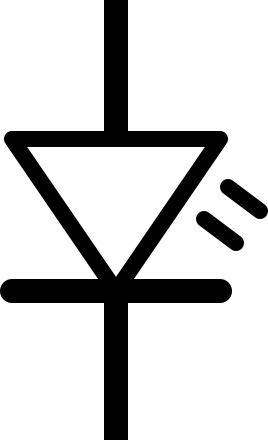
\includegraphics[scale=0.125]{LEDSymbol.png} & LED & An LED is represented by an arrow with a line across it, indicating that current can flow from positive to negative in the direction of the arrow, but it is blocked going the other way.  The LED symbol also has two short lines coming out of it, representing the fact that it emits light. \\
\end{tabular}
\end{center}


\chapter{Electronics Equations and Where They Come From}
\label{appendixElectronicsEquations}

% Thevenin Equivalent Equation
% Gain resistor equation

This appendix is a catalog of equations in electronics and where they came from for those who are curious.
This book is meant more for an introductory approach, but nonetheless many people are curious.
This chapter isn't for the faint of heart, and it may involve lots of math you haven't taken.
That's why it is stuck in an appendix.

However, if you are curious, these are the mathematical answers to your questions.

\section{Basic Formulas}

\subsection{Charge and Current Quantities}

\begin{itemize}
\item $1\textrm{ coulomb}  = 6.241509×10^18\textrm{ electrons}$ (how many electrons in a coulomb)
\item $I = \frac{dC}{dt}$ (current is the derivative of charge with respect to time)
\item $1A = 1\frac{C}{s}$ ($A$ = ampere; $C$ = coulomb; $s$ = second)
\item $3.6C = 1 mAh$ ($C$ = coulomb; $mAh$ is milliamp-hour,  a common unit for batteries)
\end{itemize}

\subsection{Volt Quantities}

Volts are basically measures of energy per unit of charge. Volts are also known as electromotive force (EMF), or $\epsilon$.  Volts can be expressed in a number of ways:

\begin{itemize}
\item $V = \frac{J}{C}$ ($J$ = joules; $C$ = coulombs)
\item $V = \frac{\textrm{potential energy}}{\textrm{charge}}$
\item $V = \frac{N\cdot m}{C}$ ($N$ = newtons; $m$ = meters; $C$ = coulombs)
\item $V = \frac{kg\cdot m^2}{A\cdot s^3}$ ($kg$ = kilograms; $m$ = meters; $A$ = amperes; $s$ = seconds)
\item $V = \frac{d\phi}{dt}$ (Faraday's law of induction---voltage is the derivative of the flux of the magnetic field with respect to time)
\end{itemize}

\subsection{Resistance and Conductance Quantities}

Resistance is in ohm's.  The inverse of resistance is conductance (the ability of current to flow through a wire) and is measured in Siemens (S).  The Seimens unit is also called a mho (ohm spelled backwards), and is sometimes marked by an upside down omega (℧).

\begin{itemize}
\item $G = \frac{1}{R}$ ($G$ = conductance in siemens, $R$ = resistance)
\item $G = \frac{I}{V}$ ($G$ = conductance; $I$ is current; $V$ is voltage)
\item $R = \frac{V}{I}$ (Ohm's law)
\end{itemize}

Individual materials have a resistivity ($\rho$).

\begin{equation}
R = \rho \cdot \frac{\textrm{length}}{\textrm{cross-sectional area}}
\end{equation}

In other words, from beginning to end, resistance decreases with cross-sectional area, and increases with length.

\subsection{Ohm's Law}

$V$ is voltage (in volts), $I$ is current (in amperes), and $R$ is resistance (in ohms).

\begin{equation}
V = I\cdot R
\end{equation}

\subsection{Power}

$P$ is in Watts.  The following hold true for DC circuits.  For AC circuits, they hold true if the resistance is actually an impedance.

\begin{itemize}
\item $P = V\cdot A$
\item $P = I^2R$
\item $P = \frac{V^2}{R}$
\end{itemize}

\subsection{Capacitance}

Capacitance is the ability to store charge.

The fundamental equation for a capacitor:

\begin{equation}
Q = V\cdot C
\end{equation}

$Q$ is the amount of charge stored, $V$ is the voltage across the terminals, and $C$ is the capacitance in farads.

The derivative of this equation with respect to time is:

\begin{equation}
\frac{dQ}{dt} = \frac{dV}{dt}\cdot C
\end{equation}

Because current is the derivative of charge, we can then say:

\begin{equation}
I = C\frac{dV}{dT}
\end{equation}

The capacitance of capacitors is given by the equation:

\begin{equation}
C = \epsilon_r\epsilon_0\frac{A}{d}
\end{equation}

Here $C$ is capacitance, $\epsilon_r$ is the dielectric constant of whatever separates the capacitor's plates, $\epsilon_0$ is the dielectric constant of free space, $A$ is the area of the plates in square meters, and $d$ is the distance between the plates in meters.

\subsection{Inductance}

The fundamental equation for an inductor is:

\begin{equation}
\phi = L\cdot I
\end{equation}

Here, $\phi$ is the flux of the magnetic field in Webers, $L$ is inductance in henries, and $I$ is current in amperes.
The derivative gives you voltage:

\begin{align}
\frac{d\phi}{dt} = L\frac{dI}{dt} \\
V = L\frac{dI}{dt}
\end{align}

In other words, the voltage produced is proportional to the change in current.

The inductance of a coil of wire can be calculated by:

\begin{equation}
L = \frac{\mu \cdot N^2 \cdot A}{l}
\end{equation}

Where $N$ is the number of turns of wire, $A$ is the area of the coil, $l$ is the length of the coil, and $\mu$ depends on the core being used.

\section{Semiconductors}

Components made from silicon are known as semiconductors, and have very useful non-linear properties.

\subsection{Diodes}

Diodes do not have a fixed voltage drop like we assume in this book.  
It is an exponential function, but is steep enough to act like a fixed $0.6\myvolt$ voltage drop for most purposes.
The actual equation is:

\begin{equation}
I = I_S (e^{\frac{V}{\eta V_T}} - 1)
\end{equation}

$I_S$ is the saturation current (depends on the construction of the diode), $V$ is the voltage, $\eta$ is either 1 for germanium or 2 for silicon, and $V_T$ is known as the thermal voltage (the amount of voltage created just by particles moving around at a given temperature, usually about $0.026\myvolt$ at room temperature).

\subsection{NPN BJT Transistors}

While we discussed general rules about BJT transistors, the technical model used to model them is known as the Ebers-Moll model.
This model is much more complex to use, which is why we don't discuss it much in the chapter.

There are also several different Ebers-Moll models, depending on the level of detail required.
The basic Ebers-Moll model for a conducting but unsaturated transistor is as follows:

\begin{equation}
I_E = I_S(e^{\frac{V_BE}{V_T}} - 1)
\end{equation}

In this $I_E$ is the emitter current (you can also use it for the collector current, since they are approximately equal).
$I_S$ is the saturation current of the base-emitter diode, and $V_T$ is the thermal voltage, just like for diodes.

% http://people.seas.harvard.edu/~jones/es154/lectures/lecture_3/bjt_models/ebers_moll/ebers_moll.html
% http://inderjitsingh87.weebly.com/uploads/2/1/1/4/21144104/the__ebers-moll_bjt_model.pdf
% http://ecetutorials.com/analog-electronics/ebers-moll-model-of-transistor/

\section{DC Motor Calculations}
\label{appDCMotorCalculations}

The voltage drop across a motor ($V_m$) is defined by the following equation:
\begin{align*}
V_m = V_b + R_m I_m
\end{align*}
where $V_b$ is the back EMF of the motor, $R_m$ is the internal resistance of the motor's wiring, and $I_m$ is the current flowing through the motor.
So, basically, just Ohm's law plus the back EMF generated by the spinning of the motor.

So how much back EMF is created?  We can determine that like this:
\begin{align*}
V_b = K_e \omega
\end{align*}
In this equation, $K_e$ varies by the motor, and is usually given in volts per RPM or volts per radians per second.
$\omega$ is merely the rotational speed in the units given.

Likewise, the torque generated can be determined from this equation:
\begin{align*}
T = K_T I_m
\end{align*}
In this equation, $K_T$ is the torque constant for the motor (be careful of the units), and $I_m$ is the current going through the motor.
Knowing the peak (stall) current, you can find the maximum torque available for the motor.

Interestingly, you can see that increasing the torque will actually affect, to some degree, the RPM of the motor.
The full equation for the voltage across the motor is:
\begin{align*}
V_m = K_e \omega + R_m I_m
\end{align*}

The torque will affect $I_m$.
That, in effect, will increase the voltage drop given by $R_m I_m$.
Given a fixed voltage source, this will leave less voltage available for the $K_e \omega$ part of the equation.
Since $K_e$ is a constant, that means that $\omega$ will be reduced to some extent.


\section{555 Timer Oscillator Frequency Equation}
\label{apOscillatorFreq}

In Chapter~\ref{chapOscillators} we learned to make oscillators using the 555 timer chip.
In the actual chapter, I wanted you to focus on actually learning what was happening with the 555 timer rather than using a formula.
However, there is a nice, simple formula that allows you to relate the resistor/capacitor network of the 555 timer to the final output frequency.

The formula is as follows:

\begin{equation}
f = \frac{1.44}{C(R_1 + 2 R_2)}
\end{equation}

In this equation, $f$ is the frequency, $R_1$ is the resistor coming from the supply voltage, $R_2$ is the resistor next to the capacitor, and $C$ is the timer capacitor.

To understand where this equation comes from, remember that frequency is just $\frac{1}{\textrm{period}}$.
We can use time constant formulas to find the period, and then just flip it to find the frequency.

If you recall, the period is just the total time it takes to complete a charge/discharge cycle.  
The 555 charges through \emph{both} $R_1$ and $R_2$, but only discharges through $R_2$.
Additionally, since it is just bouncing back-and-forth between $\frac{1}{3}$ and $\frac{2}{3}$ full, it only uses $0.693$ time constants.

Therefore, we can have two formulas, one for the time charging and one for the time discharging:

\begin{align*}
T_{\text{CHARGE}} &= 0.693 C (R_1 + R_2) \\
T_{\text{DISCHARGE}} &= 0.693 C R_2
\end{align*}

The total period is just these two time periods added together.
Therefore, you get:

\begin{align*}
T_{\text{PERIOD}} &= 0.693 C (R_1 + R_2) + 0.693 C R_2 \\
 &= 0.693 C((R_1 + R_2) + R_2) && \textrm{Factoring out $0.693 C$} \\
 &= 0.693 C(R_1 + 2 R_2) && \textrm{Regrouping}
\end{align*}

Since $f = \frac{1}{T_{\text{PERIOD}}}$, we can flip the above equation and get:

\begin{align*}
f &= \frac{1}{0.693 C(R_1 + 2 R_2)} \\
  &= \frac{1}{0.693}\frac{1}{C(R_1 + 2 R_2)} && \textrm{Regrouping} \\
  &\approx 1.44 \frac{1}{C(R_1 + 2 R_2)} \\
  &= \frac{1.44}{C(R_1 + 2 R_2)}
\end{align*}

At the end of the day, this is exactly what you did when you solved those problems, you just did it by hand instead of using a nice little formula.
All a formula does is encapsulate the things that you normally do anyway, but simplifies it down to a set of pre-defined steps.

I have a love/hate relationship with formulas.  
Formulas are nice because they are easy to use.
However, when you use them, it makes it easy to forget the basic facts behind them.
The basic facts are more important than the formula, because you can rearrange the basic facts and develop all sorts of formulas depending on your needs.
In fact, if you know the basic facts, and you know how to make formulas, if you ever forget a formula it is easy to determine one from the basic facts.
Therefore, while memorizing formulas is important, knowing \emph{why} formulas work is just as important, as it allows you to think more deeply and broadly and adapt your knowledge to new situations.

% Need to think more on this
\iffalse
\subsection{Current Gain Stabilization in BJT Common Emitter Applications}
\label{eqGainStabilizingEmitterResistorDCCommonEmitter}

% FIXME - should probably show two circuits

This section will show how we got the equation for the gain stabilizing emitter resistor you encountered in Chapter~\ref{chapTransistorIntro}.
We will need to imagine two circuits.
One before we add the emitter resistor (we will call this the \emph{nominal} circuit) and one after (we will call this the \emph{actual} circuit).
Since the goal is to do our calculations for base current on the circuit \emph{without} the emitter resistor, we will call this current the \emph{nominal base current}, and give it the symbol $I_N$.
All other values and currents will be determined from the \emph{actual} circuit.
The final gain between the nominal base current we calculated and the final collector current we will designate as $K$.
The values that are shared between the nominal and the actual circuit are $V_S$ (source voltage) and $V_B$ (base resistance).

\begin{align*}
K &= \frac{I_C}{I_N} && \textrm{this is our final gain} \\
I_N &= \frac{V_S - 0.6}{R_B} && \textrm{Ohm's Law for nominal base} \\
I_B &= \frac{V_S - V_B}{R_B} && \textrm{Ohm's Law for actual base} \\
V_B &= V_E + 0.6 && \textrm{transistor rules} \\
I_B &= \frac{V_S - (V_E + 0.6)}{R_B} && \textrm{substituting} \\
I_B &= \frac{V_S - V_E - 0.6)}{R_B} && \textrm{simplifying} \\
V_E &= R_E I_E && \textrm{Ohm's Law} \\
V_E &= R_E(I_B + I_C) && \textrm{substituting} \\
V_E &=  R_E I_B + R_E I_C && \textrm{distributing} \\
I_B &= \frac{V_S - (R_E I_B + R_E I_C) - 0.6}{R_B} && \textrm{substituting} \\
I_B &= \frac{V_S - R_E I_B - R_E I_C - 0.6}{R_B} && \textrm{simplifying} \\
I_C &= \beta I_B && \textrm{transistor beta equation} \\
I_C &= \beta \frac{V_S - R_E I_B - R_E I_C - 0.6}{R_B} && \textrm{substituting} \\
I_C &= \frac{\beta V_S - \beta R_E I_B - \beta R_E I_C - \beta 0.6}{R_B} \\
I_N &= \frac{V_S - 0.6}{R_B} && \textrm{Copied from Earlier} \\
K &= \frac{I_C}{I_N} && \textrm{This is the value we are looking for} \\
\frac{I_C}{I_N} &= \frac{\frac{\beta V_S - \beta R_E I_B - \beta R_E I_C - \beta 0.6}{R_B}}{\frac{V_S - 0.6}{R_B}} && \textrm{substituting} \\
\frac{I_C}{I_N} &= \frac{\beta V_S - \beta R_E I_B - \beta R_E I_C - \beta 0.6}{R_B} \frac{R_B}{V_S - 0.6} && \textrm{simplifying} \\
\frac{I_C}{I_N} &= \frac{\beta V_S - \beta R_E I_B - \beta R_E I_C - \beta 0.6}{V_S - 0.6} && \textrm{simplifying} \\
I_B &= \frac{I_C}{\beta} && \textrm{transistor beta definition} \\
\frac{I_C}{I_N} &= \frac{\beta V_S - \beta R_E \frac{I_C}{\beta} - \beta R_E I_C - \beta 0.6}{V_S - 0.6} && \textrm{substituting} \\
\frac{I_C}{I_N} &= \frac{\beta V_S - R_E I_C - \beta R_E I_C - \beta 0.6}{V_S - 0.6} && \textrm{simplifying} \\
\end{align*}
\begin{align*}
I_C(V_S - 0.6) = I_N(\beta V_S - R_E I_C - \beta R_E I_C - \beta 0.6) && \textrm{cross-multiplying} \\
I_C V_S - 0.6 I_C = I_N \beta V_S - I_N R_E I_C - I_N \beta R_E IC - I_N \beta 0.6 && \textrm{distributing} \\
I_C V_S - 0.6 I_C + I_N R_E I_C + I_N \beta R_E I_C =  I_N \beta V_S  -  I_N \beta 0.6 && \textrm{collecting $I_C$ terms} \\
I_C V_S - 0.6 I_C + \frac{V_S - 0.6}{R_B} R_E I_C + \frac{V_S - 0.6}{R_B} \beta R_E I_C =  I_N \beta V_S  -  I_N \beta 0.6 && \textrm{substituting some $I_N$ terms} \\
I_C V_S - 0.6 I_C R_B + V_S R_E IC - 0.6 R_E I_C + V_S \beta R_E I_C - 0.6 \beta R_E I_C =  R_B I_N \beta V_S  -  R_B I_N \beta 0.6 && \textrm{getting rid of fraction} \\
I_C(V_S - 0.6 R_B + V_S R_E - 0.6 R_E + V_S \beta R_E - 0.6 \beta R_E) =  I_N(R_B \beta V_S  -  R_B \beta 0.6) && \textrm{factoring} \\
\frac{I_C}{I_N} = \frac{R_B \beta V_S  -  R_B \beta 0.6}{V_S - 0.6 R_B + V_S R_E - 0.6 R_E + V_S \beta R_E - 0.6 \beta R_E}
\end{align*}

Now, this looks like a huge mess, and it is.
However, lets look at what happens with reasonable values.
Let's say our base resistor was $1\mykohm$ and the emitter resistor was $300\mykohm$.  
Let's also say that the source voltage if $5\myvolt$ and the transistor $\beta$ is 100.
What does this look like?

\begin{align*}
\frac{IC}{IN} &= \frac{R_B \beta V_S  -  R_B \beta 0.6}{V_S - 0.6 R_B + V_S R_E - 0.6 R_E + V_S \beta R_E - 0.6 \beta R_E} \\
\frac{I_C}{I_N} &= \frac{1000 \cdot 100 \cdot 5  -  1000\cdot 100 \cdot 0.6}{5 - 0.6 \cdot 1000 + 5 \cdot 300 - 0.6 \cdot 300 + 5\cdot 100 \cdot 300 - 0.6 \cdot 100 \cdot 300}
\end{align*}

This then becomes

\begin{align*}
\frac{I_C}{I_N} = \frac{500000 - 60000}{5 - 600 + 150000 - 180 + 1500 - 18000}
\end{align*}

Now, on the numerator, the dominating term is $500,000$, and on the bottom it is $150,000$.  
The other terms pale in comparison.
This will be true for most ``typical'' situations.
So, what makes up these two terms?

On the top, the $500,000$ term comes from $R_B \beta V_S$.
On the bottom, the $150,000$ term comes from $V_S \beta R_E$.
Therefore, a simplified look at this equation is just:

\begin{align*}
\frac{I_C}{I_N} = \frac{R_B \beta V_S}{V_S \beta R_E} && \textrm{these are the dominant factors} \\
\frac{I_C}{I_N} = \frac{R_B}{R_E} && \textrm{cancelling out factors} \\
\end{align*}

So, even though it isn't an exact result, you can see that the ratio between the actual current in the real circuit and the nominal base current that we calculated will be given by $\frac{R_B}{R_E}$.
\fi

\section{Voltage Gain Stabilization in BJT Common Emitter Applications}
\label{apTransistorVoltageGain}

The previous section told you how to stabilize the current gain from an emitter resistor, with the final gain being $\frac{R_B}{R_E}$.
For \emph{voltage} gain, the final gain is limited by $\frac{R_C}{R_E}$, and we will show that here using similar reasoning.

The voltage at the emitter and the base will be:

\begin{align*}
V_E &= I_E R_E \\
V_B &= V_E + 0.6 \\
V_B &= I_E R_E + 0.6 \\
\end{align*}

The voltage at the collector will be:

\begin{align*}
V_C &= I_C R_C
\end{align*}

However, the collector current and the emitter current are very close.
Therefore, we can simplify this to say:

\begin{align*}
V_C &= I_E R_C
\end{align*}

We can then divide our equation for the collector voltage by our equation for the base voltage, and get:

\begin{align*}
\frac{V_C}{V_B} &= \frac{I_E R_C}{I_E R_E + 0.6}
\end{align*}

If we remove the diode voltage (which has relatively little influence overall), this simply becomes:

\begin{align*}
\frac{V_C}{V_B} &= \frac{I_E R_C}{I_E R_E} \\
 &= \frac{R_C}{R_E}
\end{align*}

Therefore, the ratio of base voltage to output voltage is approximately equal to the ratio of collector to emitter.
However, also keep in mind that this is the voltage \emph{drop} in the collector.  
What we actually send to the output is actually our supply voltage with $V_C$ subtracted from it.

As you can see, there is a lot of simplification involved.
However, such simplifications allow us to think more clearly about our circuits.
Since there are so many moving parts, looking for and finding the dominating factors is very important.

Note that this is important in life, too.
Sometimes we get so enmeshed in the details that we forget what factors dominate our quality of life.
Finding out what the important factors are help us to focus on the things that matter most, and let the details sort themselves out.

\section{The \thev Formula}

In Chapter~\ref{chapPartialCircuits}, we used two formulas which allowed us to calculate the \thev Equivalent circuit for circuits experimentally.
Equations~\ref{eqThevEqVoltExp} and~\ref{eqThevEqResExp} seem strange and complicated, but they are actually directly deducible from Ohm's law and the concept of an equivalent circuit.

The \thev Theorem states that any combinations of voltage sources and resistances can be replaced by a single voltage source and a single resistance.  
We will call this our \thev voltage source ($V_T$) and our \thev impedance ($R_T$).
If we hook up a load (i.e., a fixed resistance) across the output terminals of this circuit, we will know the resistance that was added (because \emph{we} added it), and we can measure the voltage drop across the resistor easily enough with a multimeter or oscilloscope.

We will need to measure this using two different loads because we have two unknowns---$V_T$ and $R_T$.
Using two different loads will give us two different equations using Ohm's law that will allow us to solve for two variables.
We will call our lower-resistance load $R_L$ and the voltage drop across the $R_L$ resistor will be $V_L$.
Likewise, our higher-resistance load we will call $R_H$ and the voltage drop across it will be $V_H$.
The current running through each of these loads ($I_L$ and $I_H$) can be given by:

\begin{align*}
V_L &= I_L \cdot R_L \\
V_H &= I_H \cdot R_H
\end{align*}

That is just simply Ohm's law.
We can also use Ohm's law to develop equations for the whole circuit, including the \thev Equivalent voltage and impedance.
Remember, because of the current rules, whatever current is flowing through our resistor must also be flowing in our \thev Equivalent impedance.
Therefore, the \thev Equivalent voltage will be the current multiplied by the two impedances together.
Therefore, this yields the following equations:

\begin{align*}
V_T &= I_L (R_L + R_T) \\
V_T &= I_H (R_H + R_T)
\end{align*}

Both of these equations solve for $V_T$, given an unknown of $R_T$.  
We can also rearrange either of these to solve for $R_T$.  
Let's rearrange the first one to do that:

\begin{align*}
V_T &= I_L (R_L + R_T) && \textrm{Original equation} \\
\frac{V_T}{I_L} &= R_L + R_T  && \textrm{Divide both sides} \\
\frac{V_T}{I_L} - R_L &= R_T && \textrm{Subtract $R_L$} \\
R_T &= \frac{V_T}{I_L} - R_L && \textrm{Solved for $R_T$} \\
\end{align*}

This is the same as Equation~\ref{eqThevEqResExp}.
However, it requires $V_T$ to work.
Now that we have an equation for $R_T$, we can substitute that back in and get an equation for $V_T$ without using $R_T$.
Using basic algebra manipulations, we can do the following:

\begin{align*}
V_T &= I_H (R_T + R_H) && \textrm{Original equation} \\
V_T &= I_H R_T + I_H R_H && \textrm{Distributive rule} \\
V_T &= I_H (\frac{V_T}{I_L} - R_L) + I_H R_H && \textrm{Substituting for $R_T$} \\
V_T &= I_H \frac{V_T}{I_L} - I_H R_L + I_H R_H && \textrm{Distributing} \\
V_T - I_H \frac{V_T}{I_L} &= - I_H R_L + I_H R_H && \textrm{Get the $V_T$s together} \\
V_T(1 - \frac{I_H}{I_L}) &= I_H (R_H - R_L) && \textrm{Factor both sides} \\
V_T &= \frac{I_H (R_H - R_L)}{1 - \frac{I_H}{I_L}} && \textrm{Divide both sides} \\
V_T &= \frac{\frac{V_H}{R_H} (R_H - R_L)}{1 - \frac{V_H R_L}{R_H V_L}} && \textrm{Replace currents with Ohm's law equivalents ($\frac{V}{R}$)}
\end{align*}

As you can see, this is Equation~\ref{eqThevEqVoltExp}.

% Basic algebra is easier but gives a different (slightly more complex) form
%I_H V_T &= I_H I_L R_L + I_H I_L R_T && \textrm{Multiply both sides by $I_H$} \\
%I_L V_T &= I_H I_L R_H + I_H I_L R_T && \textrm{Multiply both sides by $I_L$} \\
%I_H V_T - I_L V_T &= I_H I_L R_L + I_H I_L R_T - (I_H I_L R_H + I_H I_H R_T) && \textrm{Subtract both equations} \\
%I_H V_T - I_L V_T &= I_H I_L R_L + I_H I_L R_T - I_H I_L R_H - I_H I_H R_T && \textrm{Distribute the subtraction} \\
%I_H V_T - I_L V_T &= I_H I_L R_L - I_H I_L R_H  && \textrm{Simplify} \\
%V_T (I_H - I_L) &= I_H I_L R_L - I_H I_L R_H && \textrm{Regroup the left-hand side} \\
%V_T &= \frac{I_H I_L R_L - I_H I_L R_H}{I_H - I_L} && \textrm{Divide both sides by $I_H - I_L$} \\
%V_T &= \frac{I_H I_L (R_L - R_H)}{I_H - I_L} && \textrm{Regroup the top} \\
%V_T &= \frac{\frac{V_H}{R_H} \frac{V_L}{R_L} (R_L - R_H)}{\frac{V_H}{R_H} - \frac{V_L}{R_L} && \textrm{Replace currents with their Ohm's law equivalents}

\section{Electronics and Calculus}

Calculus is a favorite subject of mine, and many parts of electronics make a lot of sense in the light of Calculus.

\subsection{Current and Voltage}
First of all, recognize that electronics includes both static and dynamic quantities. 
Charge, for instance, is a static quantity.
Current, though, is the \emph{movement} of charge, and thus is a dynamic quantity.
Current entering or leaving a point can be written as a differential:
\begin{equation}
I = \frac{\dQ}{\dt}
\end{equation}
Like current, voltage is a dynamic quantity, which is the change in the magnetic flux ($\phi$):
\begin{equation}
V = \frac{\deriv{\phi}}{\dt}
\end{equation}

\subsection{Capacitors and Inductors}

The static equation governing a capacitor is
\begin{equation}
Q = V \cdot C
\end{equation}
where $Q$ is the charge, $V$ is the voltage, and $C$ is the capacitance.
Taking the derivative of both sides, this can be converted into a dynamic equation. 
\begin{equation}
\frac{\dQ}{\dt} = C\frac{\dV}{\dt}
\end{equation}
Since $\frac{\dQ}{\dt} = I$ we can rewrite this as
\begin{equation}
I = C\frac{\dV}{\dt}.
\end{equation}
What this means is that the current is proportional to the \emph{change} in voltage.

The static equation governing an inductor is similar:
\begin{equation}
\phi = L \cdot I
\end{equation}
Taking the derivative of both sides yields
\begin{equation}
\frac{\deriv{\phi}}{\dt} = L \cdot \frac{\deriv{I}}{\dt}
\end{equation}
Since $V = \frac{\deriv{\phi}}{\dt}$, this can be rewritten as
\begin{equation}
V = L \cdot \frac{\deriv{I}}{\dt}.
\end{equation}
In other words, on inductors, the voltage is proportional to the change in current.

\subsection{Time Constants}

If an ideal capacitor were connected to an ideal voltage source, then the capacitor would charge instantaneously.


\chapter{Integrated Circuit Naming Conventions}
\label{appICNaming}

% Source information
% 4000 vs 74xx - http://www.elecdude.com/2014/07/differences-in-cmos-4000-series-74ls-74hc-74hct.html
% microwatts
% Simple logic gates - http://www.eng.utah.edu/~cs6710/handouts/AppendixB/appendixB.doc2.html
% http://www.avrfreaks.net/forum/does-hct-vs-hc-still-matter-5v
% http://www.righto.com/2014/09/reverse-engineering-counterfeit-7805.html
% Simple digital computer - http://www.simpledigitalcomputer.com/
% Open collector info - http://denethor.wlu.ca/pc200/lectures/lgcocbeam.pdf
% Logic Level - https://en.wikipedia.org/wiki/Logic_level / http://www.allaboutcircuits.com/textbook/digital/chpt-3/logic-signal-voltage-levels/
% TTL - https://en.wikipedia.org/wiki/Transistor%E2%80%93transistor_logic
% TTL/CMOS comparison - http://design-technology-in-stem.x10.mx/07%20Digital%20Electronics/02%20TTL%20and%20CMOS%20ICs/digital%20IC%20introduction/digtal%20IC's%20background%20introduction.html
% TTL/CMOS level shifting - http://www.instructables.com/id/Level-Shifting-Between-TTL-and-CMOS/?ALLSTEPS
% 7400 series history - https://en.wikipedia.org/wiki/7400_series
% 7400 series partlist -  https://en.wikipedia.org/wiki/List_of_7400_series_integrated_circuits
% 4000 series history - https://en.wikipedia.org/wiki/4000_series
% 4000 series partlist - https://en.wikipedia.org/wiki/List_of_4000_series_integrated_circuits
% Manufacturer prefixes - http://www.interfacebus.com/logic_prefix.html / https://en.wikibooks.org/wiki/Practical_Electronics/Manufacturers_Prefix / http://www.logwell.com/tech/components/ic_id.html / https://dmohankumar.wordpress.com/2012/04/24/know-the-meaning-of-transistor-and-ic-codes/
% General logic numbering - http://www.radio-electronics.com/info/data/semicond/logic-ic-families-technologies/ic-numbering.php 
% 74 families - http://www.chip1stop.com/web/AUS/en/tutorialContents.do?page=051 / http://www.chip1stop.com/web/AUS/en/tutorialContents.do?page=050
% Suffix table - http://www.chip1stop.com/web/AUS/en/tutorialContents.do?page=052
% CMOS/TTL discussion - https://www.physicsforums.com/threads/high-low-impedances-by-ttl-logic.57886/
% CMOS/TTL long - http://www.lns.cornell.edu/~ib38/teaching/p360/lectures/wk09/l26/EE2301Exp3F10.pdf
% Making chip numbers more visible - http://electronics.stackexchange.com/questions/5186/how-to-read-the-text-printed-on-top-of-every-ic
% General identification guide - http://how-to.wikia.com/wiki/How_to_identify_computer_chips_or_integrated_circuits_on_circuit_boards
%
% Note that on ebay it is best just to look at the part and make sure the picture is DIP!
% 

The naming conventions for ICs can be bewildering at first.
In truth, there is no official standard for chip names, but there are some conventions that are often followed.
When a chip is invented, the company that invented it assigns it a part number.
However, the courts have ruled that part numbers cannot be copyrighted.
Therefore, if another manufacturer makes a similar or identical chip with the same pinout, they will often use the same part number.

\section{Logic Chip Basic Conventions}

Logic chips are often broken up into two families based on the voltage levels that they expect and produce.
\glossterm{TTL} (which stands for transistor-to-transistor logic) and an old standard for logic chips which usually operate at $5\myvolt$.
TTL chips consider a signal to be ``false'' when it is below $0.8\myvolt$ and ``true'' when it is above $2.2\myvolt$, and can break if they receive voltages significantly higher than $5\myvolt$.
Between $0.8\myvolt$ and $2.2\myvolt$ is a region where the resulting value is unpredictable.
TTL originally referred to \emph{how} the logic chips were constructed, but now it usually refers to the expected input/output levels of the chip.

\glossterm{CMOS} is a newer technology, and with it came a newer standard for how logic levels are interpreted.  
CMOS chips support a much wider supply voltage range than TTL, but their logic levels are a little different.
For CMOS, false is from $0\myvolt$ to one-third of the supply voltage (whatever it is---CMOS can usually operate from $3\myvolt$ to $15\myvolt$), and true is from two-thirds of the supply voltage to the full supply voltage.

Chips are often made in a series---a whole set of chips which all perform complementary functions.
The most common series of logic chips is the 7400 series originally designed by Texas Instruments.
The 7400 series started as a set of TTL chips.
Some common chips in this series is the 7400 itself (a quad NAND gate), the 7408 (a quad AND gate), and the 7432 (a quad NOR gate).

Chips names will often have a prefix that relates to either their manufacturer or the company that originally designed them.
As some examples, National Semiconductor chips are usually prefixed with LM, Texas Instruments chips have a whole slew of prefixes, including SN and TI, Motorola chips usually have an MC prefix, and Signetics usually has an NE prefix.
There are many others, but this is just to give you an example.
The 7400 series usually has part numbers starting with SN74 because TI built them.
So, a SN7408 is an AND gate based on designs by TI.

Now, the series is 7400.  
The last two digits refers to the function and pinout of the chips.
That is, in the 7400 series, ``08'' will refer to quad AND gates which all have the same pin configuration.
However, sometimes they will insert letters in-between ``74'' and ``08.''
This usually refers to some modification to the electrical characteristics of the chip.
For instance, a low-power version of the 7400 series have a ``74LS'' prefix.
So, the ``SN74LS08'' chip is a version of the 7408 (i.e., has the same pinout and function) that was originally designed by TI (the SN prefix) but is built for lower power consumption (LS).

Then, part numbers often have suffixes as well.
Suffixes often refer to some external characteristic of the chip.
For instance, in Chapter~\ref{chapIC}, we mentioned different chip packages, such as DIP and SMD.
These different packages will have different suffixes.
For the 7400 series, the DIP package is usually suffixed with ``P,'' so an SN74LS08P is the DIP version of the SN74LS08, and the NS74LS08NSR is an SMD version.
You may also have suffixes which are based on temperature, hardiness, and even occasionally electrical output characteristics.

Sometimes, if a different manufacturer builds the same chip, they may change the manufacturer code and use different suffixes.  
For instance, Texas Instruments sells a SN74HC08P, which is a DIP 7408 which uses CMOS levels up to $6\myvolt$ (that's what the HC is for).
Essentially the same chip is available from Fairchild, which calls it the MM74HC08N.
The MM prefix is one that Fairchild uses, it is the same 74HC08 chip, and, for Fairchild, they use an ``N'' suffix to designate a DIP chip.

As I mentioned, these are only conventions, not standards, so they don't always apply.
However, they can be helpful, so that you know that if someone specifies a 7432 chip, and you see part numbers that say SN74LS32P, you might be able to determine that this at least has some relationship to the chip you are looking for.

% FIXME - table of common chip prefixes by family
%       - table of device numbers by family
%

\chapter{Simplified Datasheets for Common Devices}
\label{appSimplifiedDatasheets}

\fixme{need content}


\end{document}

%
% FET vs BJT sources - http://www.eetimes.com/document.asp?doc_id=1272218 https://www.physicsforums.com/threads/bjt-vs-mosfet-amplifiers.443870/ https://www.physicsforums.com/threads/when-to-use-a-bjt-or-fet.640242/ http://forum.allaboutcircuits.com/threads/when-bjt-are-used-as-amplifier-and-when-fet-are-used-as-amplifier.64434/ http://www.learningaboutelectronics.com/Articles/BJT-vs-FET.php  https://www.quora.com/What-are-the-pros-and-cons-of-BJT-versus-FET-transistor
%
%
% FIXME - be sure to include non-math exercises in each section for younger learners who are just trying to get a conceptual grasp
% FIXME - should have drawing questions a lot more - start with drawing how the breadboard is connected
% FIXME - rearrange early chapters to have more than one on resistance and series and parallel
% FIXME - should have an appendix with a bunch of math
